% \documentclass[draft]{article}
\documentclass{article}

\title{Income and Consumption Inequality in Taiwan, 1981 - 2023}
\author{Bo-Yan Huang\thanks{Department of Economics, National Taiwan University, Taipei, Taiwan. Email: \href{mailto:boyanhuangwork@gmail.com}{boyanhuangwork@gmail.com}.}}
\date{Last Updated: November 2026\\ Original Version: June 2025}

% Bring in setting.tex
\usepackage[a4paper,top=2cm,bottom=2cm,left=3cm,right=3cm,marginparwidth=1.75cm]{geometry}
\usepackage{graphicx}
\usepackage{notoccite}
\usepackage[colorlinks=true, allcolors=blue]{hyperref}
% \usepackage{chngcntr}
% \usepackage{titlesec}
\usepackage{footnotebackref}
\usepackage{setspace}
\usepackage{subcaption}
\usepackage{booktabs}
\usepackage{mwe}
% \usepackage{caption}
% \usepackage{fancyhdr}
\usepackage{amsmath}  
\usepackage[title, titletoc]{appendix}
\usepackage[style=apa]{biblatex}
\usepackage{titling}
\addbibresource{mybib.bib}

% Print misc titles (data sources) without the default quoting, in the
% bibliography and in citations.
\DeclareFieldFormat[misc]{title}{{#1}}
\DeclareFieldFormat[misc]{citetitle}{{#1}}

\setstretch{1.3}
\setlength\parindent{2em}
\numberwithin{figure}{section}

\newcommand{\citelink}[2]{\hyperlink{cite.\therefsection @#1}{#2}}

\begin{document}

\maketitle

\vspace{-1cm}
\begin{center}
    \href{https://github.com/Bo-Yan-Huang/consumption-inequality/blob/main/Income-and-Consumption-Inequality-in-Taiwan-LATEST.pdf}{[Please click here for the latest version.]} 
\end{center}

\begin{abstract}
    This paper analyzes income and consumption inequality in Taiwan from 1981 to 2023 using household-level data from the Survey of Family Income and Expenditure. 
    Earnings inequality rose mainly before 2002, and by less than in the United States over a comparable span, with the burden falling most heavily on low-income households during recessions.
    Government redistribution through taxation and welfare programs has played a stabilizing role, though its effectiveness varies across crises. 
    Consumption inequality has remained stable or declined, reflecting the role of savings, borrowing, and family support, as well as slower consumption growth among wealthier households. 
    Together, these patterns highlight a divergence between income and consumption dynamics and signal potential structural vulnerabilities in Taiwan's economic landscape.
\end{abstract}

\section{Introduction}
\label{sec:introduction}

In Taiwan, the evolution of economic inequality is often overshadowed by other topics in the field of economics.
However, understanding the dynamics of inequality is crucial for comprehending the broader economic landscape. 
Most studies on inequality in Taiwan have focused on the income distribution and income gaps, with less attention given to consumption inequality.
For instance, Chang, Lin, and Lee (\citeyear{TW_classes_inc}) analyze personal income in Taiwan from 1990 to 2020.
Applying an Age-Period-Cohort (APC) model, they find that income gaps by education and social class widened over this period, and that the gap between the baby boomers and millennials has not narrowed. 
Chang (\citeyear{TW_party_inc_ineq}) focuses on how political parties shape government redistribution and income inequality.
The author finds that the Democratic Progressive Party's (DPP) share of seats in the Legislative Yuan is negatively correlated with income inequality. However, a DPP president is negatively correlated with redistribution, which worsens income inequality in the long run.
Both studies use the Survey of Family Income and Expenditure (SFIE) as their primary dataset. This repeated cross-sectional survey, started in 1978 and conducted yearly, provides detailed information on Taiwan's household income and expenditure patterns.

Consumption inequality has been less frequently studied in Taiwan. Hong (\citeyear{TW_consumption_inequality}) uses the SFIE from 1980 to 2007 to analyze the evolution of consumption inequality in Taiwan, focusing on a decomposition of the Gini coefficient and on income and consumption growth by percentile.
The study finds that consumption inequality decreased after 1996 mainly because rising medical and rent expenditures had an equalizing effect, and it links the rise of medical expenditure to population aging.
However, the decrease in consumption inequality could be a double-edged sword, since another reason for the decline is the low consumption growth of wealthy families, which could lead to economic stagnation.

One reason for the lack of attention to consumption in Taiwan and other countries is the difficulty in measuring consumption accurately.
First, unlike income, which can be directly observed through tax records, consumption is often inferred from expenditure data that the government does not document.
Therefore, consumption data are mostly collected through surveys, which have smaller samples and are more prone to measurement error and bias.
Currently, the SFIE is the only survey that provides detailed information on household consumption in Taiwan, while the Consumer Expenditure Survey (CE) is the only one in the US (Attanasio \& Pistaferri, \citeyear{JEP_Consumption_Inequality}).

Second, the transformation from expenditure to consumption is not straightforward. Surveys like the SFIE typically report household expenditures, which may not accurately reflect households' actual consumption.
For example, households may purchase goods in bulk or invest in durable goods, which can lead to discrepancies between expenditure and consumption. Most surveys lack information on the stock of durable goods and their current value.
Another example is that consumption can be produced at home from time and goods, such as childcare and home-cooked meals. Also, households may have different preferences for leisure and consumption, which can lead to differences in how they allocate their resources.
The most challenging problem to overcome is the assumption that all households face the same prices for goods and services. This assumption violates the nature of durable goods such as housing and automobiles, whose prices vary enormously. Ignoring these differences can lead to an inaccurate representation of consumption patterns and inequality.

This paper uses SFIE data to comprehensively analyze income and consumption inequality in Taiwan from 1981 to 2023 to fill in the missing pieces of inequality dynamics after 2008. This is interesting because economic growth in Taiwan has slowed since the 2008 financial crisis, and the COVID-19 pandemic has further exacerbated the situation.
The income distribution between households was stable before 1994, and the Gini coefficient for individual earnings stabilized at around 0.30 due to many factors (Bourguignon, Fournier, \& Gurgand, \citeyear{TW_stable_dist}).
However, the Gini coefficient for household earnings has increased since 1994, reaching 0.35 in 2023, as shown in the top right panel of Figure \ref{fig:Indi_to_HH}.
This suggests that economic inequality will become a problem after economic growth slows down, even in a country such as Taiwan, whose income distribution was previously stable.
The paper is organized as follows: Section \ref{sec:data} describes the data used in the analysis, Section \ref{sec:household_inequality} presents the household-level inequality measures, including earnings, consumption, and their cyclical dynamics, and Section \ref{sec:conclusion} concludes.

\section{Data}
\label{sec:data}

% \subsection{Survey of Family Income and Expenditure (SFIE)}
\subsection{Survey of Family Income and Expenditure (SFIE)}

The data used in this paper are the \citelink{DGBAS_SFIE}{SFIE} from 1981 to 2023, a repeated cross-sectional survey conducted annually since 1978 by the Directorate-General of Budget, Accounting and Statistics (\citeauthor{DGBAS_SFIE}) in Taiwan.
The survey provides a rich dataset for analyzing income and expenditure patterns, including earnings, private transfers, asset income, government transfers, and consumption expenditures.
The survey samples around 16,000 households each year. However, the share of missing values in some items, such as the labor earnings and industry earnings shown in Figure \ref{fig:missing}, is increasing.
\begin{figure}
    \centering
    \begin{subfigure}[t]{0.475\textwidth}
        \centering
        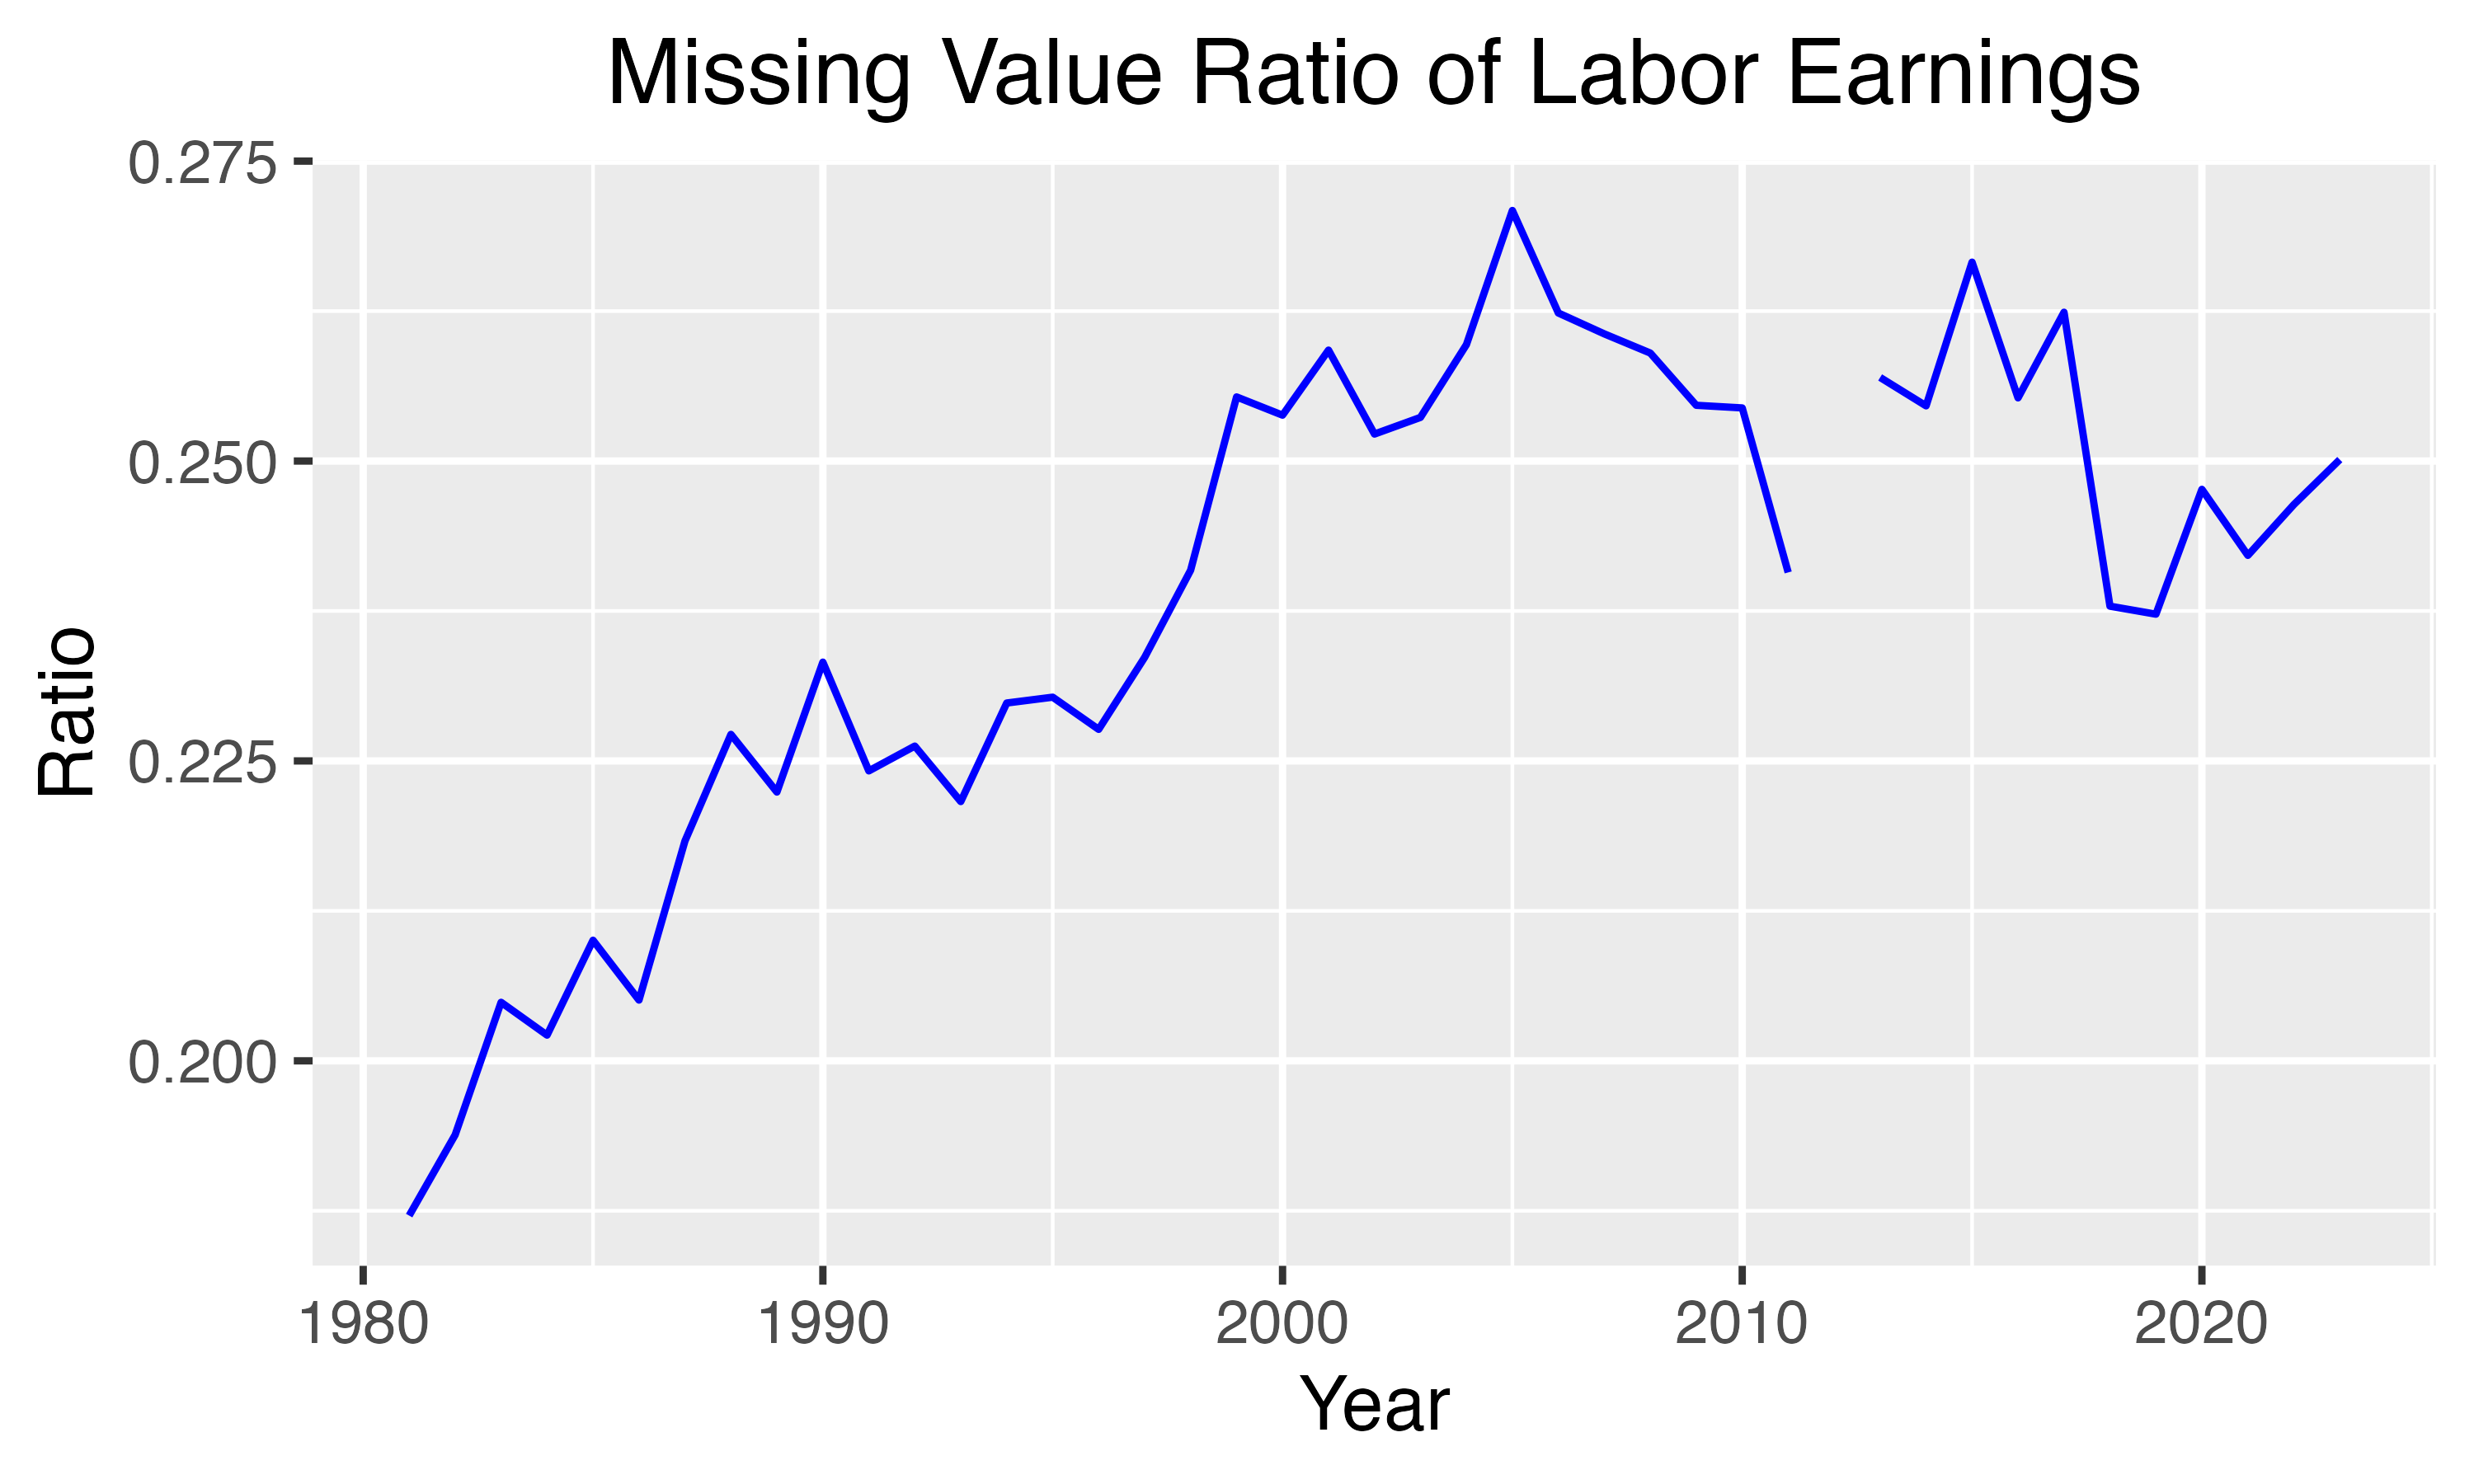
\includegraphics[width=\textwidth]{figures/missing/itm190.png}
    \end{subfigure}
    \begin{subfigure}[t]{0.475\textwidth}
        \centering
        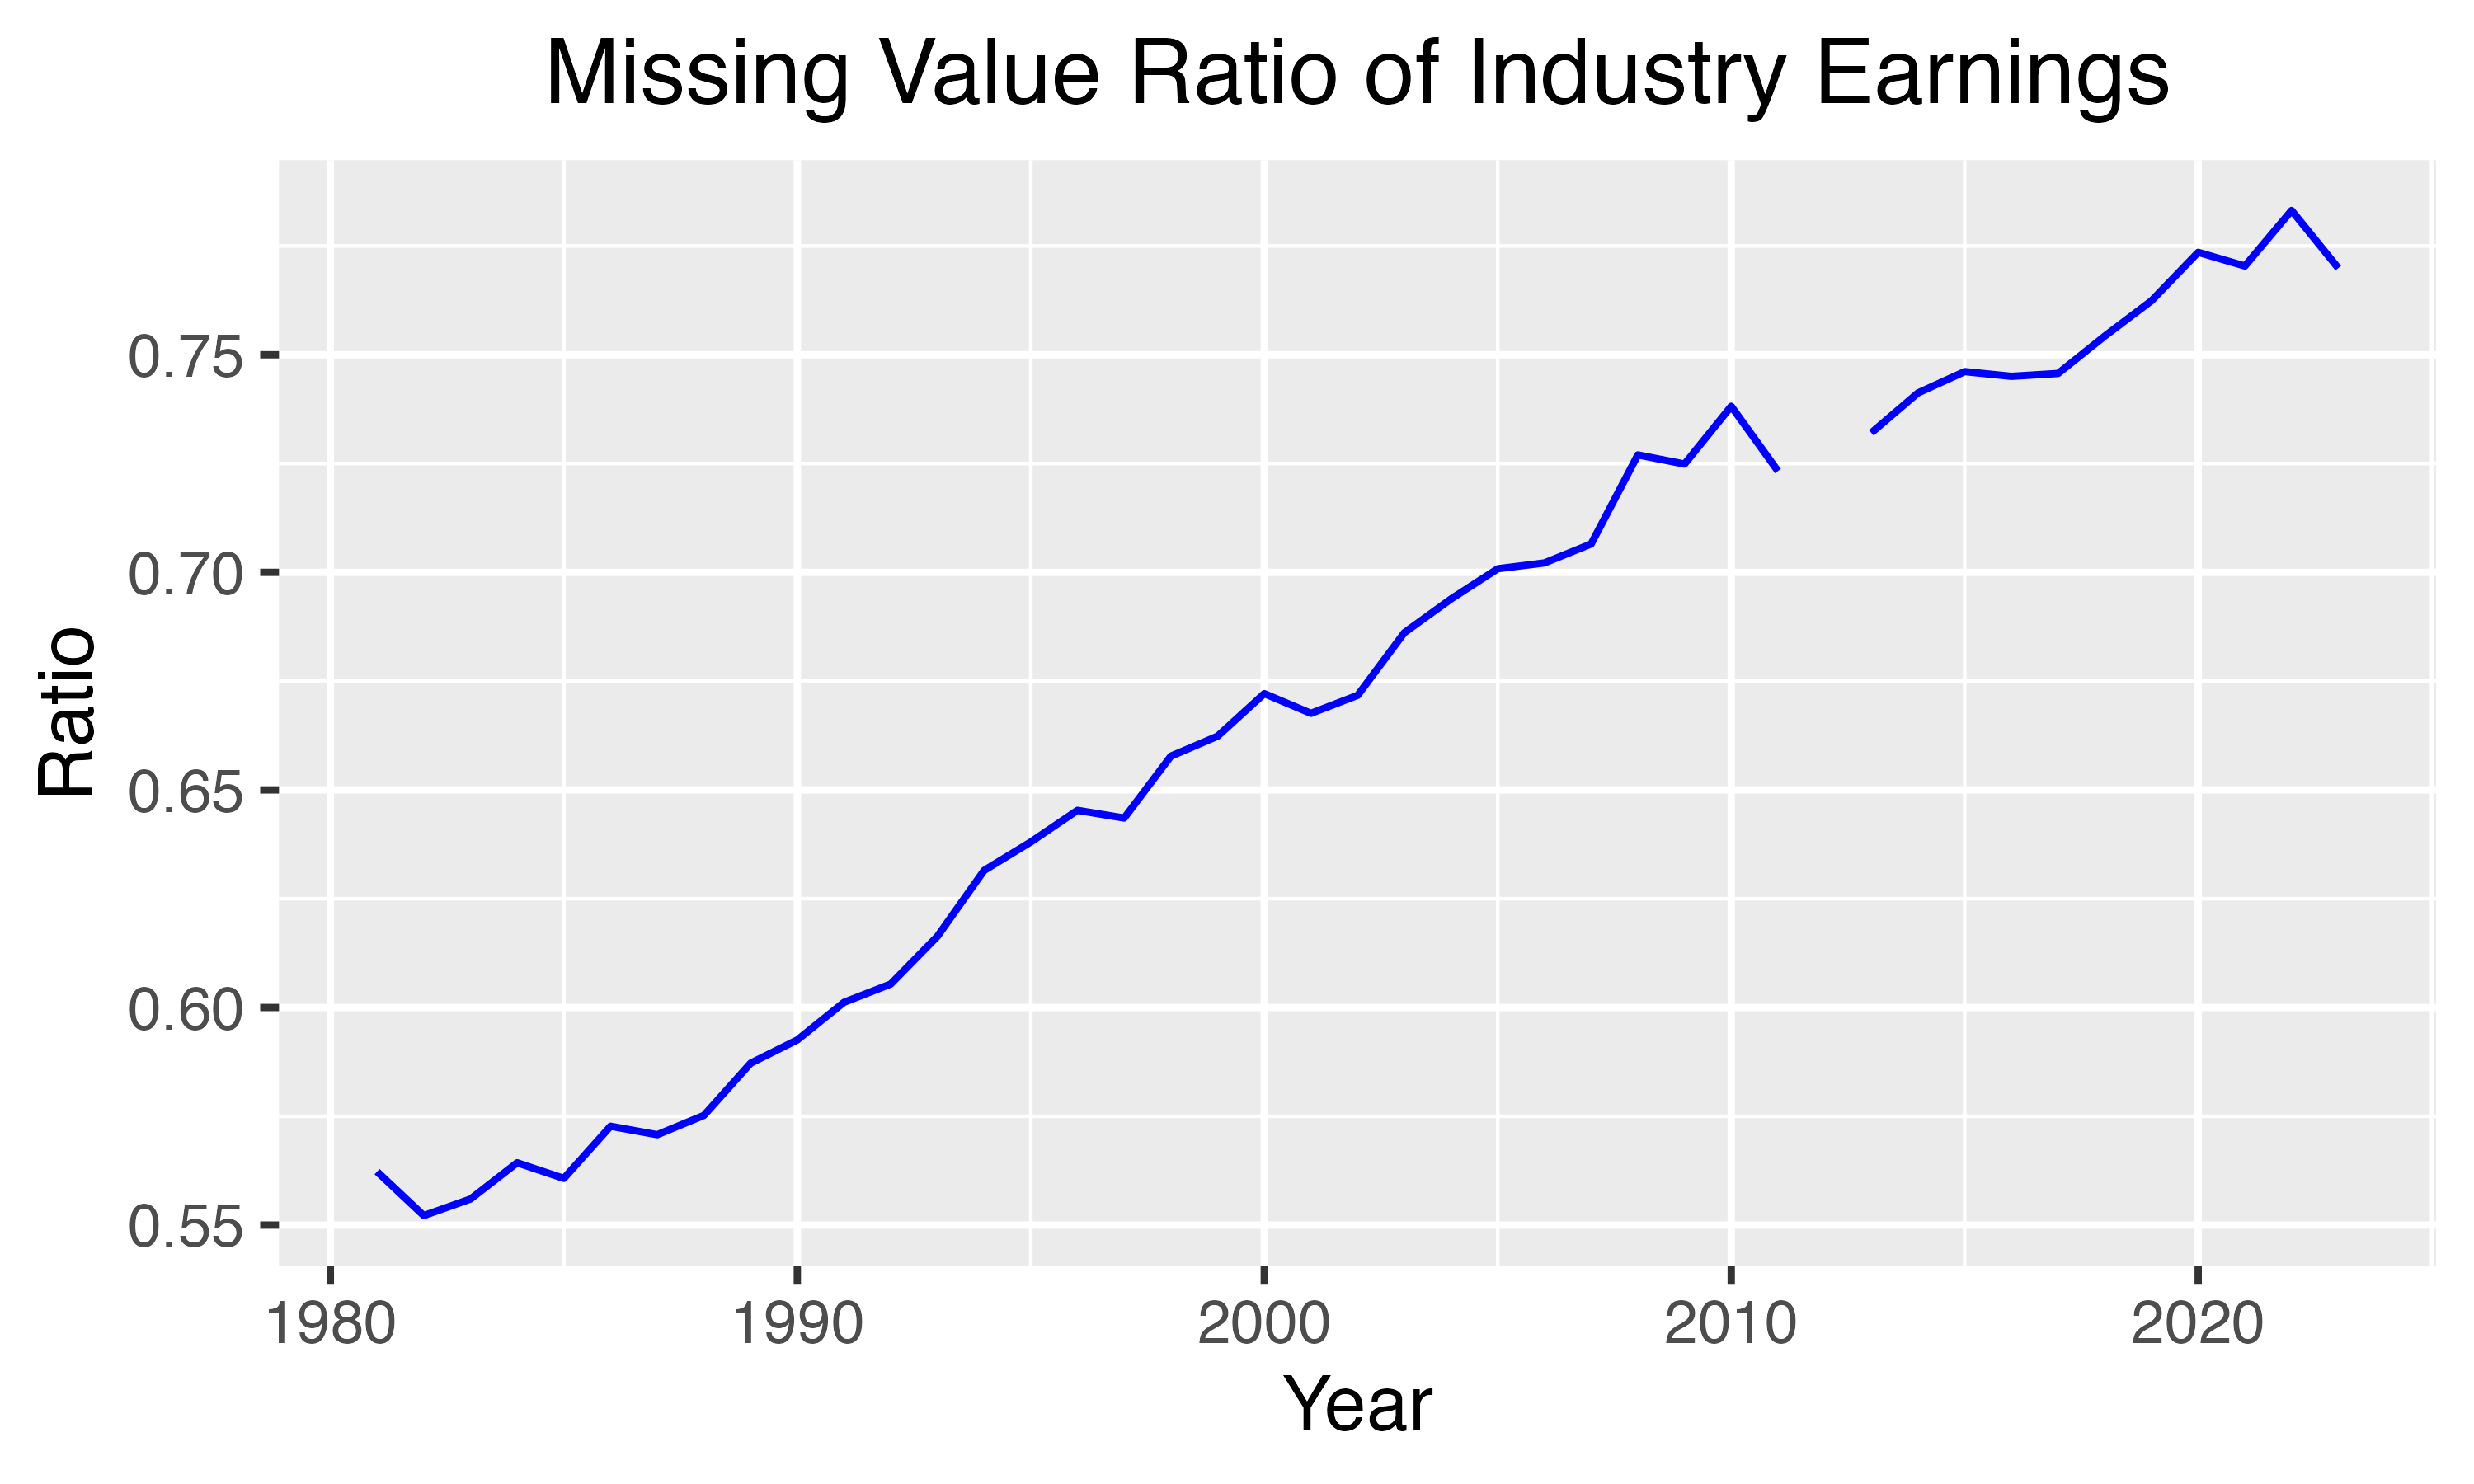
\includegraphics[width=\textwidth]{figures/missing/itm240.png}
    \end{subfigure}
    \caption{Missing Rate of Labor Earnings and Industry Earnings in SFIE}
    \label{fig:missing}
\end{figure}
In the SFIE, both a true zero and a non-response are recorded as missing values, so the two cannot be separated. 
Treating every missing value as zero would understate income and consumption levels at the bottom of the distribution.
The gap in 2012 in Figure \ref{fig:missing} has a different cause: the SFIE data file for 2012 contains all the demographic information, but every income and expenditure value is missing.
Section \ref{sec:sample} sets out how the analysis sample is built from these data.

\subsection{CPI Adjustment}

The SFIE provides nominal values for income and expenditures, which need to be adjusted for inflation to obtain real values. 
The price deflator used in this paper is the Consumer Price Index (\citelink{DGBAS_CPI}{CPI}) provided by the \citeauthor{DGBAS_CPI}.
Figure \ref{fig:CPI} shows the CPI in Taiwan from 1981 to 2023, normalized to 100 in 2021.
\begin{figure}
    \centering
    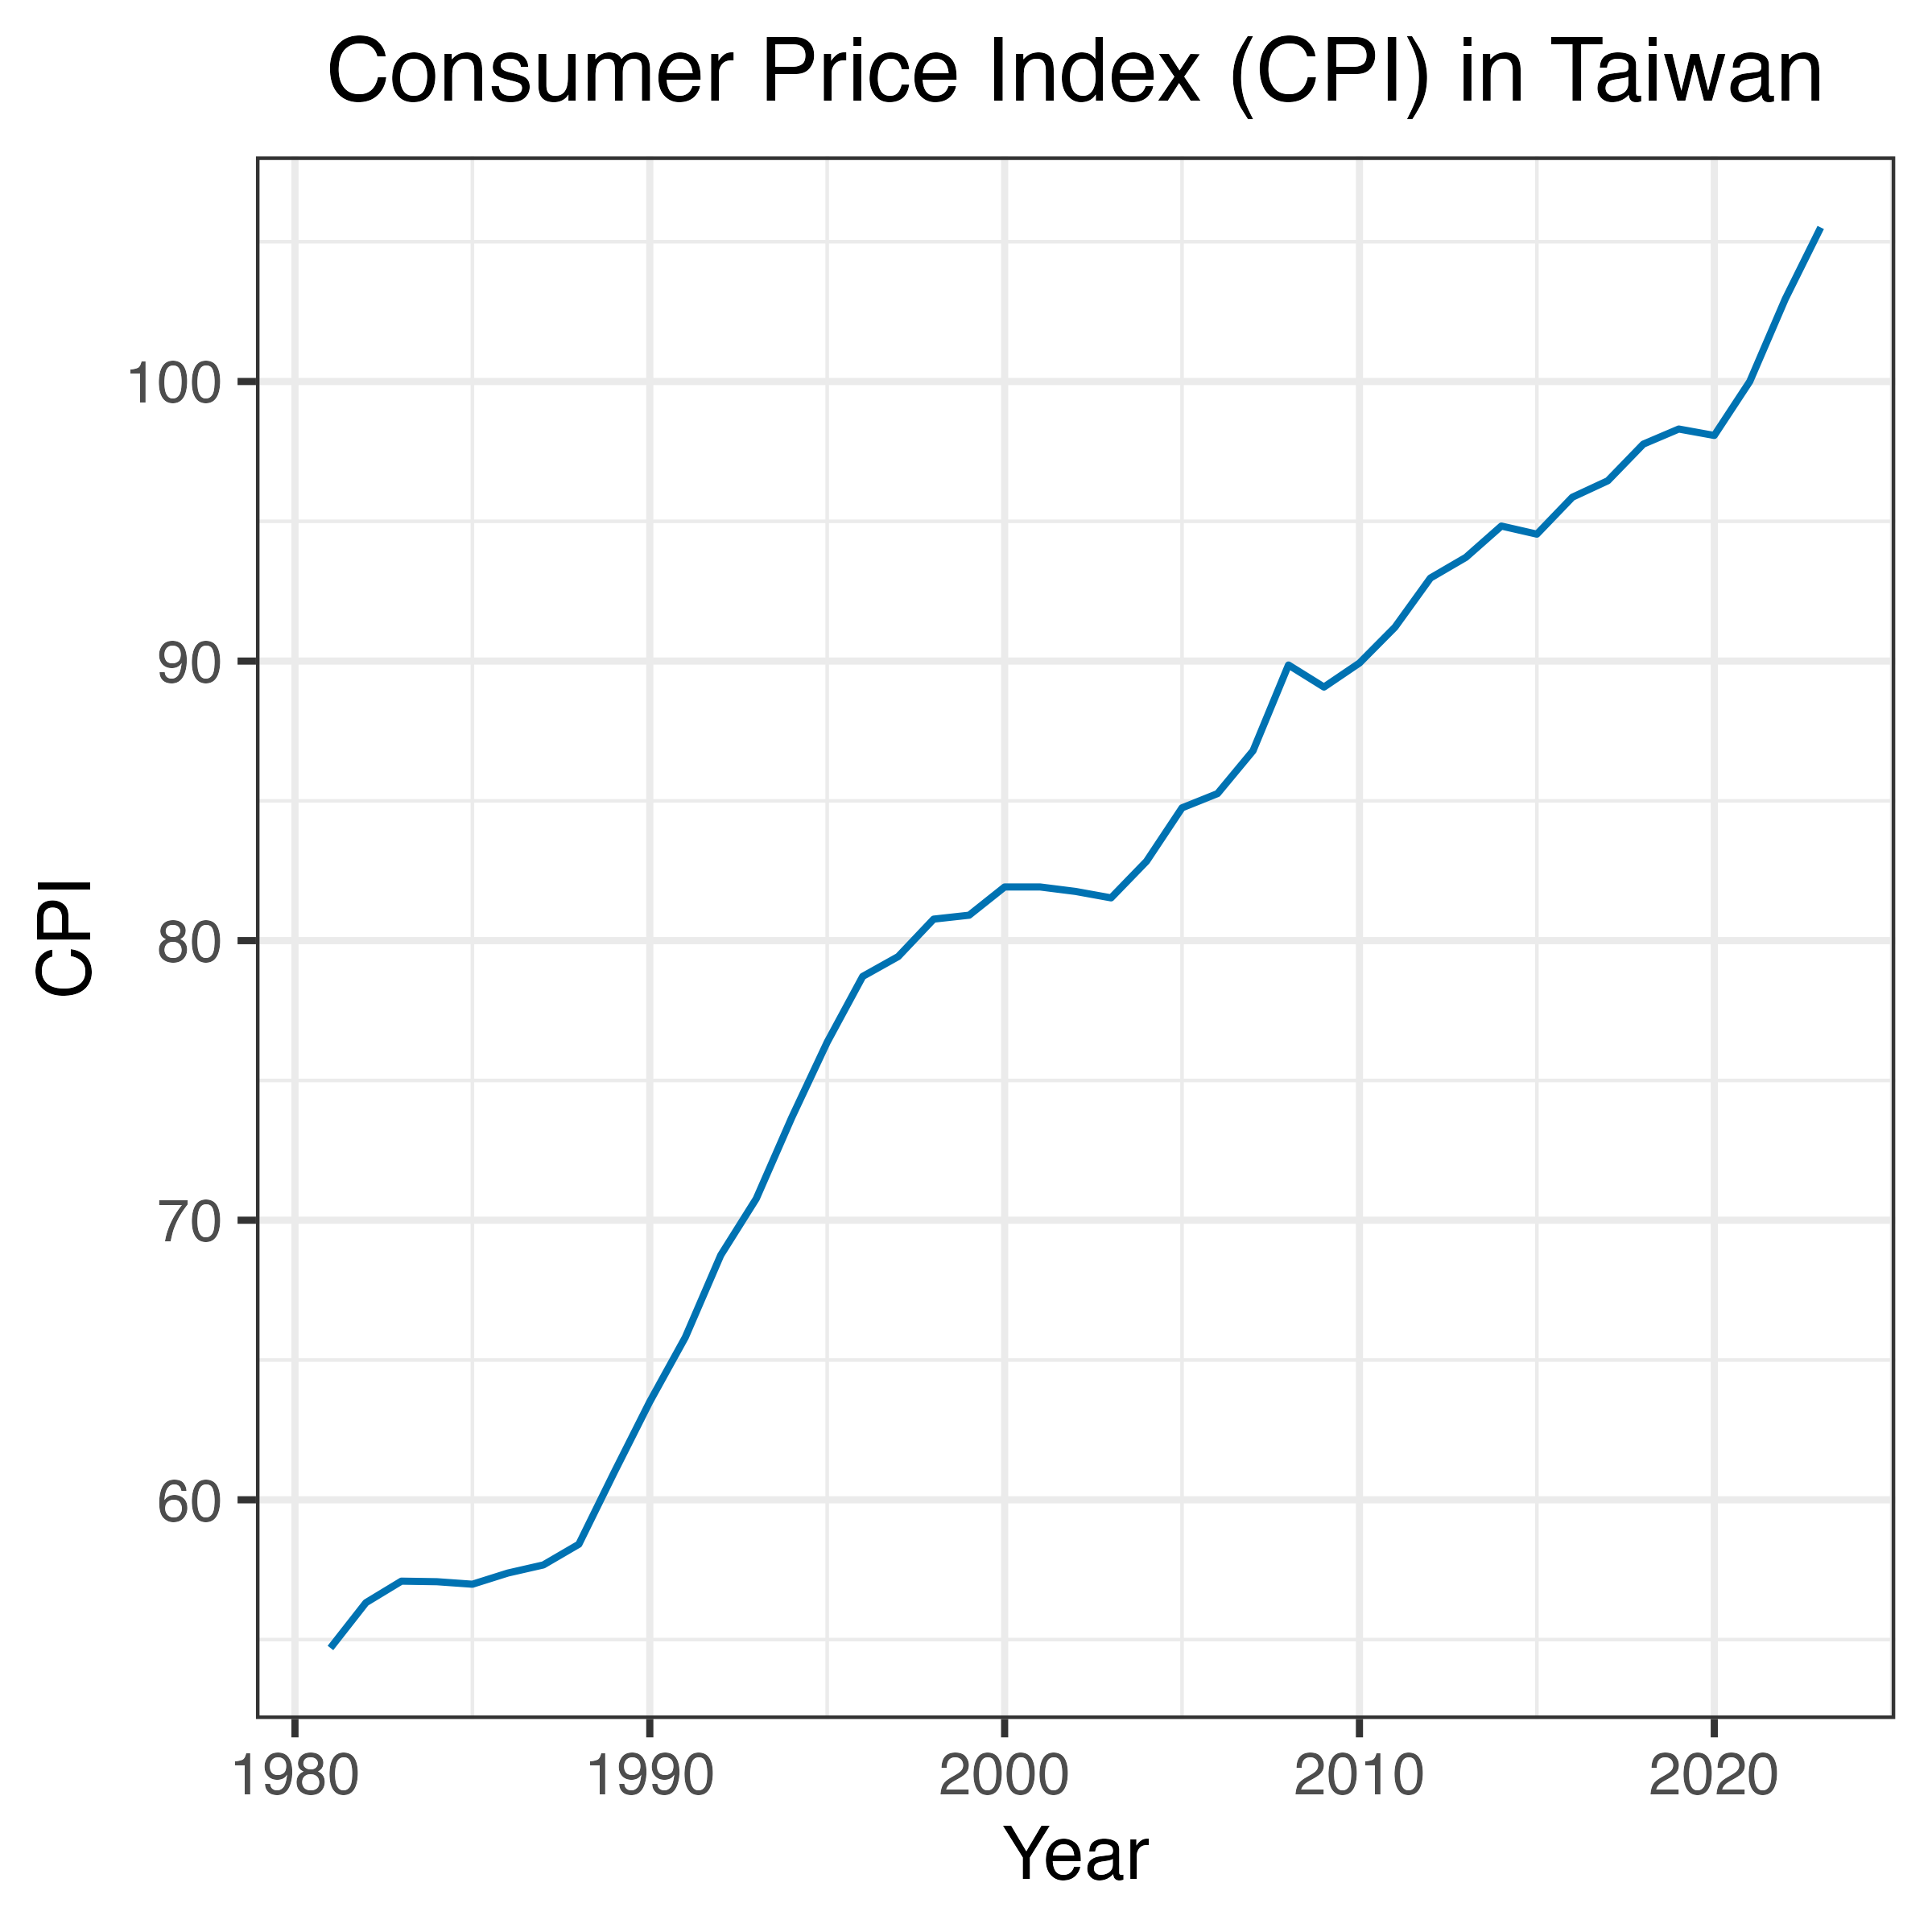
\includegraphics[width=0.45\textwidth]{figures/cpi.png}
    \caption{Consumer Price Index (CPI) in Taiwan, 1981 - 2023}
    \label{fig:CPI}
\end{figure}

\subsection{Equivalize Household Income and Consumption}

To compare households of different sizes and compositions, I use the OECD equivalence scale to adjust household income and consumption to per-adult-equivalent levels. 
The OECD scale assigns a weight of 1 to the first adult, 0.7 to each additional adult, and 0.5 to each child. 
I define a child as aged 17 or younger, while the original OECD definition is 13 or younger. 
The main earner's earnings are also divided by the household's weight, which gives the household's equivalized earnings if the main earner were its only earner. 
This places the main earner on the same scale as household earnings in Figure \ref{fig:Indi_to_HH}, so the gap reflects the earnings of other members rather than household size. 
Spouses' earnings are left on a per-earner basis. They enter only the two-earner share, which is a count, and the between-spouse correlation, where dividing both spouses by the same weight would raise the correlation mechanically.

\subsection{Sample Restrictions}
\label{sec:sample}

The sample is built in four steps, applied in this order.
\begin{enumerate}
    \item The 2012 survey year is excluded, since its income and expenditure values are all missing.
    \item When an income or expenditure is a sum or difference of survey items, such as household earnings as the sum of labor and industry earnings, a missing item is treated as zero.
    \item Each series of statistic is computed over households with a strictly positive value, so that every logarithm is defined. Zero, negative and missing values are excluded. This applies to every income and consumption statistics in the paper, following the design of Heathcote, Perri, \& Violante (\citeyear{HEATHCOTE_2010}).
    \item For measuring inequalities, households whose value falls below 5\% of that year's median are excluded. 
\end{enumerate}

Steps 3 and 4 are applied to one series at a time and are not carried into aggregates. 
Each aggregate is first summed from its components in step 2, before anything is excluded, steps 3 and 4 are then applied to the aggregate itself. 
For example, a household with no earnings or with earnings below the floor is left out of every statistic on household earnings. 
If it has asset income, however, it stays in the statistics on total income, provided that its total income passes the threshold. 
As a result, the statistics compared within one figure can cover different households.

Step 4 is needed because the two main dispersion measures in this paper react very differently to values close to zero. 
A household with small positive earnings contributes a logarithm far below the mean, which raises the variance of logs substantially. 
In contrast, the Gini coefficient is calculated from the Lorenz curve, so a few households with very low earnings have little effect on it.
Such households are rare early in the sample but become much more common after 2015, especially in the pandemic years. 
Without step 4, the variance of log household earnings more than triples between 1981 and 2023, from 0.29 to 0.97. With it, the variance rises only from 0.28 to 0.48. 
Appendix \ref{sec:appendix_sample} compares the sample of each series with and without the threshold.

Excluding observations close to zero is common practice when dispersion is measured in logarithms. Heathcote, Perri, and Violante (\citeyear{HEATHCOTE_2010}) exclude households with non-positive earnings and then the bottom 0.5\% of the remaining distribution, reapplying the trim to each definition of income, because the variance of logs is very sensitive to realizations close to zero. 
Guvenen, Pistaferri, and Violante (\citeyear{GRID_2022}) drop earnings below a threshold tied to the minimum wage, so that records of workers without a meaningful attachment to the labor force do not skew log-based statistics. 
The Luxembourg Income Study bottom-coded incomes at 1\% of mean equivalized household income (Neugschwender, \citeyear{LIS_coding}). 
In this paper, I drop observations below 5\% of the median rather than a fixed share of each year's sample. 
The share of households near zero grows from about 0.1\% in the early 1980s to around 2\% in 2018, so a fixed share cannot remove them in every year. Trimming the bottom 0.5\% each year, as Heathcote, Perri, and Violante (\citeyear{HEATHCOTE_2010}) do, leaves the 2023 variance at 0.69, against 0.48 under the 5\% median threshold.

\section{Household-level Inequality}
\label{sec:household_inequality}

Here, I present the household-level inequality measures, including earnings and consumption inequality, and their cyclical dynamics. This paper skips individual-level inequality, which is better estimated from tax records. Individual-level consumption is not available in the SFIE, as it only records household-level non-durable consumption.
Estimating consumption inequality using household-level data is also more suitable, as households can share consumption goods and services, such as housing and food, which are not easily separable at the individual level.
In this section, I follow the structure of Heathcote, Perri, and Violante (\citeyear{HEATHCOTE_2010}) to construct a complete picture of household-level inequality from basic earnings to disposable income and consumption. 


\subsection{Inequality in Earnings}

\begin{figure}
    \centering
    \begin{subfigure}[t]{0.475\textwidth}
        \centering
        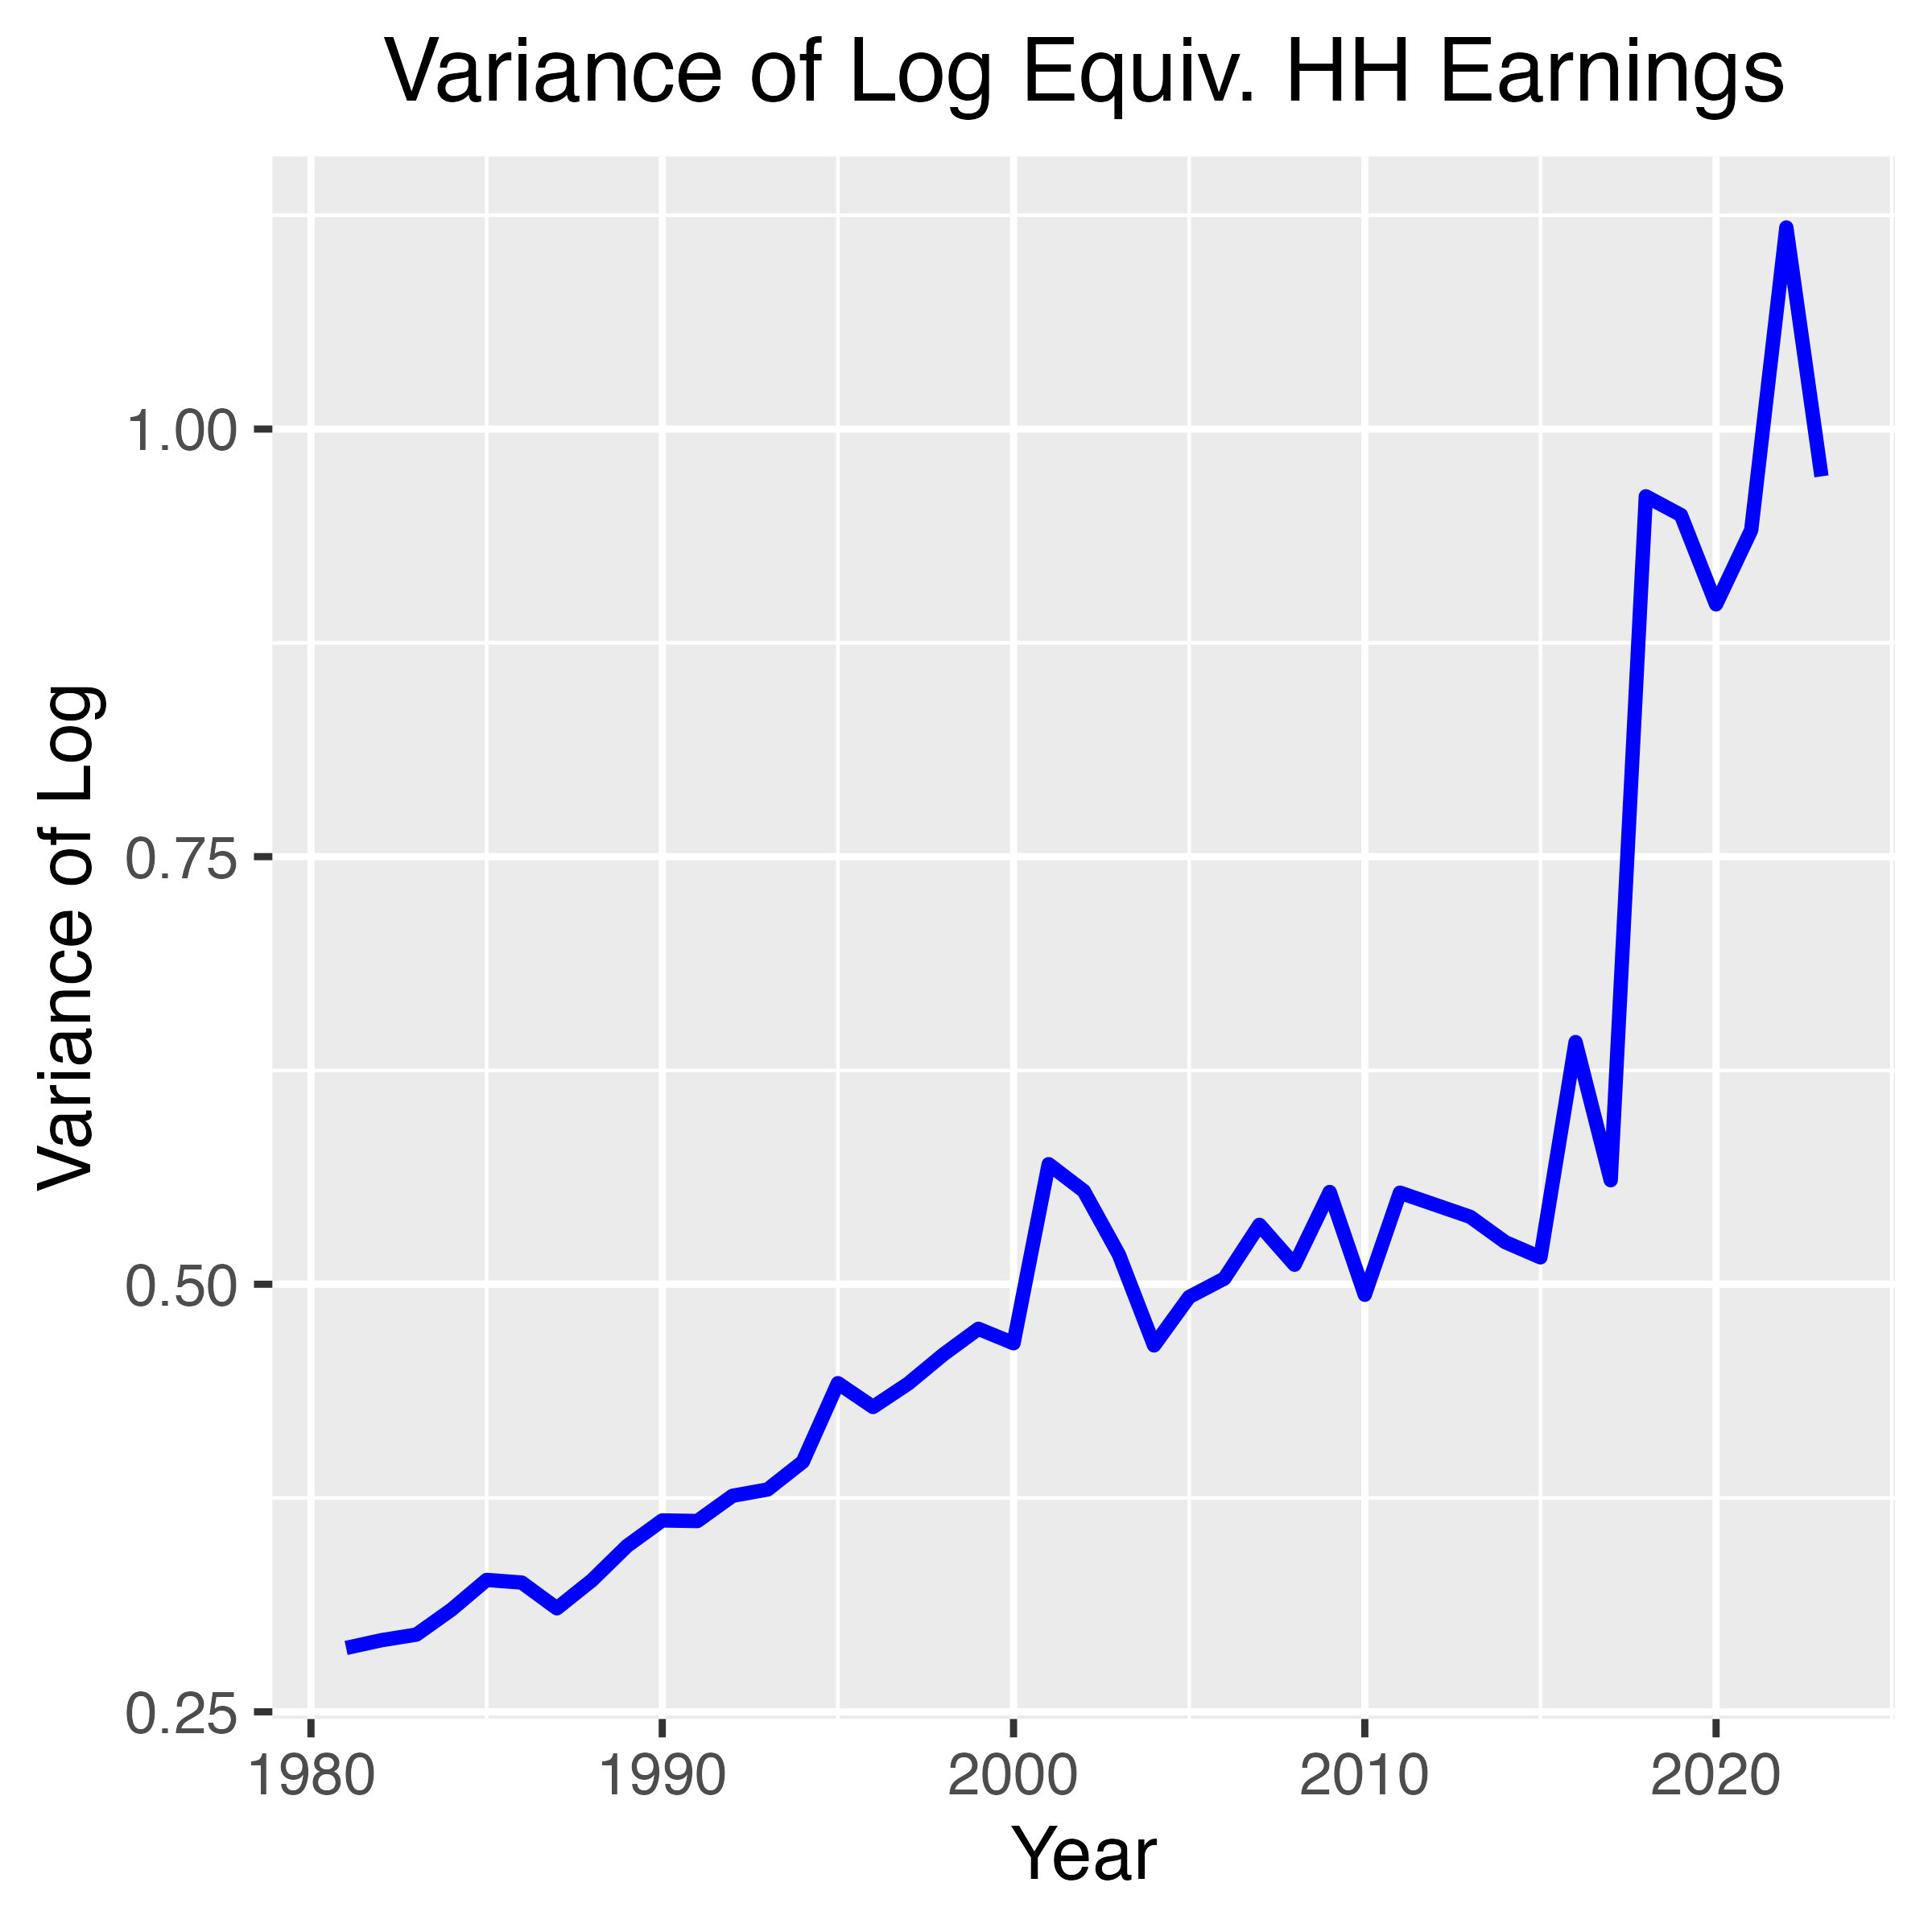
\includegraphics[width=\textwidth]{figures/Fig_1/Fig_1a_Var_Earnings.png}
    \end{subfigure}
    \begin{subfigure}[t]{0.475\textwidth}
        \centering
        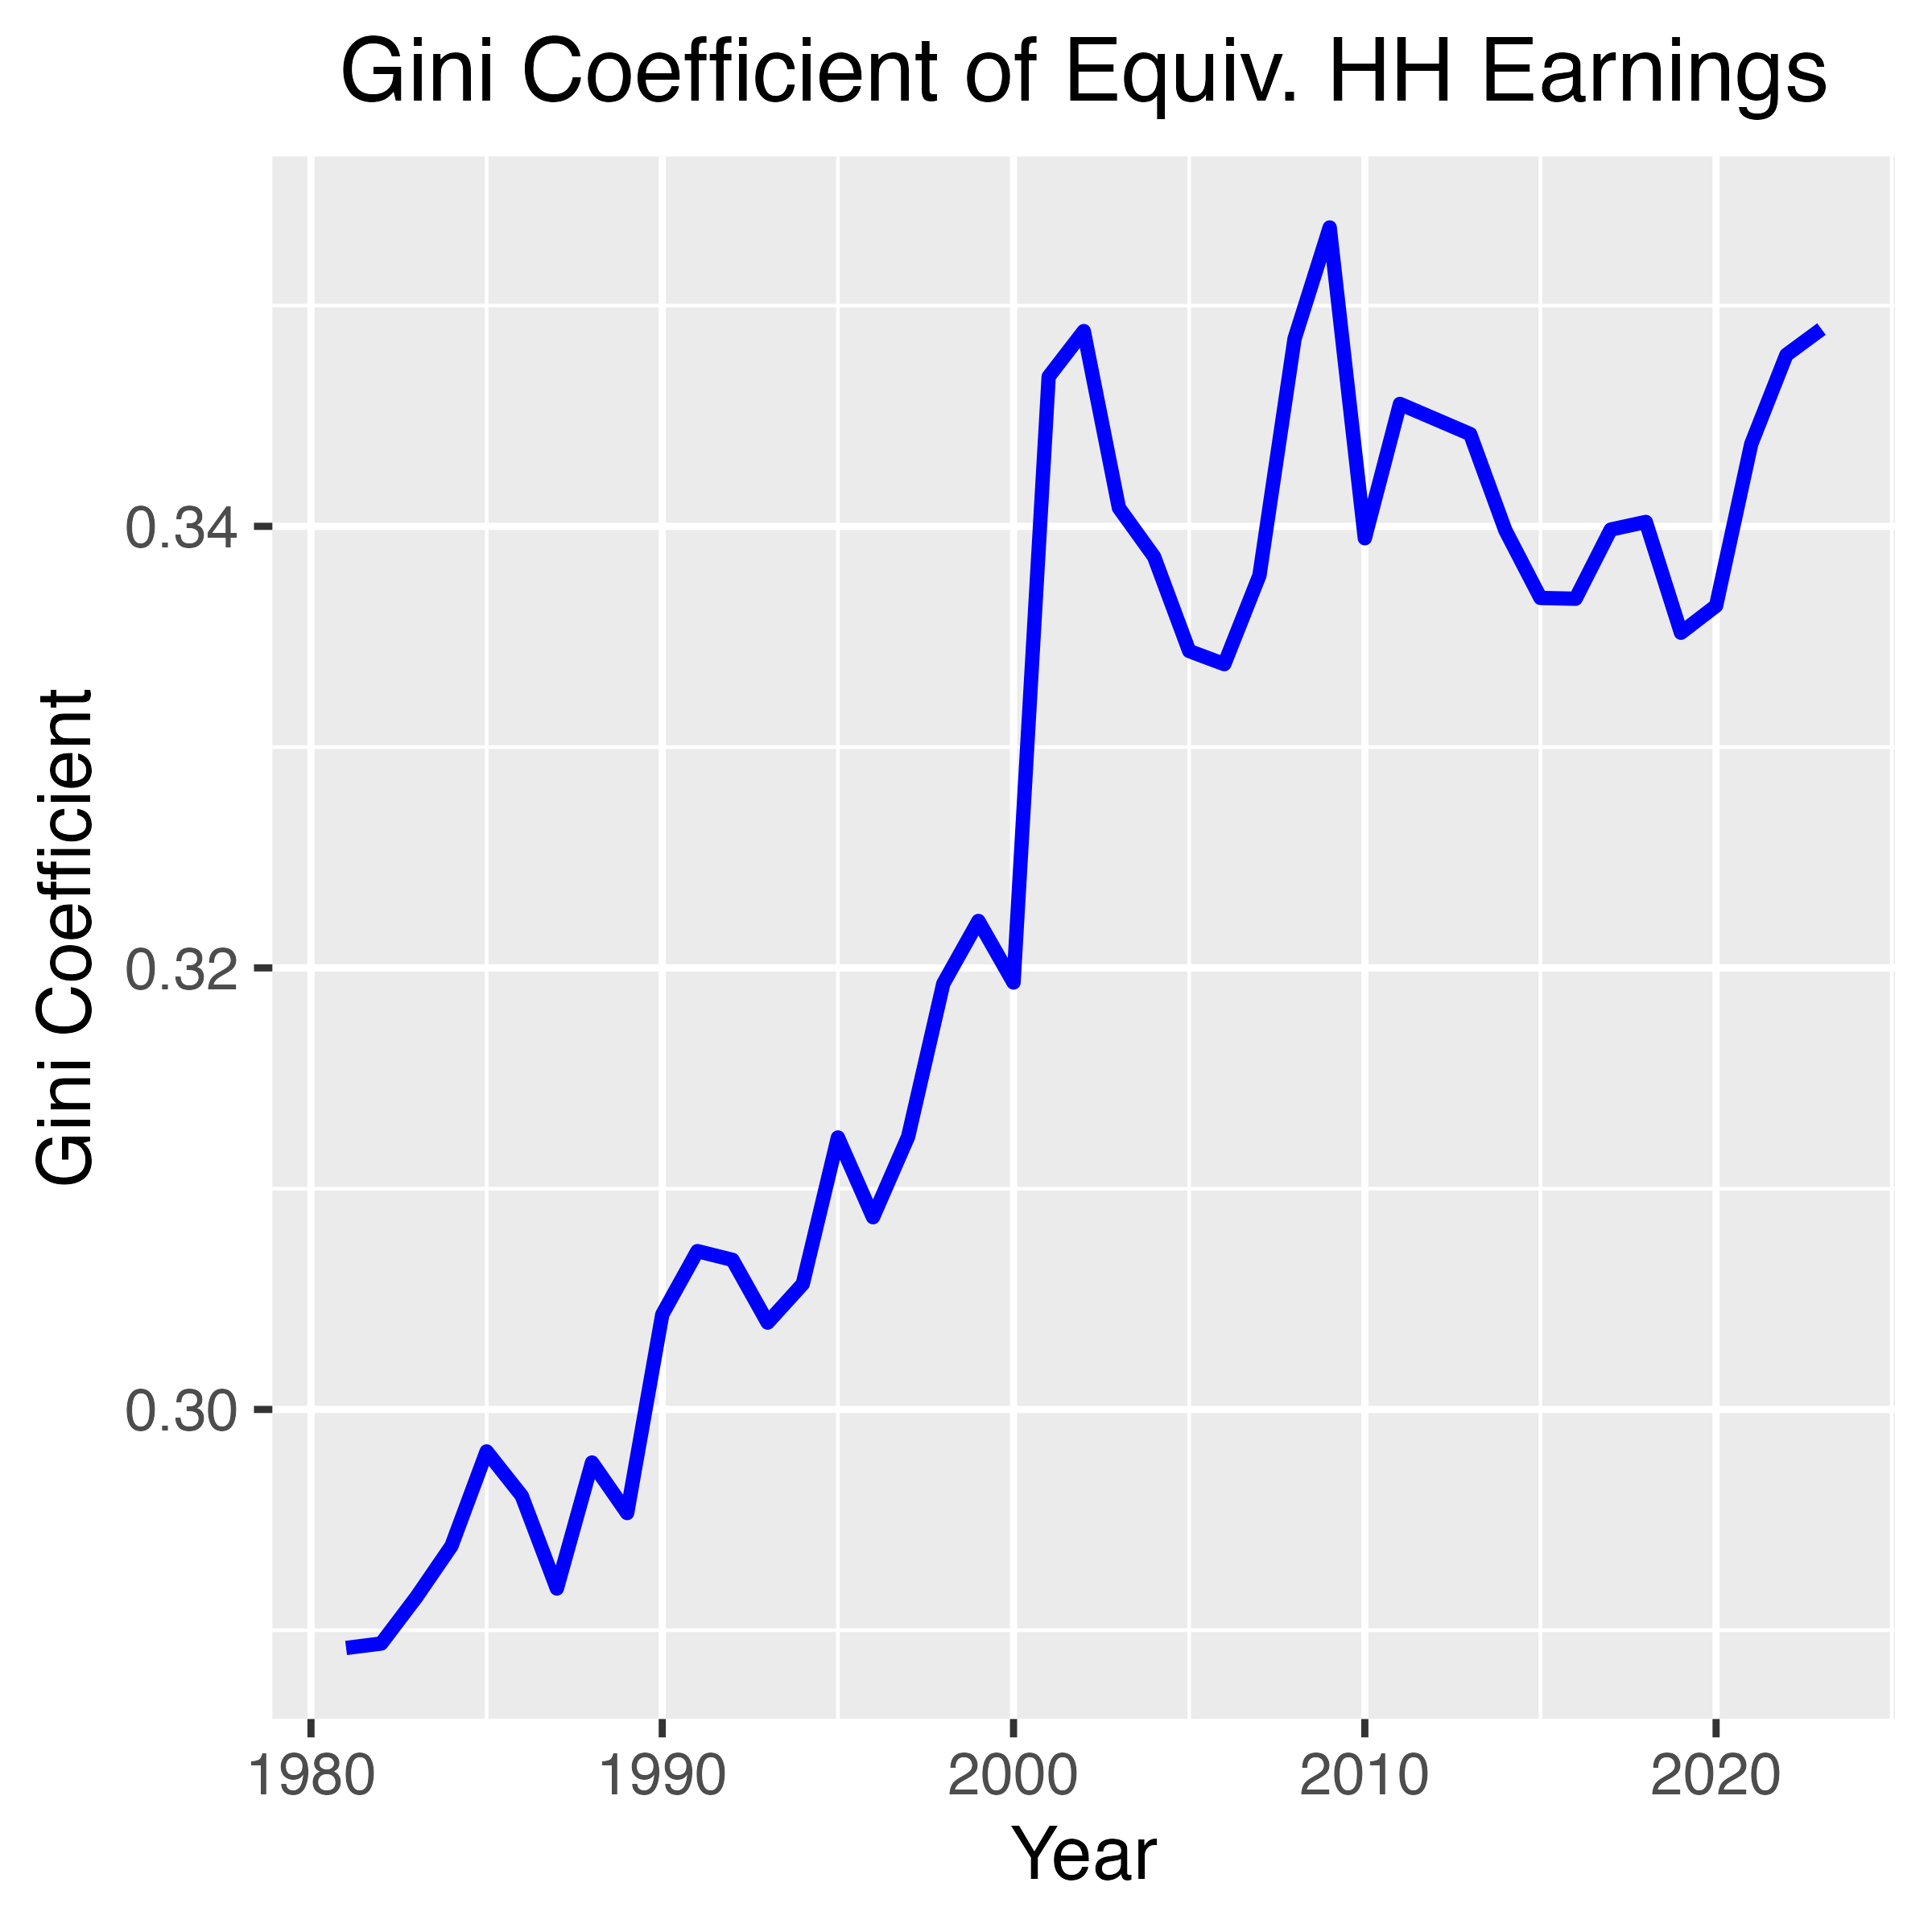
\includegraphics[width=\textwidth]{figures/Fig_1/Fig_1b_Gini_Earnings.png}
    \end{subfigure}
    \begin{subfigure}[t]{0.475\textwidth}
        \centering
        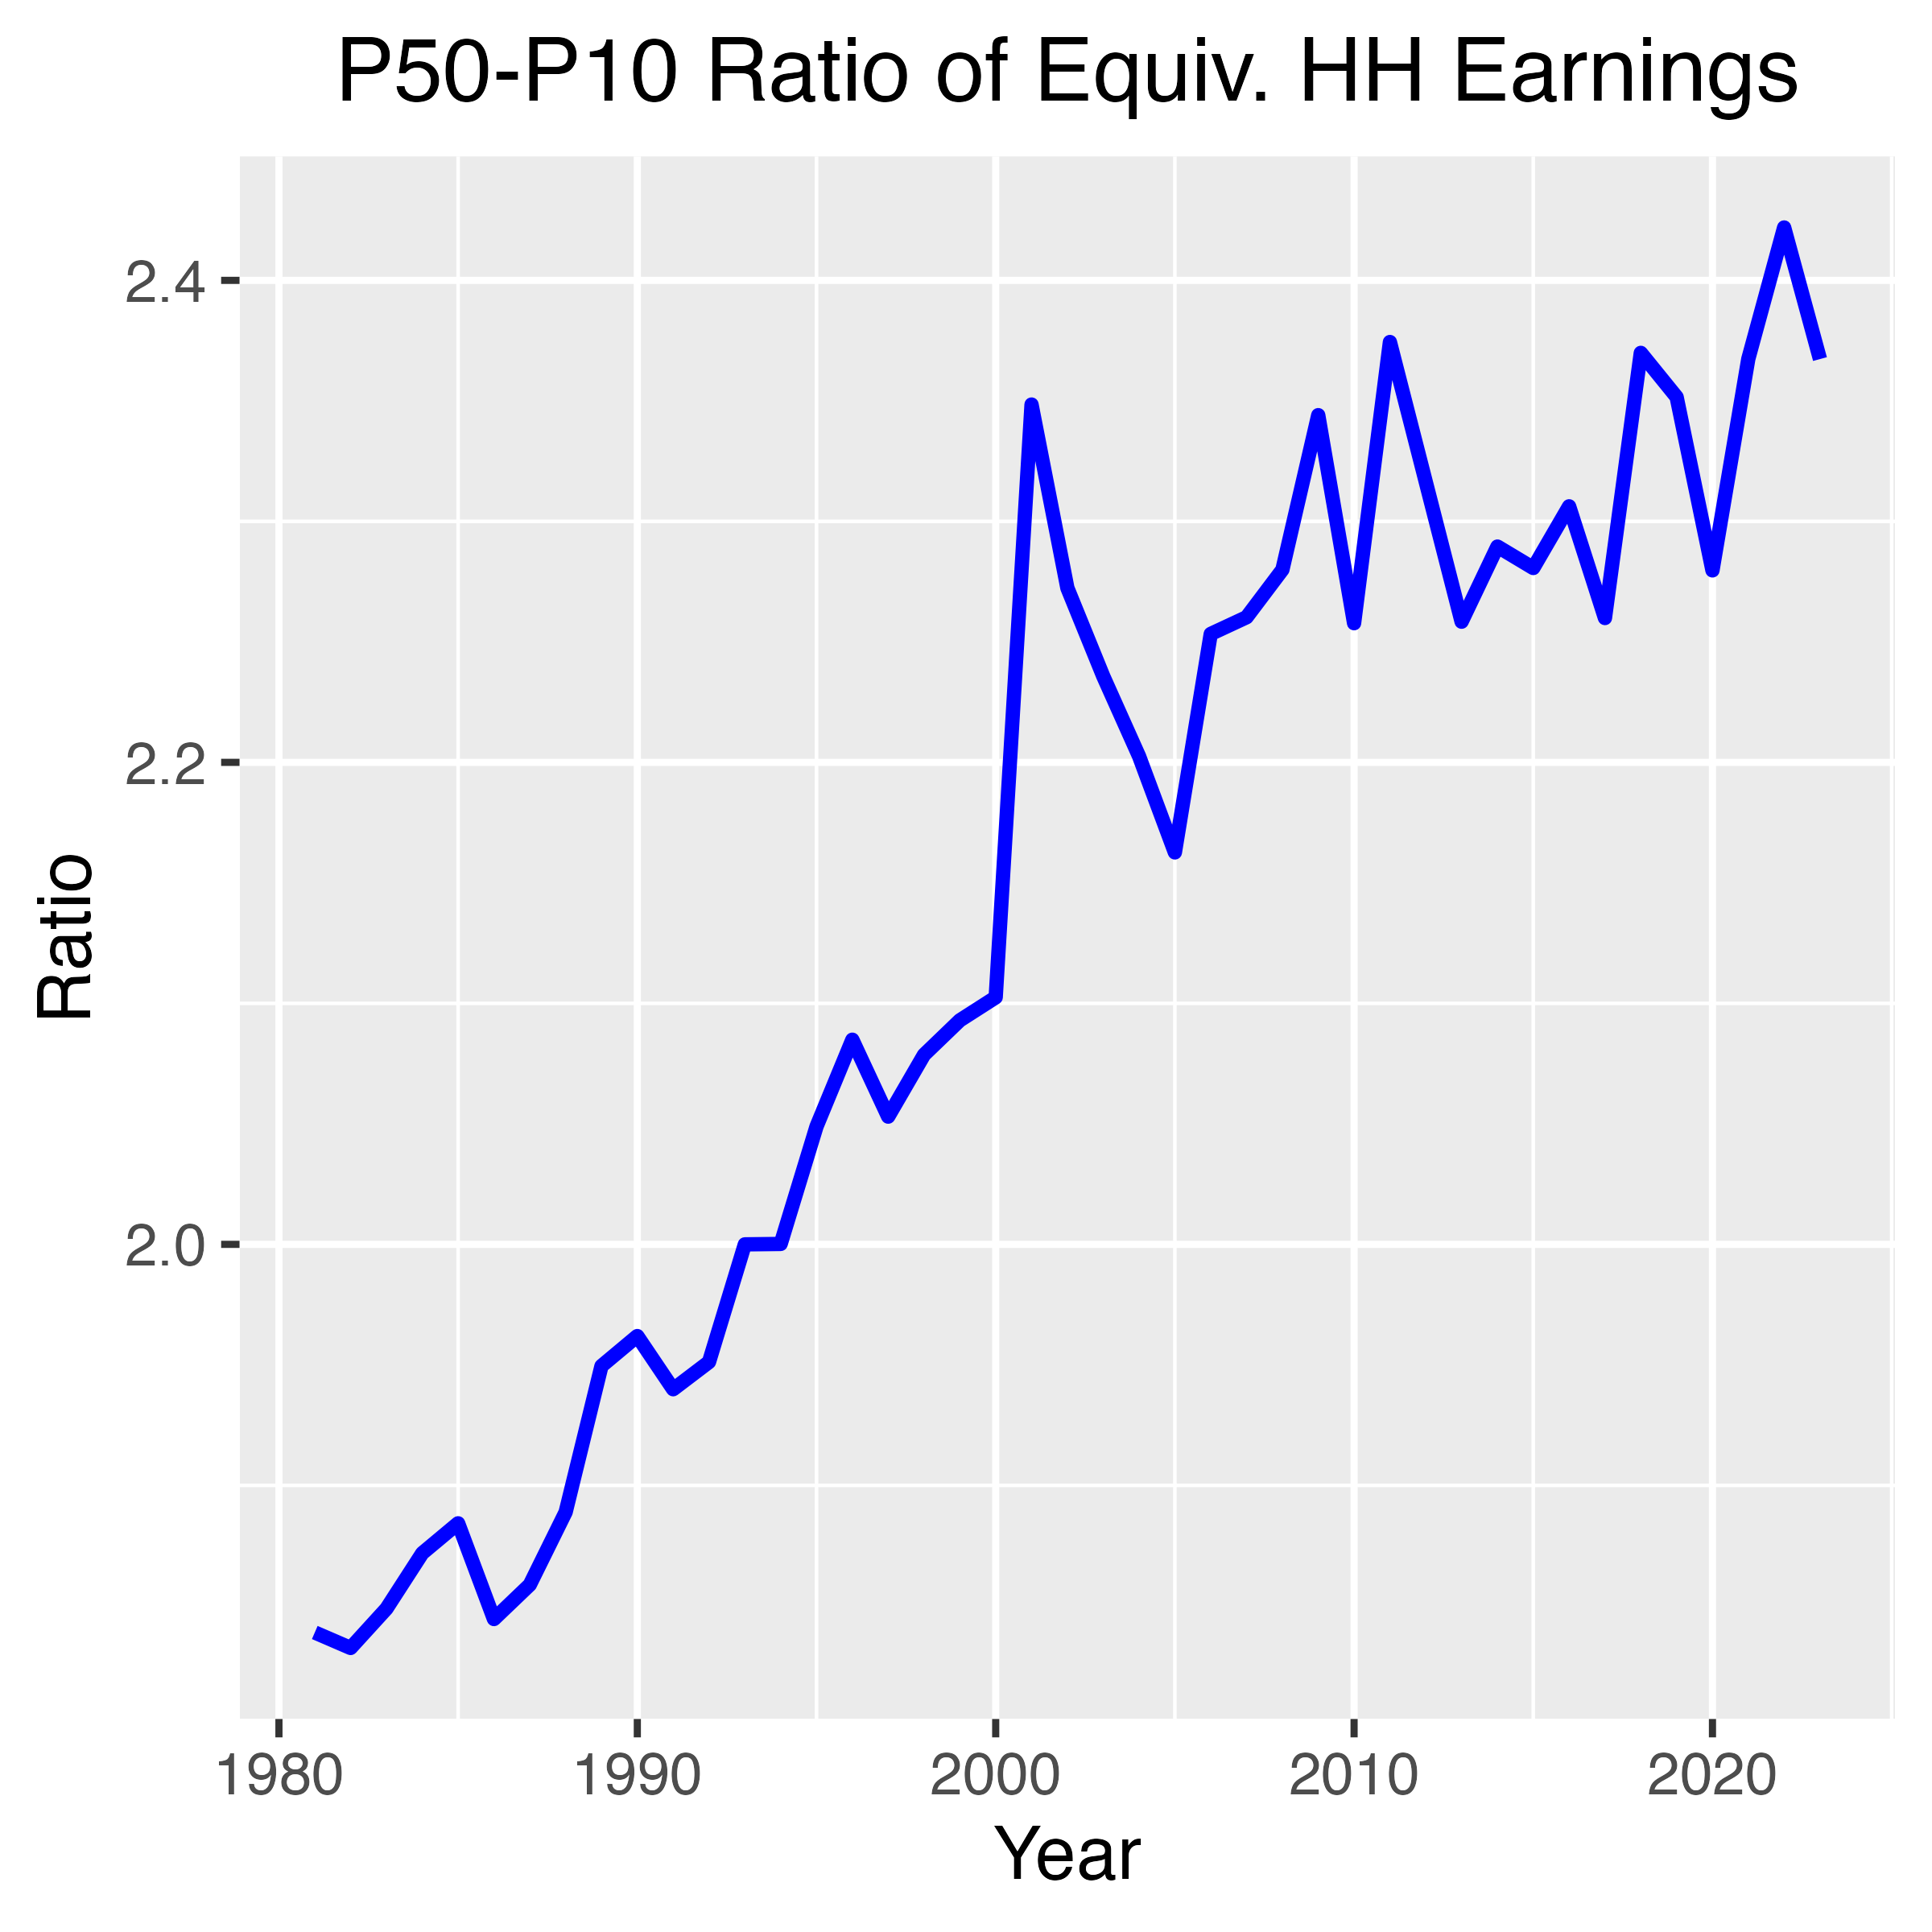
\includegraphics[width=\textwidth]{figures/Fig_1/Fig_1c_P50_P10_Earnings.png}
    \end{subfigure}
    \begin{subfigure}[t]{0.475\textwidth}
        \centering
        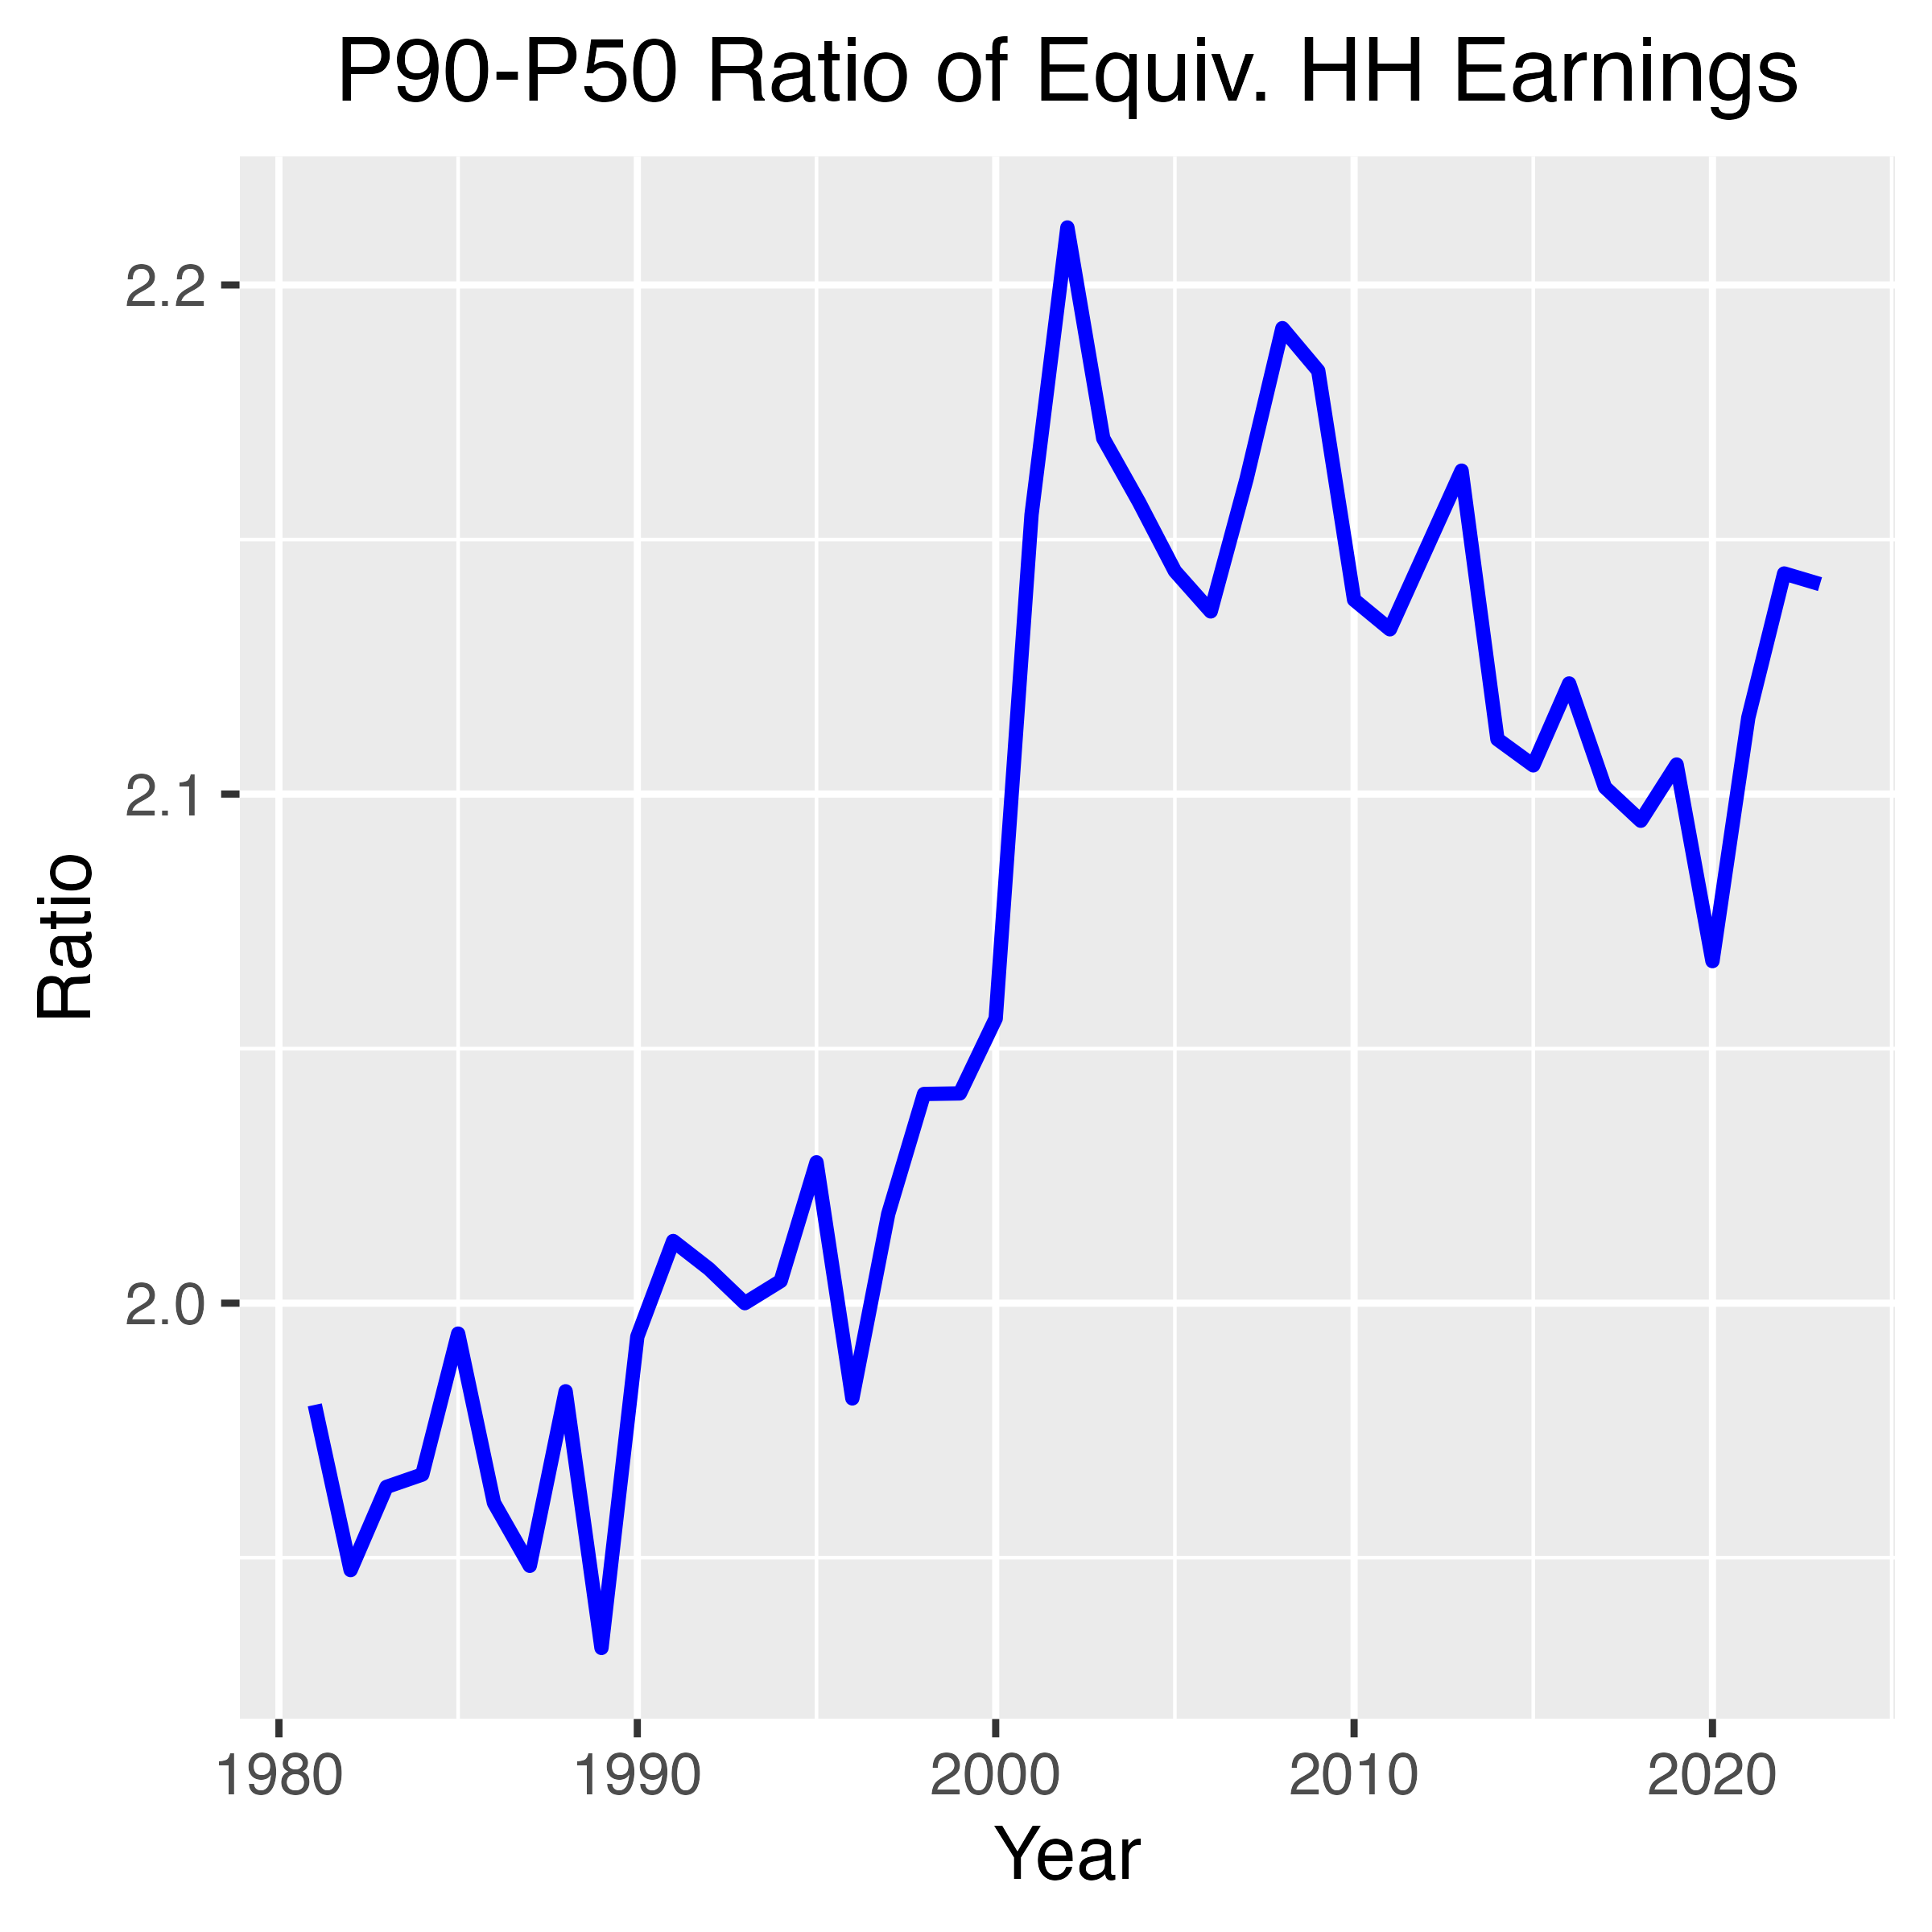
\includegraphics[width=\textwidth]{figures/Fig_1/Fig_1d_P90_P50_Earnings.png}
    \end{subfigure}
    \caption{Various Measures of Household Earnings Inequality}
    \label{fig:earnings_inequality}
\end{figure}

\begin{figure}
    \centering
    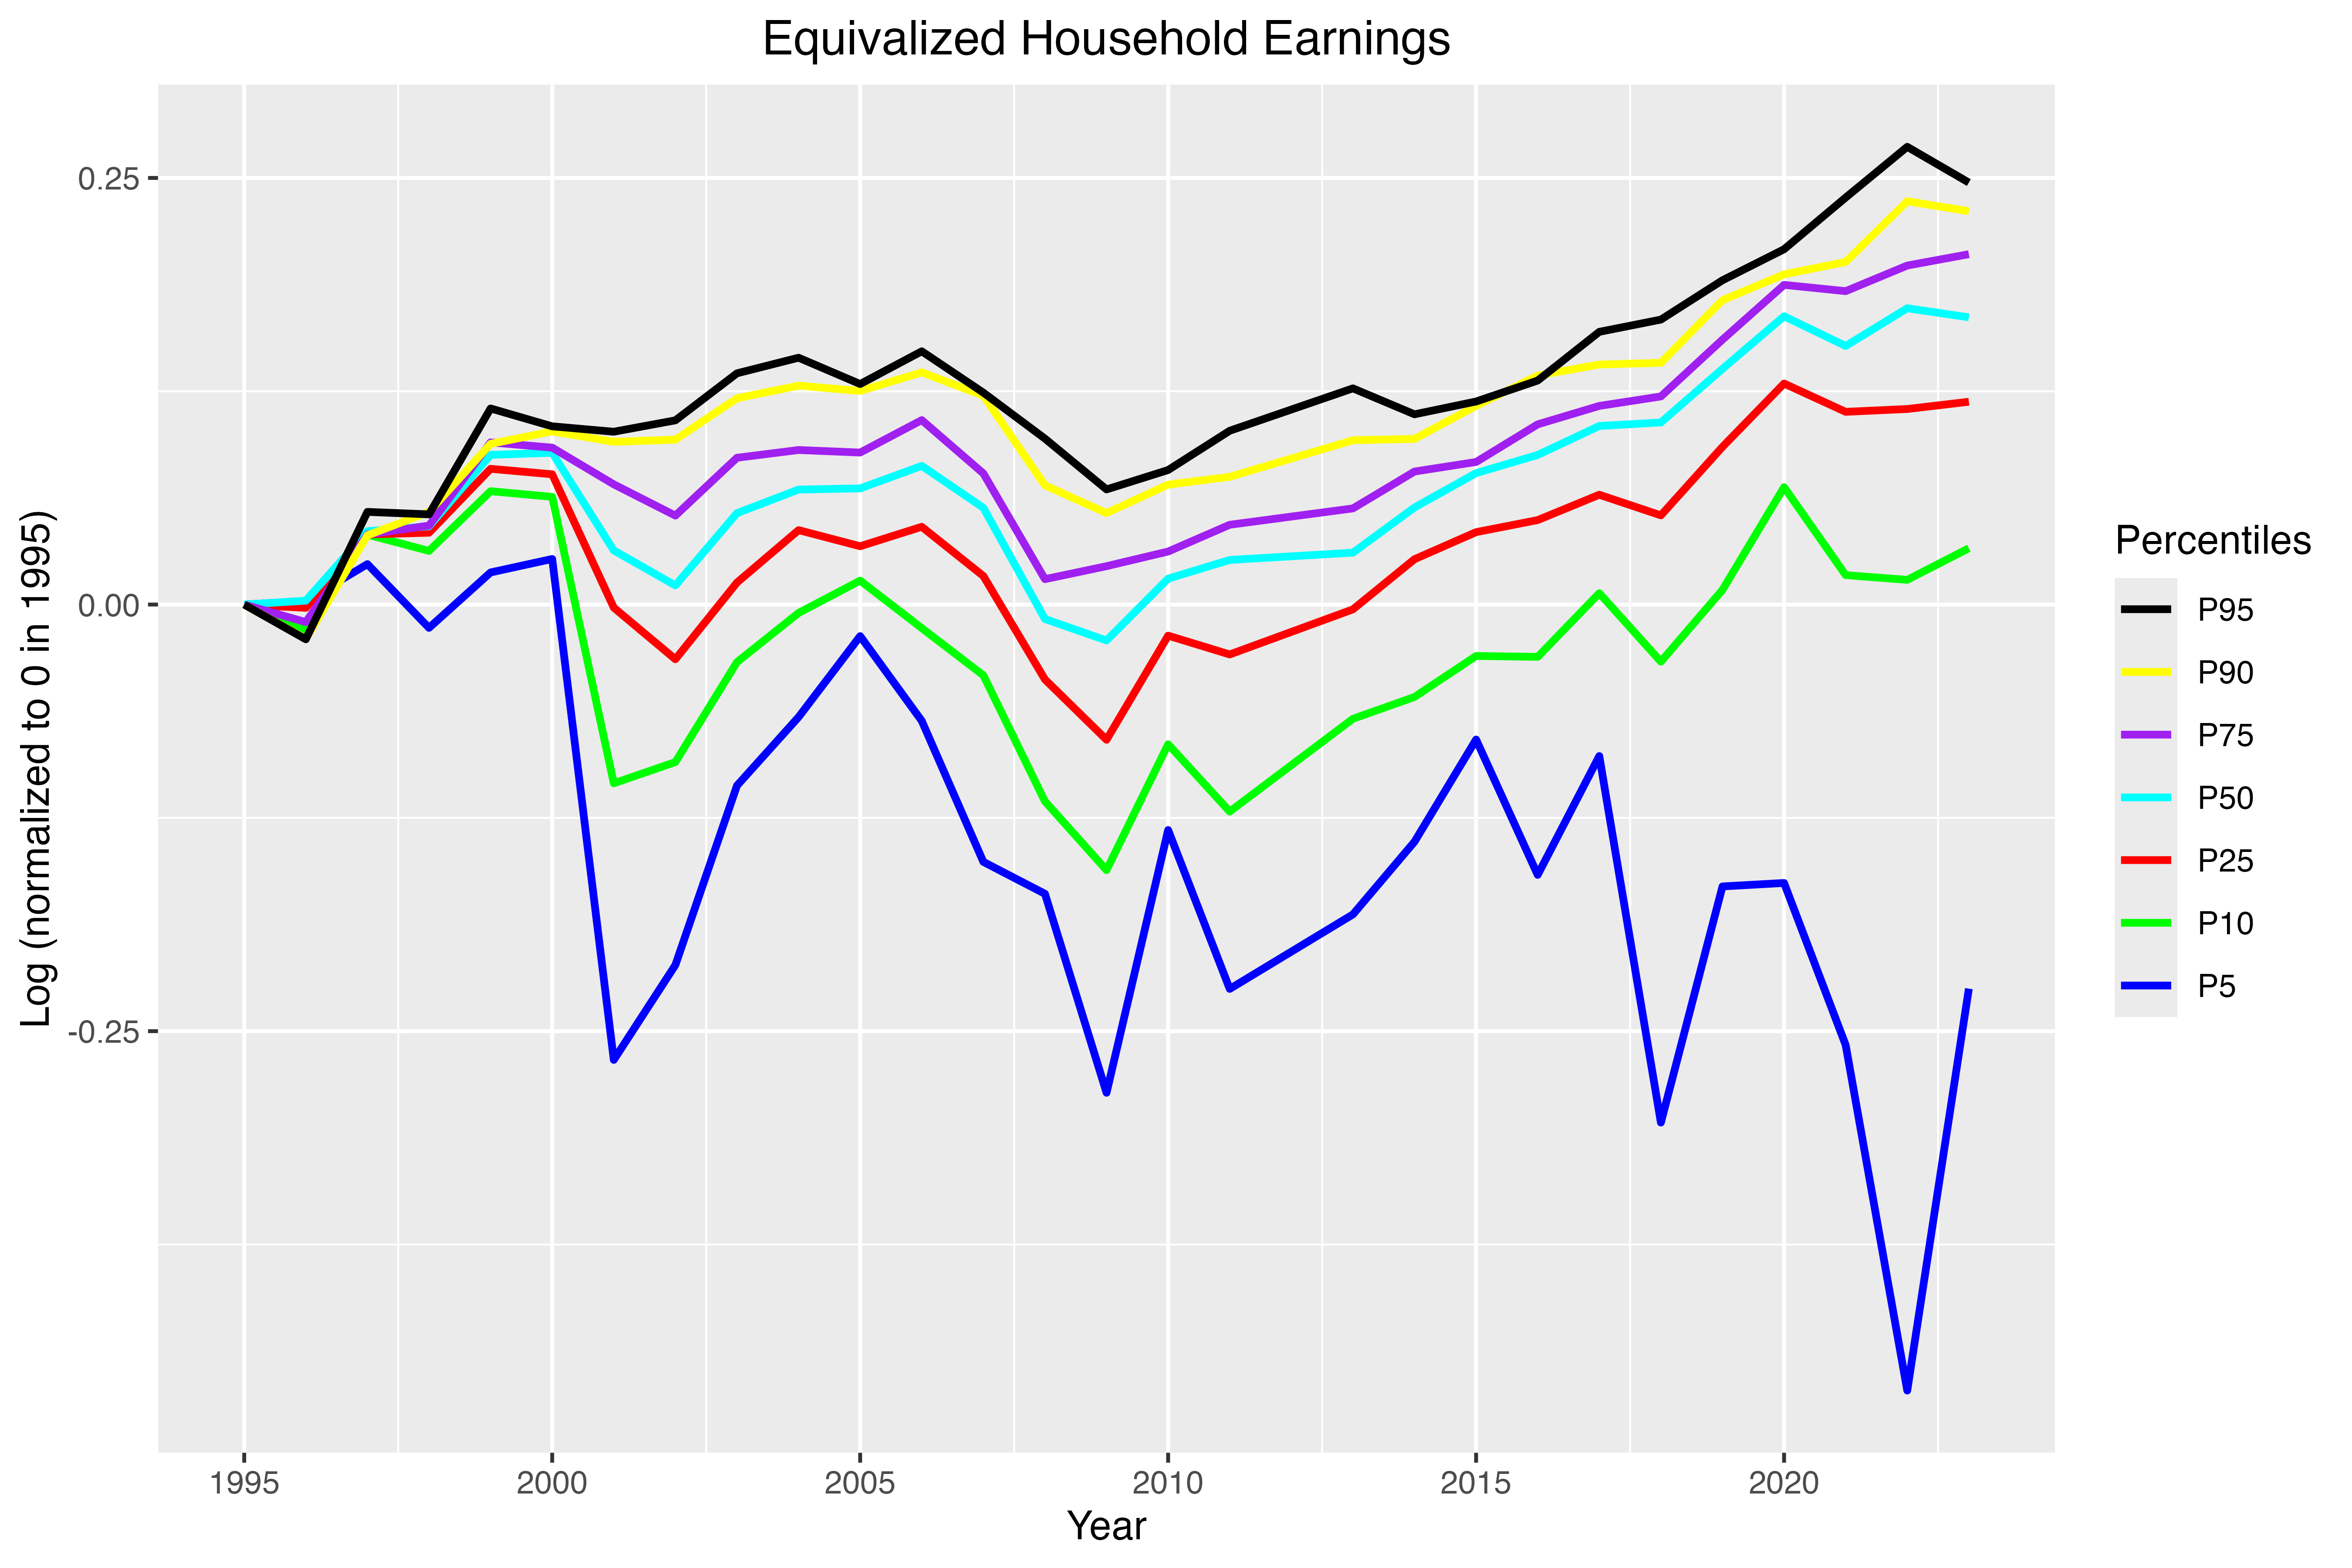
\includegraphics[width=0.95\textwidth]{figures/Fig_2/Fig_2_percentiles_a1995.png}
    \caption{Percentiles of the Household Earnings Distribution}
    \label{fig:earnings_inequality_cyclic}
\end{figure}

Figure \ref{fig:earnings_inequality} plots four measures of dispersion in household earnings: the variance of logs, the Gini coefficient, the P50-P10 ratio, and the P90-P50 ratio.
Though all measures of dispersion have increased since 1981, there are some minor differences in their dynamics.
The variance, the Gini coefficient, and the P50-P10 ratio track each other extremely closely. All three jump in 2001 after the Dot-com bubble and spike again in 2009 after the Global Financial Crisis. Since 2001 they have moved within a narrow band, the variance between 0.43 and 0.50 and the P50-P10 ratio between 2.12 and 2.31.
The Gini coefficient in the top right panel rises from 0.29 in 1981 to 0.35 in 2023, indicating that earnings inequality has risen over the past four decades. Almost all of that rise happens by 2001. After 2001, the Gini has stayed between 0.33 and 0.35.
The P90-P50 ratio is the most interesting one. It also spikes around the Dot-com bubble, peaking at 2.21 in 2002, and then falls back to 2.07 by 2020, a stretch over which the top decile grew more slowly than the median. It climbs again to 2.14 by 2023, recovering half of that decline, so the compression at the top is at least partly an episode rather than a trend.
It is worth noting that though the dispersion of earnings appears to rise steeply in Figure \ref{fig:earnings_inequality}, the rise is moderate in size. The Gini increases by only 0.06 between 1981 and 2023. The variance of logs increases by 0.16 between 1981 and 2006 and by 0.20 by 2023. Heathcote, Perri, and Violante (\citeyear{HEATHCOTE_2010}) find that in the US the variance of log equivalized household earnings rises by roughly 0.30 from 1967 to the early 1990s, also about 25 years, and then levels off. Over its first 25 years, Taiwan's variance therefore rises by about half as much as the US variance. 

\subsection{Cyclical Dynamics of Earnings Inequality}

Figure \ref{fig:earnings_inequality_cyclic} shows the trend in percentiles at different points in the distribution of household earnings from 1995 to 2023. Log earnings are normalized to 0 in 1995, so the y-axis shows the change in earnings relative to 1995 in log points.
Here, I show only the years from 1995 onward. The full series from 1981 to 2023 are in Appendix \ref{sec:appendix_cyclical_dynamics}, normalized to 1981 in Figure \ref{fig:appendix_cyclic_earnings_1981} and to 1995 in Figure \ref{fig:appendix_cyclic_earnings_1995}. 
The reason for this choice is that every percentile grew by between 79 and 102 log points from 1981 to 1995. That is, earnings at every point of the distribution more than doubled in fourteen years.
This finding is consistent with Bourguignon, Fournier, and Gurgand (\citeyear{TW_stable_dist}), who find that before 1994 Taiwan developed fast while its income distribution stayed stable.
Therefore, putting years before 1995 in the main figure could dilute the interpretation of recent trends, as the rapid growth phase would dominate the visual impression. By focusing on the period after 1995, we can better highlight the cyclical and structural changes in earnings inequality that occurred after Taiwan's high-growth era ended. This approach allows for a more precise analysis of the dynamics relevant to the current policy and economic environment.

We can see the fanning out of the earnings distribution over time: the lower the percentile, the less it grew. From 1995 to 2023 the bottom 5\% gained about 5 log points, against 18 for the median. P5 moves in a sequence of troughs, about 19 log points below its 1995 level in 2001 after the Dot-com bubble, and 25 below it in 2009 after the Global Financial Crisis. It then recovers steadily to 9 log points above its 1995 level in 2020, falls by 12 log points in 2021, during the COVID-19 pandemic, and is back at 5 above it in 2023. The pandemic decline at the bottom is therefore smaller and shorter-lived than the two before it.
In contrast, growth across the top half of the distribution is tightly bunched. The median has gained about 18 log points since 1995, the 90th percentile 24 and the 95th 25. The divergence in Figure \ref{fig:earnings_inequality} is therefore between the top half and the bottom half, not within the top half.

Inequality tends to widen during recessions, such as after the Dot-com bubble in 2001, the Global Financial Crisis in 2008 and 2009, and during the COVID-19 pandemic in 2021 and 2022. The reason behind this phenomenon is that when facing external shocks, households with higher earnings are more likely to have diversified income sources, such as investments and insurance transfers, which can help them absorb shocks better than those with lower earnings who rely more on labor income. We can also observe this phenomenon in the percentiles of earnings distribution, where the lower percentiles tend to decline sharply while the upper percentiles remain relatively stable during recessions.

\subsection{From Individual to Household Inequality}

\begin{figure}
    \centering
    \begin{subfigure}[t]{0.475\textwidth}
        \centering
        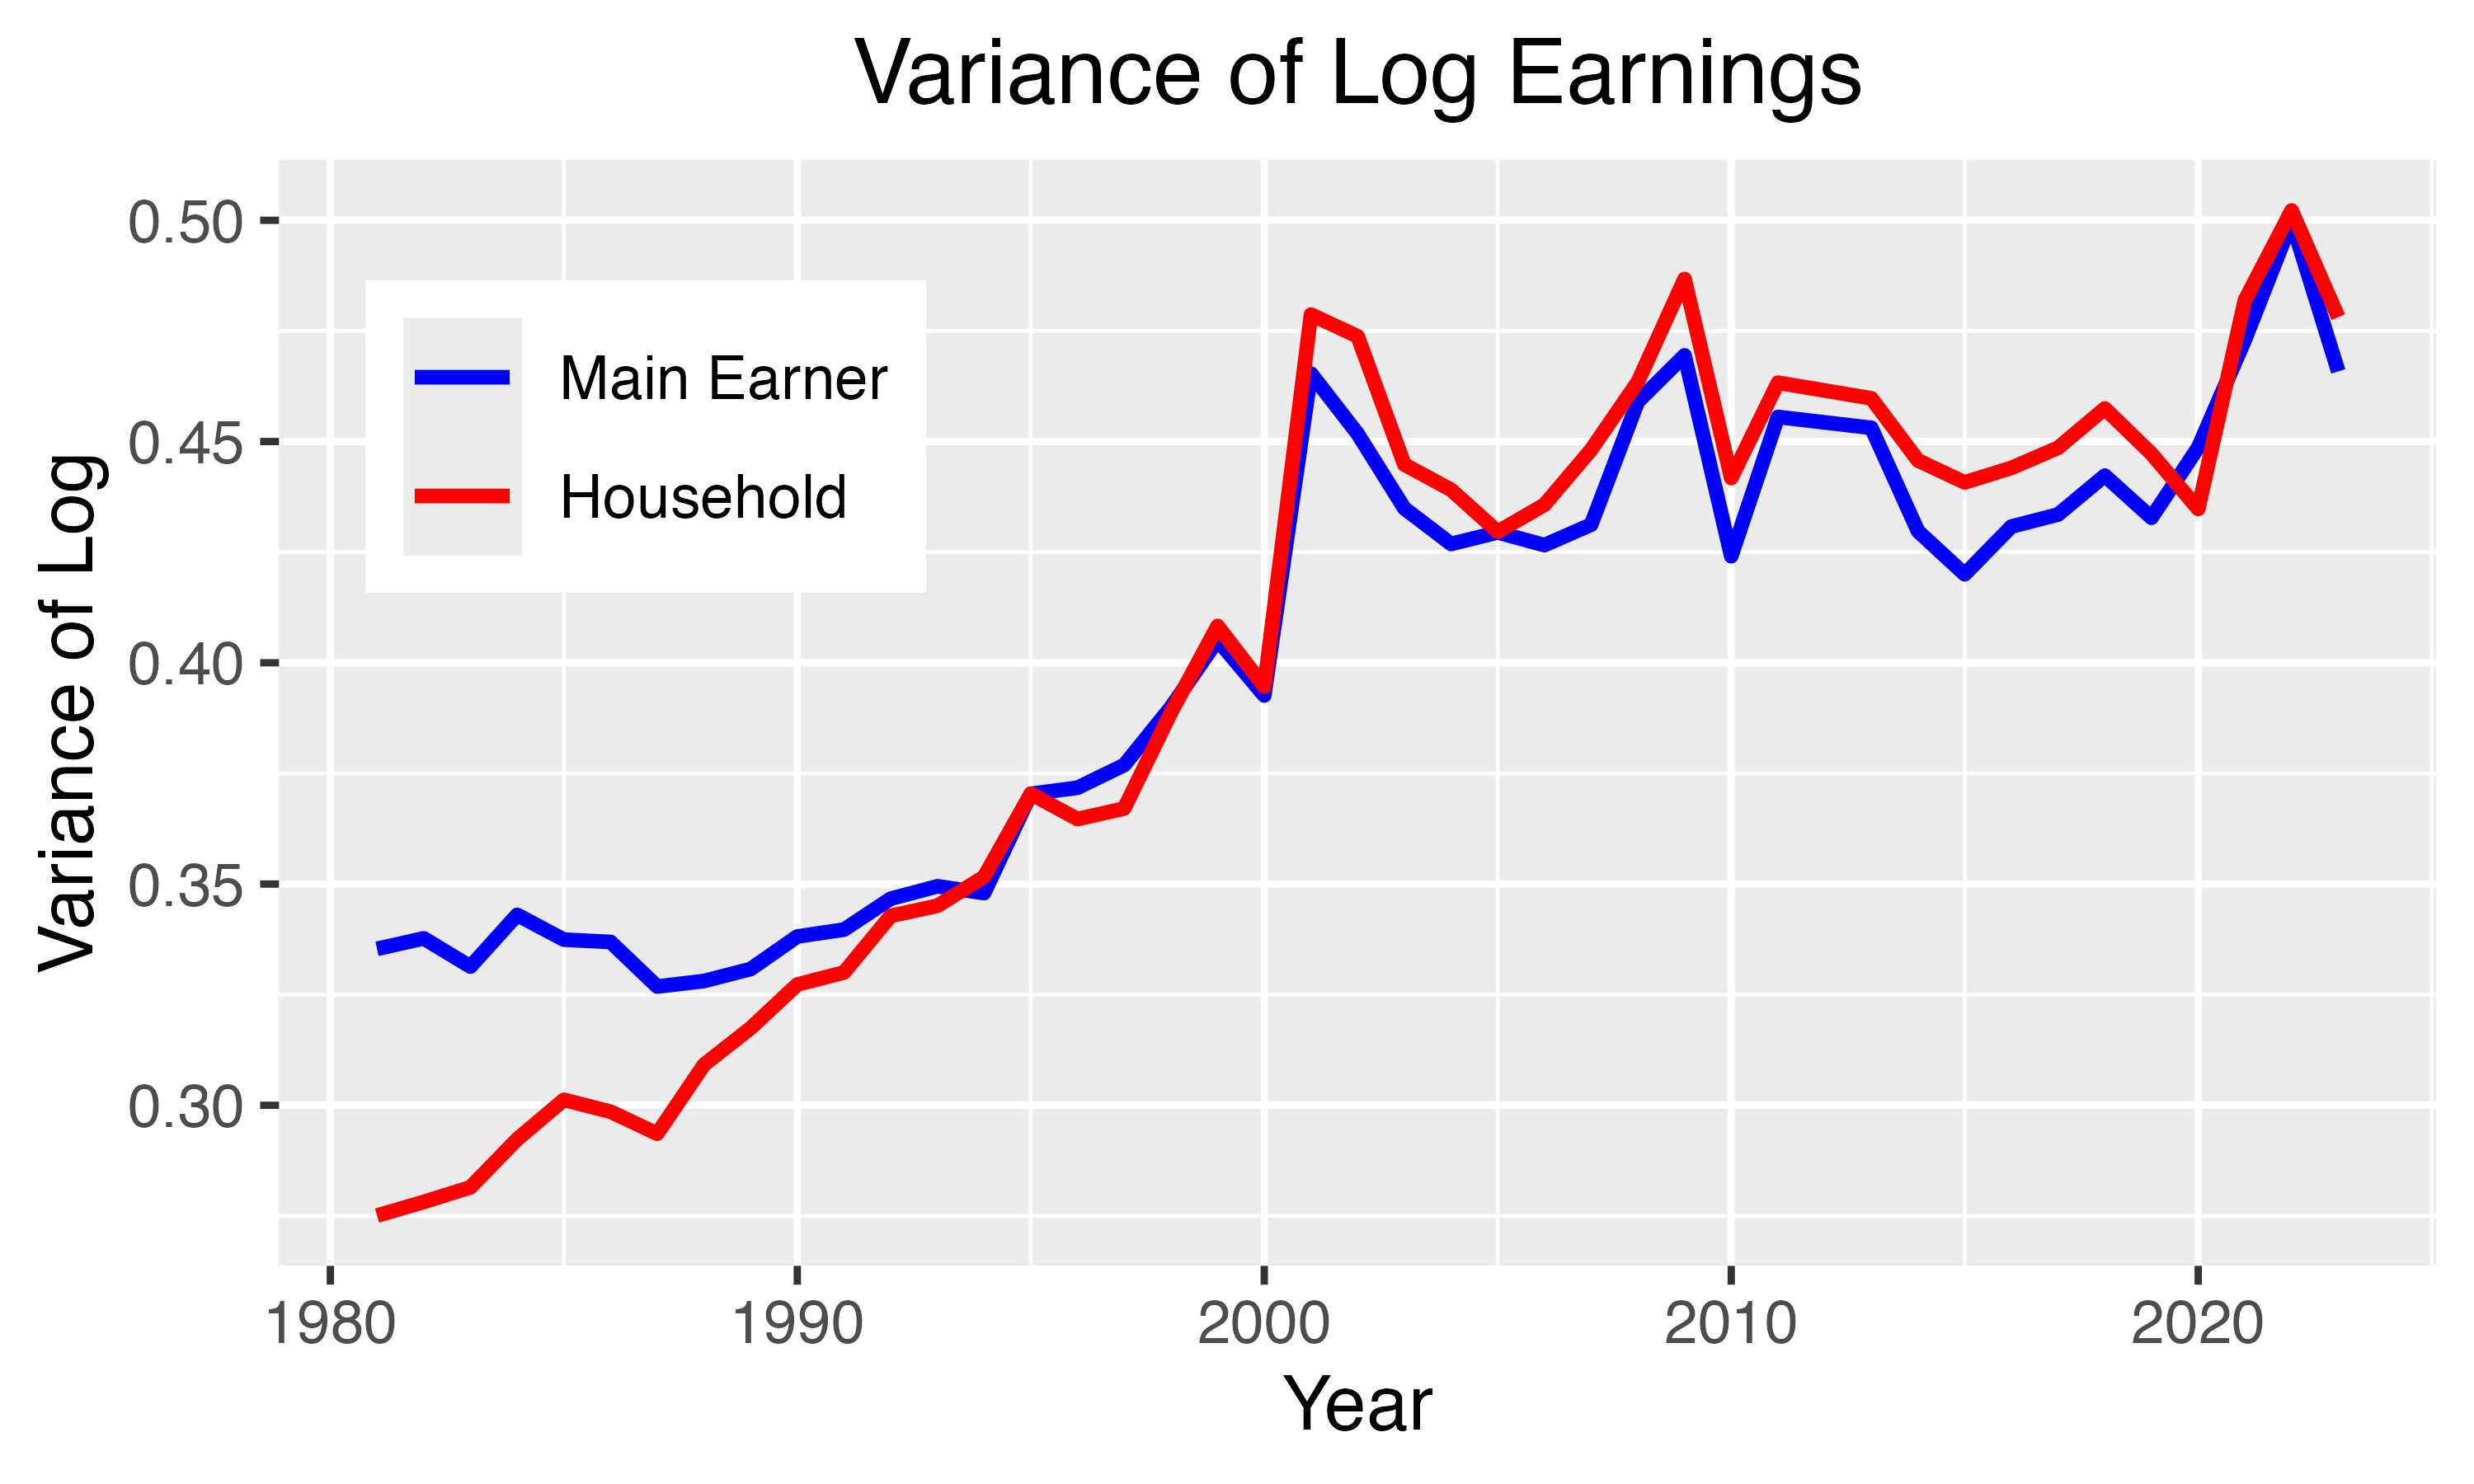
\includegraphics[width=\textwidth]{figures/Fig_3/Fig_3a_Var_indHH.png}
    \end{subfigure}
    \begin{subfigure}[t]{0.475\textwidth}
        \centering
        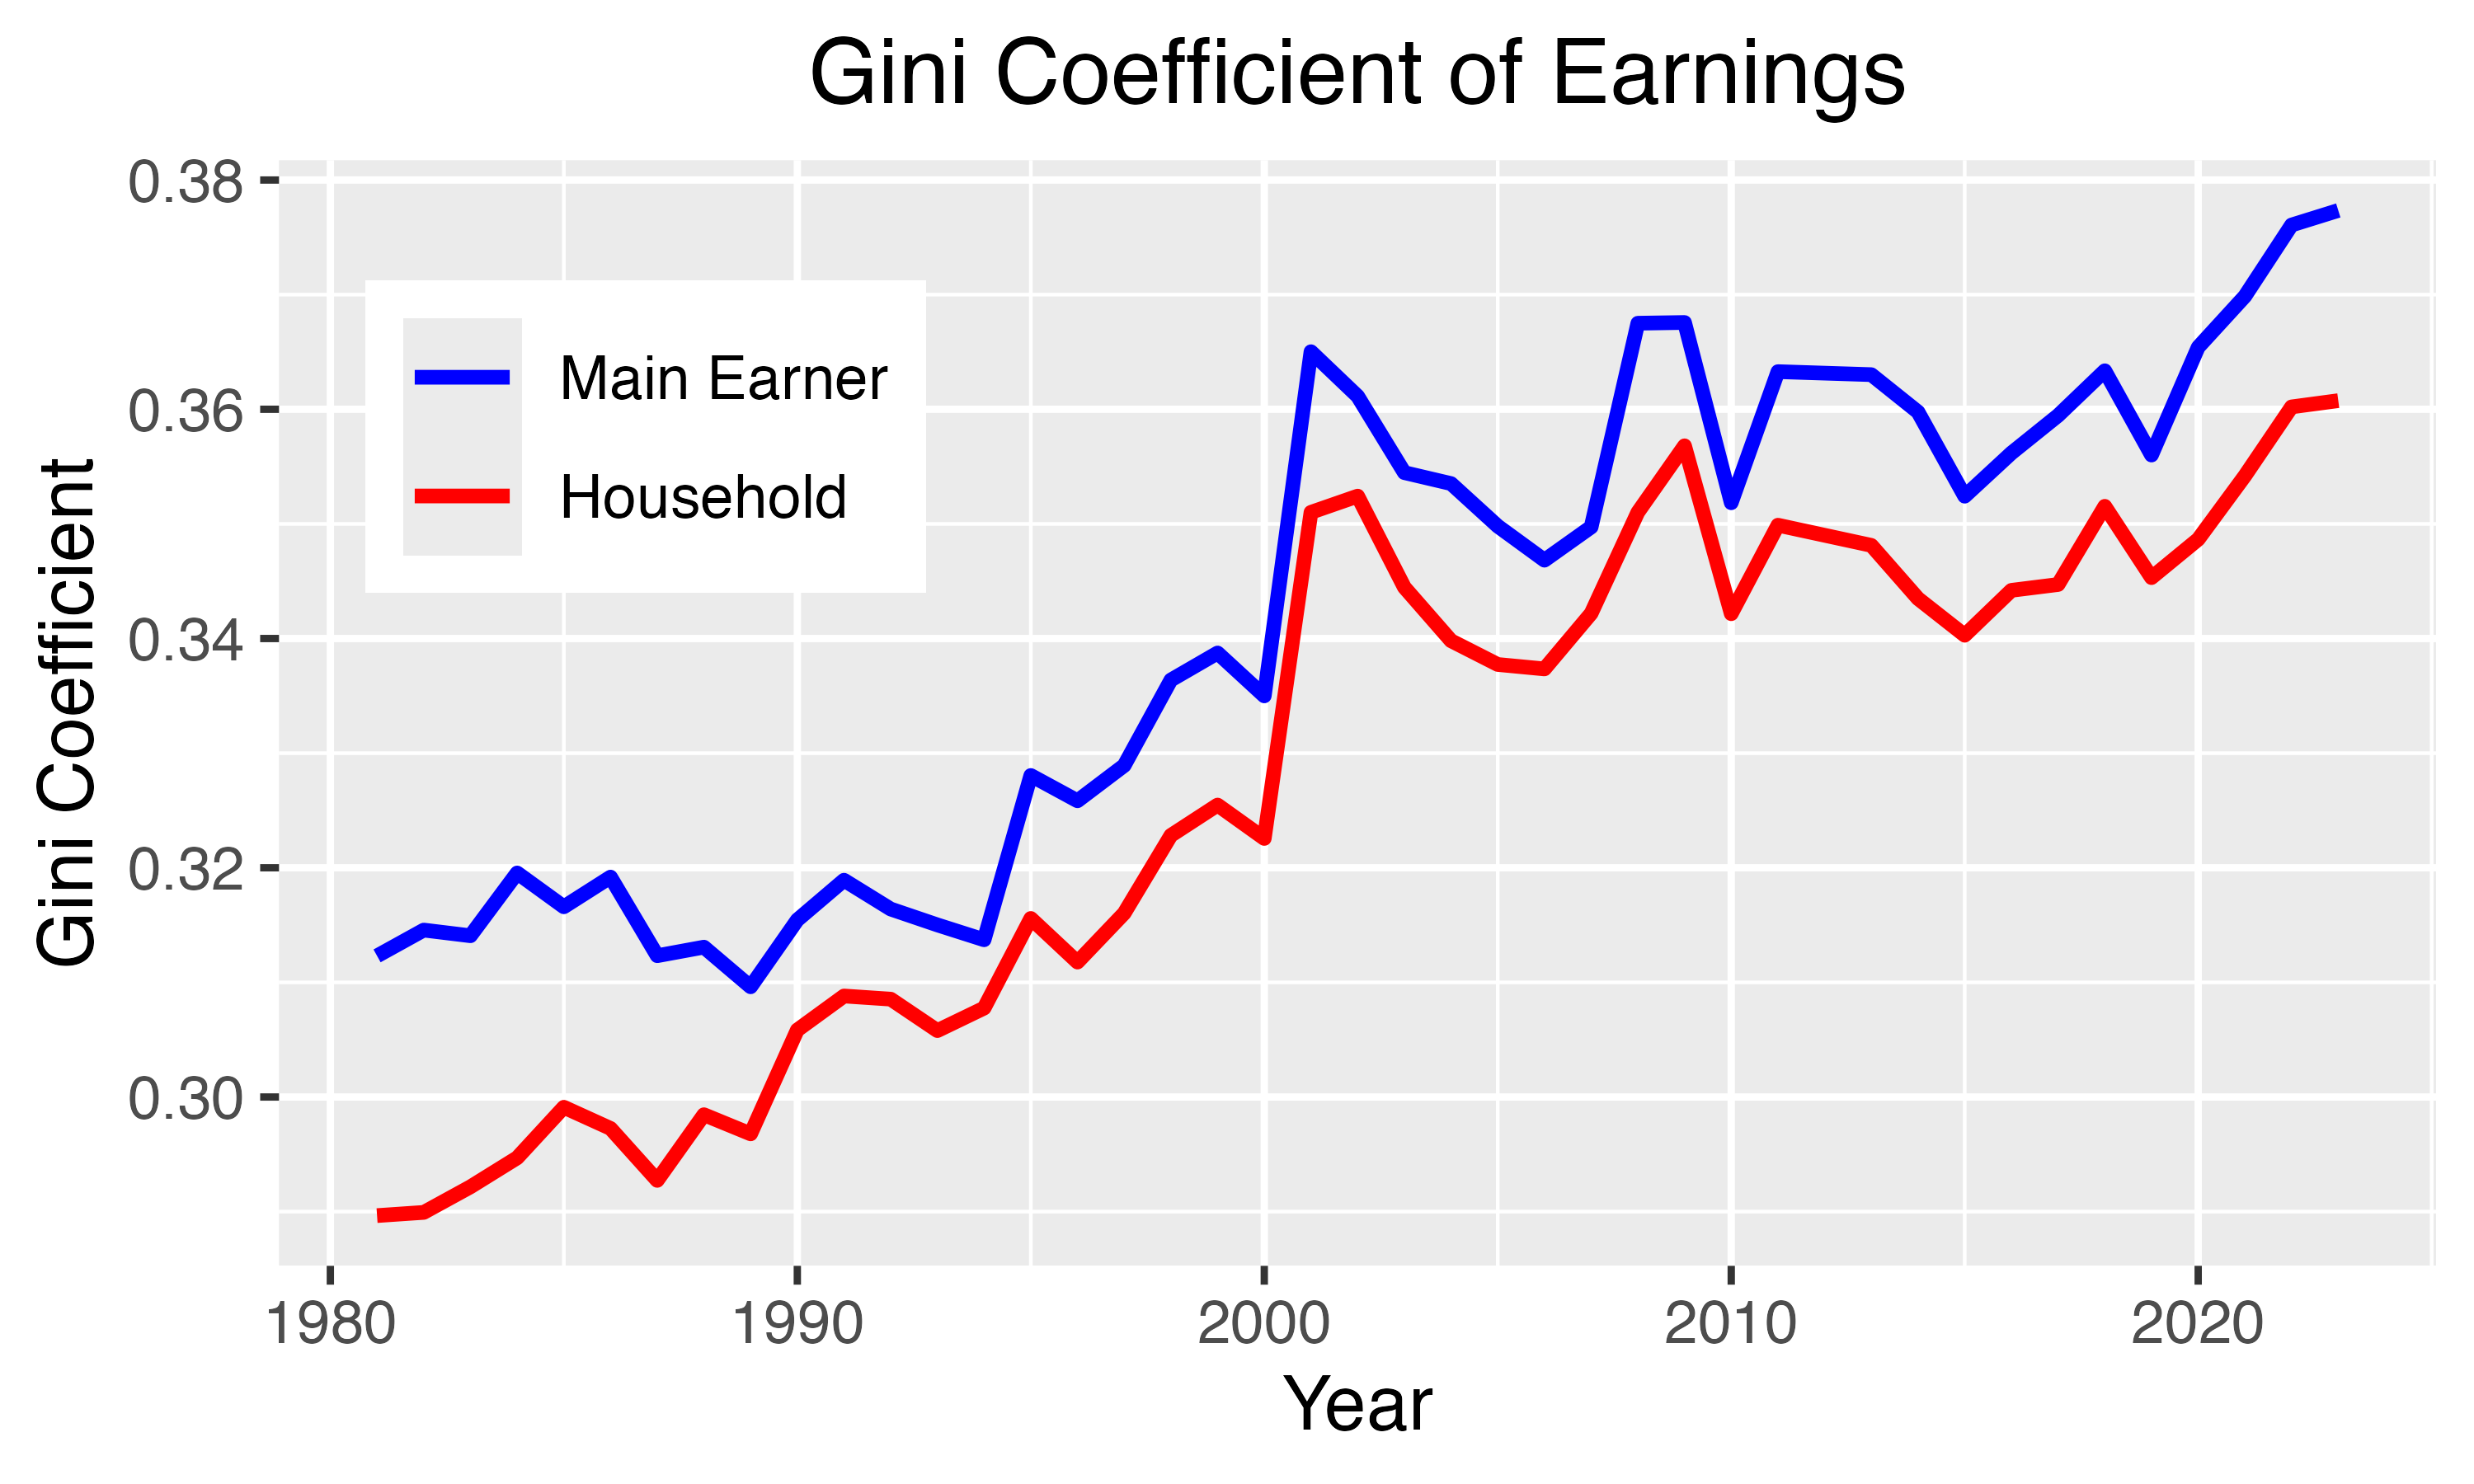
\includegraphics[width=\textwidth]{figures/Fig_3/Fig_3b_Gini_indHH.png}
    \end{subfigure}
    \begin{subfigure}[t]{0.475\textwidth}
        \centering
        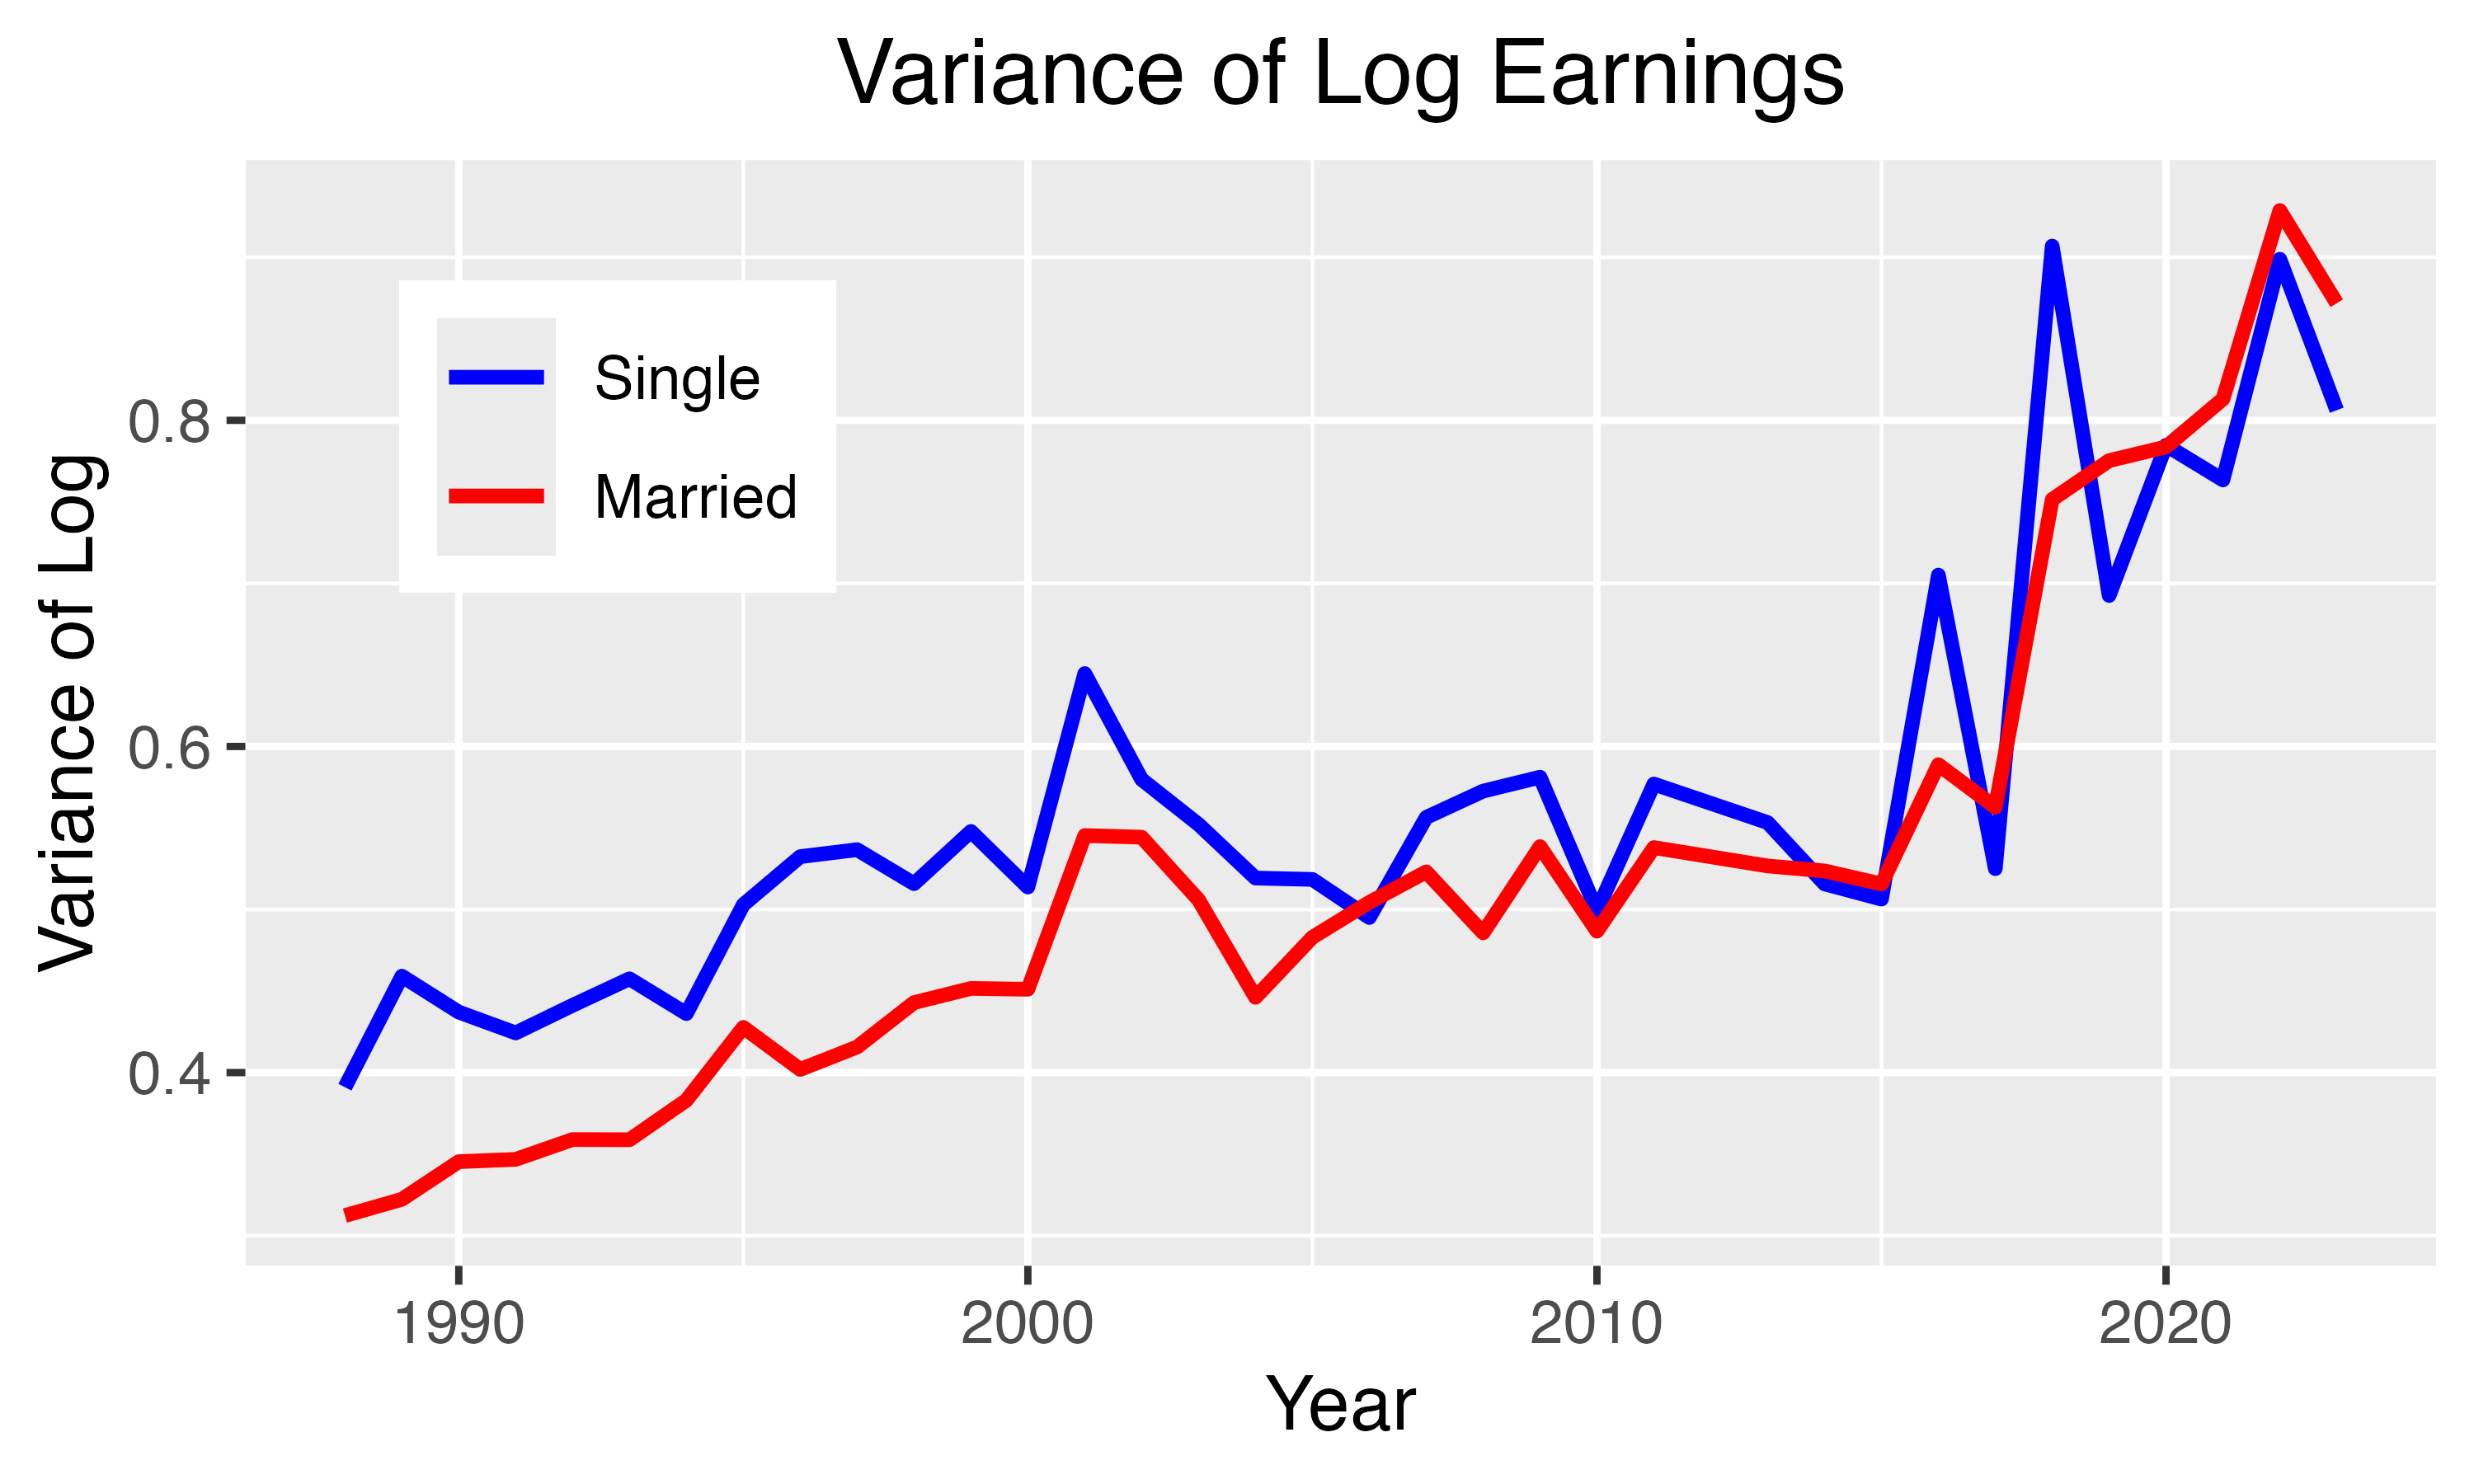
\includegraphics[width=\textwidth]{figures/Fig_3/Fig_3c_Var_single.png}
    \end{subfigure}
    \begin{subfigure}[t]{0.475\textwidth}
        \centering
        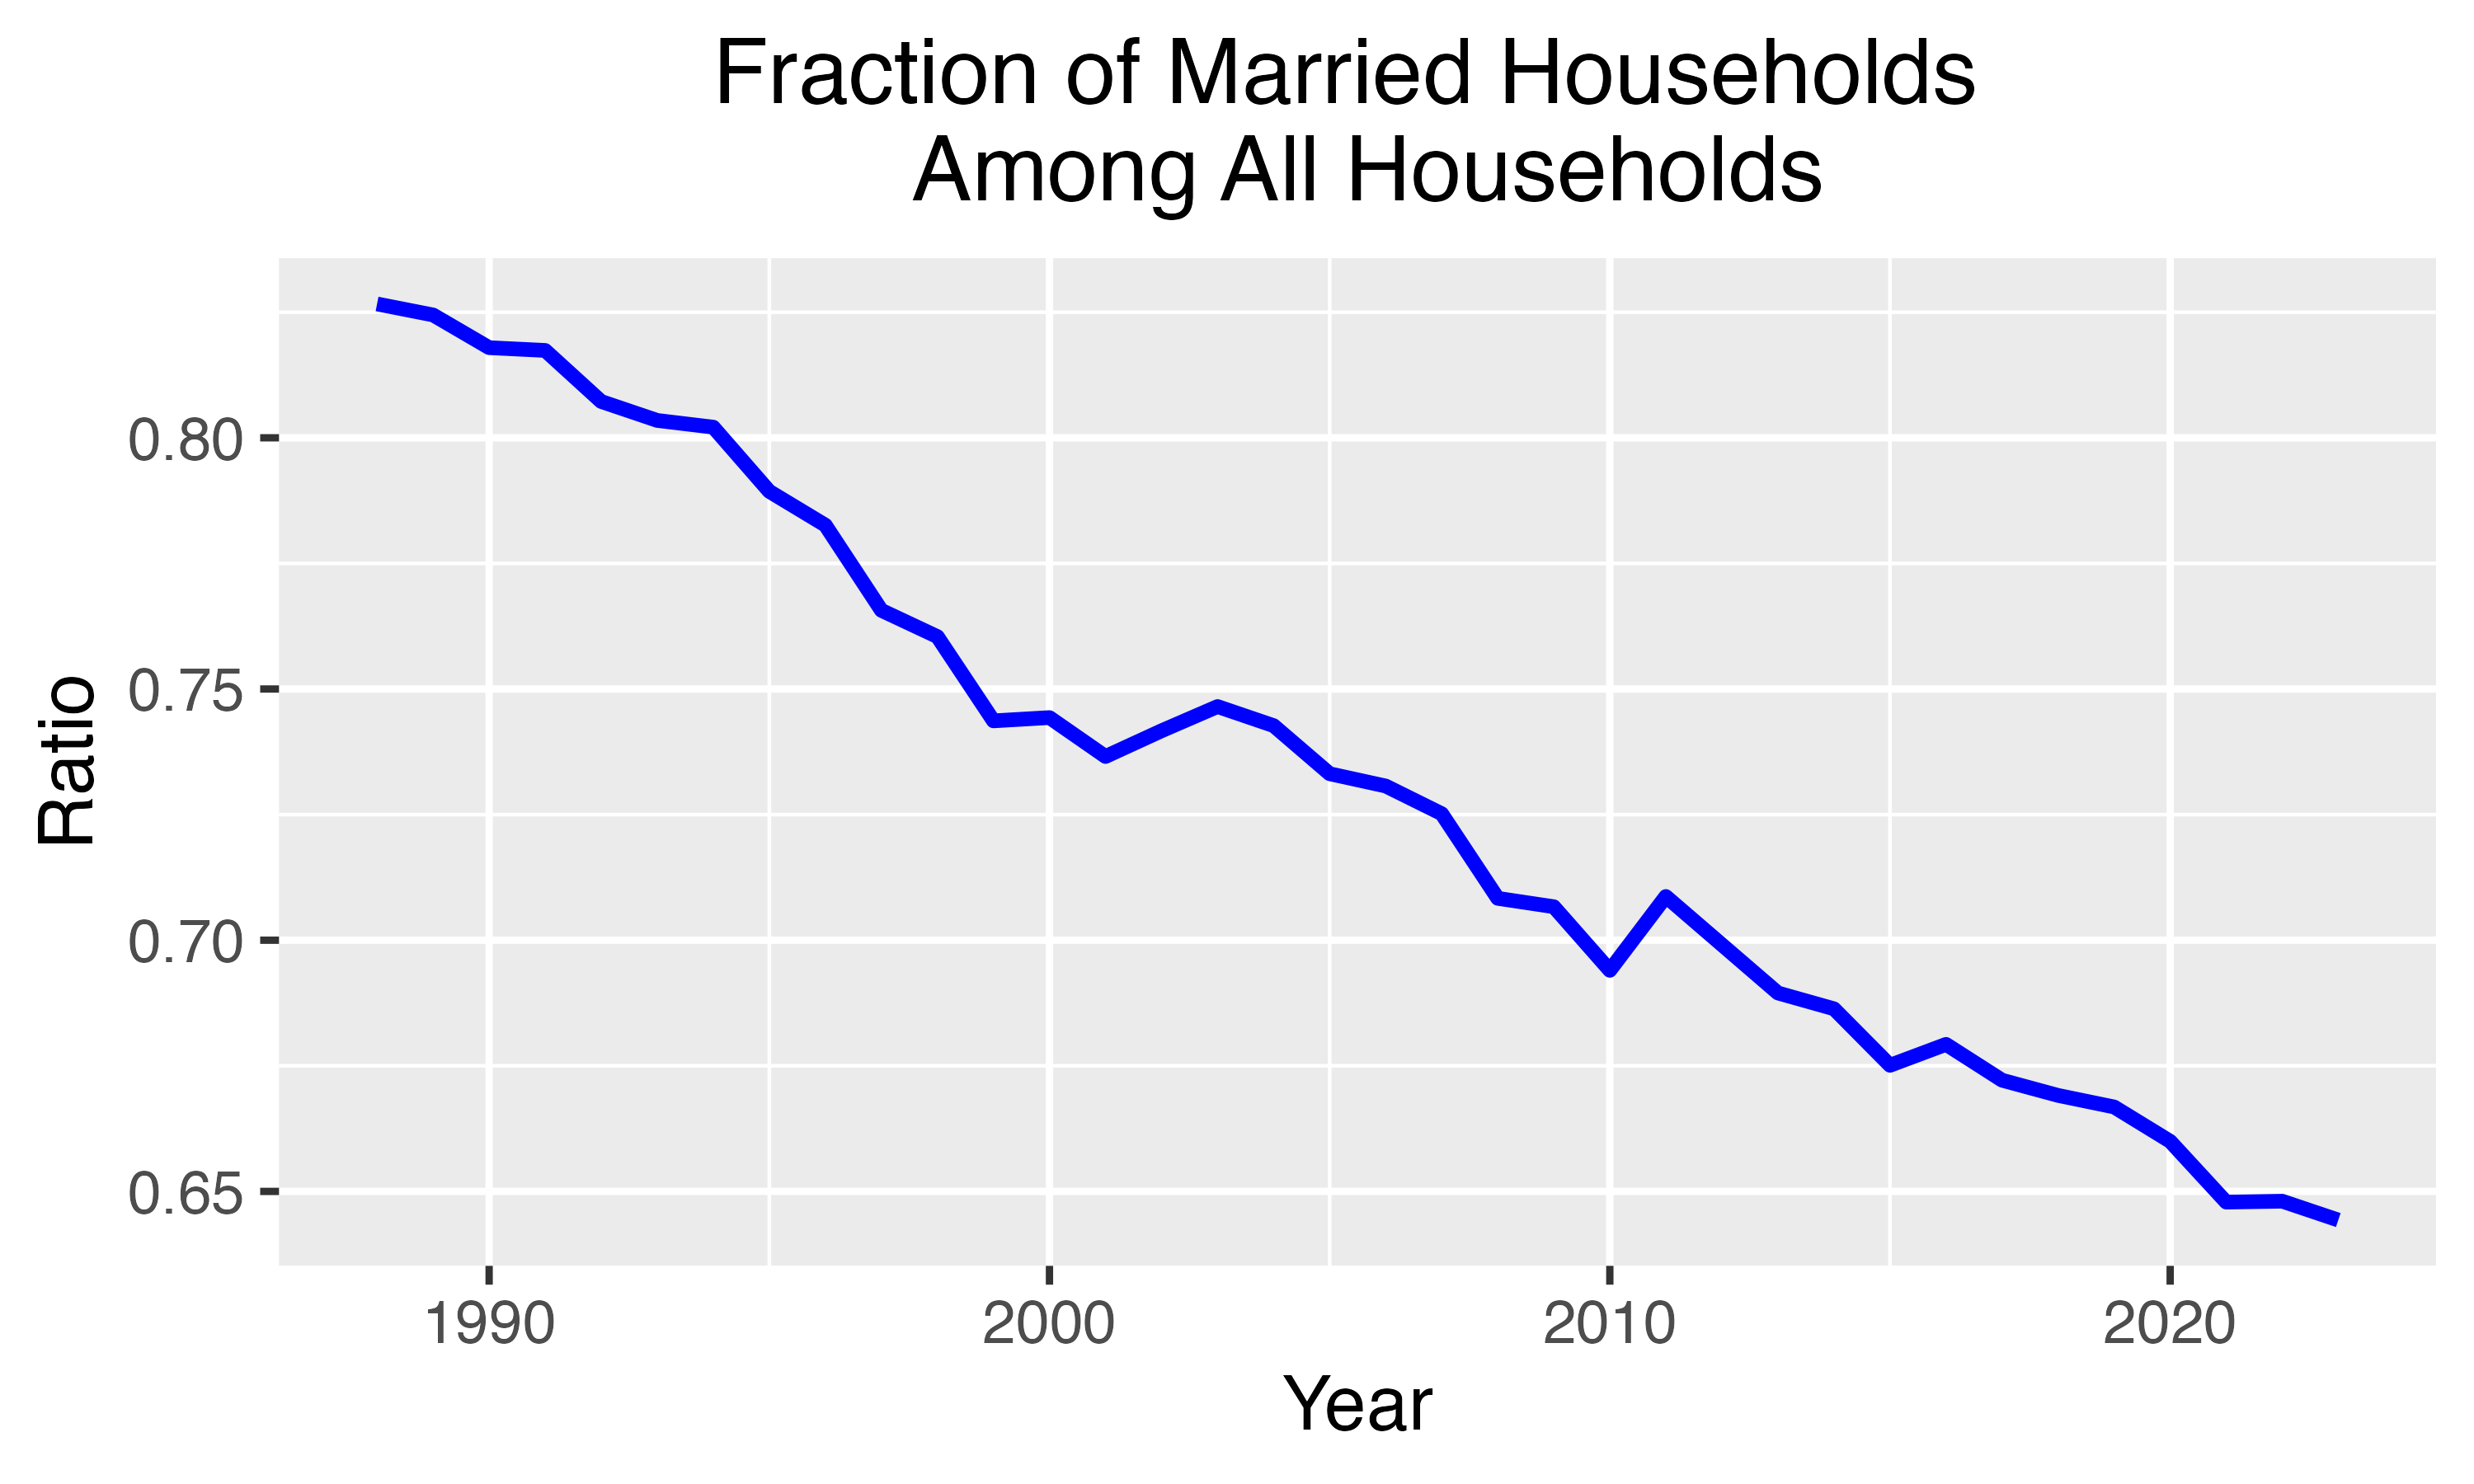
\includegraphics[width=\textwidth]{figures/Fig_3/Fig_3d_married_ratio.png}
    \end{subfigure}
    \begin{subfigure}[t]{0.475\textwidth}
        \centering
        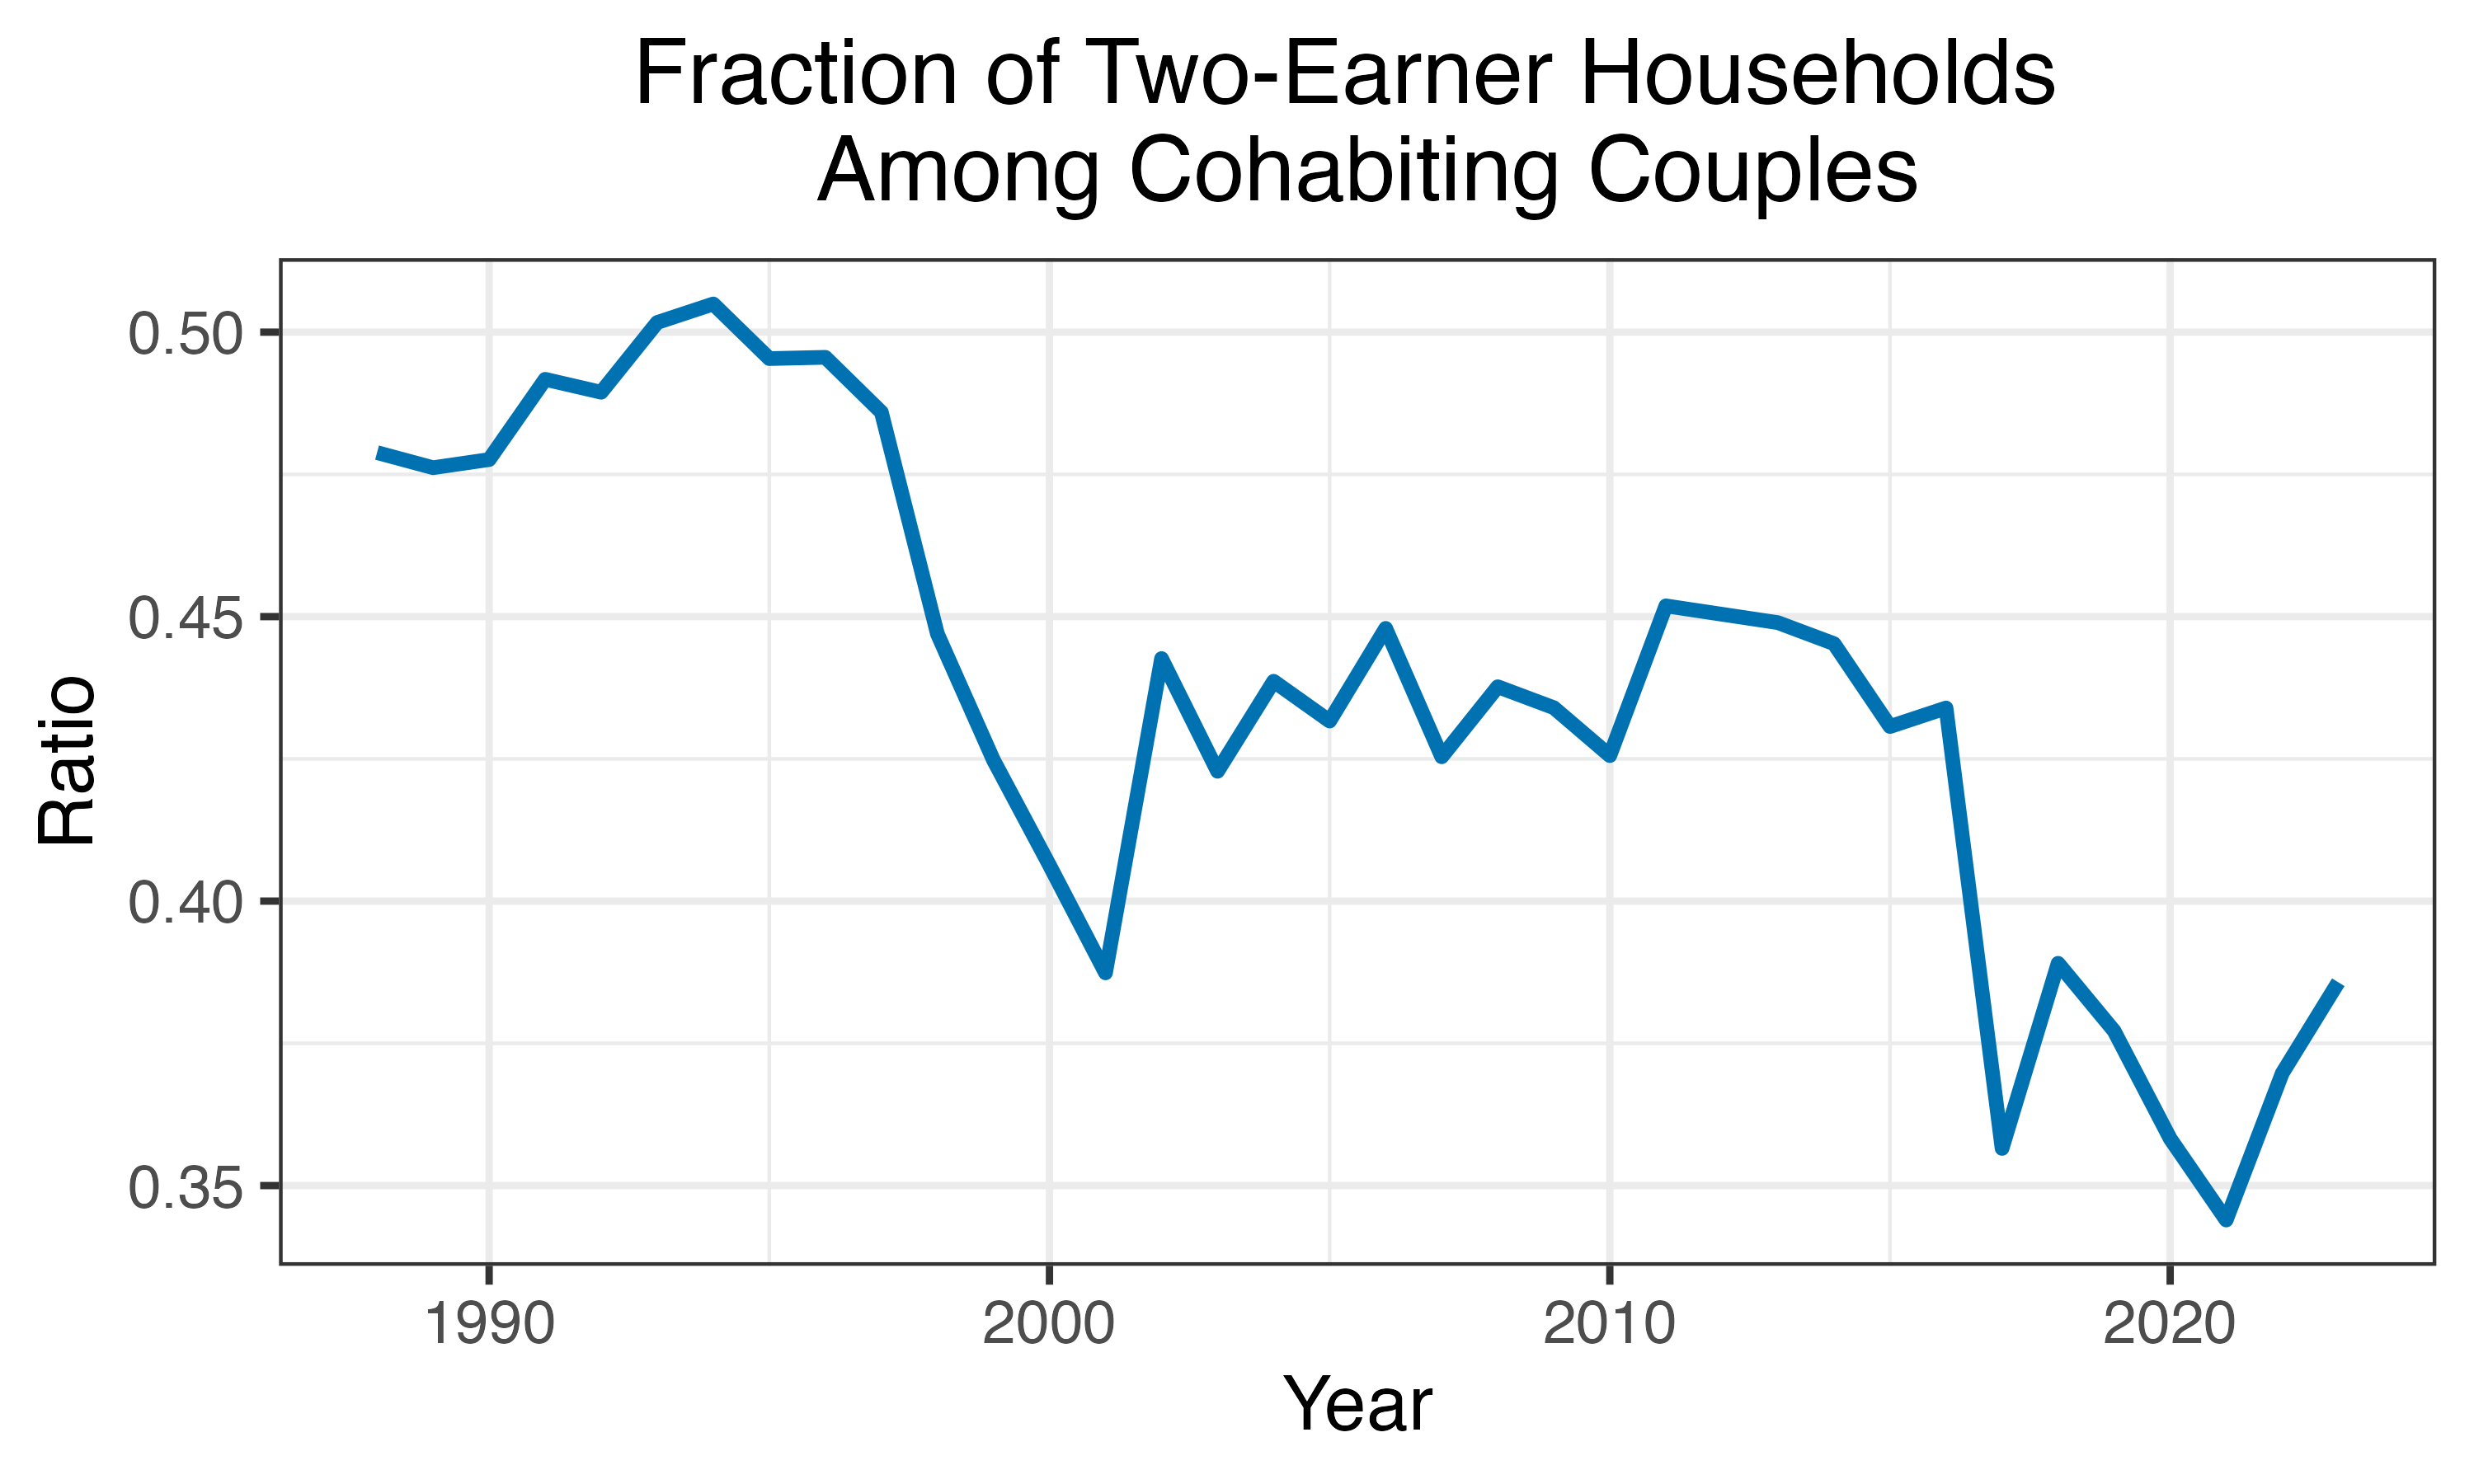
\includegraphics[width=\textwidth]{figures/Fig_3/Fig_3e_two_earner_ratio.png}
    \end{subfigure}
    \begin{subfigure}[t]{0.475\textwidth}
        \centering
        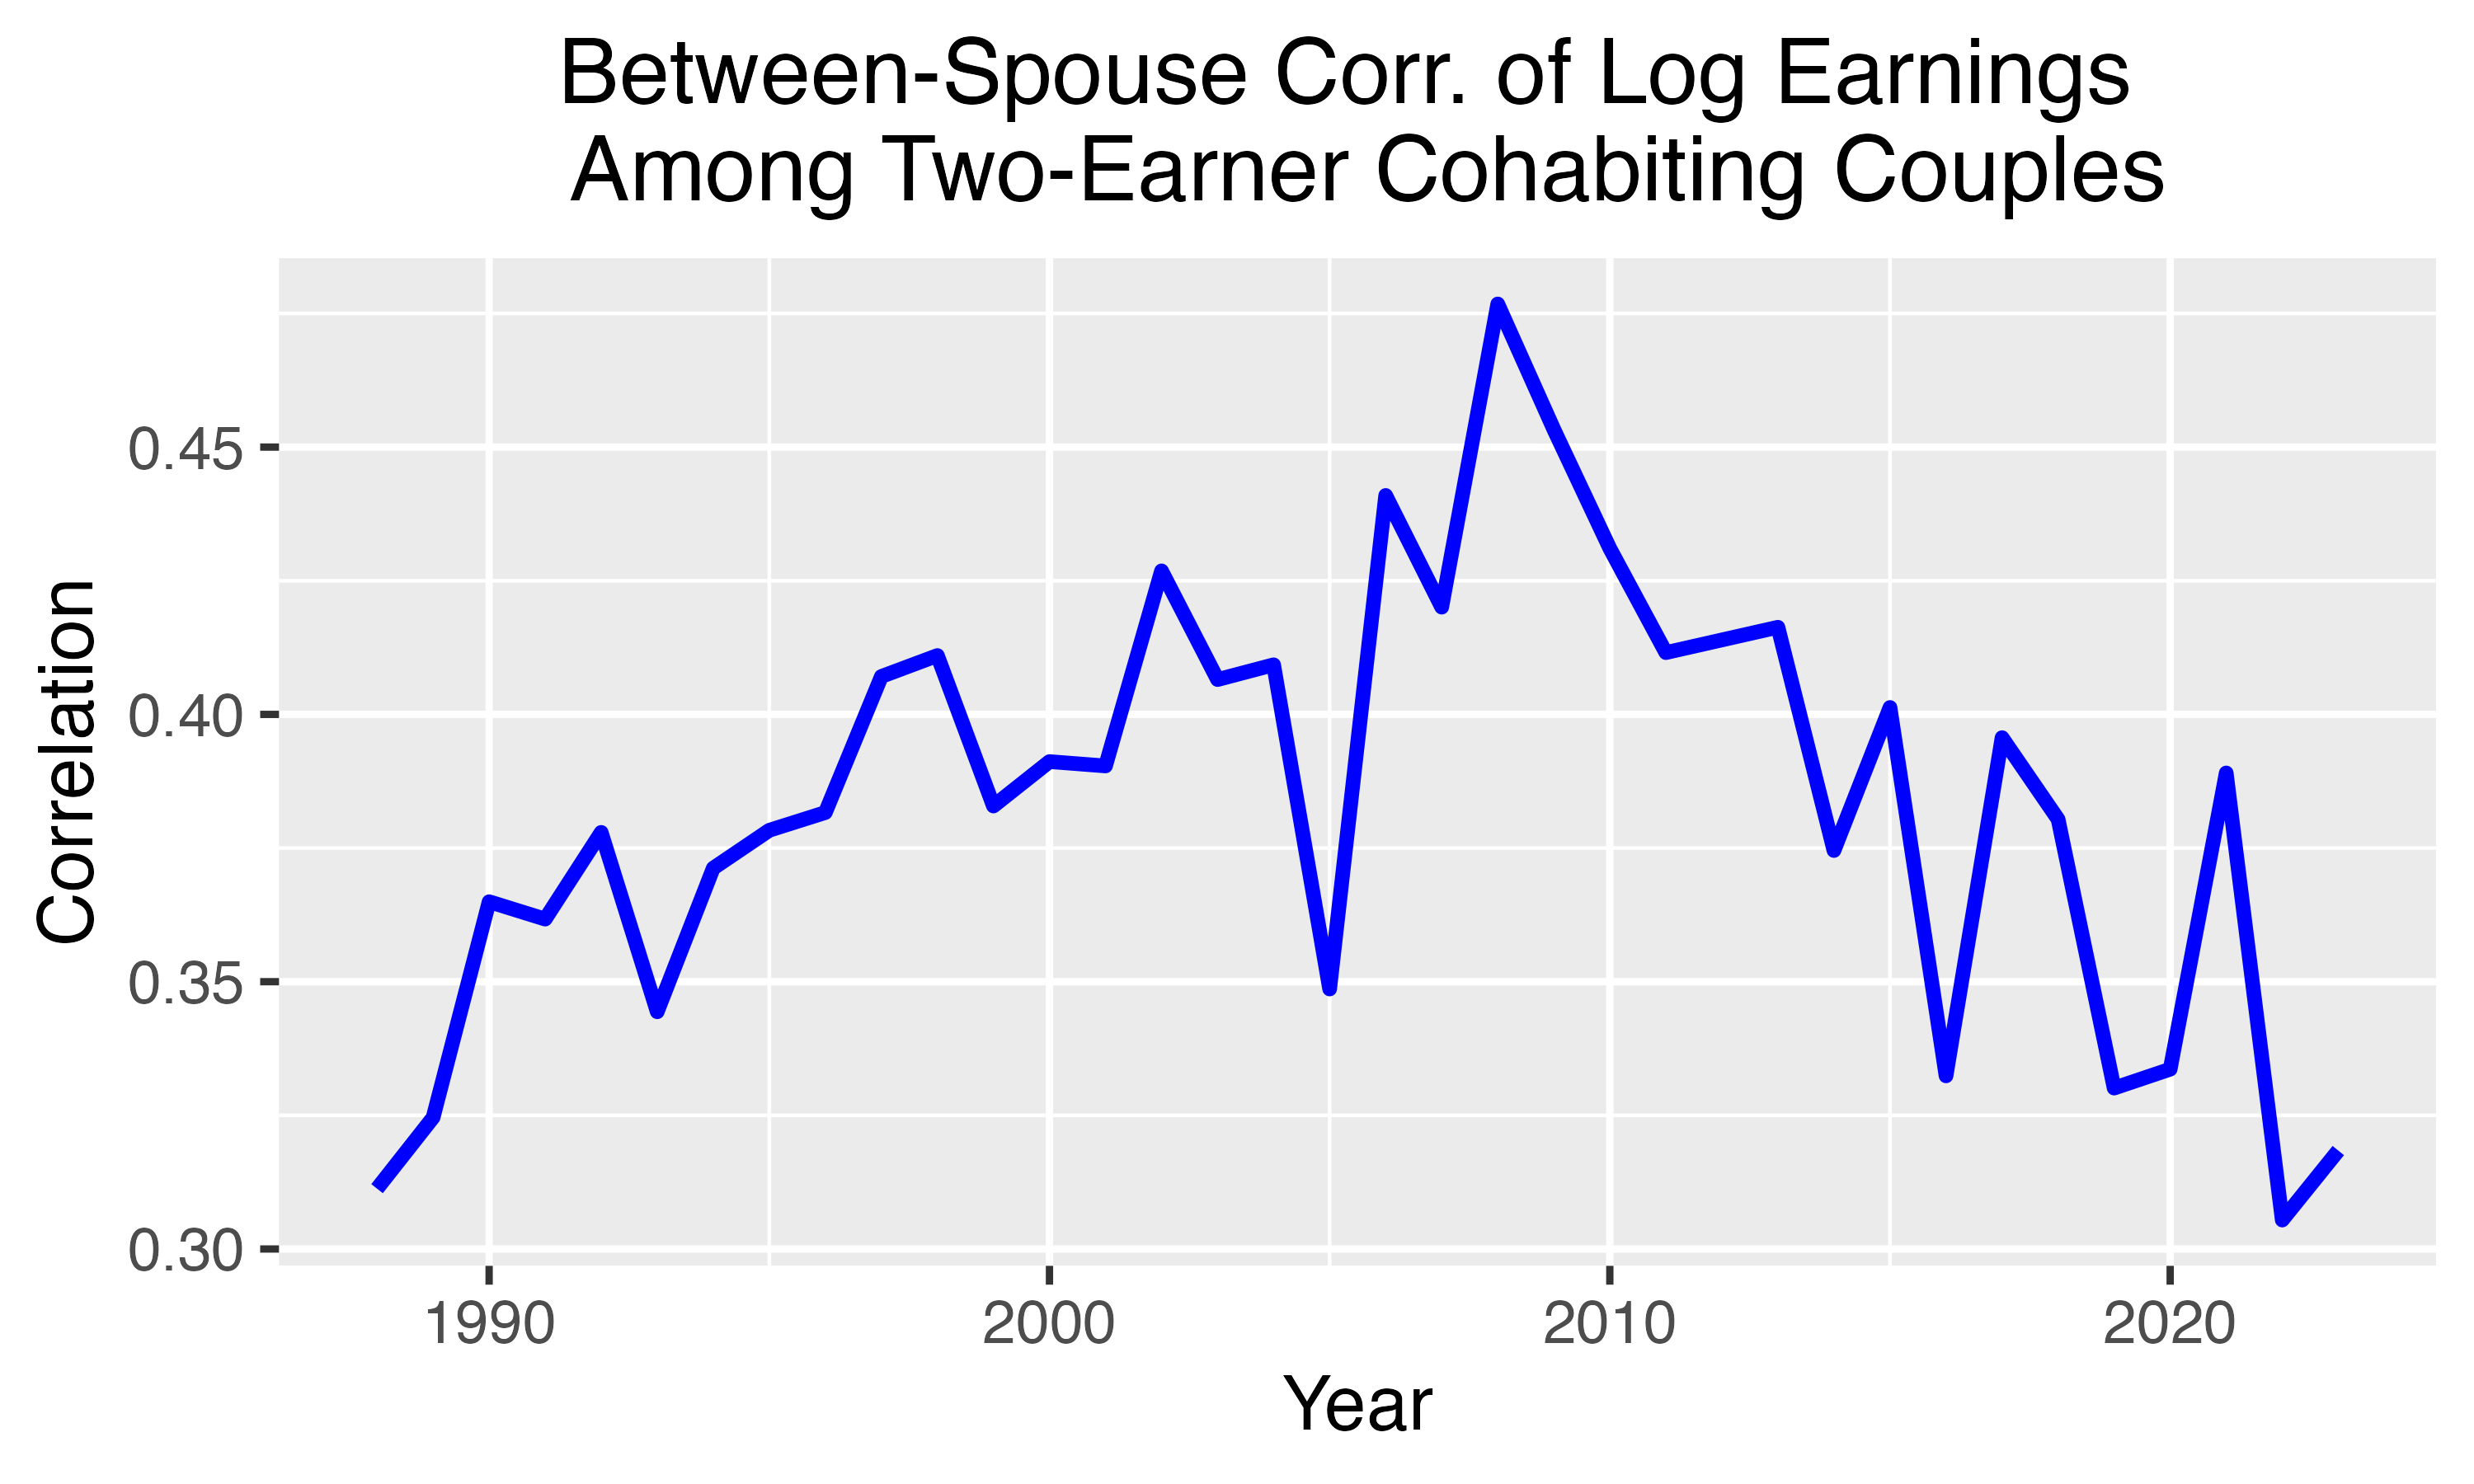
\includegraphics[width=\textwidth]{figures/Fig_3/Fig_3f_correlation.png}
    \end{subfigure}
    \caption{Understanding the role of the Family for Earnings Inequality}
    \label{fig:Indi_to_HH}
\end{figure}

Next, we look at the role of the family in household earnings inequality. The top two panels of Figure \ref{fig:Indi_to_HH} compare the main earner with the household. Both series are measured per adult equivalent, so the two share a common scale. 
The Gini coefficient behaves as income pooling predicts: household earnings are less unequal than the main earner's, indicating that resources are shared within the family. 
The variance of log earnings tells a weaker story. Household variance lies below the main earner's until 1993. From 1994, however, the two overlap, with the household above in 25 of the 29 years. Heathcote, Perri, and Violante (\citeyear{HEATHCOTE_2010}) find the same pattern for the US, where the two variances are strikingly similar while the two Gini coefficients differ. 
They attribute this to households at the bottom of the earnings distribution being either single or married with only one earner, so that pooling does little in the lower tail, which is where the variance of logs puts most of its weight. The same explanation is plausible for Taiwan, given the falling shares of married and two-earner households in the panels below. 

Appendix Figure \ref{fig:appendix_indHH_raw} repeats the comparison with the main earner left on a per-earner scale, as an unequivalized individual series would be plotted. On that scale the household lies above the main earner in 41 of 42 years for the variance and in every year for the Gini, so the ordering is sensitive to the choice of scale. 

Turning to household structure, the bottom left panel of Figure \ref{fig:Indi_to_HH} shows that the share of two-earner households has been decreasing in our dataset, which is not usually the case. The decline we observe could be due to higher-income couples splitting their household registration, which can reduce housing and land taxes. The middle two panels of Figure \ref{fig:Indi_to_HH} show the relation between single and married households. Earnings are more dispersed among single households than among married ones in most years, as pooling within couples would predict. But the gap narrows from 0.06 in 1988 to below 0.03 from 2013 onward, and reverses in 2020 and 2023. The narrowing coincides with the decreasing fraction of married households. 

The bottom right panel shows the between-spouse earnings correlation among two-earner cohabiting households. Increasing assortative matching would lead one to expect this correlation to rise over time, as couples increasingly share educational background and earnings potential. It does rise, from 0.34 in 1988 to 0.49 in 2009, but then falls back, ending at 0.39 in 2023. 
One possible explanation for the reversal is the change in household structure discussed above. If higher-income couples separate their household registration, they leave the two-earner sample and drop out of this calculation entirely. Testing that would require linkage across years, which the SFIE does not provide, so the question is left open.

\subsection{Private Transfers and Asset Income}

\begin{figure}
    \centering
    \begin{subfigure}[t]{0.475\textwidth}
        \centering
        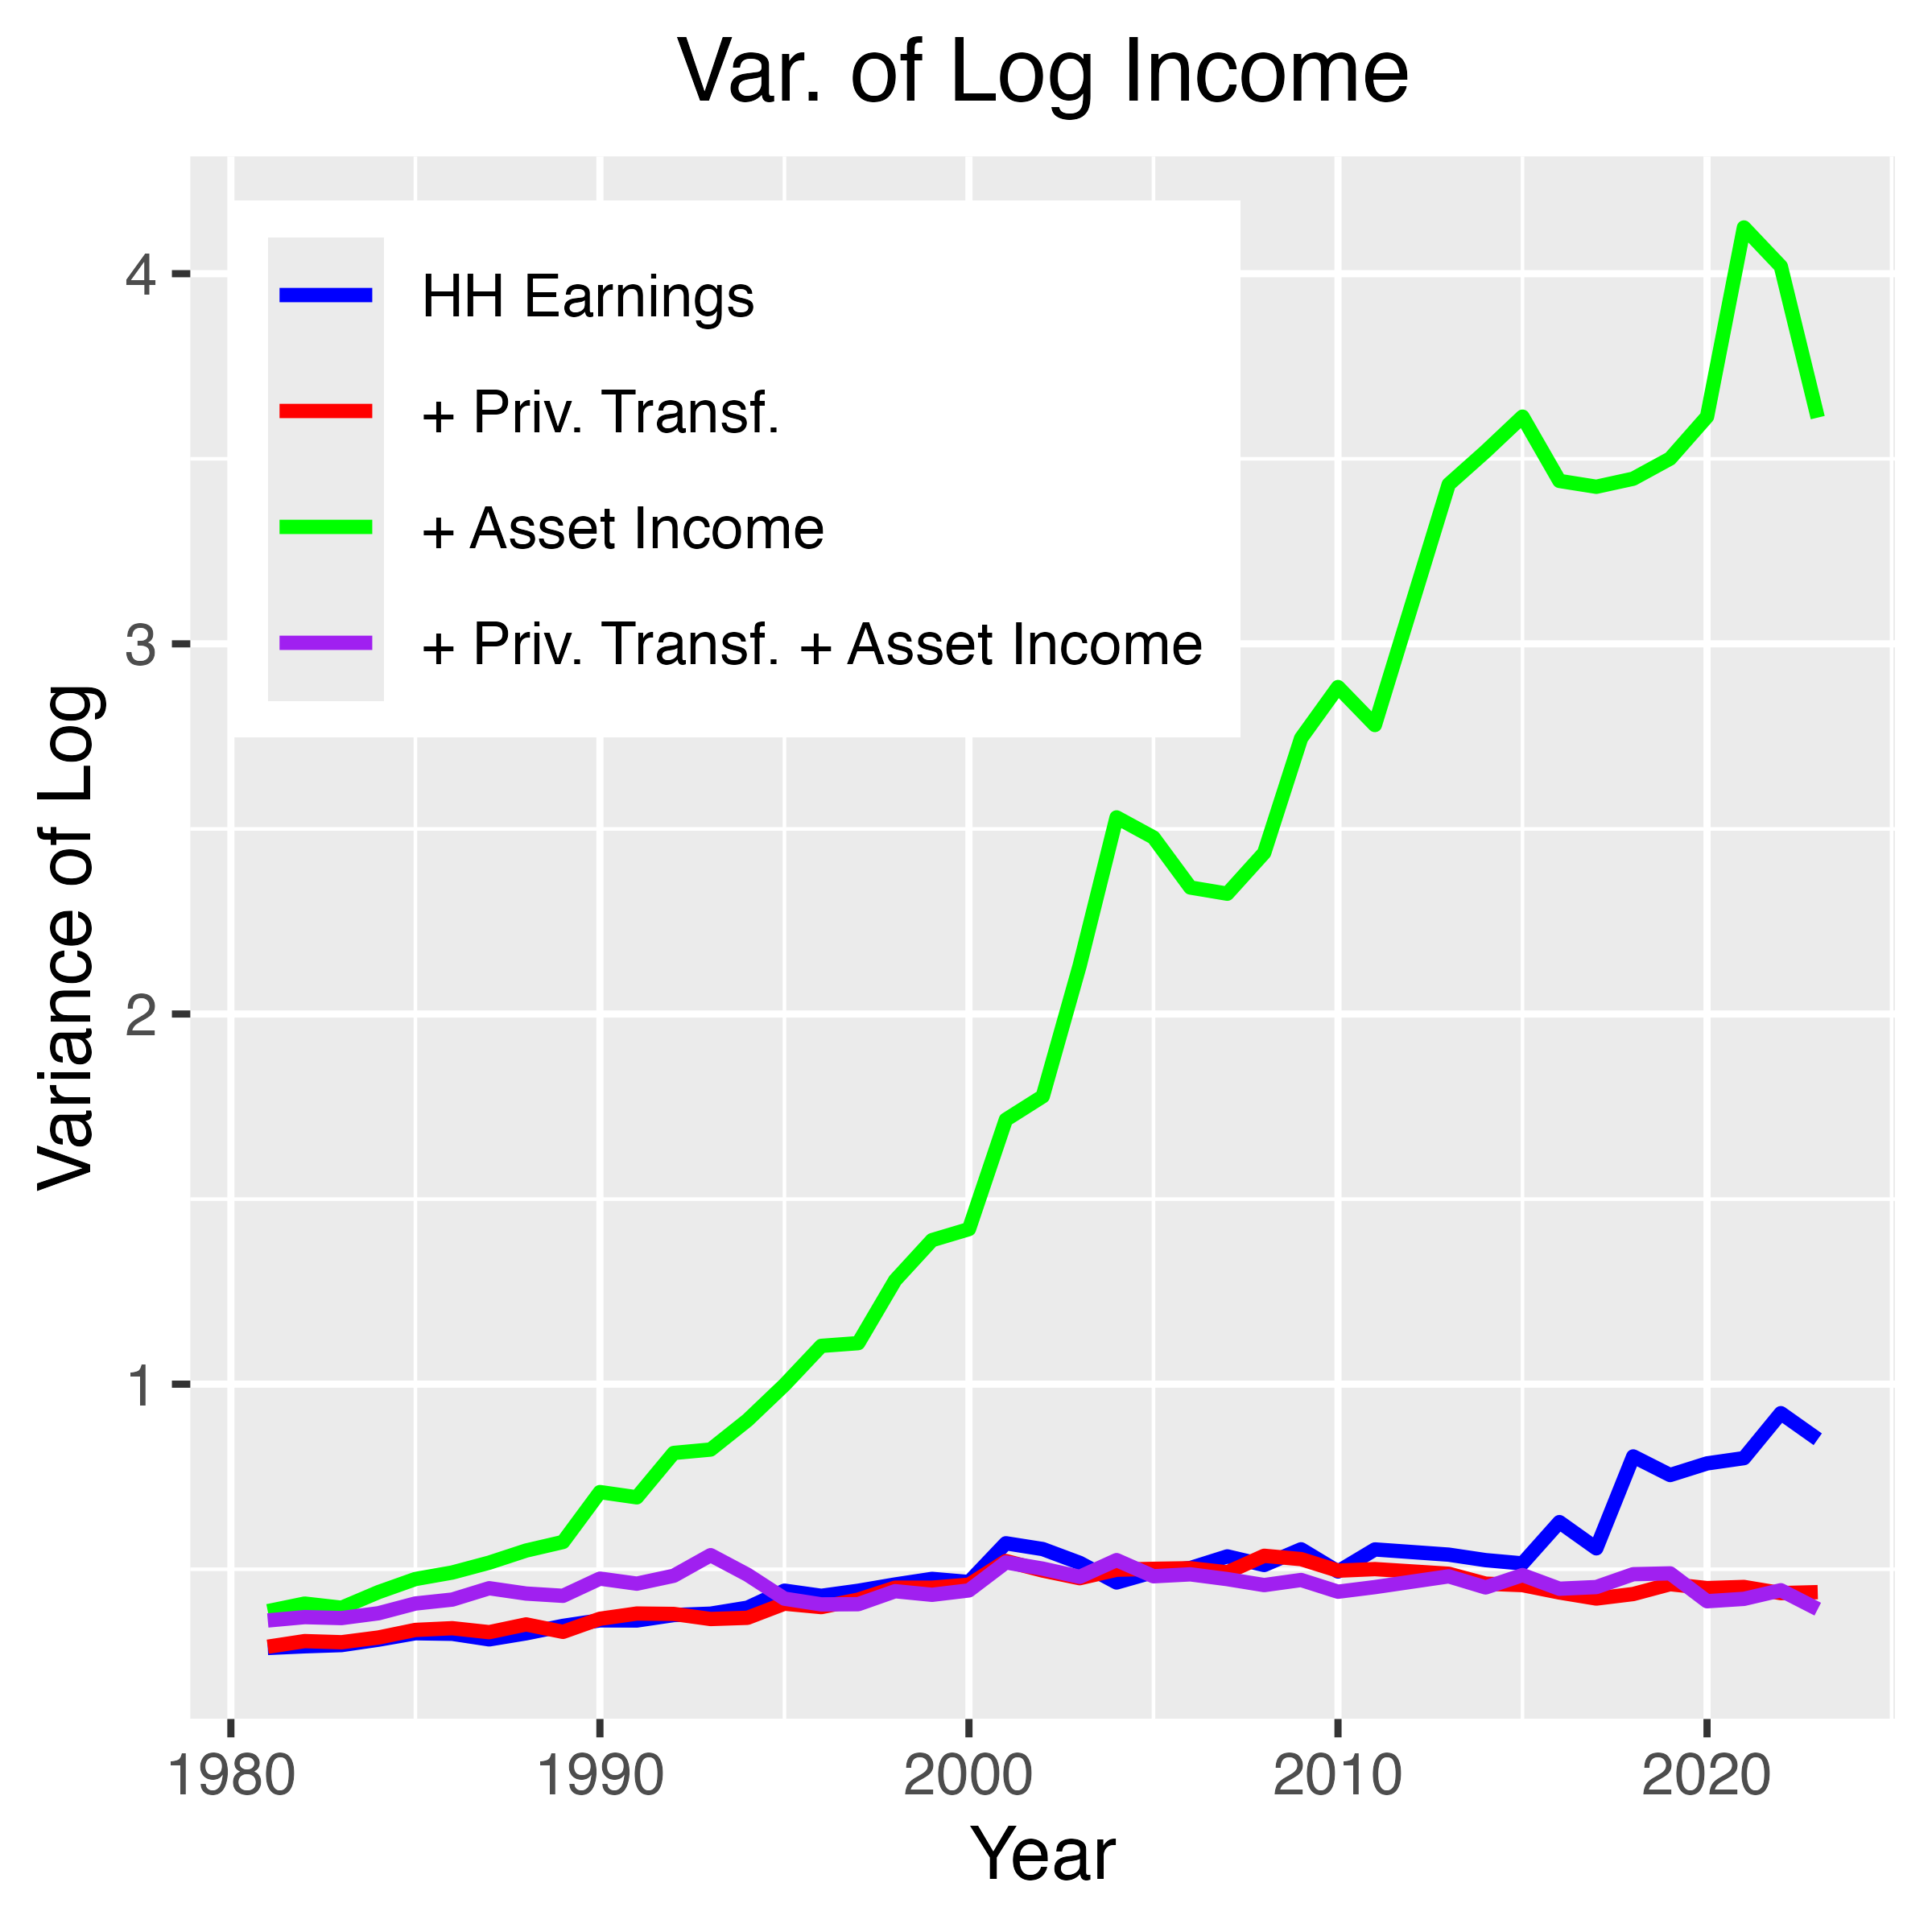
\includegraphics[width=\textwidth]{figures/Fig_4/Fig_4a_Var_inc.png}
    \end{subfigure}
    \begin{subfigure}[t]{0.475\textwidth}
        \centering
        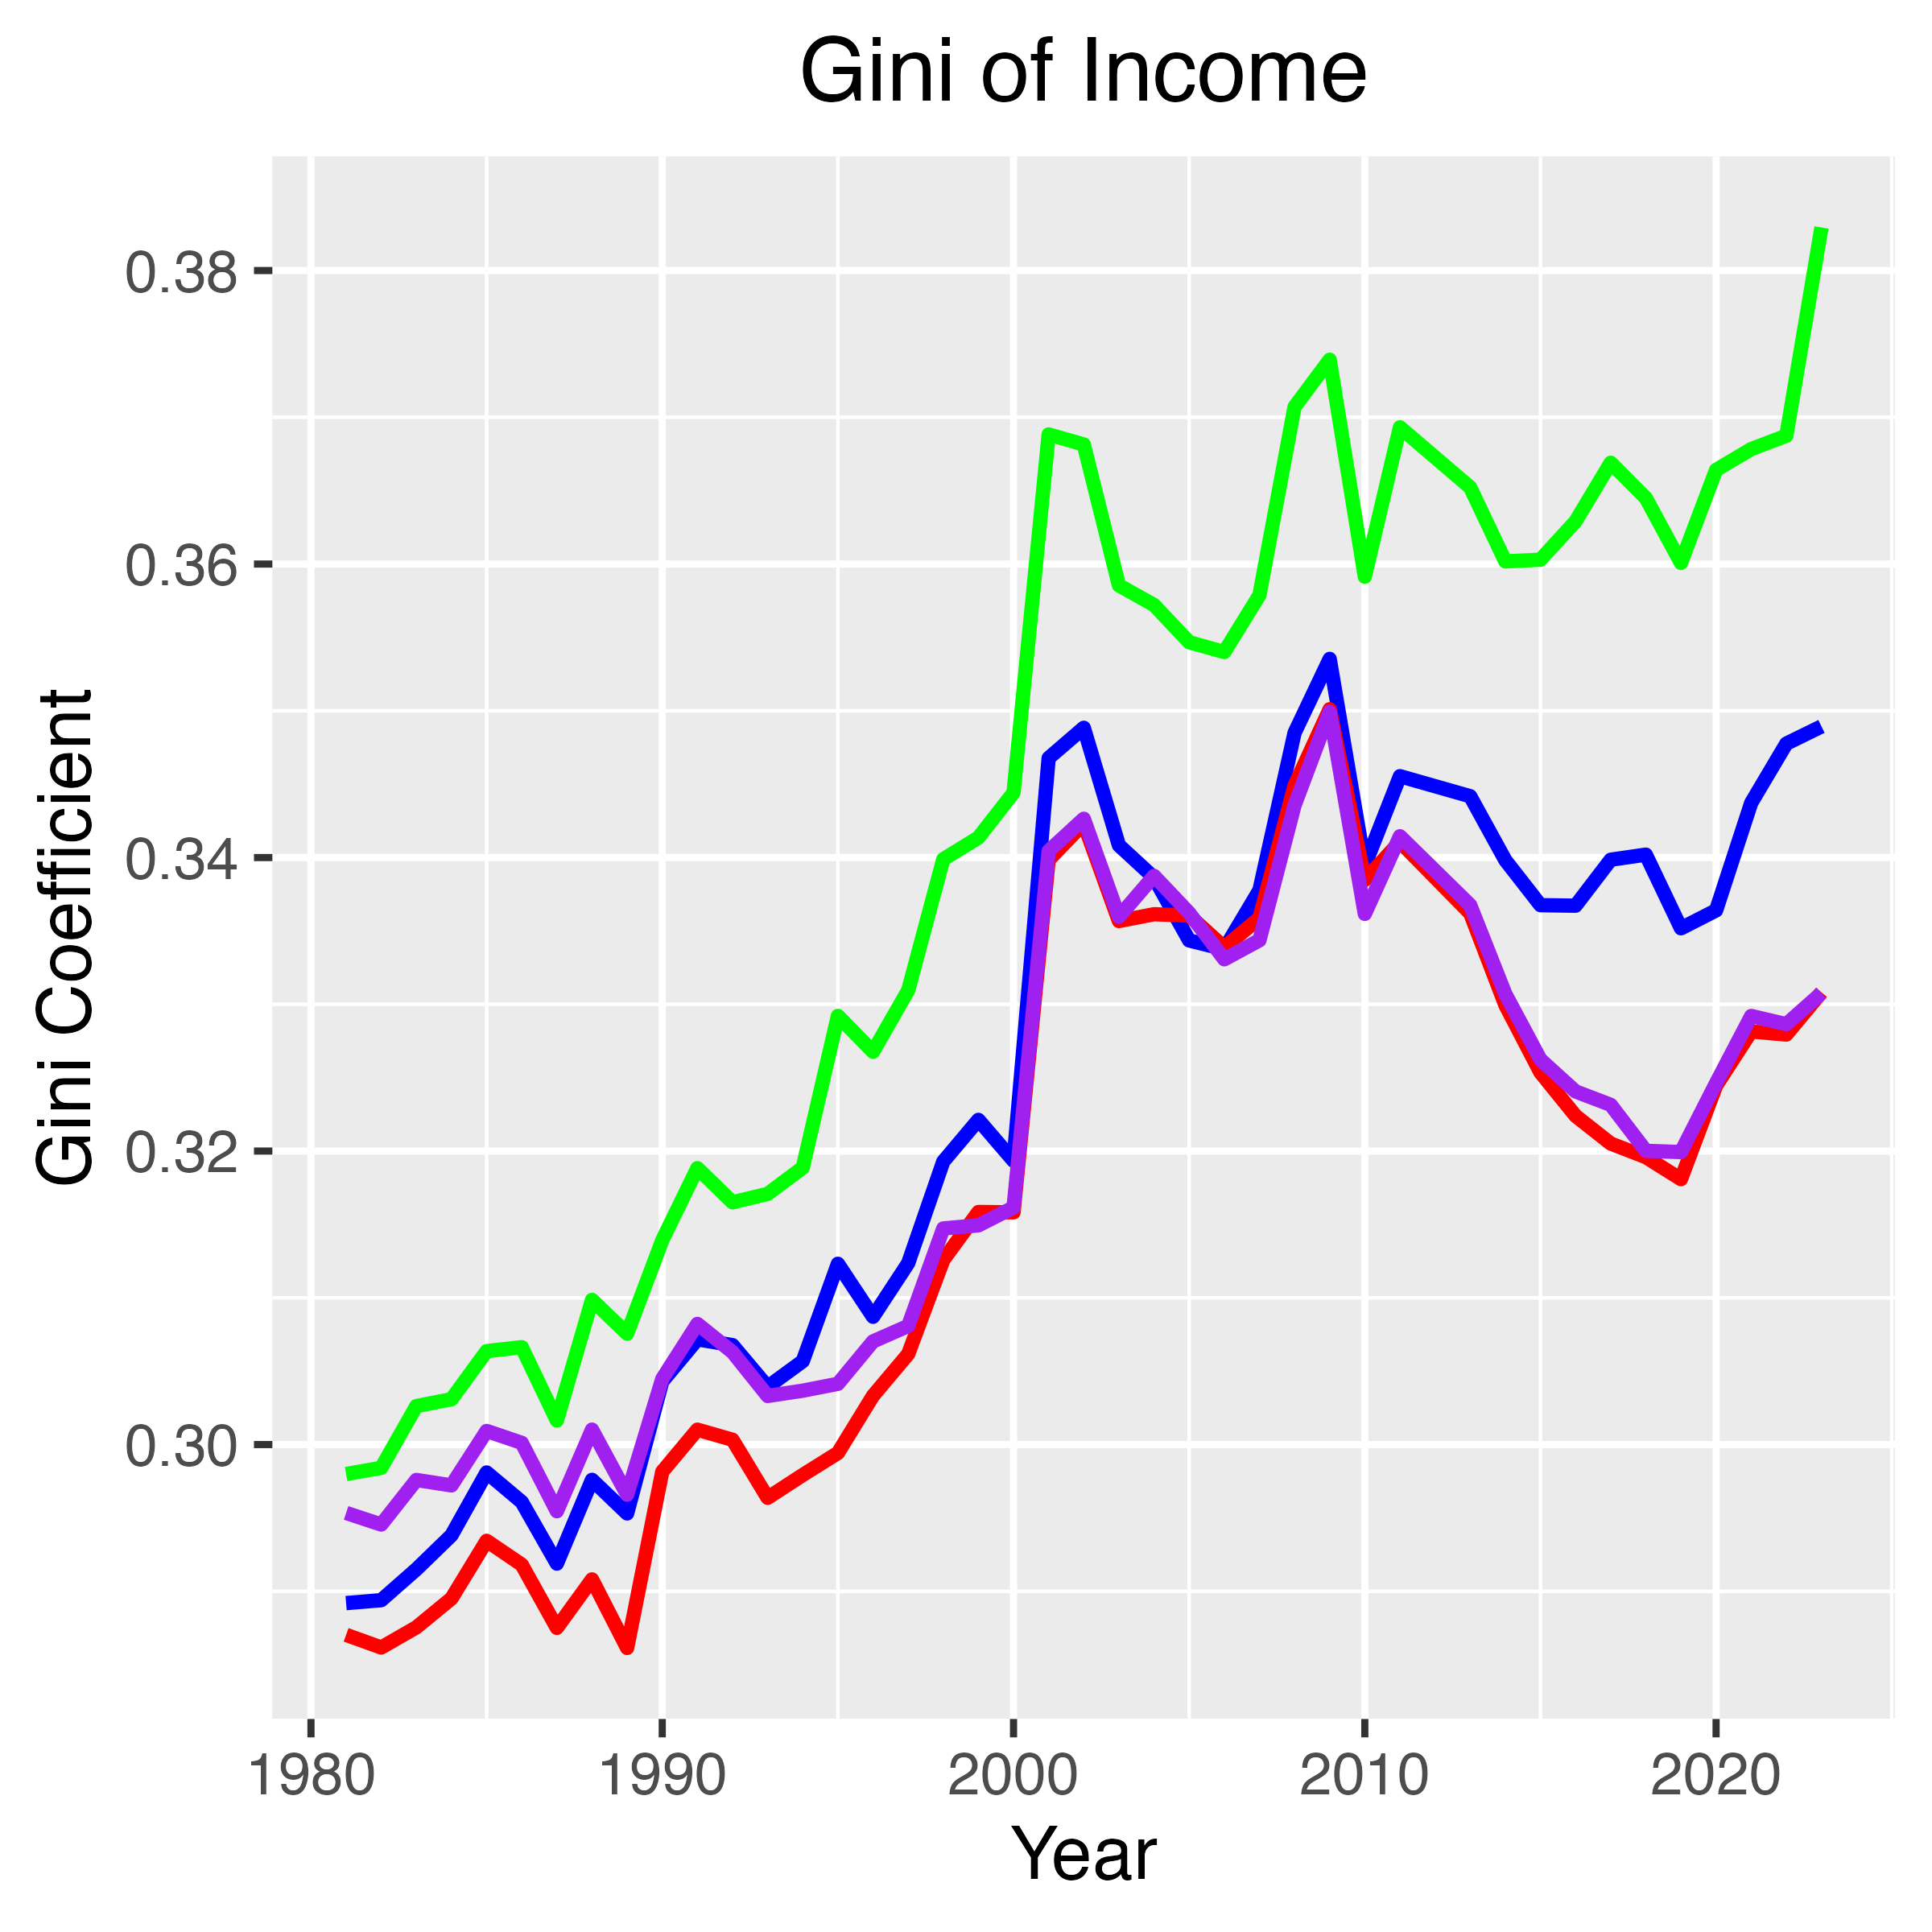
\includegraphics[width=\textwidth]{figures/Fig_4/Fig_4b_Gini_inc.png}
    \end{subfigure}
    \begin{subfigure}[t]{0.475\textwidth}
        \centering
        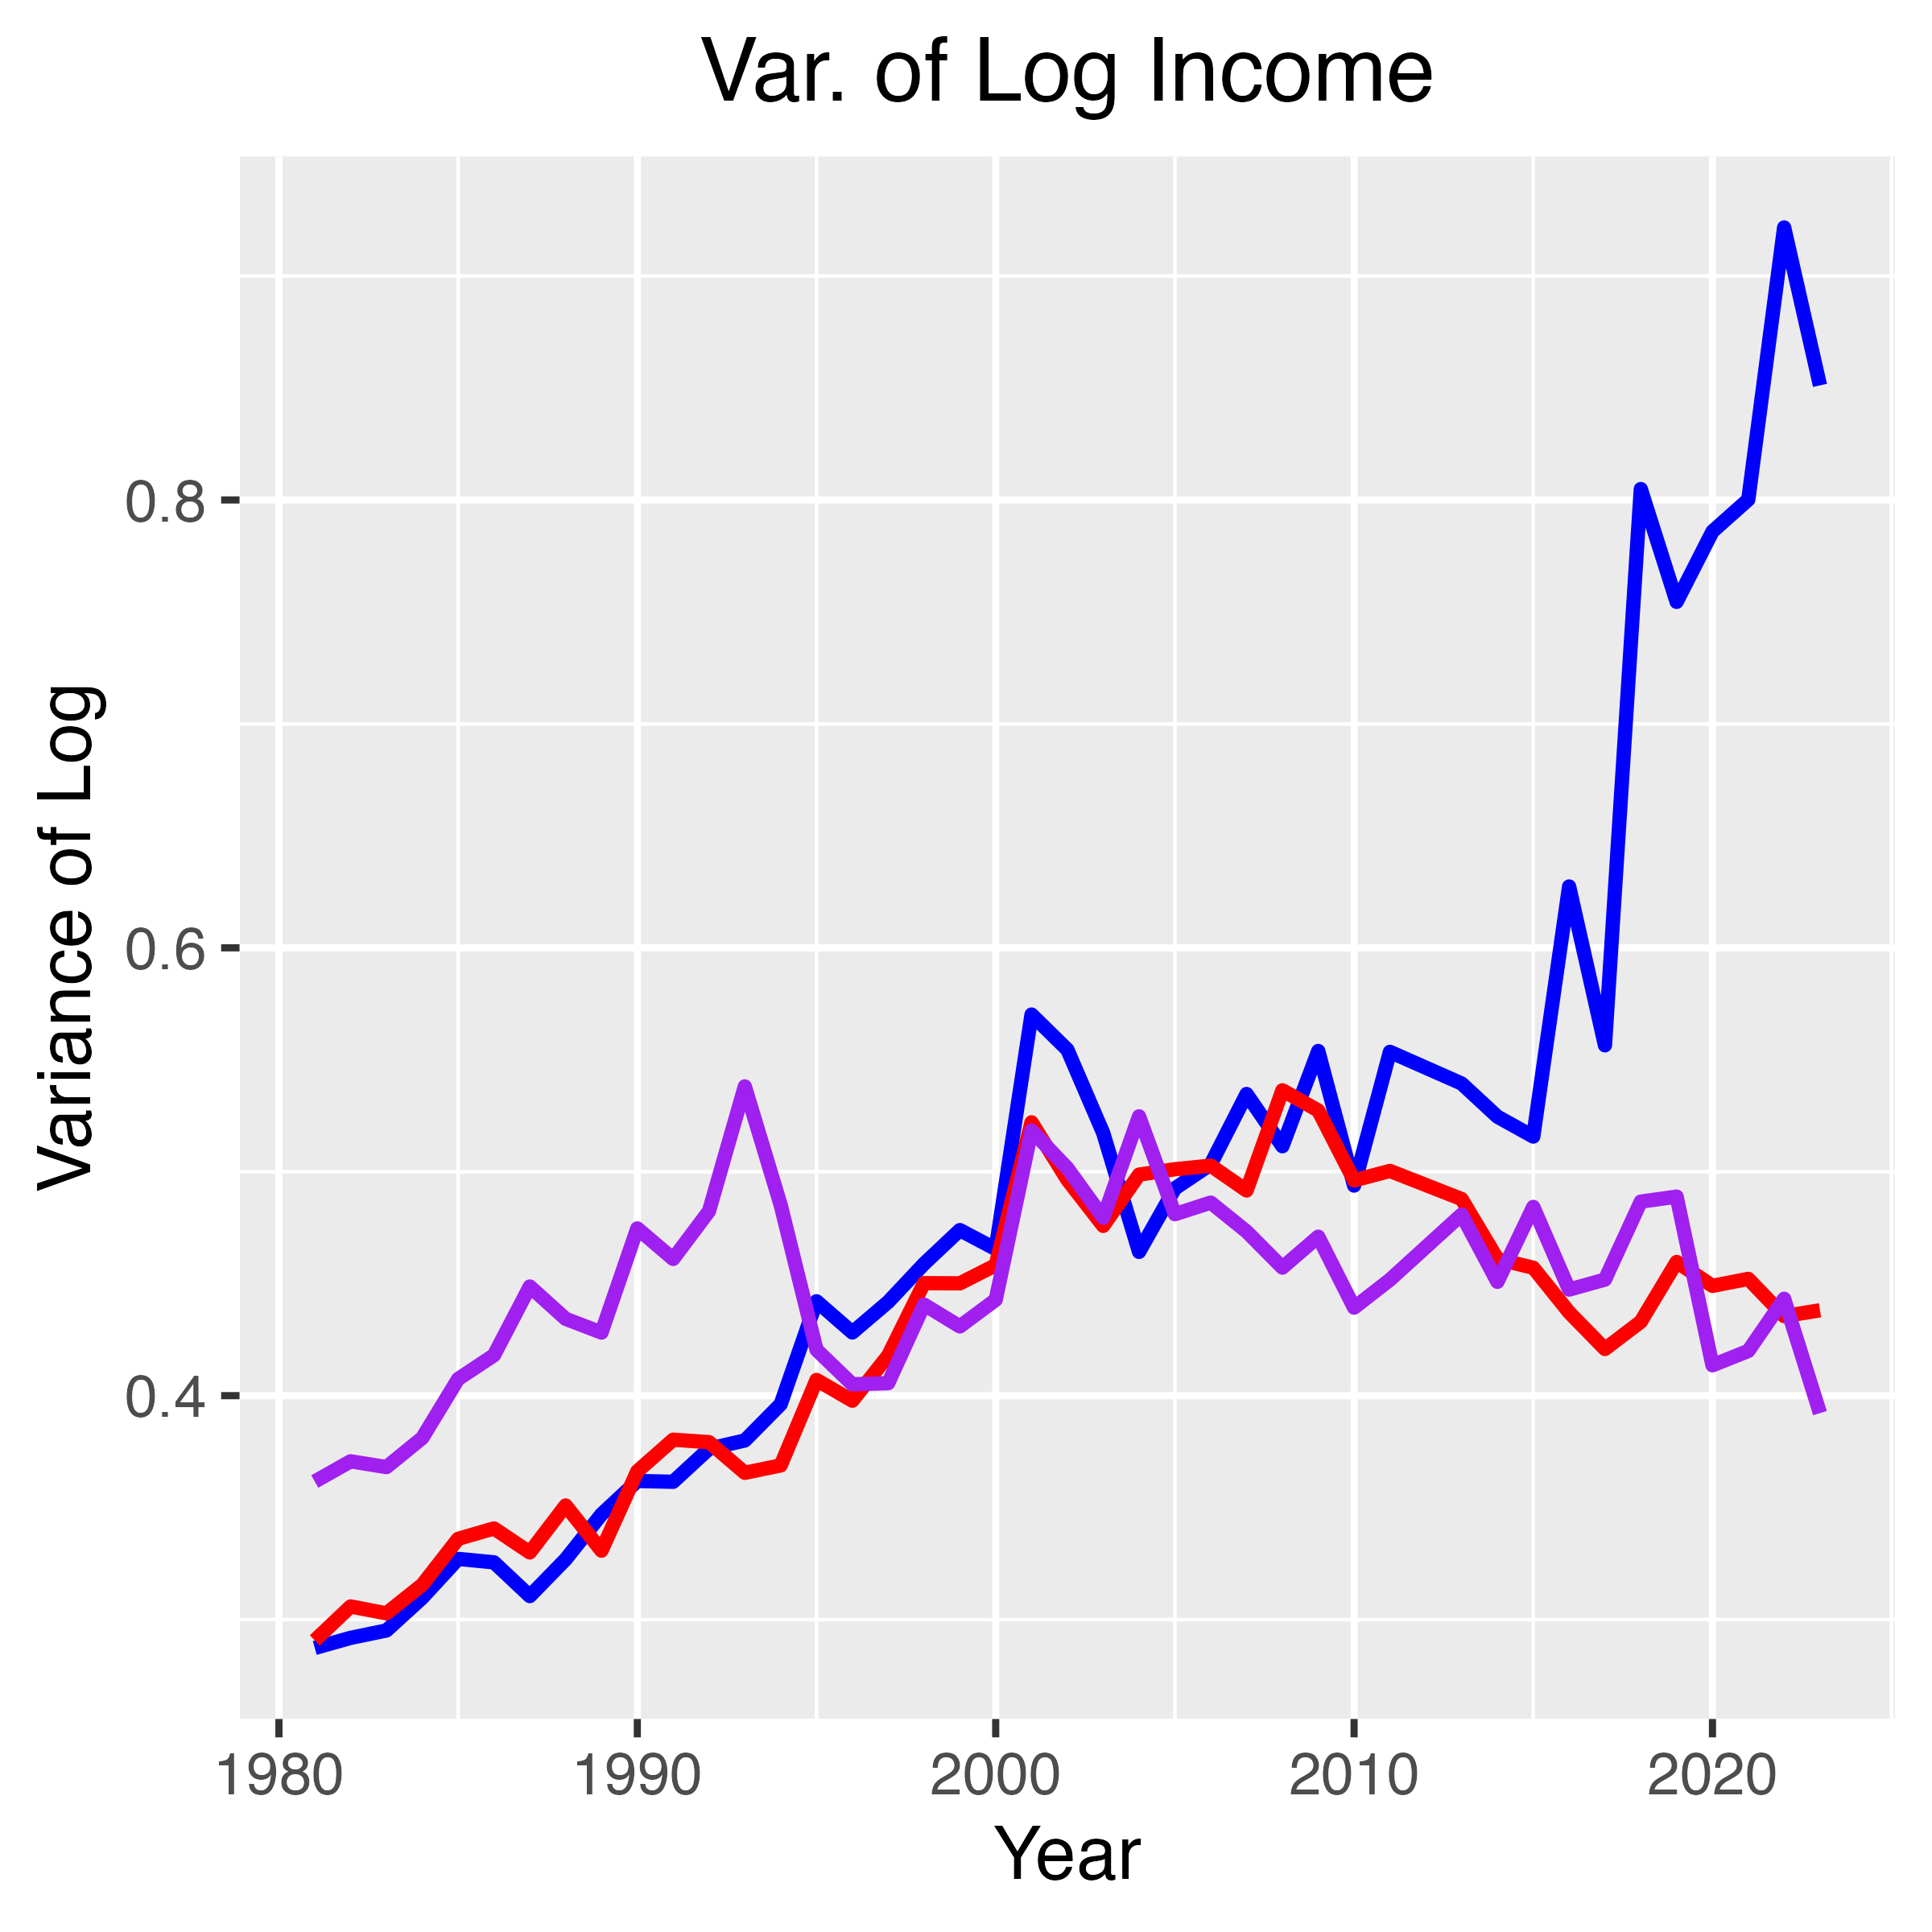
\includegraphics[width=\textwidth]{figures/Fig_4/Fig_4c_Var_inc.png}
    \end{subfigure}
    \begin{subfigure}[t]{0.475\textwidth}
        \centering
        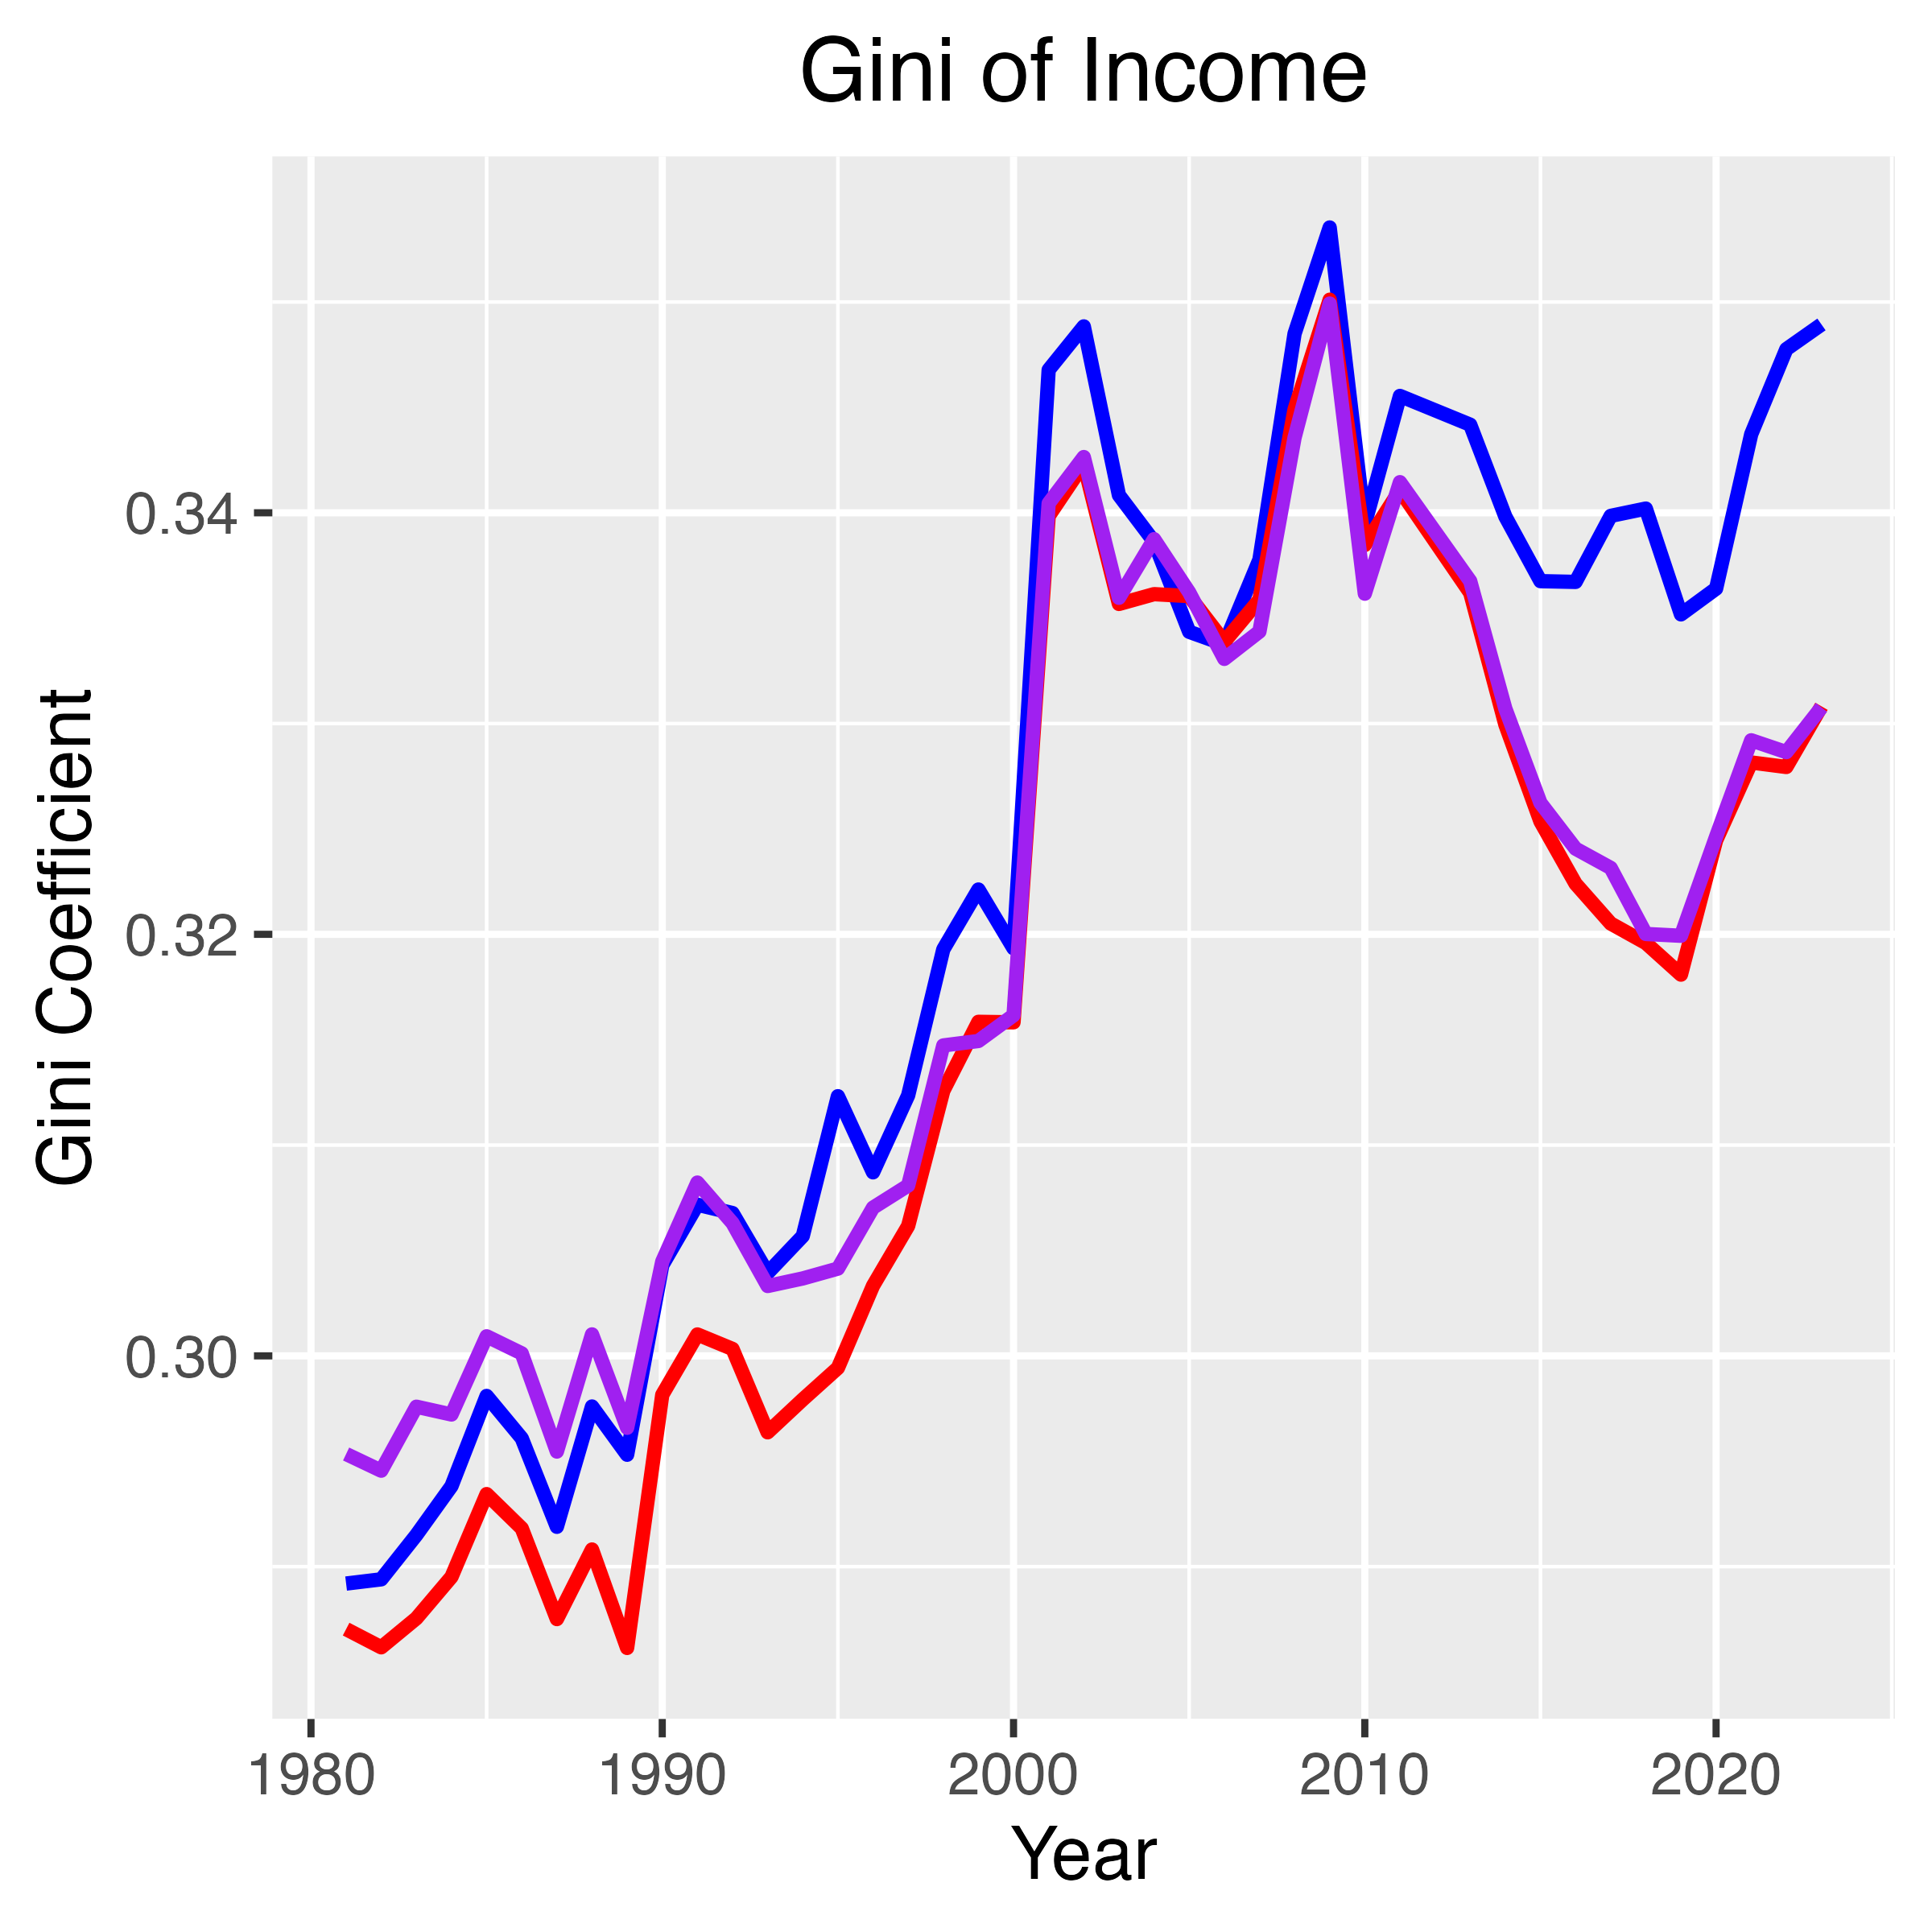
\includegraphics[width=\textwidth]{figures/Fig_4/Fig_4d_Gini_inc.png}
    \end{subfigure}
    \caption{From Household Earnings to Pre-Government Income}
    \label{fig:Trans_Asset}
\end{figure}

In Figure \ref{fig:Trans_Asset}, we discuss income sources beyond earnings, including asset income and private transfers. Each line covers the households whose value of that aggregate passes the threshold in Section \ref{sec:sample}, so the lines that add asset income or private transfers also include households without earnings. 

Asset income increases inequality while private transfers reduce it. Adding asset income raises the Gini coefficient and the variance of logs in every year. Among households in the earnings sample alone, adding asset income raises the Gini by only 0.002 to 0.008. Thus, from 1992 onward, most of the increase in the measures comes from households without earnings entering the sample. Adding private transfers to earnings plus asset income lowers both measures in every year. For transfers to lower inequality in this way, they must make up a larger share of income for households with low earnings than for those with high earnings.
This pattern is consistent with the idea that beyond the household, the family or clan can smooth out income shocks using private transfers. 

The two components are also nearly unrelated. Among households with either a private transfer or asset income, the correlation between the two amounts lies between $0.00$ and $0.08$ in every year (Appendix Figure \ref{fig:appendix_corr}), so larger transfers do not go systematically to households with more asset income.

\begin{figure}[t]
    \centering
    \begin{subfigure}[t]{0.475\textwidth}
        \centering
        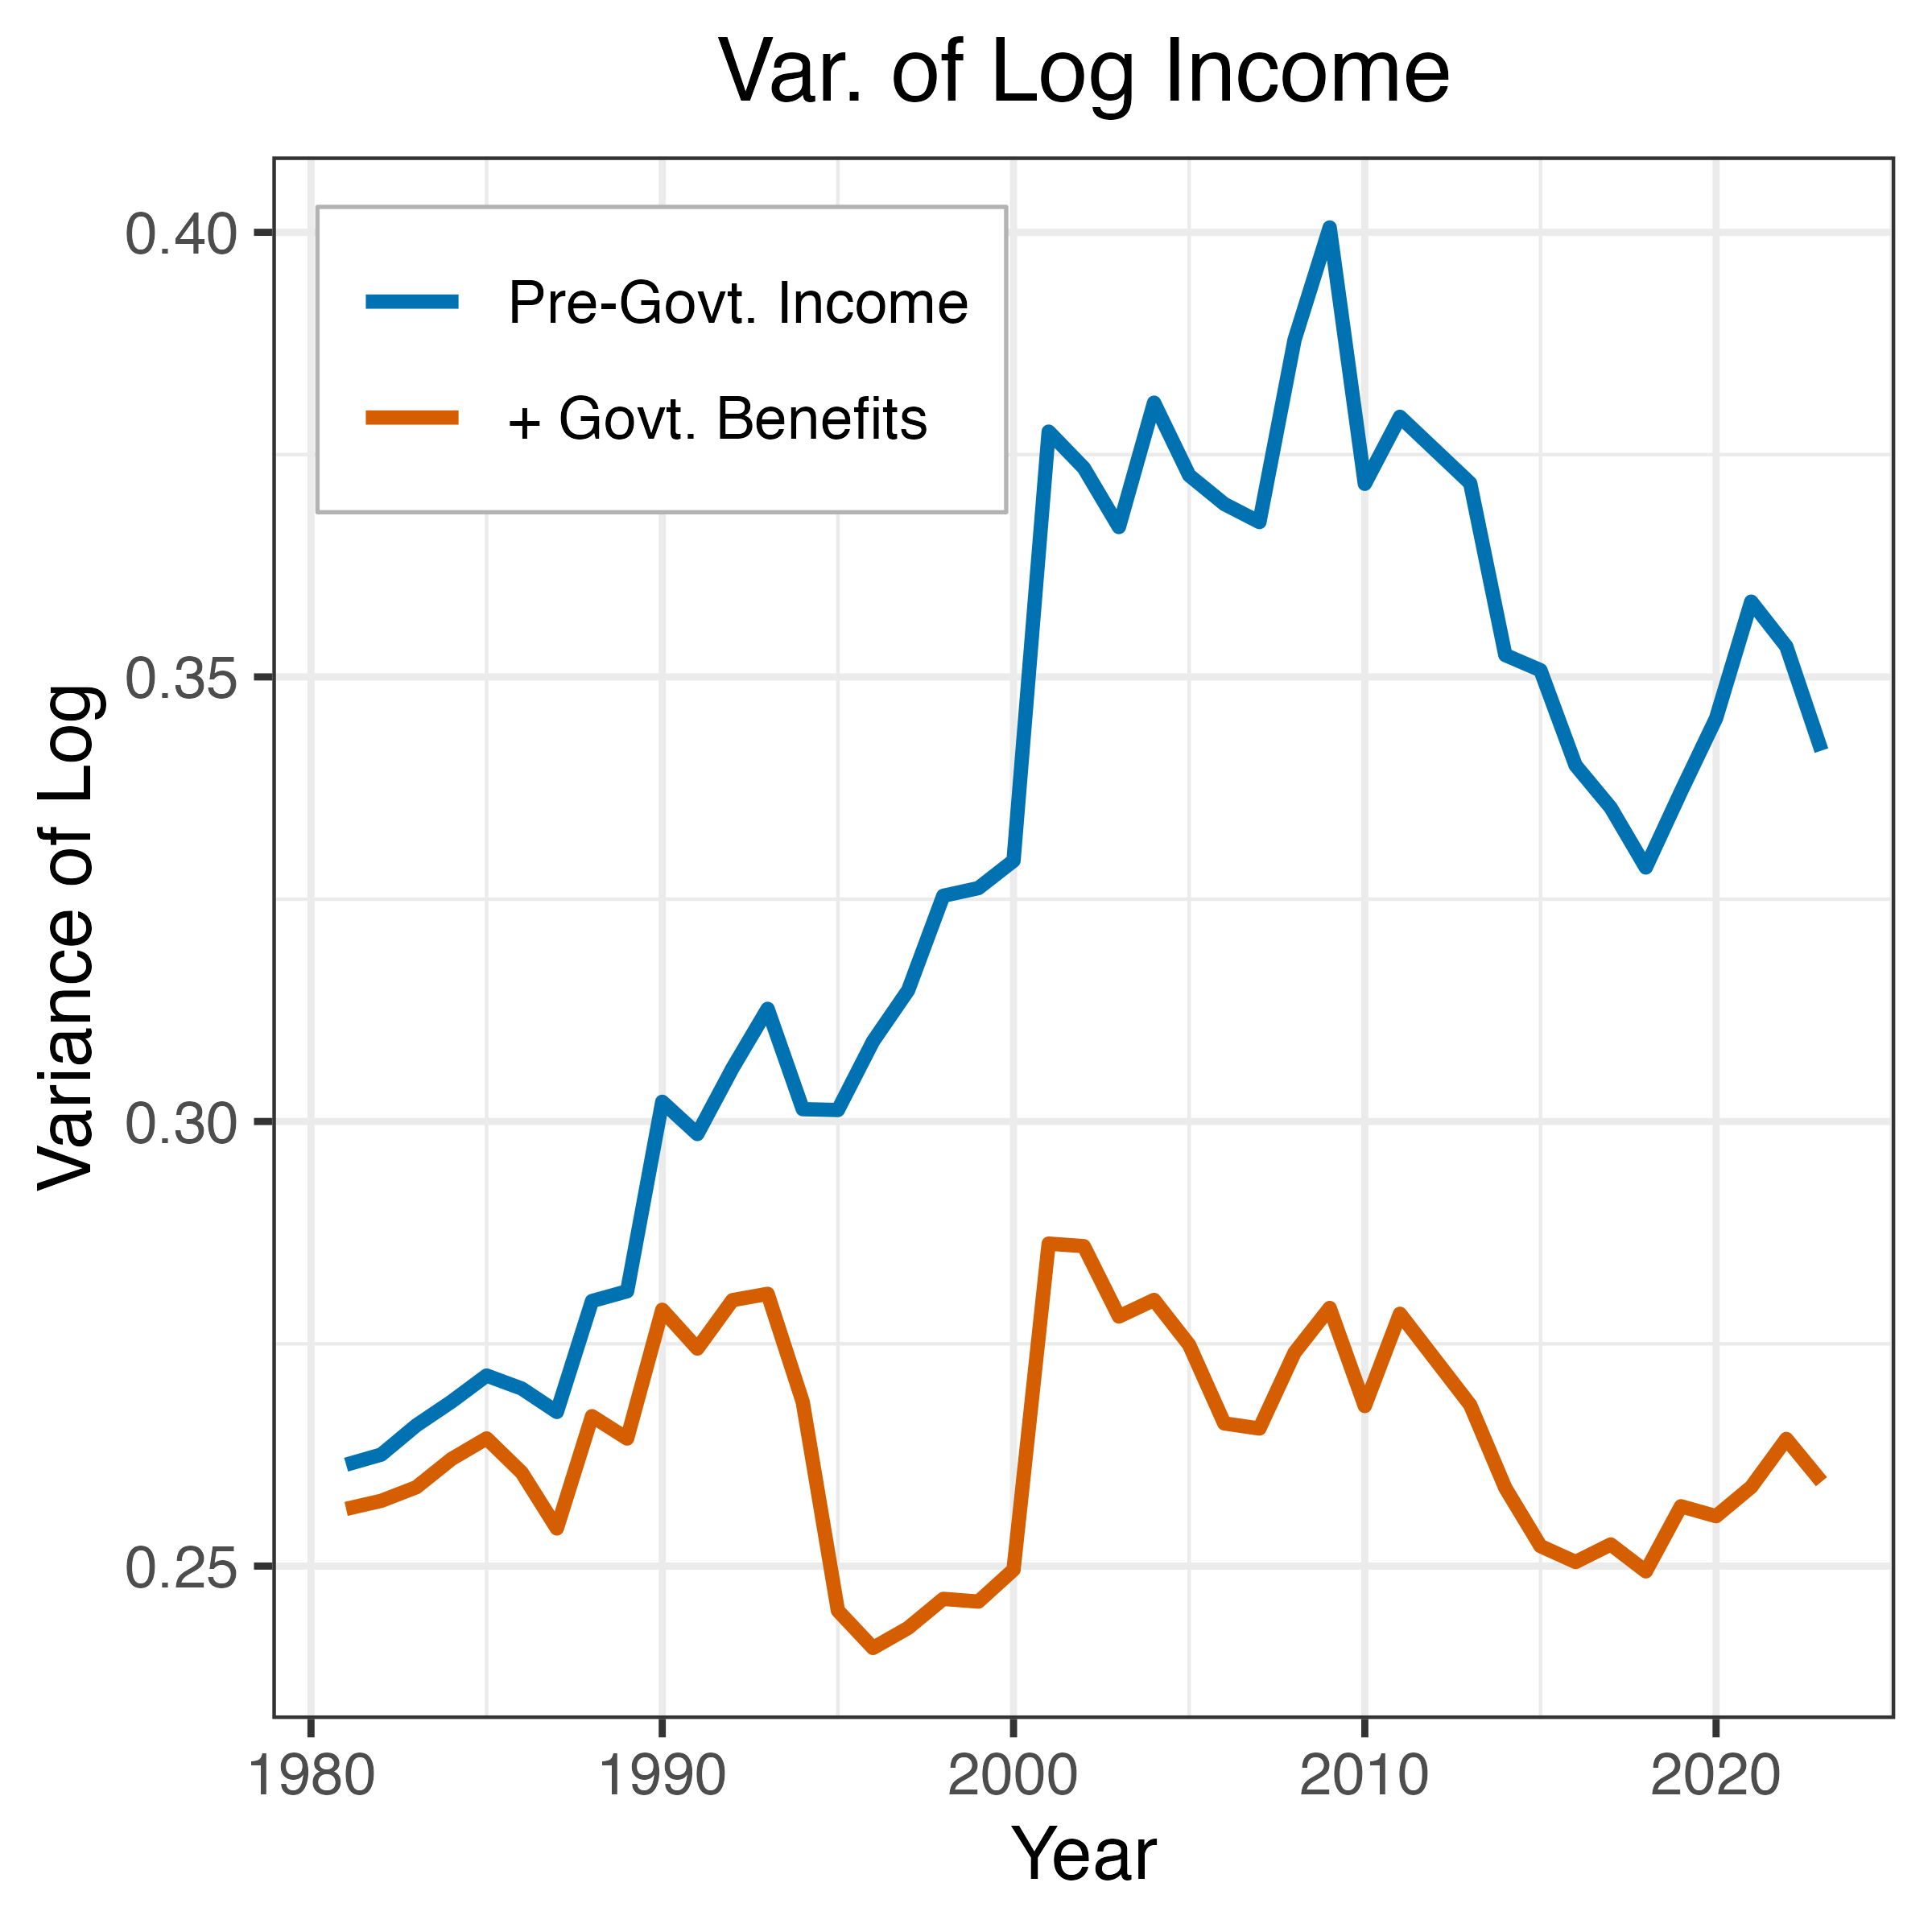
\includegraphics[width=\textwidth]{figures/Fig_5/Fig_5a_Var_inc.png}
    \end{subfigure}
    \begin{subfigure}[t]{0.475\textwidth}
        \centering
        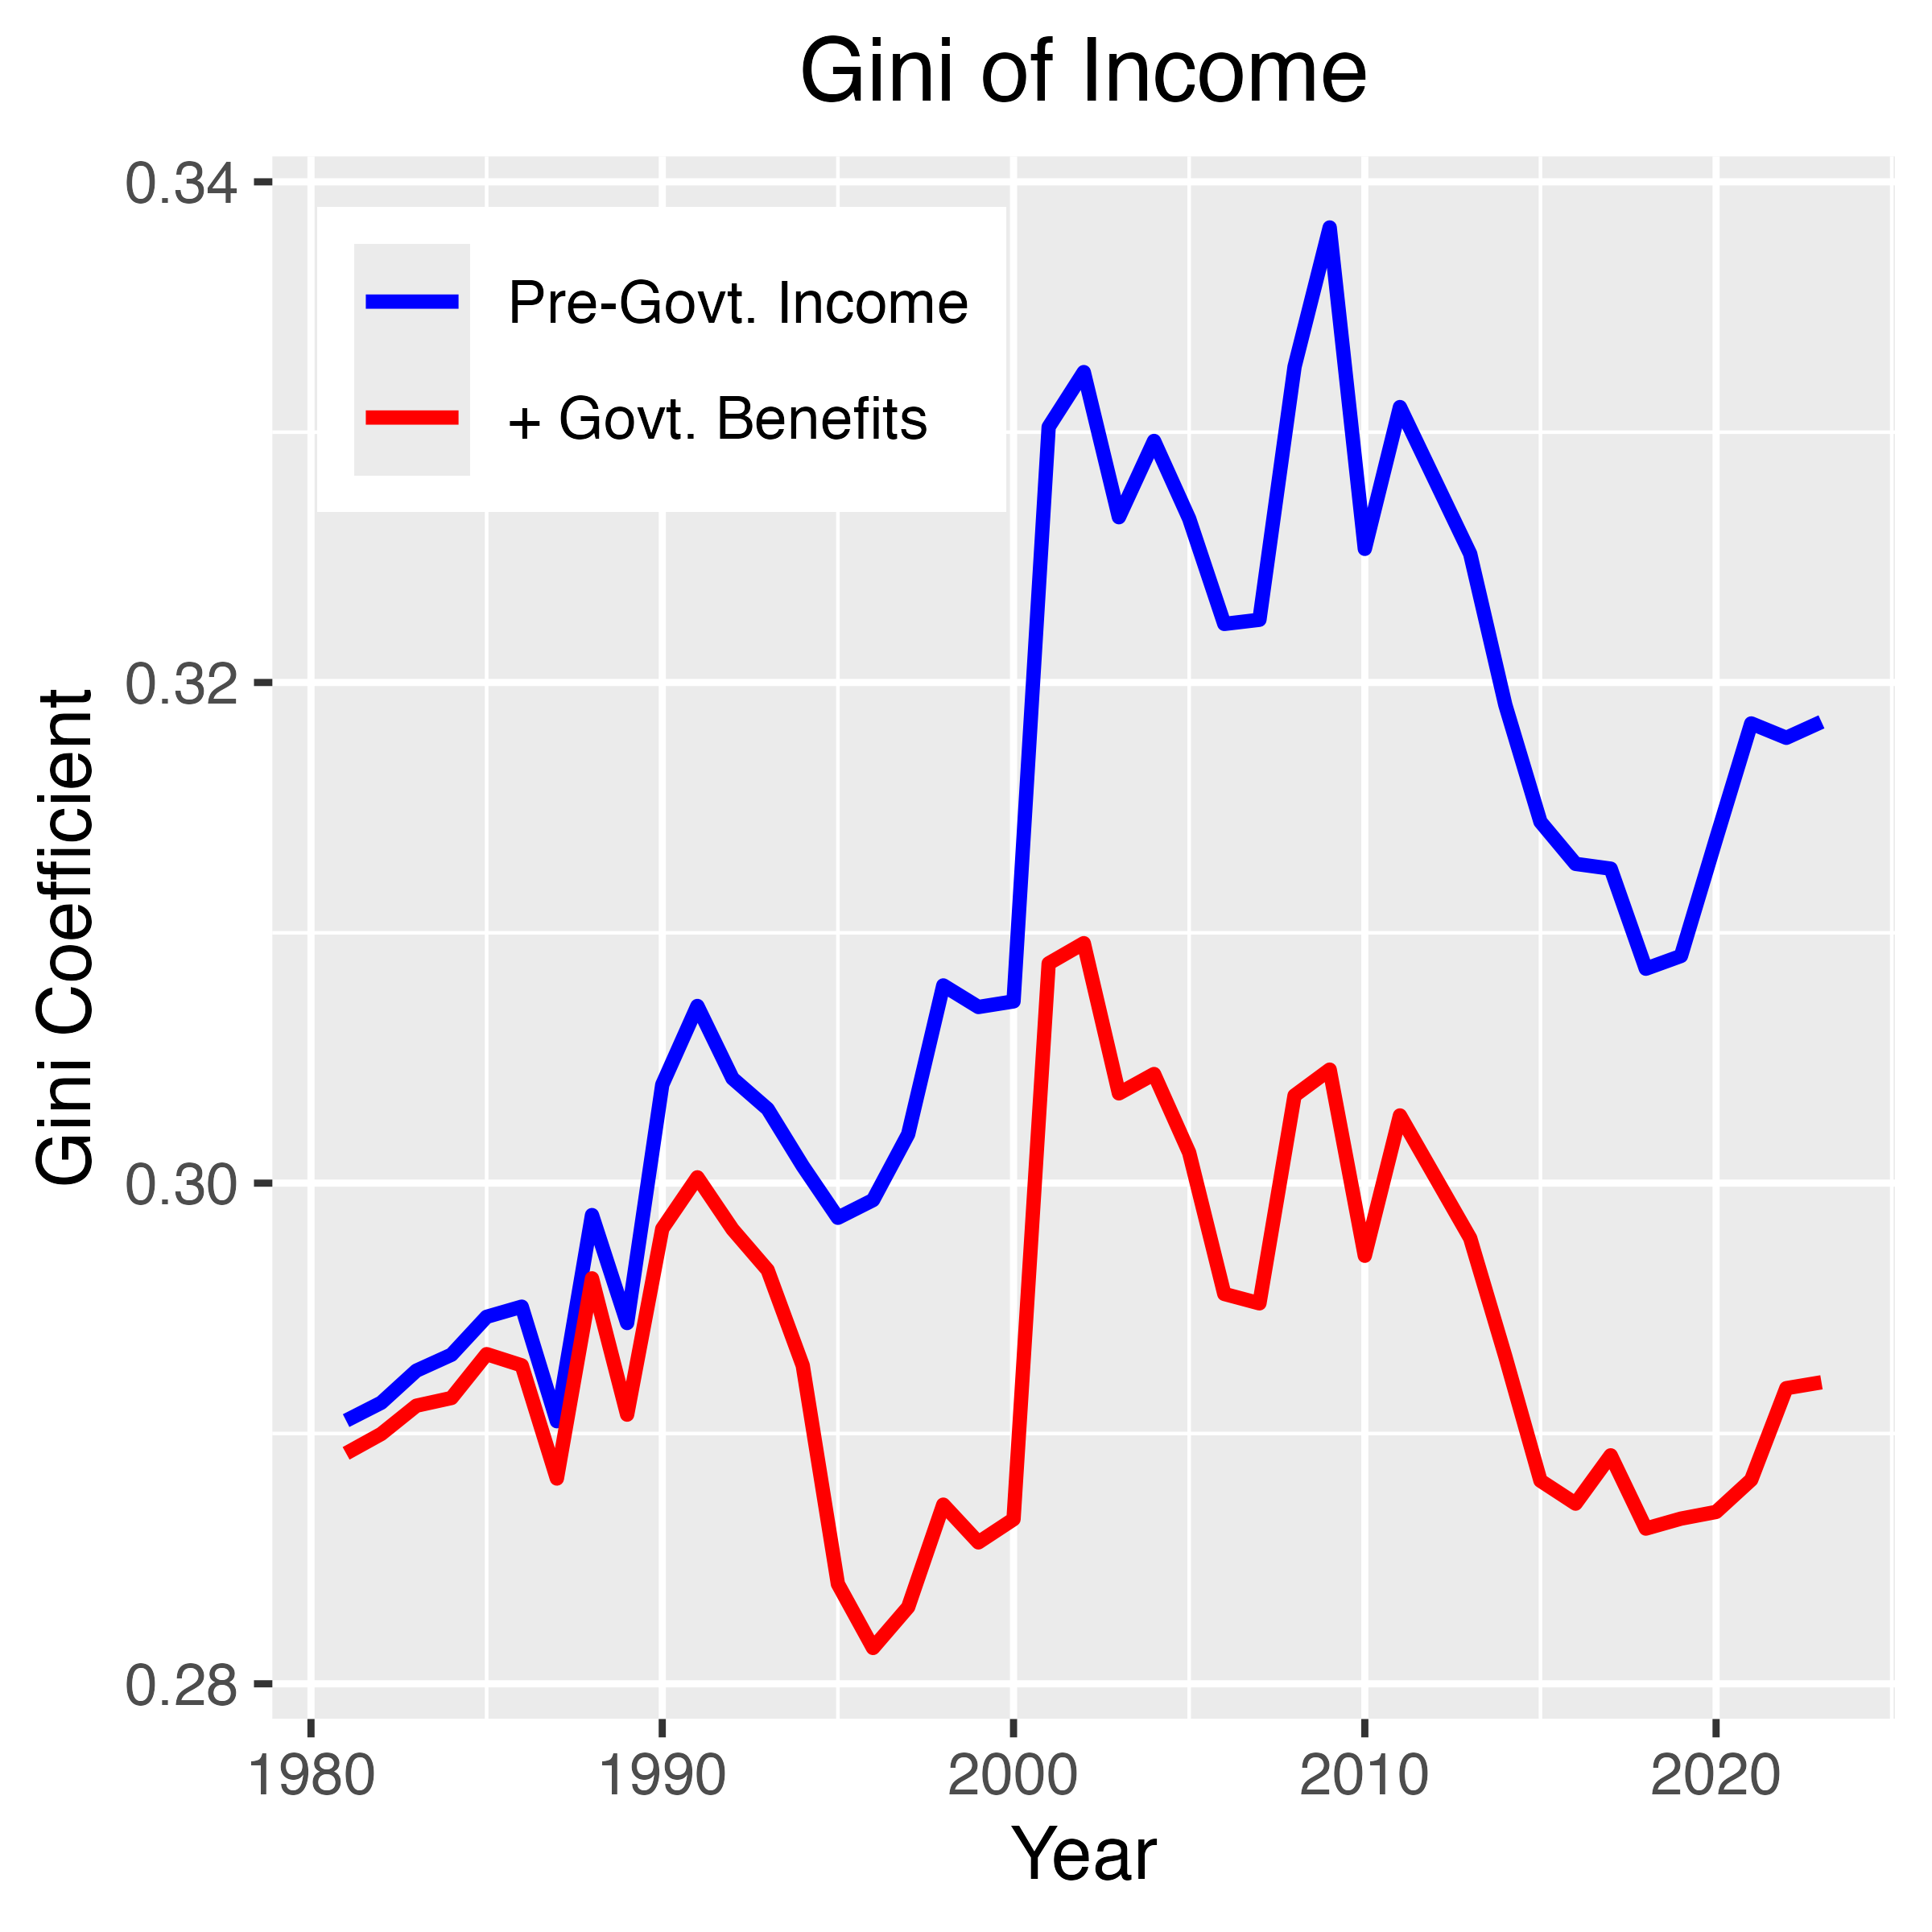
\includegraphics[width=\textwidth]{figures/Fig_5/Fig_5b_Gini_inc.png}
    \end{subfigure}
    \begin{subfigure}[t]{0.475\textwidth}
        \centering
        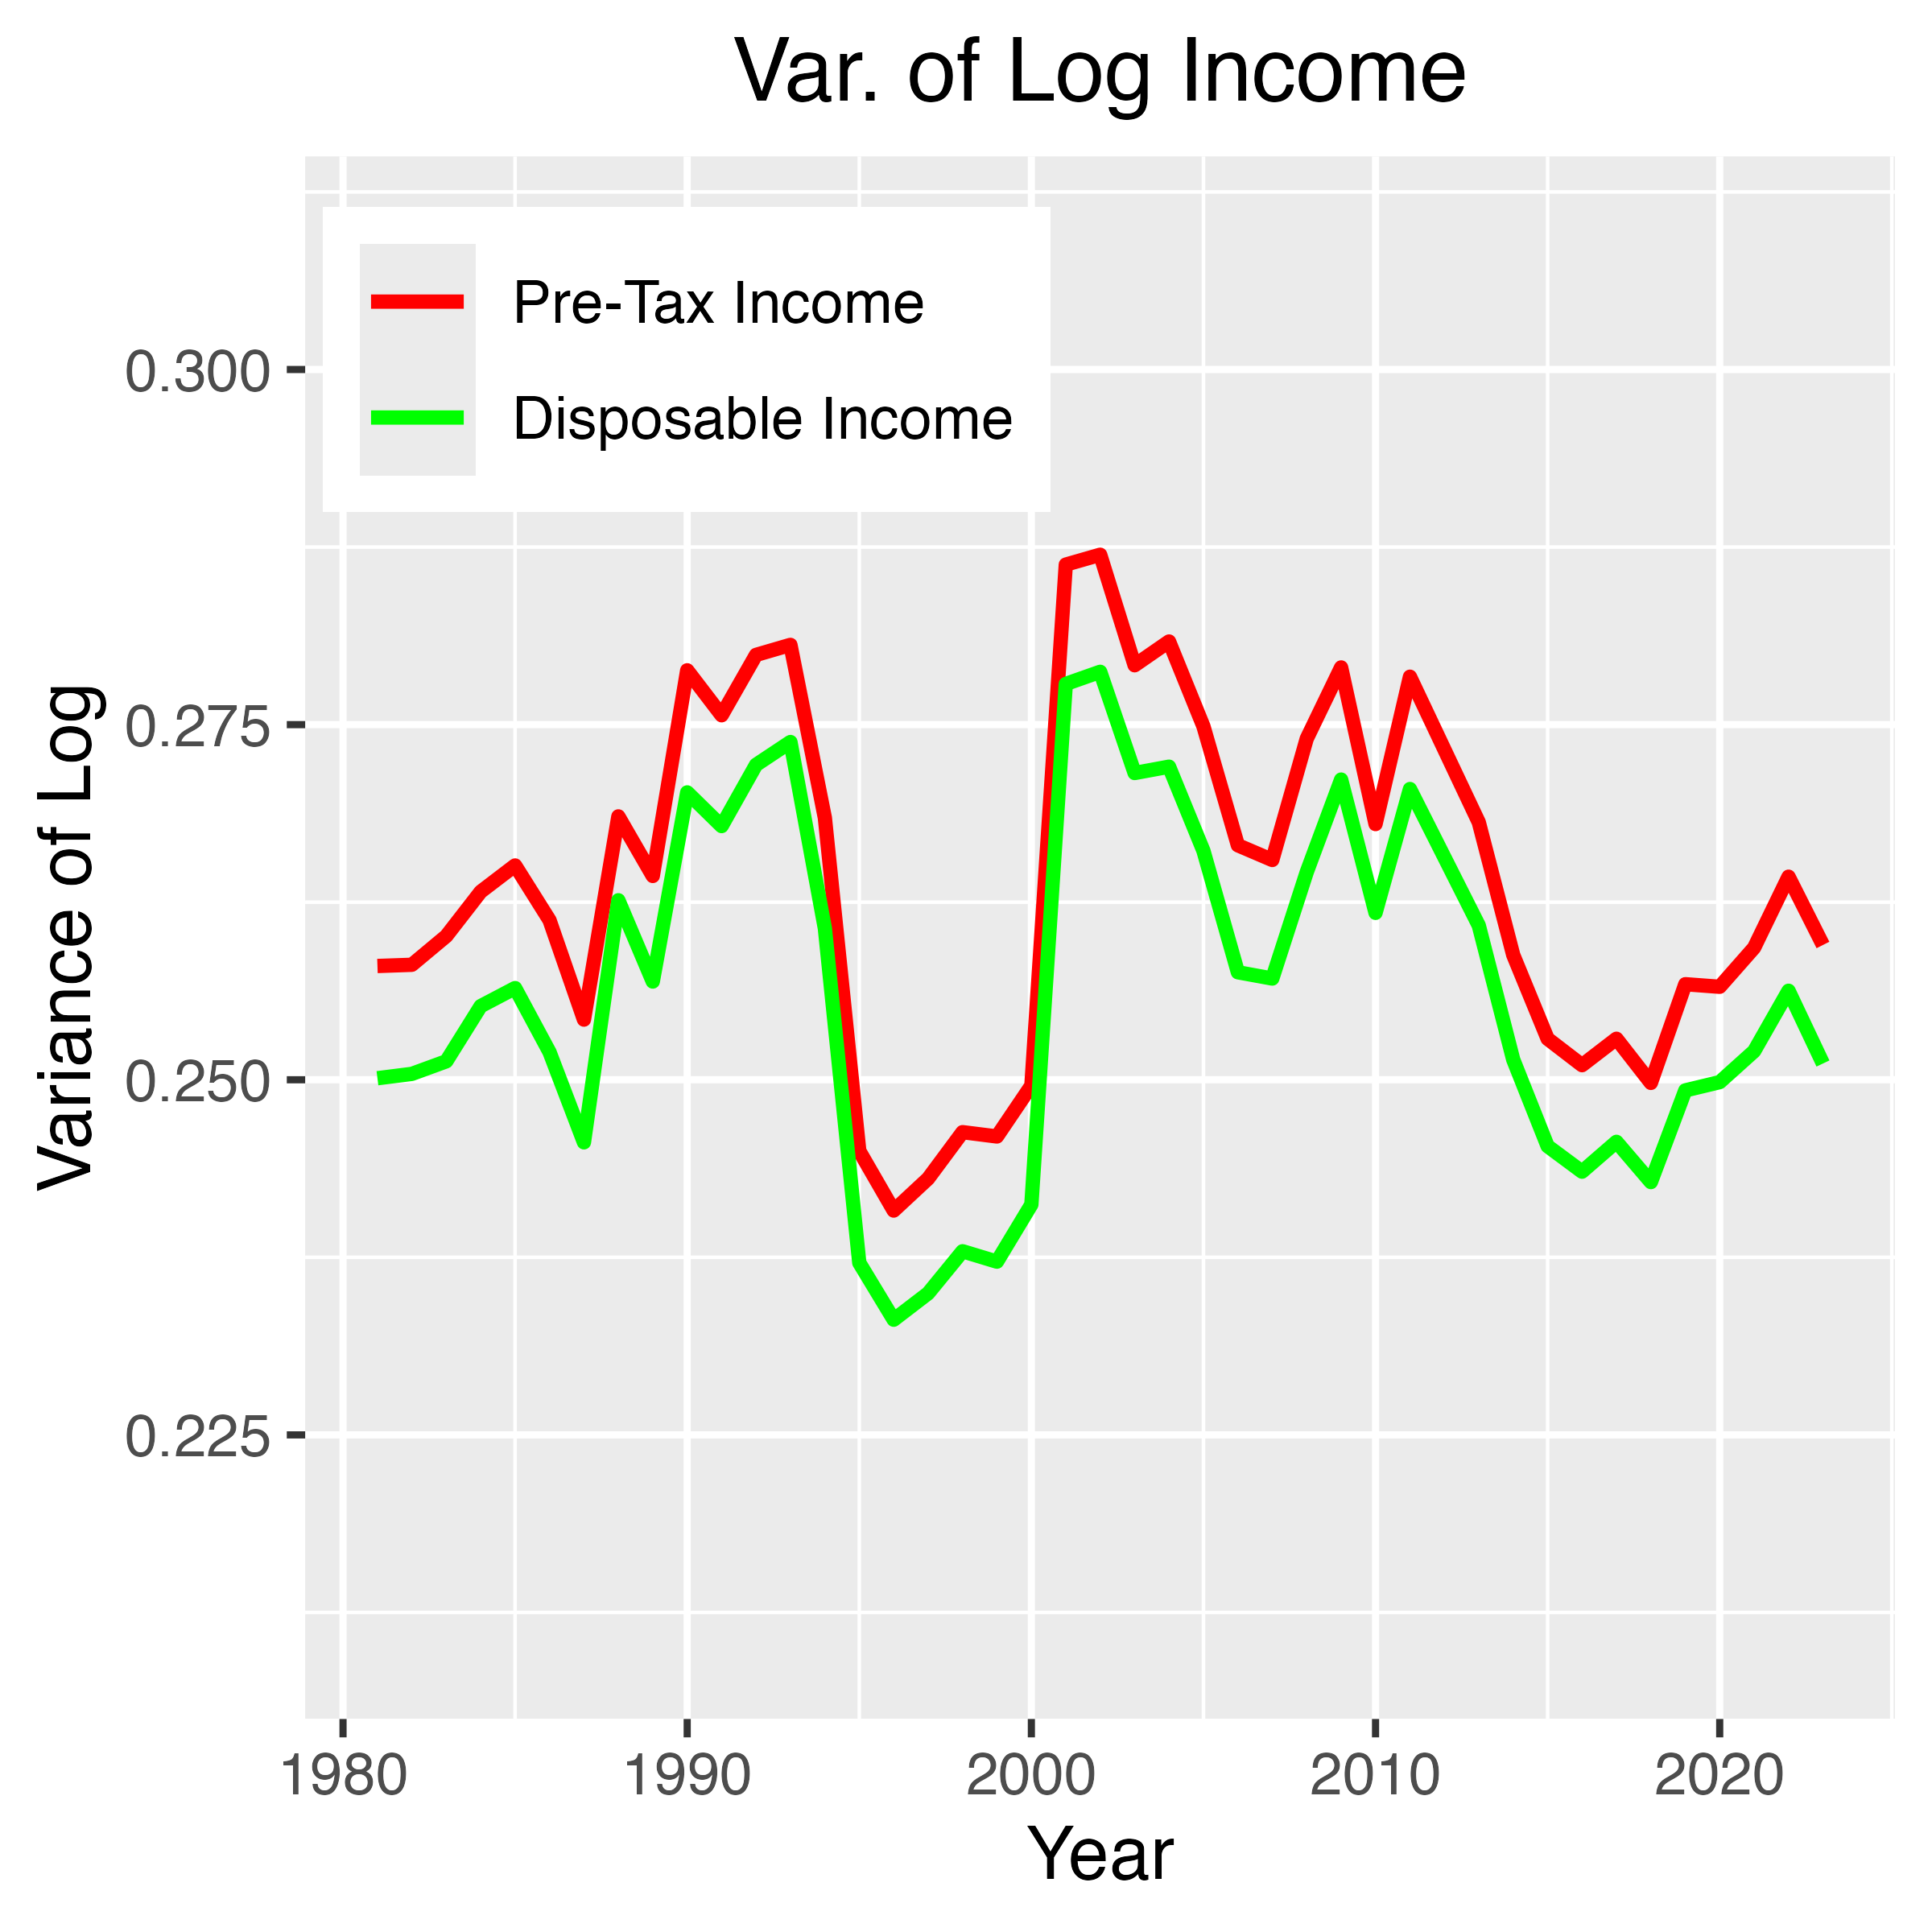
\includegraphics[width=\textwidth]{figures/Fig_5/Fig_5c_Var_inc.png}
    \end{subfigure}
    \begin{subfigure}[t]{0.475\textwidth}
        \centering
        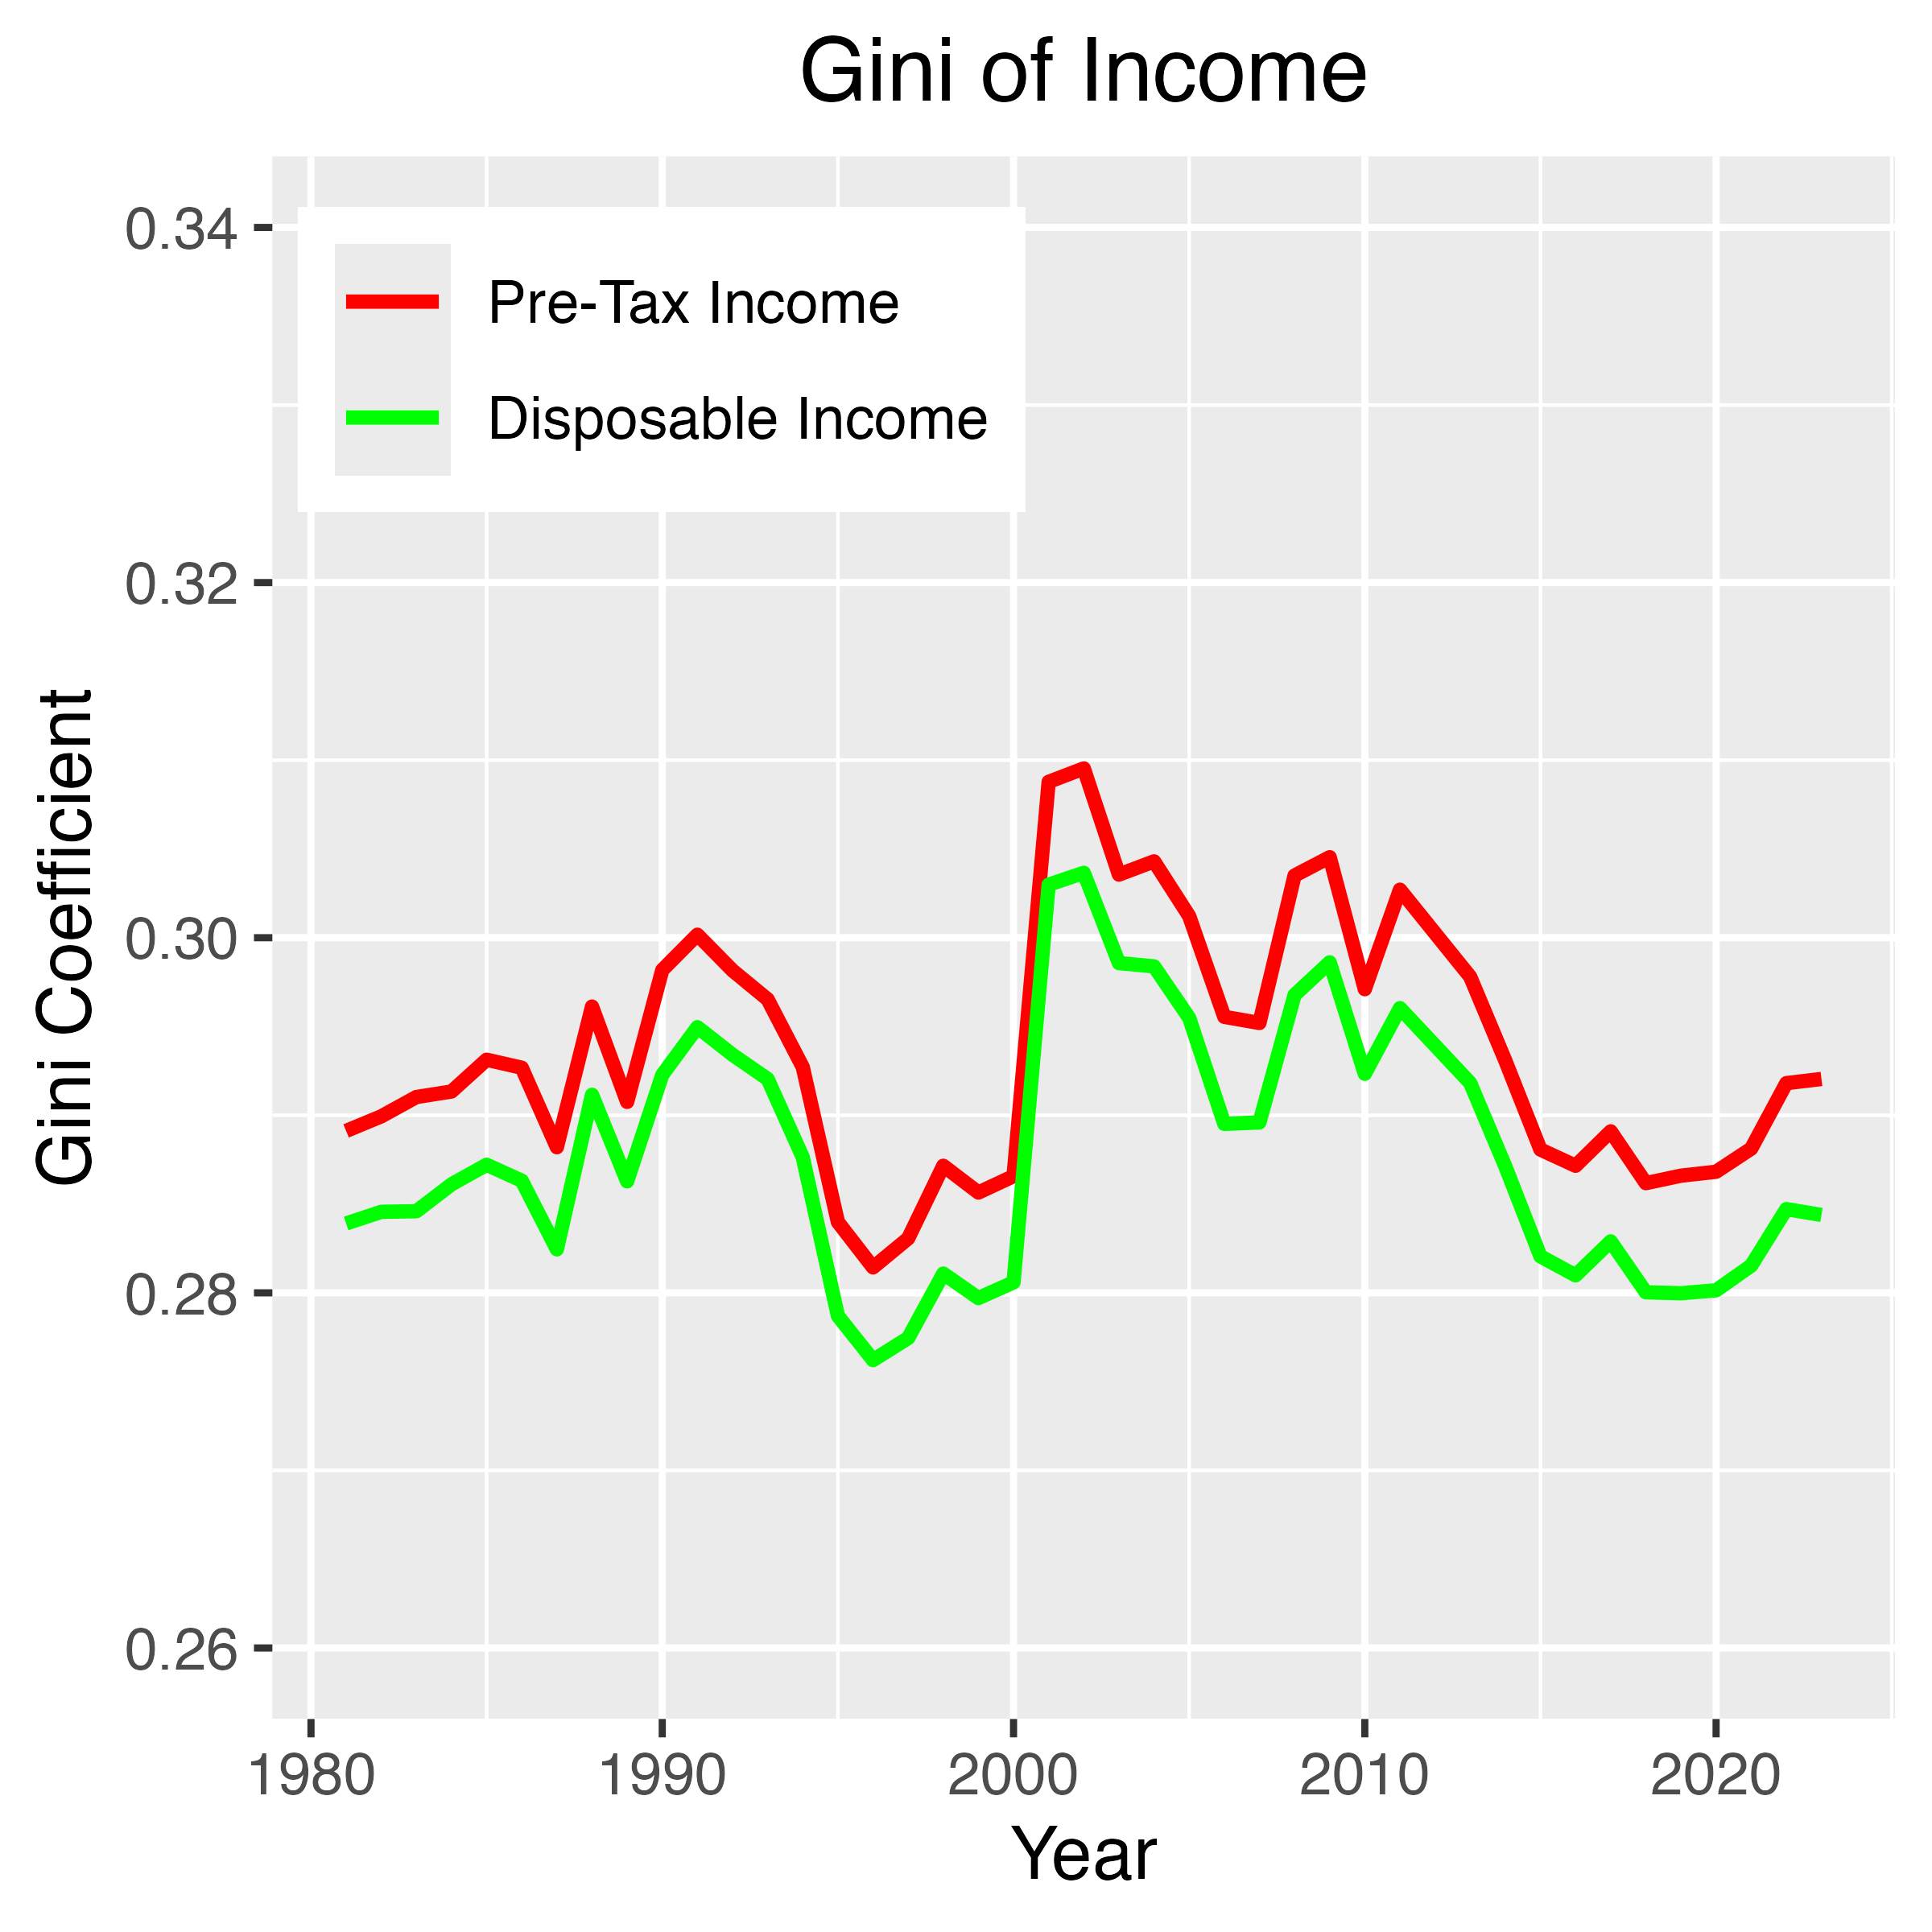
\includegraphics[width=\textwidth]{figures/Fig_5/Fig_5d_Gini_inc.png}
    \end{subfigure}
    \caption{From Pre-Government to Disposable Income}
    \label{fig:Gov}
\end{figure}

\begin{figure}[htbp]
    \centering
    \begin{subfigure}[t]{0.475\textwidth}
        \centering
        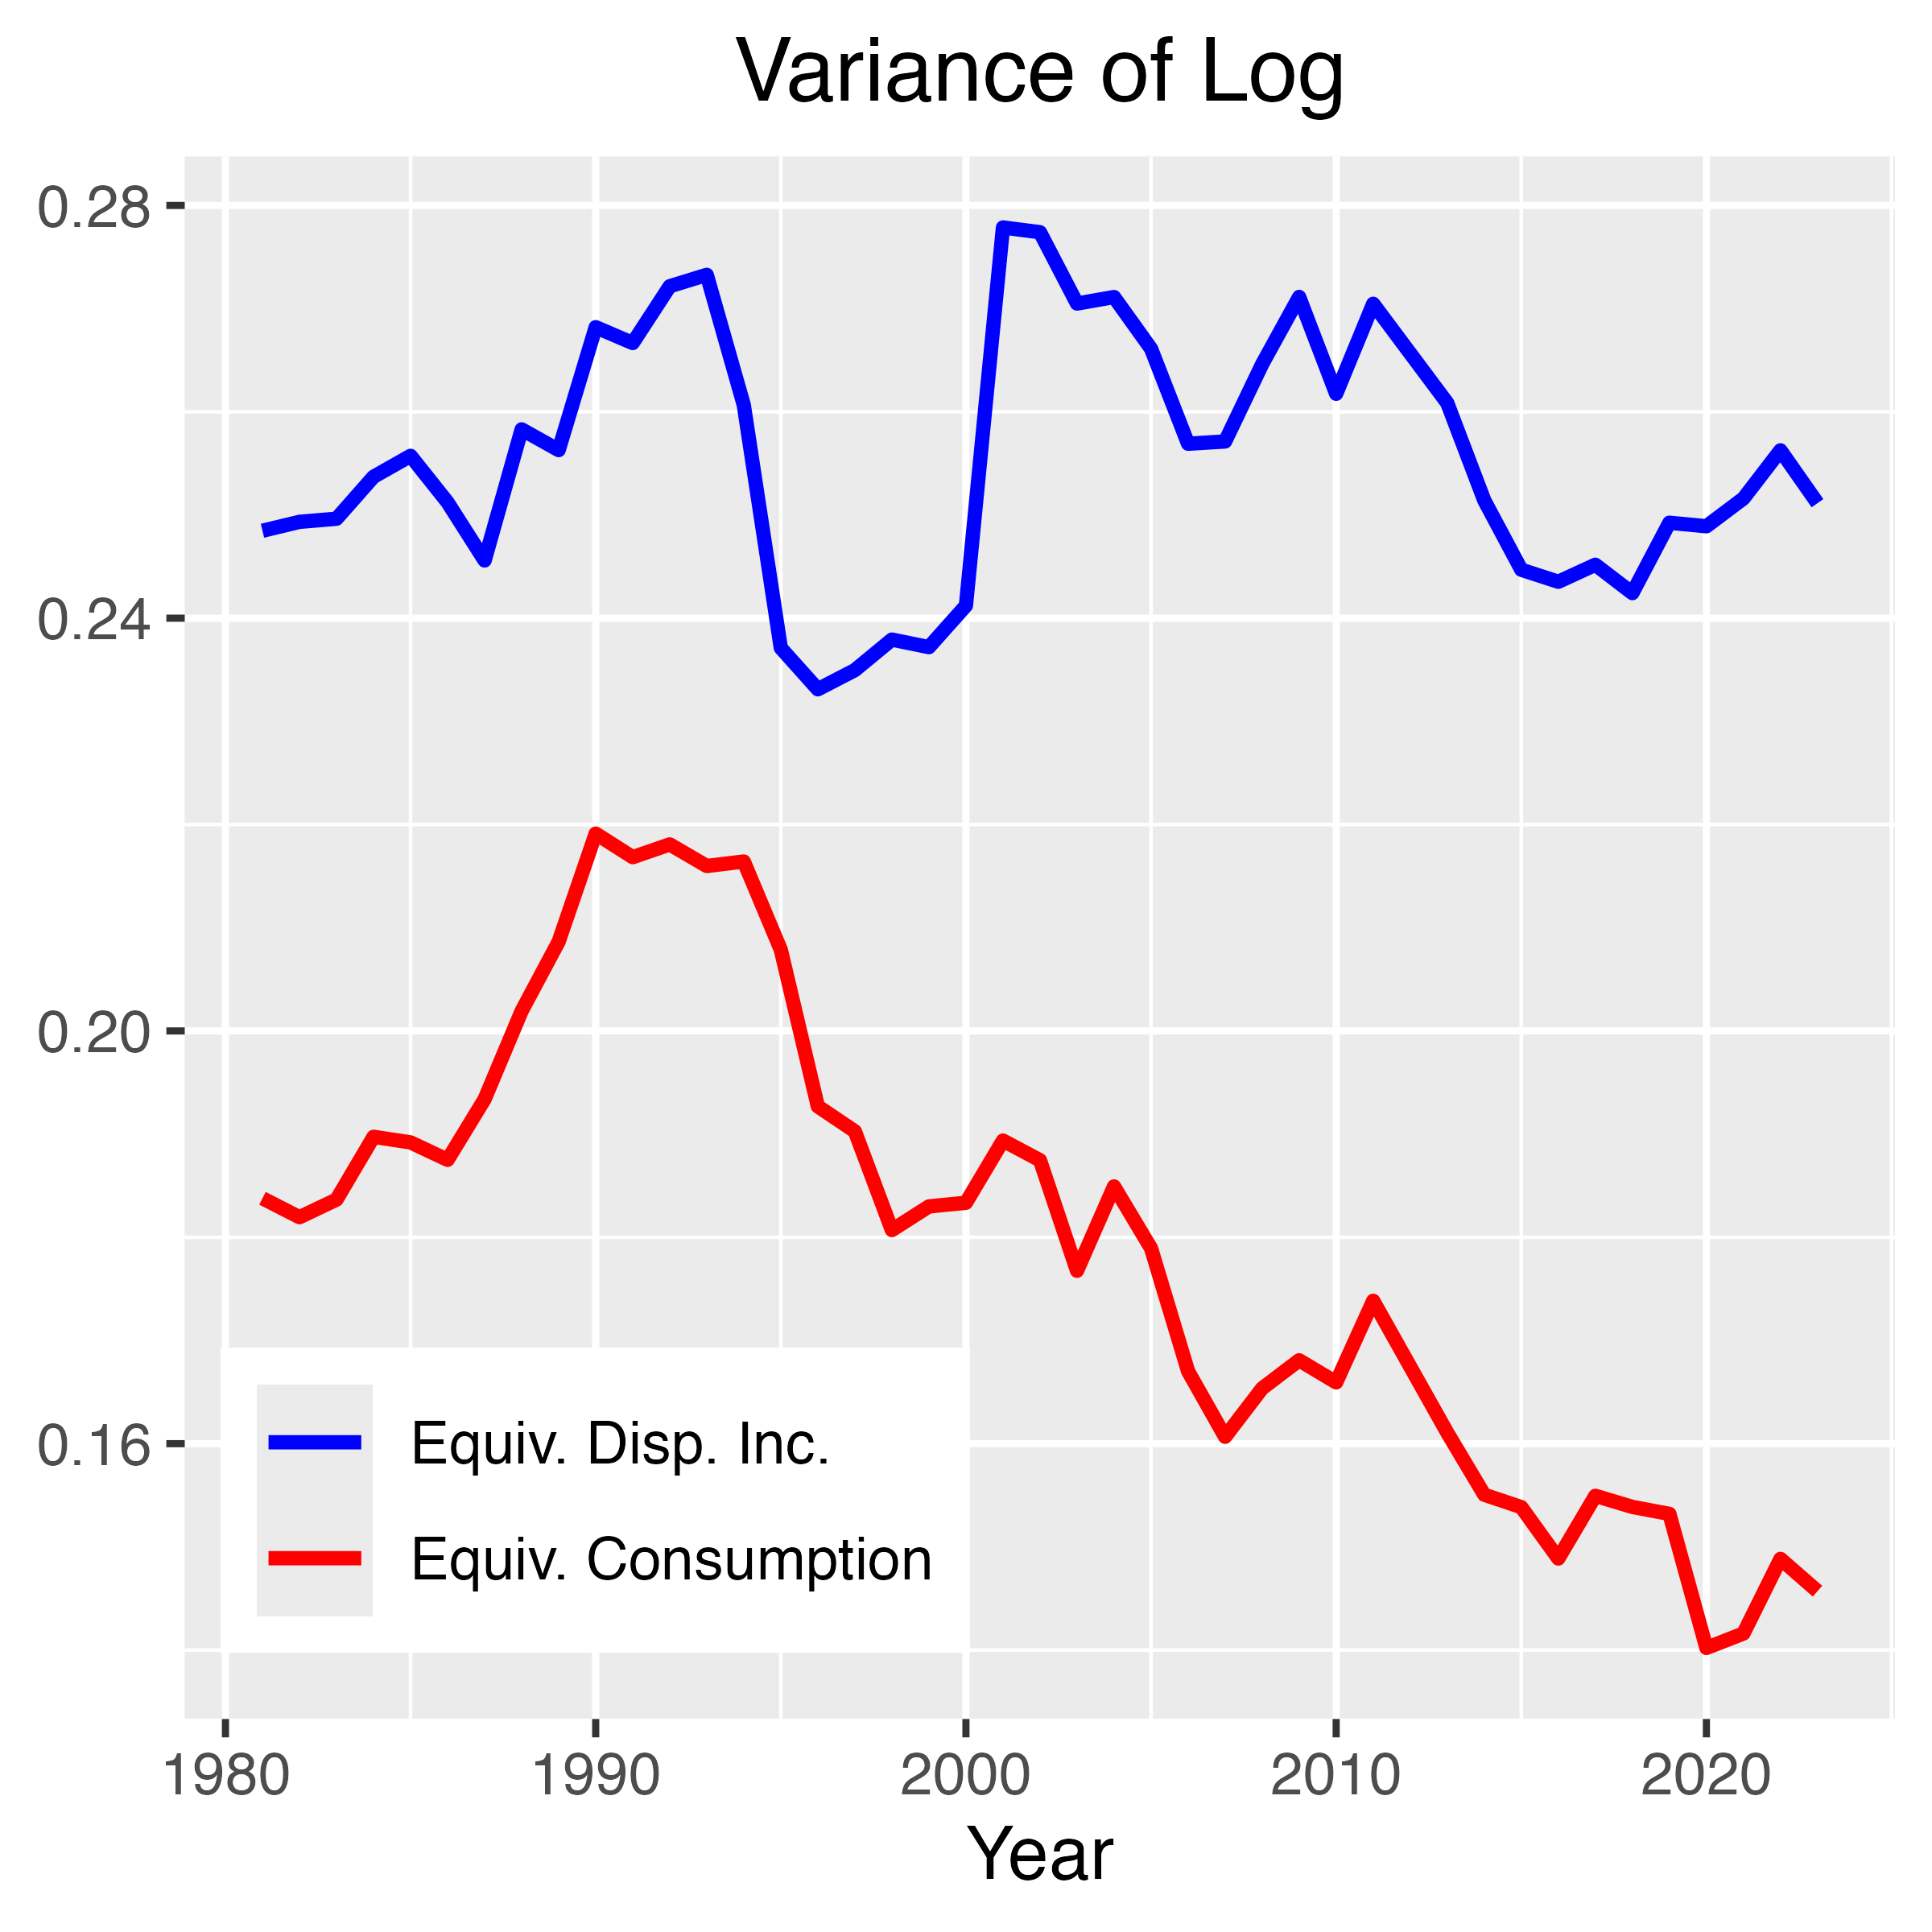
\includegraphics[width=\textwidth]{figures/Fig_6/Fig_6a.png}
    \end{subfigure}
    \begin{subfigure}[t]{0.475\textwidth}
        \centering
        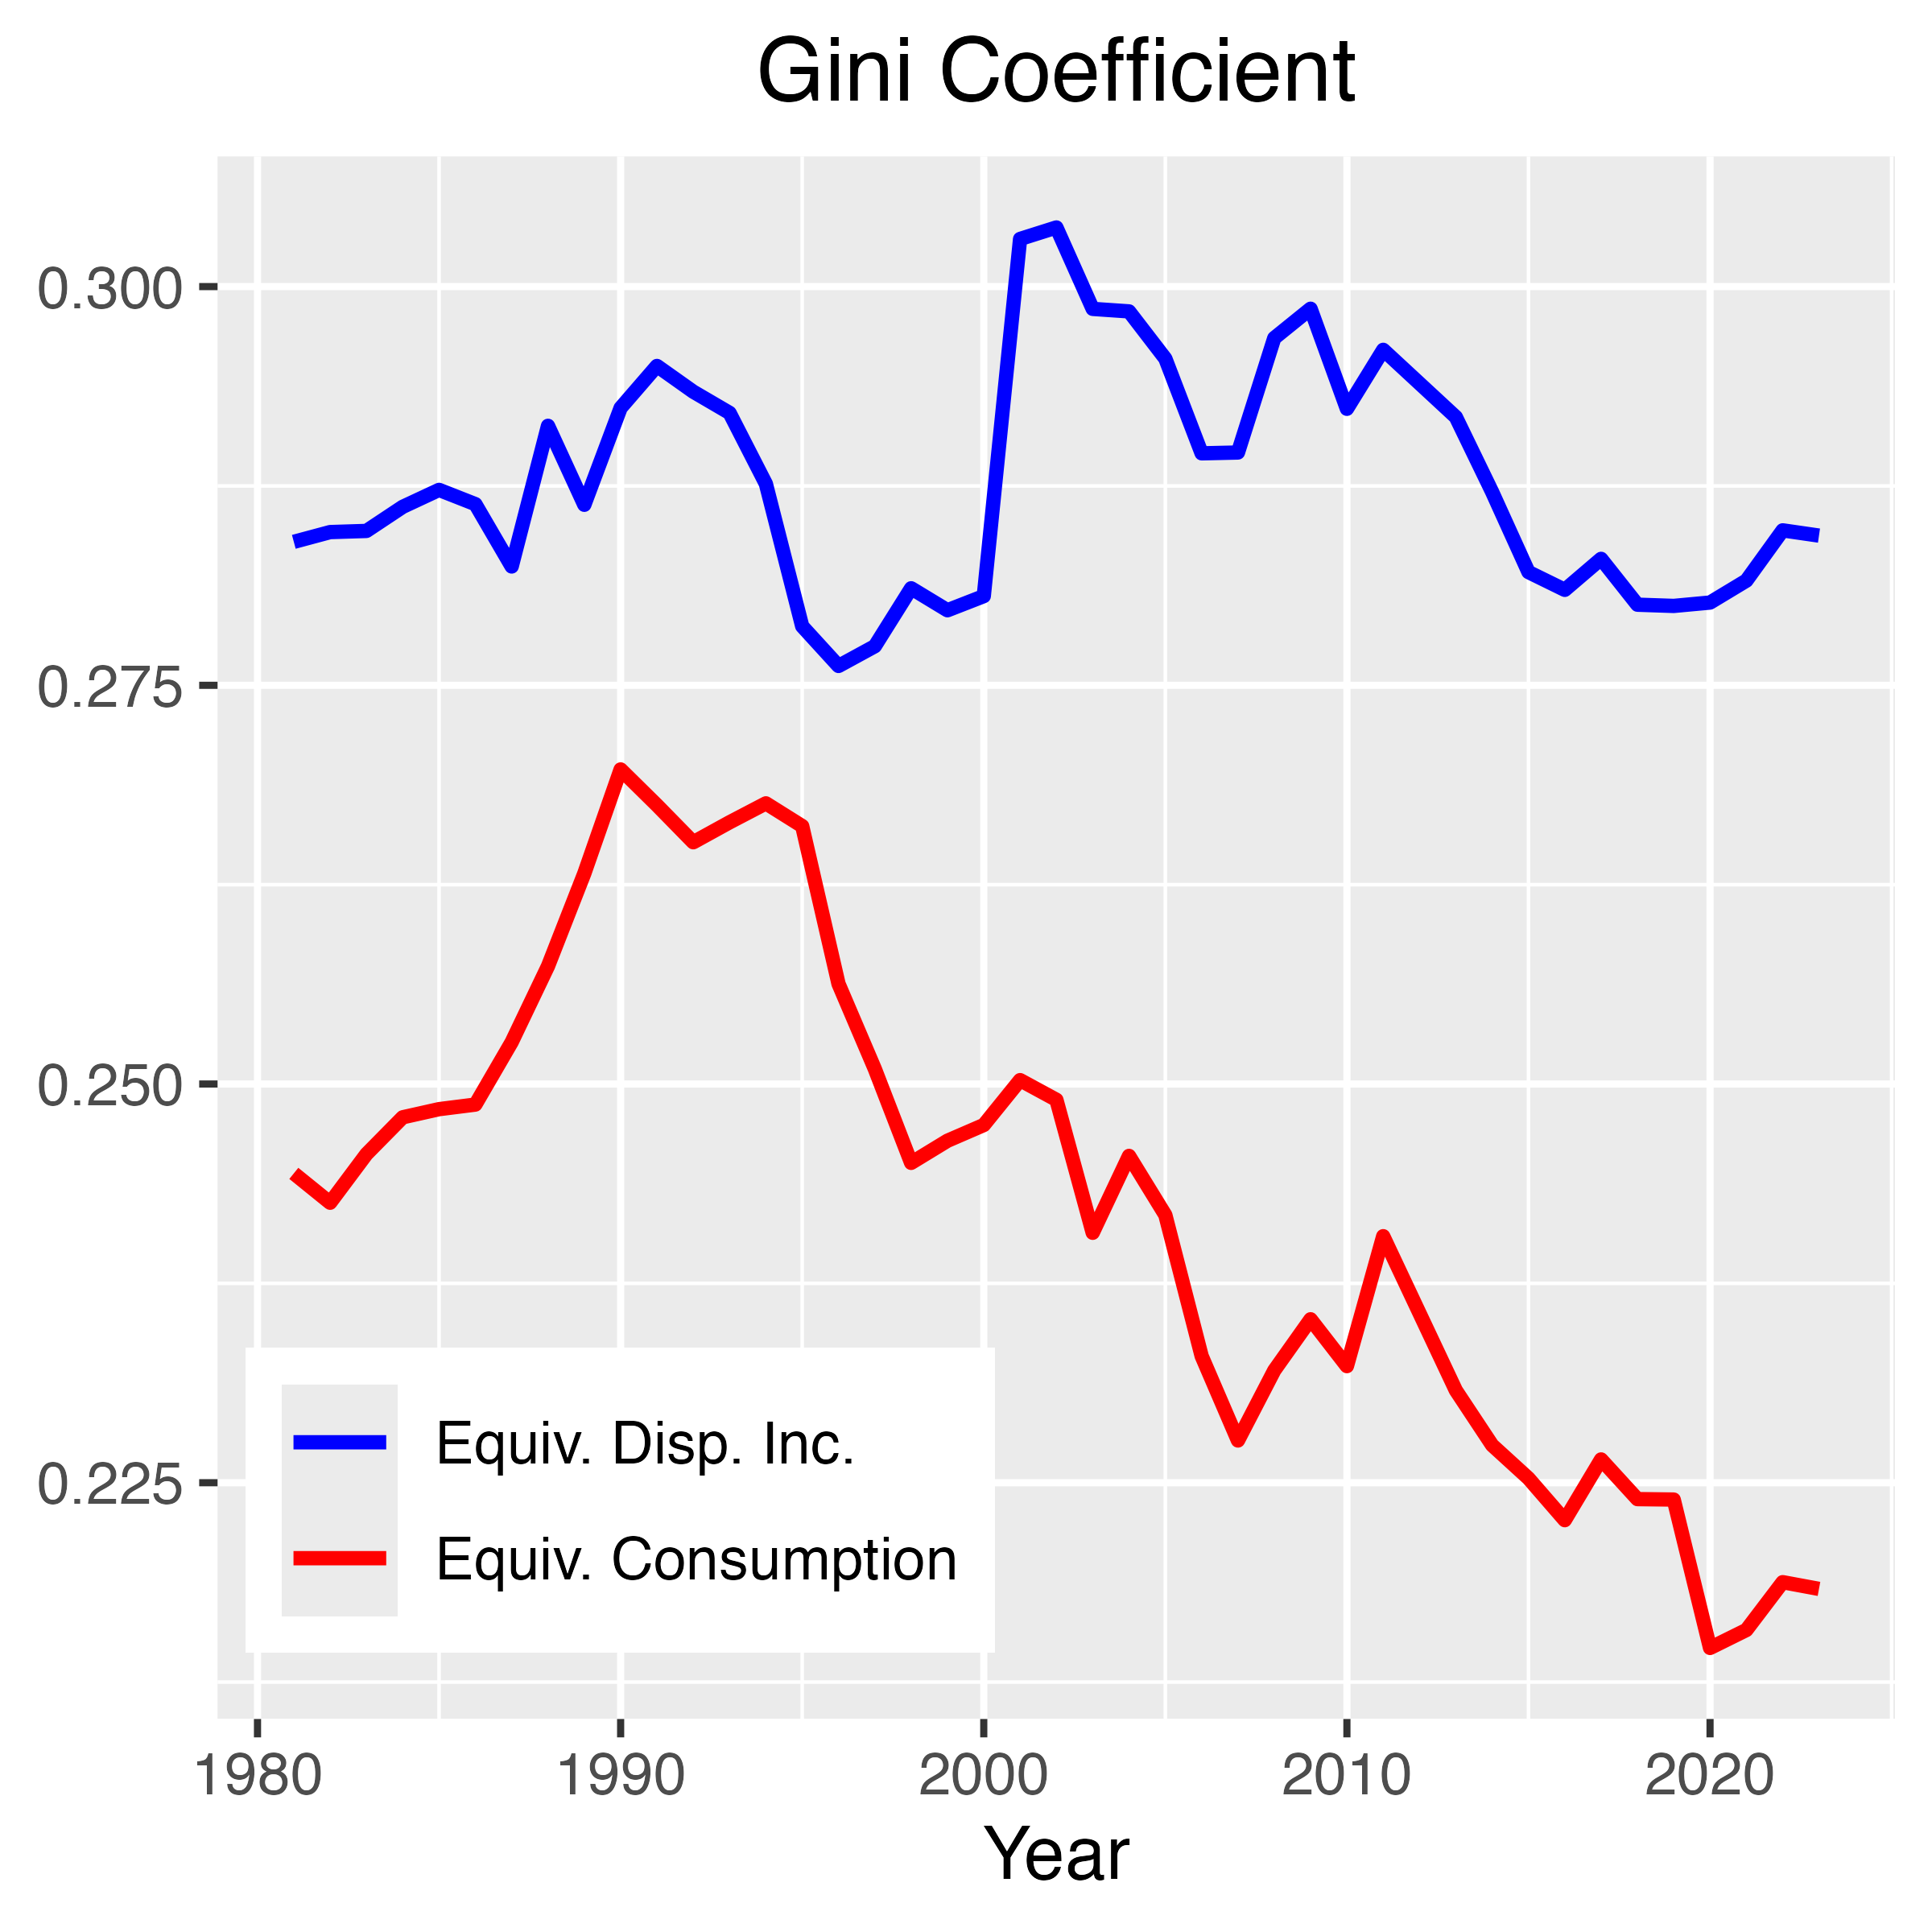
\includegraphics[width=\textwidth]{figures/Fig_6/Fig_6b.png}
    \end{subfigure}
    \begin{subfigure}[t]{0.475\textwidth}
        \centering
        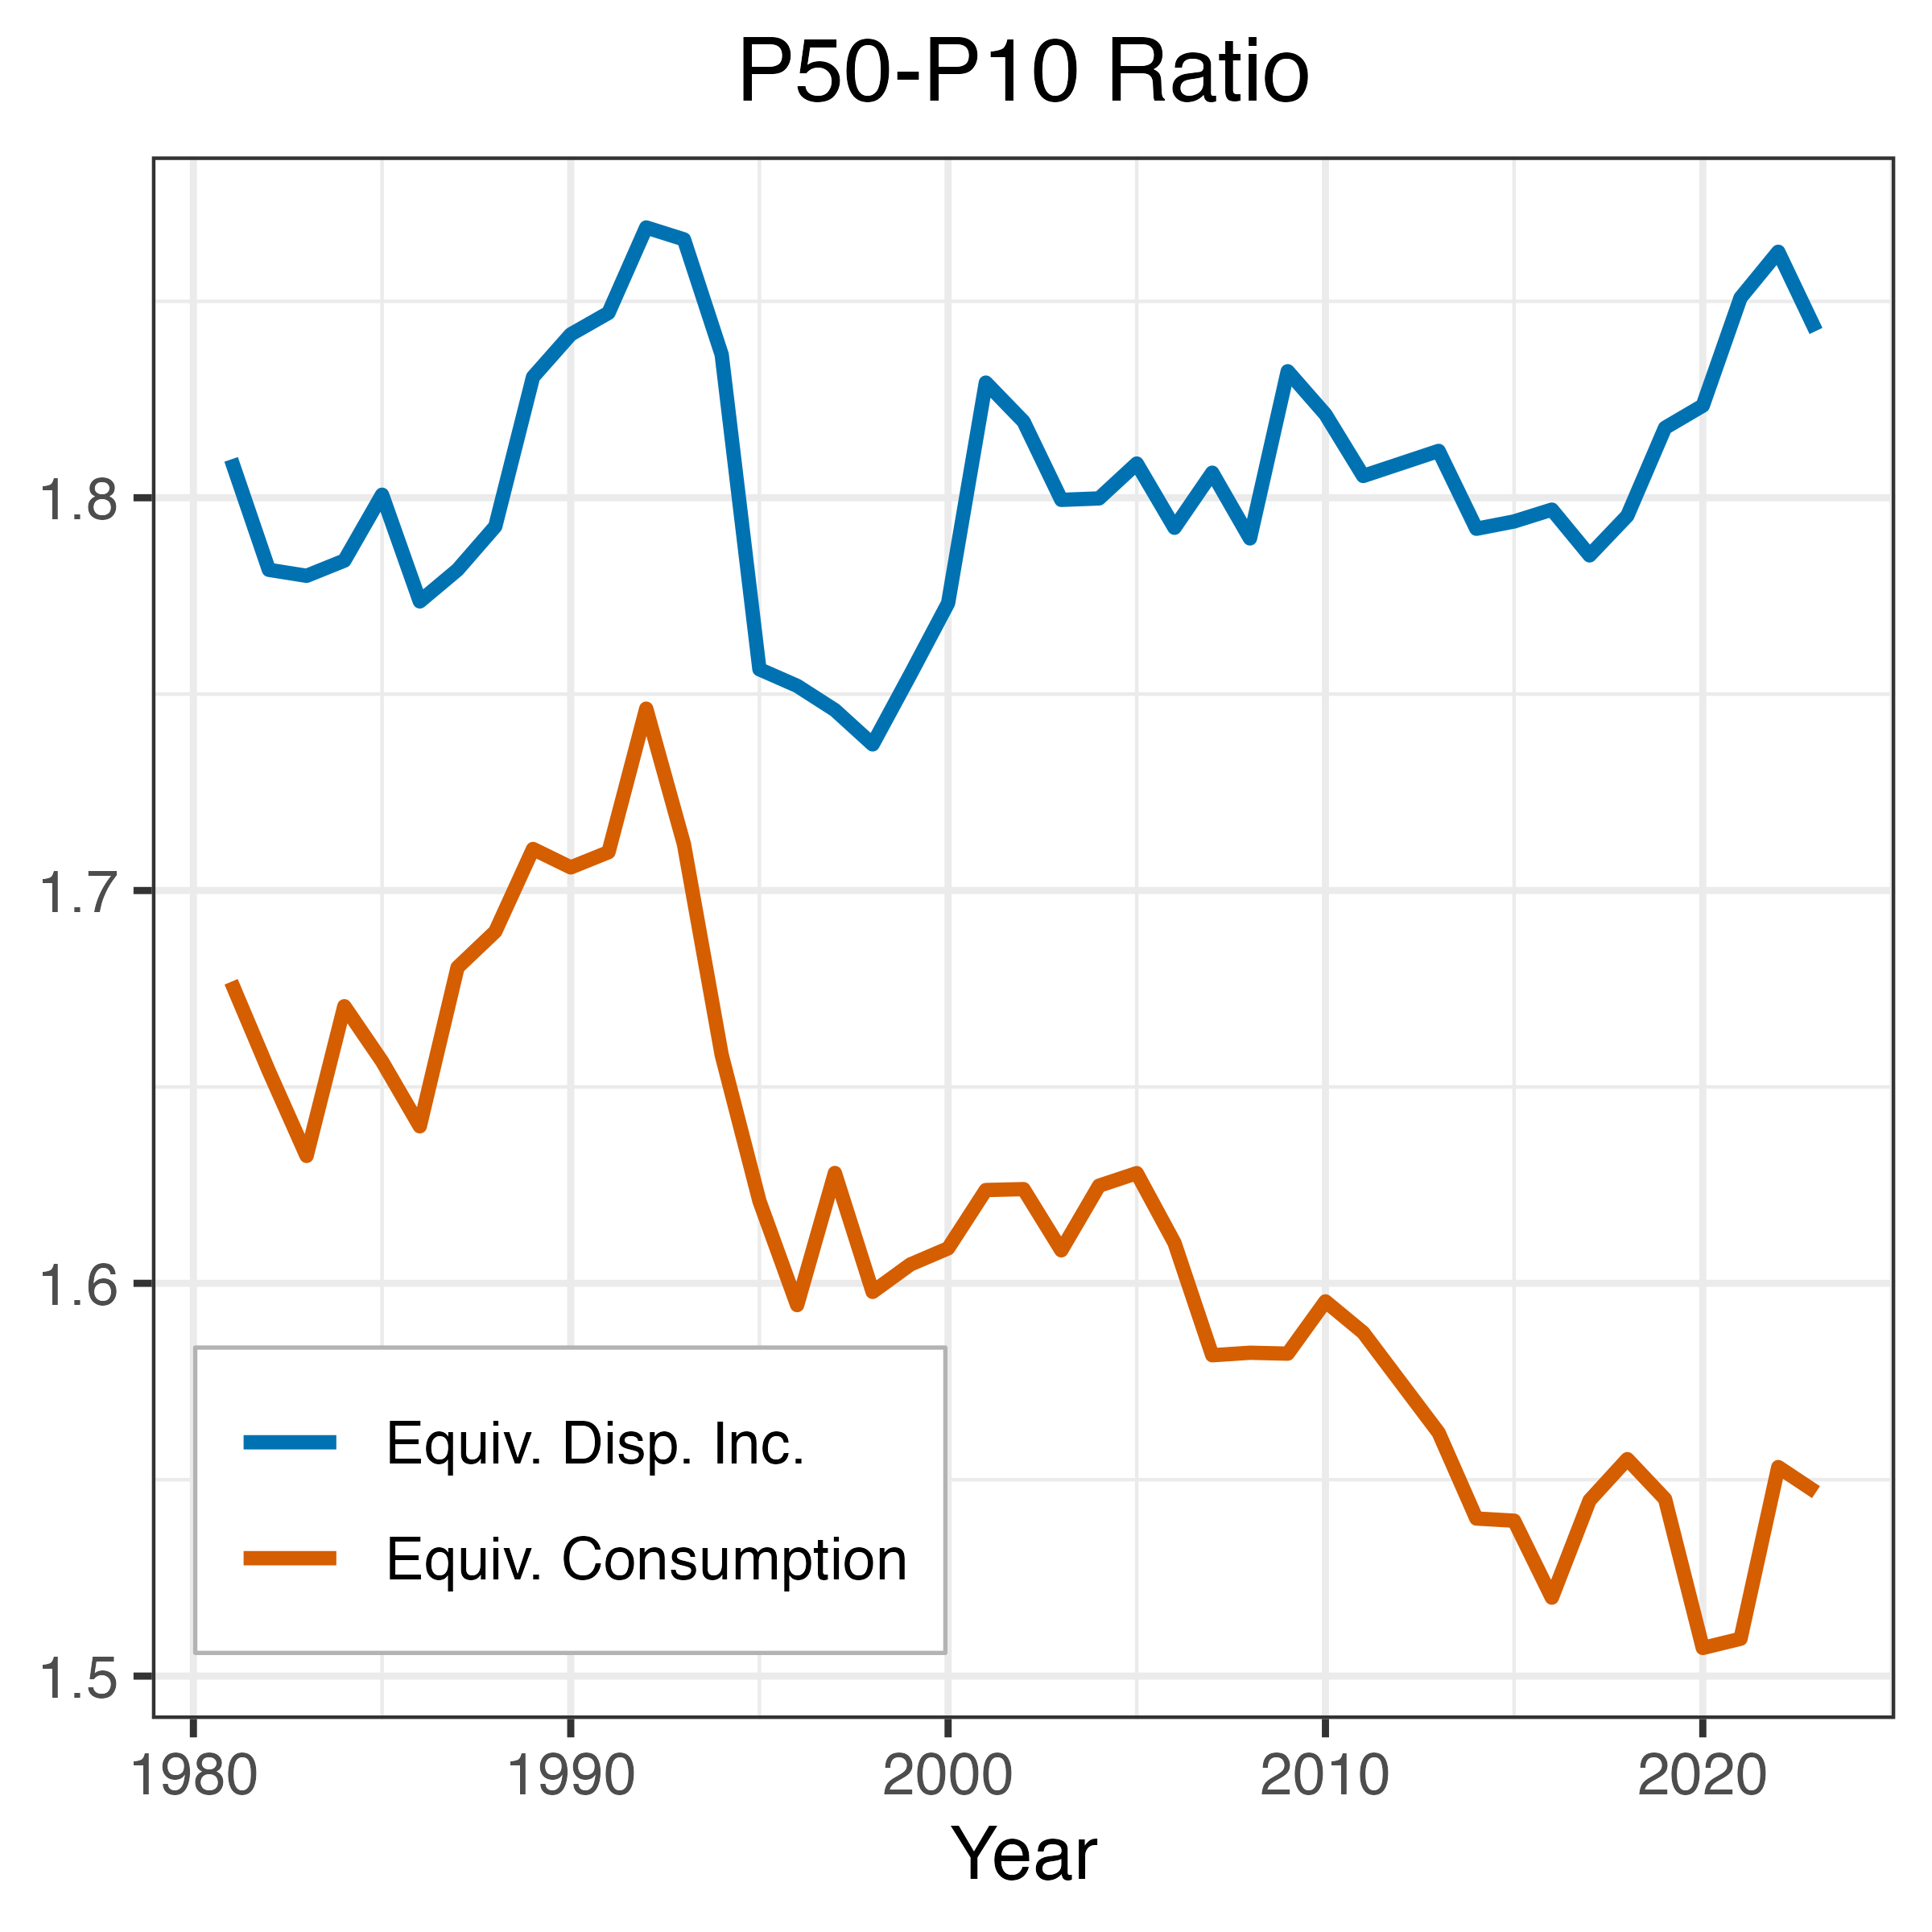
\includegraphics[width=\textwidth]{figures/Fig_6/Fig_6c.png}
    \end{subfigure}
    \begin{subfigure}[t]{0.475\textwidth}
        \centering
        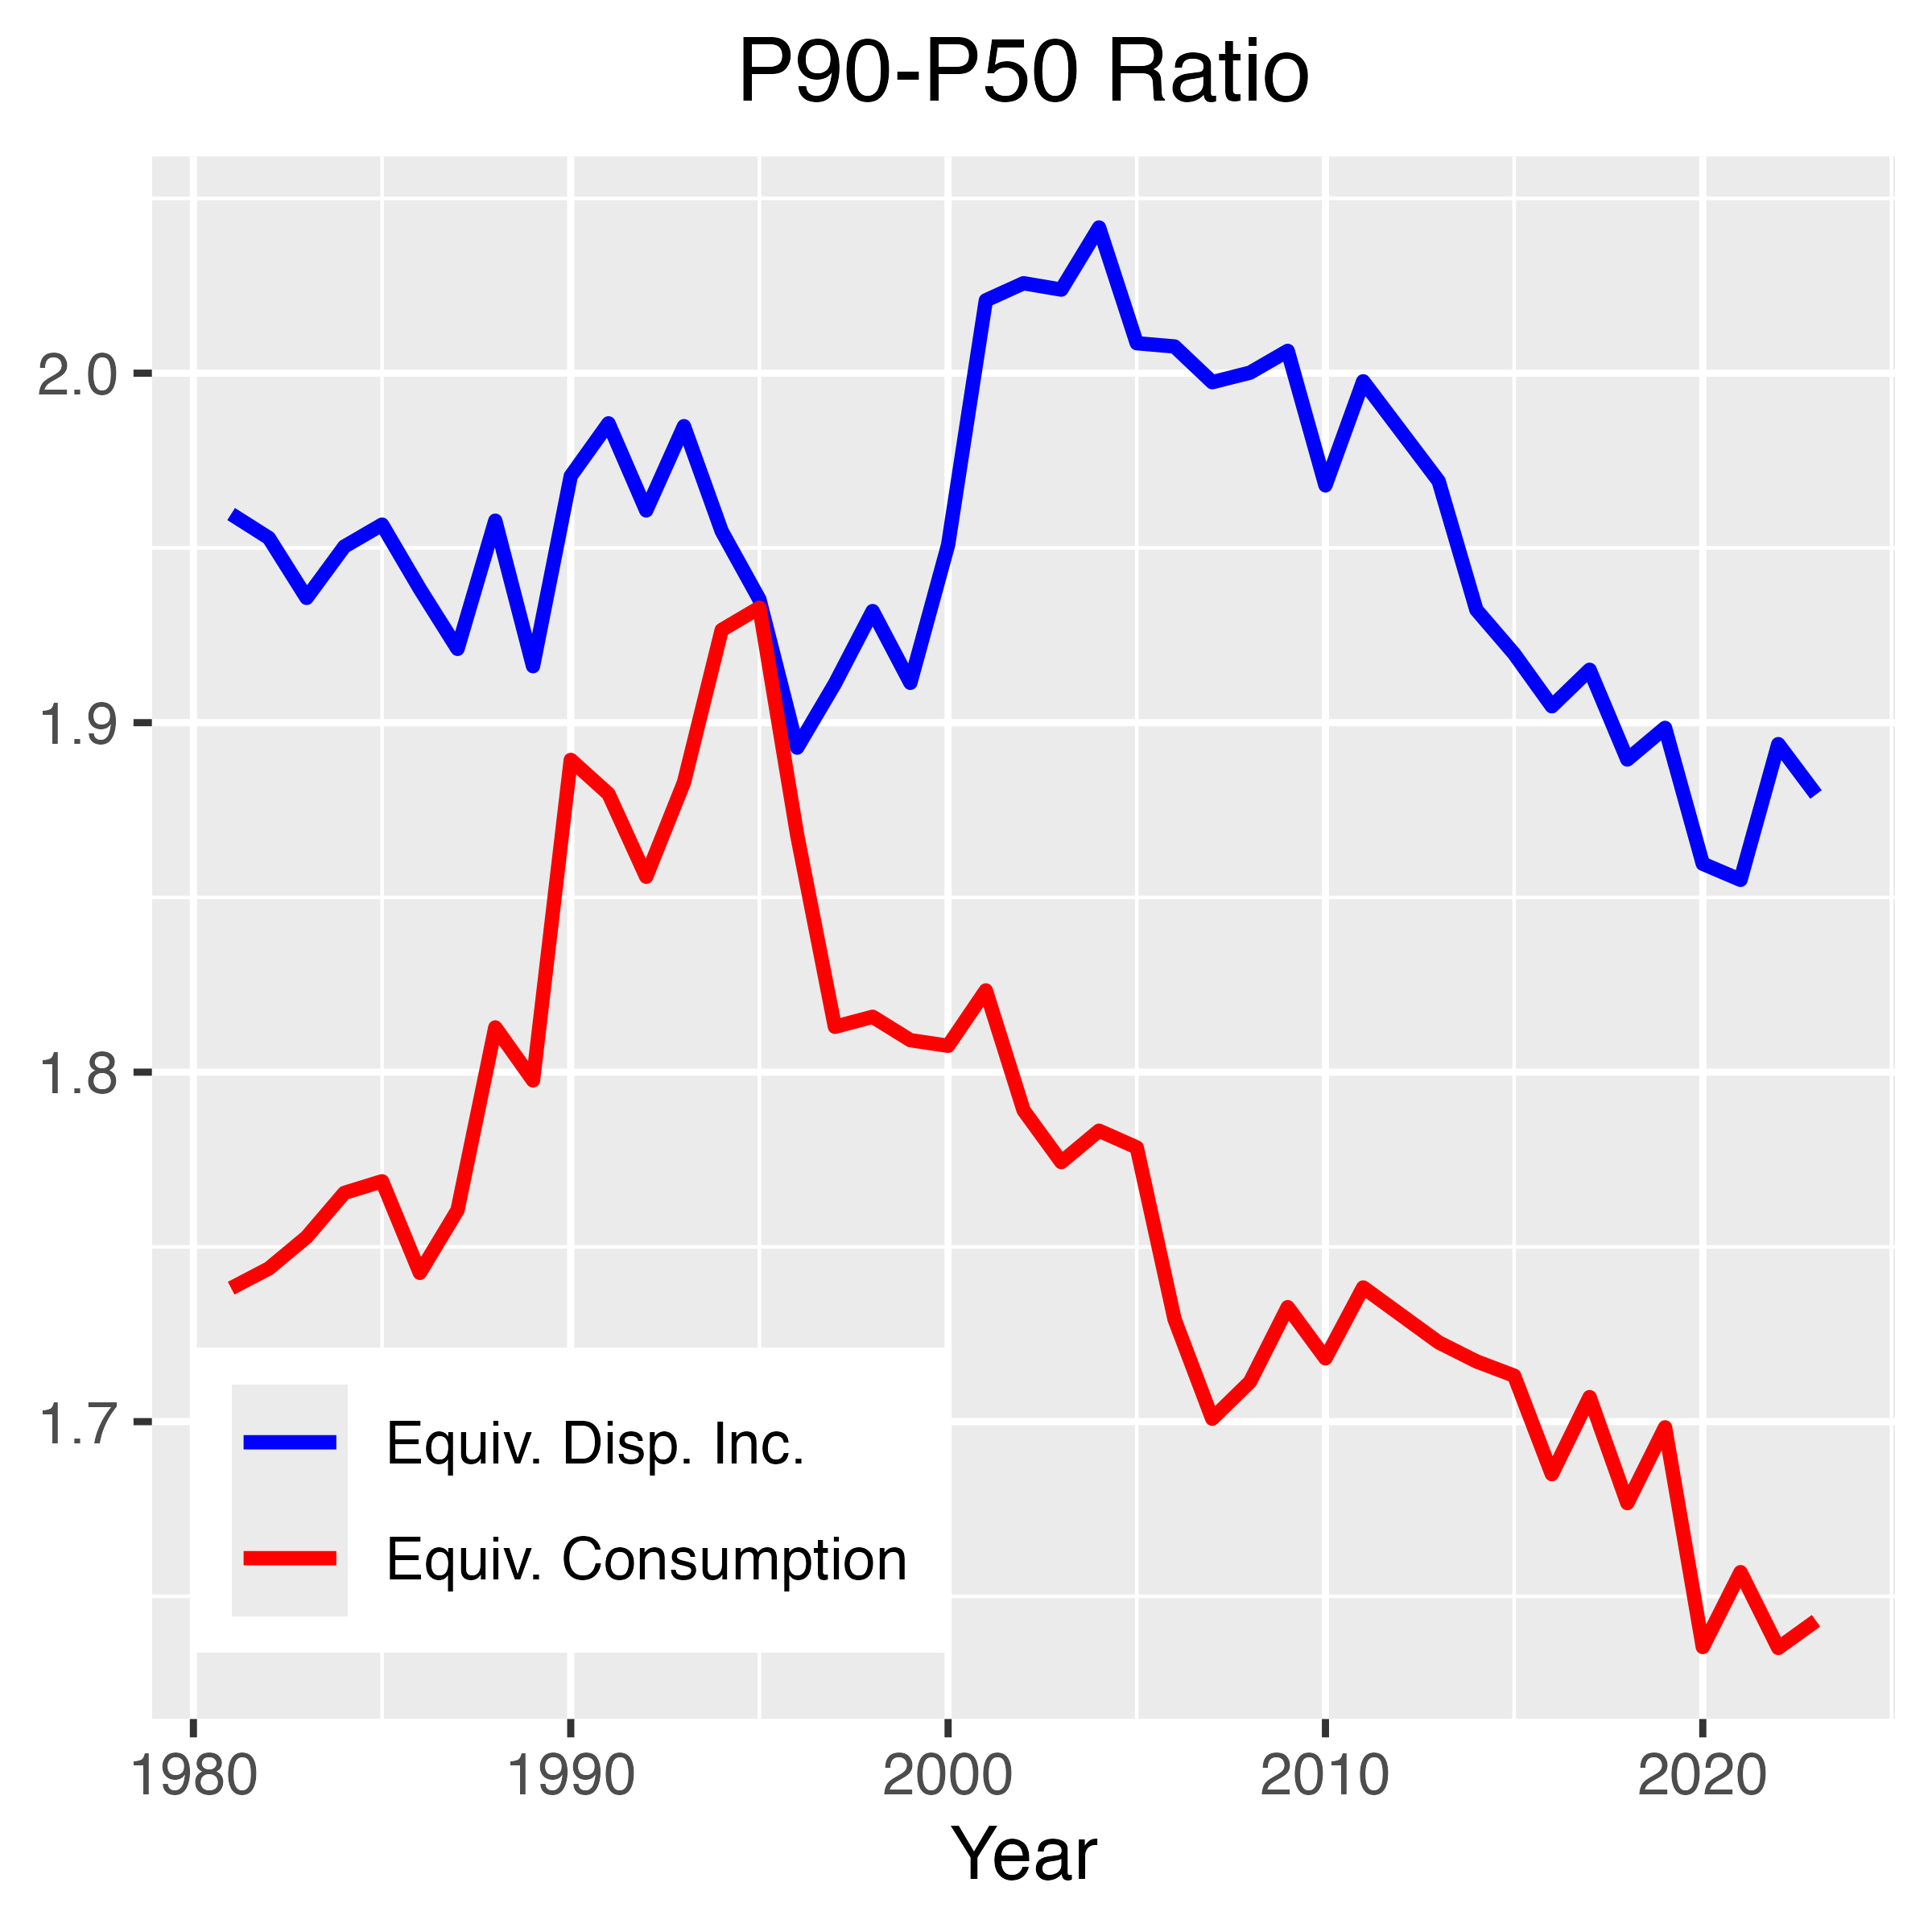
\includegraphics[width=\textwidth]{figures/Fig_6/Fig_6d.png}
    \end{subfigure}
    \caption{From Disposable Income to Consumption}
    \label{fig:Consumption}
\end{figure}

\begin{figure}[htbp]
    \centering
    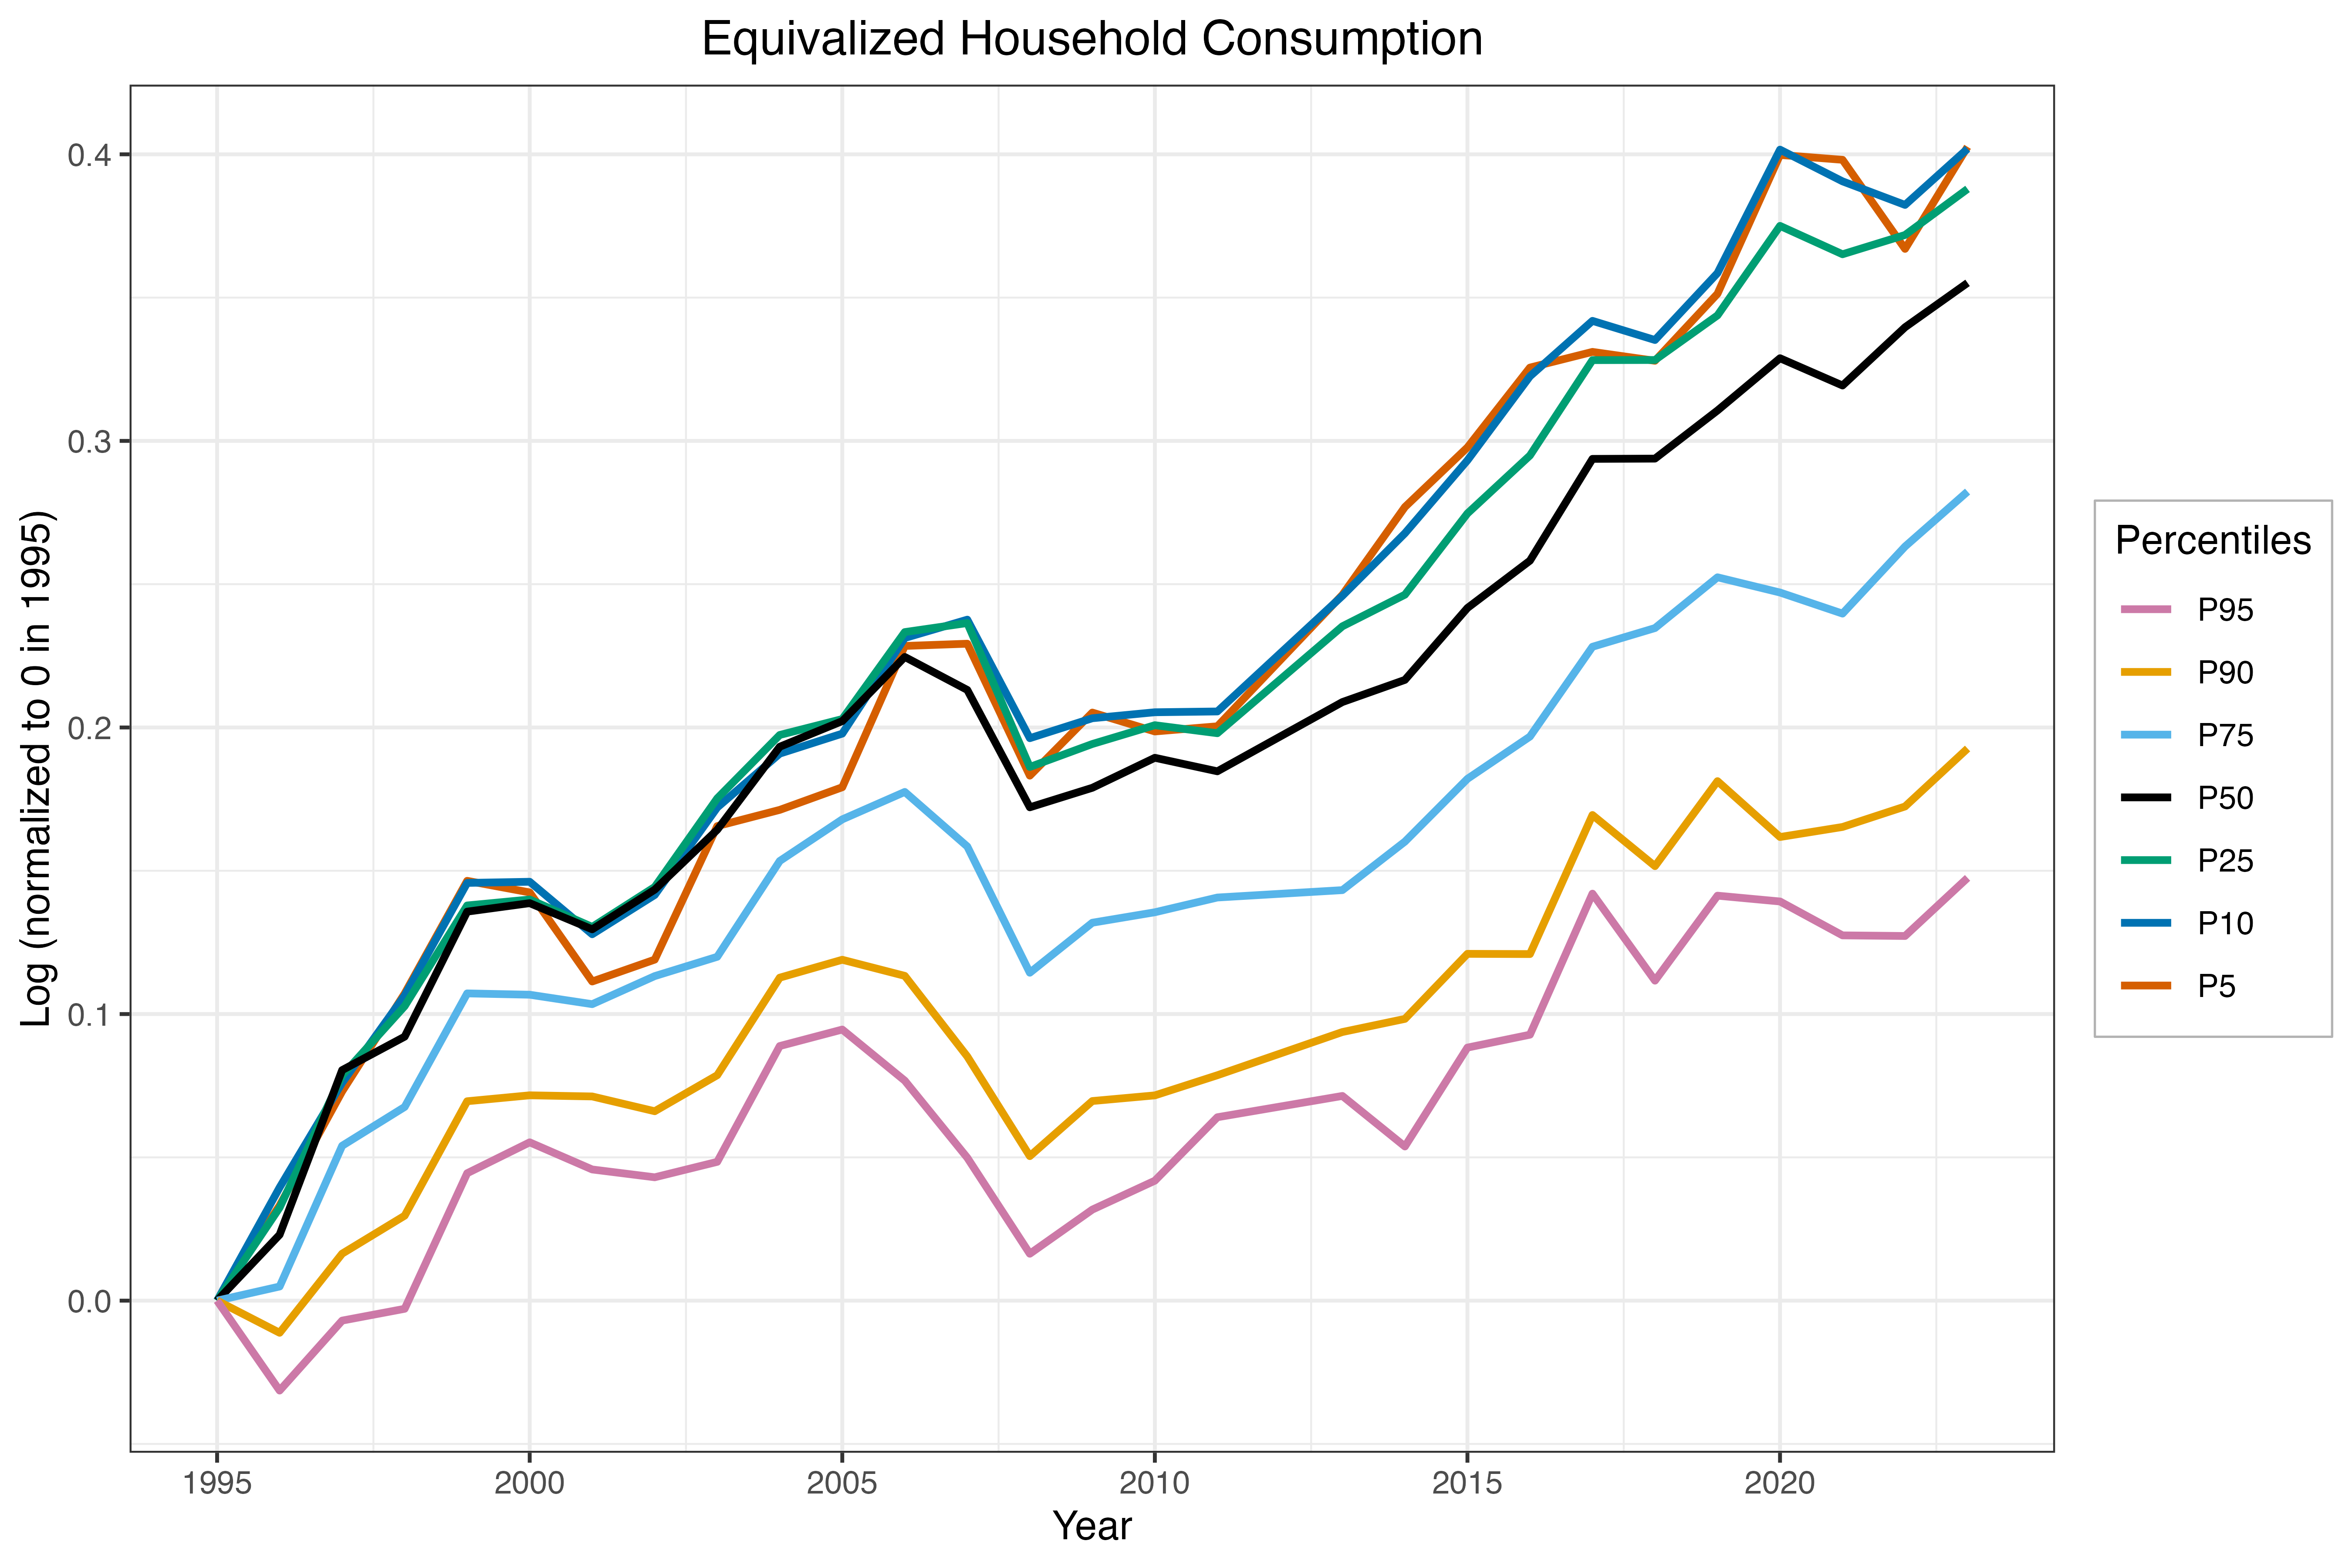
\includegraphics[width=0.95\textwidth]{figures/Fig_7/Fig_7_percentiles_a1995.png}
    \caption{Percentiles of the Household Consumption Distribution}
    \label{fig:Consumption_cyclic}
\end{figure}


\begin{figure}[t]
    \centering
    \begin{subfigure}[t]{0.475\textwidth}
        \centering
        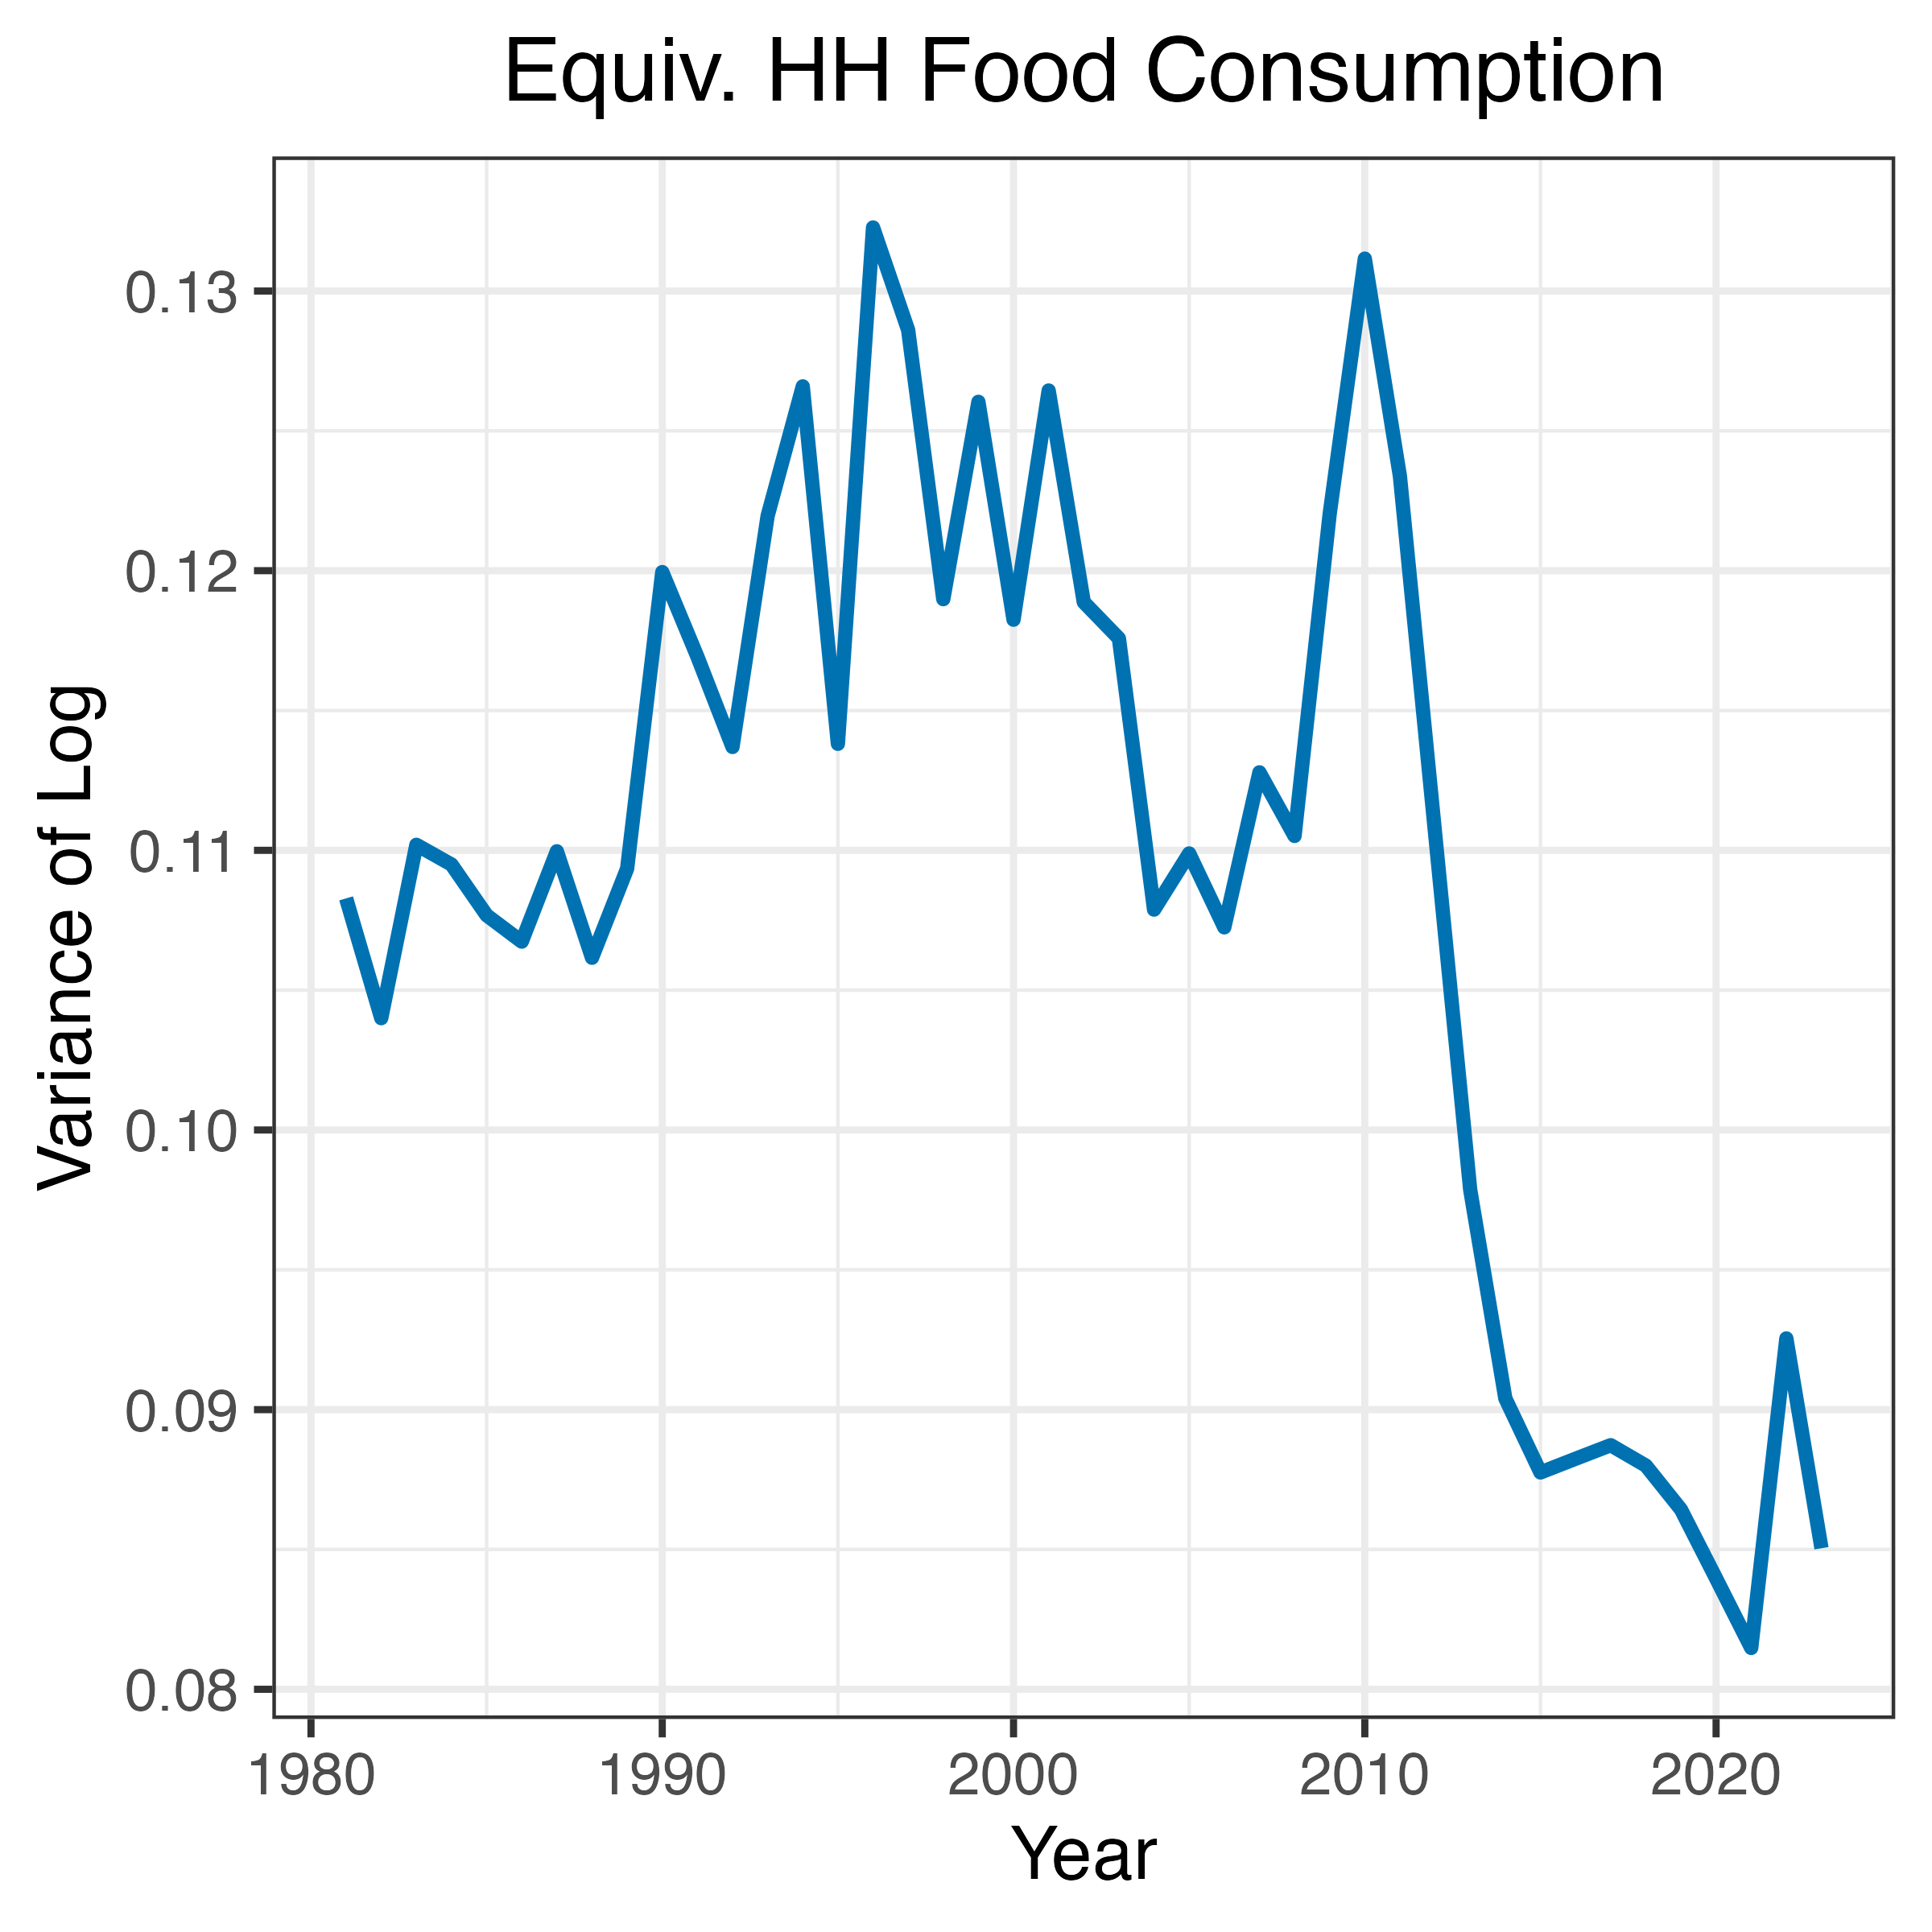
\includegraphics[width=\textwidth]{figures/Fig_8/Fig_8a_Var_Food.png}
    \end{subfigure}
    \begin{subfigure}[t]{0.475\textwidth}
        \centering
        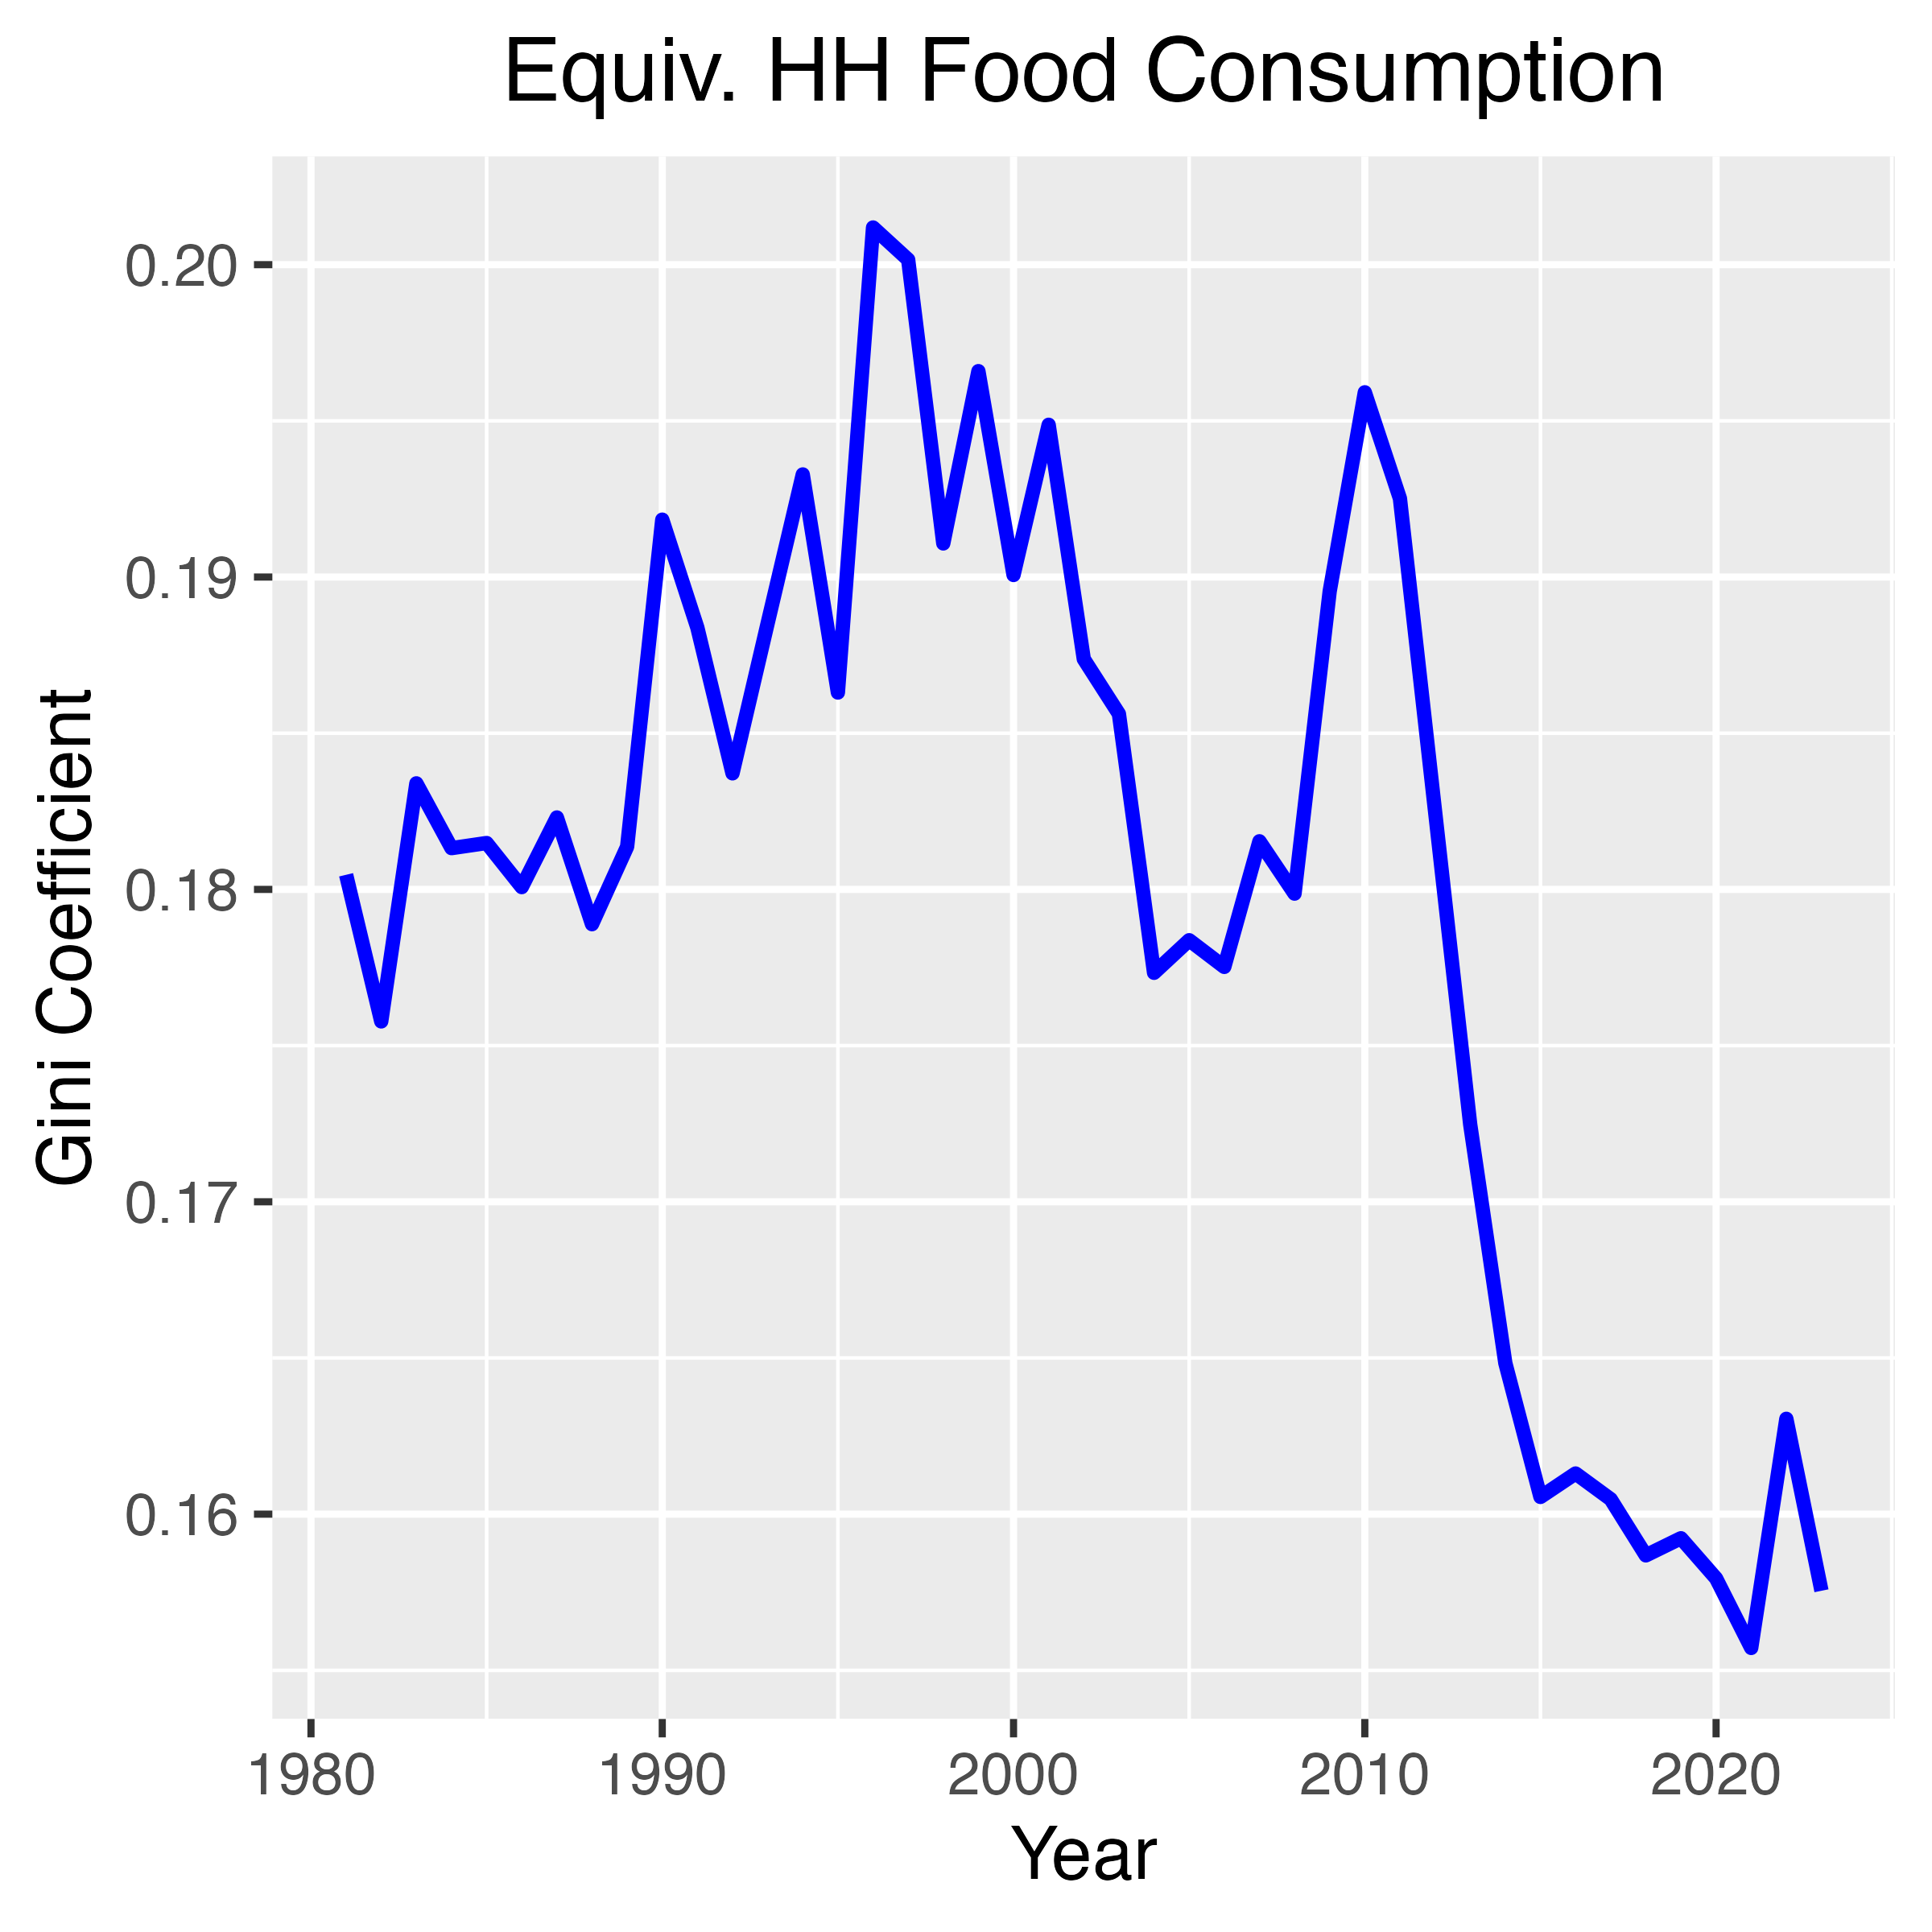
\includegraphics[width=\textwidth]{figures/Fig_8/Fig_8b_Gini_Food.png}
    \end{subfigure}
    \begin{subfigure}[t]{0.475\textwidth}
        \centering
        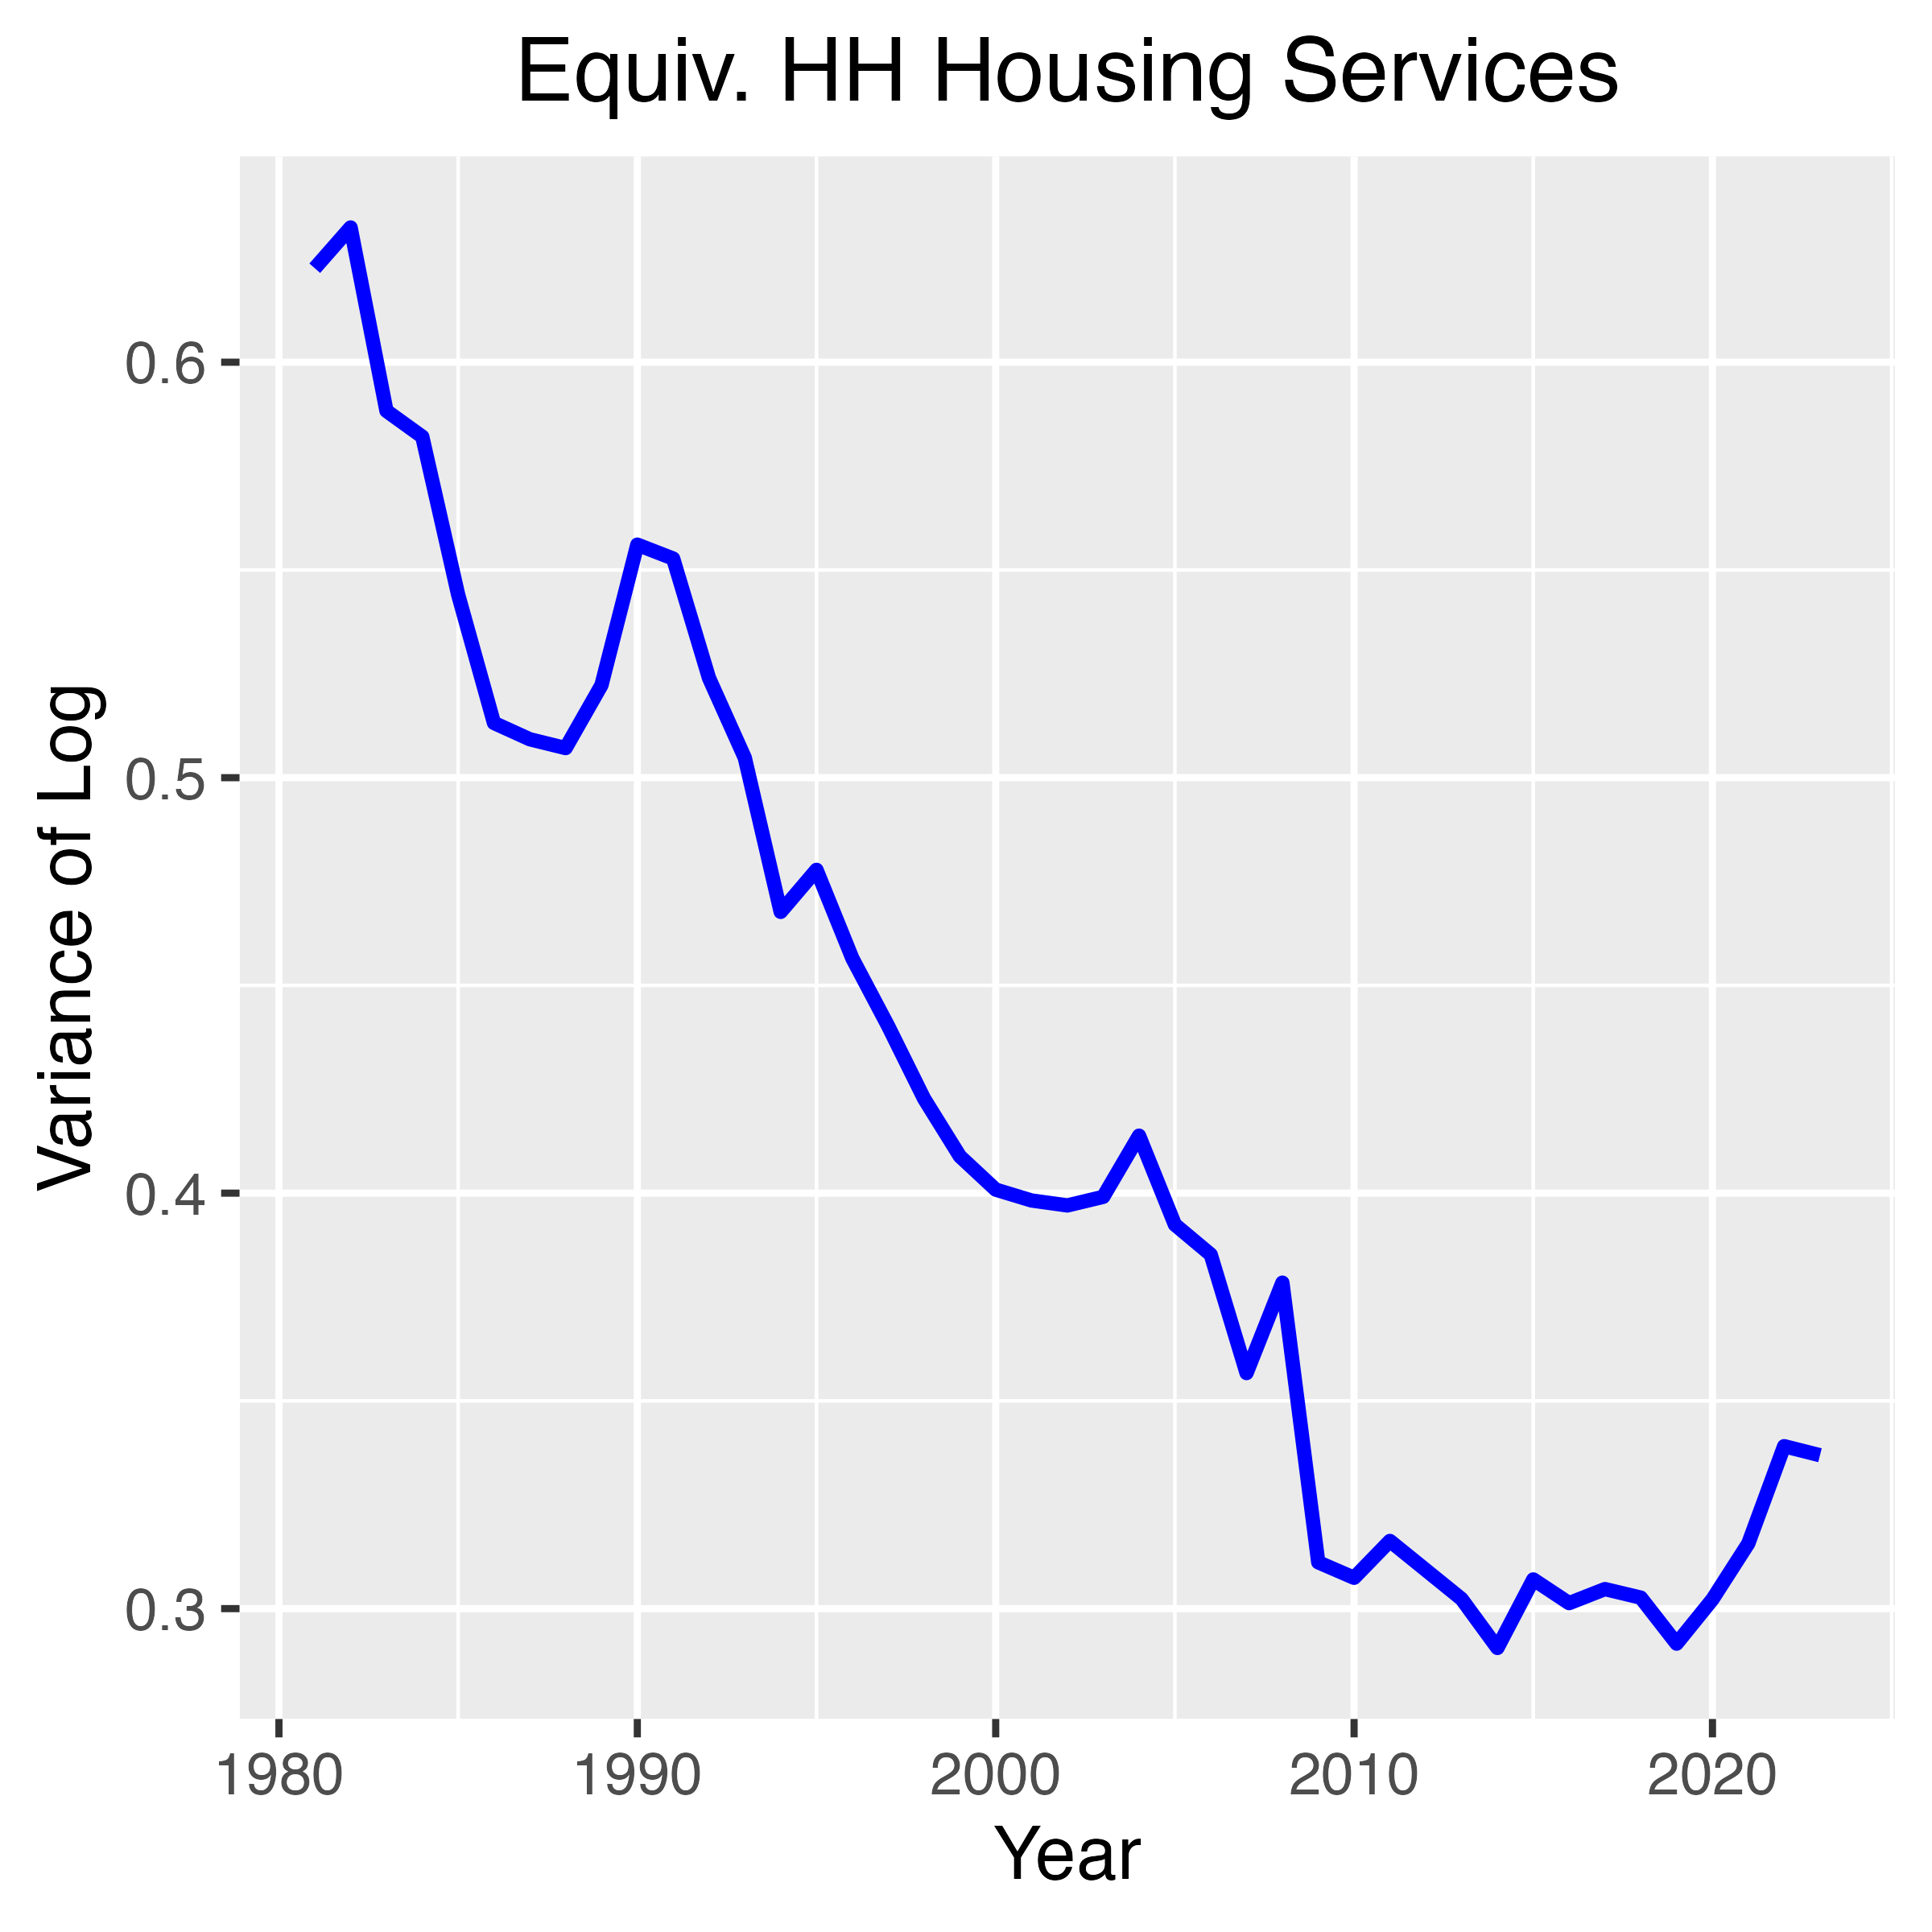
\includegraphics[width=\textwidth]{figures/Fig_8/Fig_8c_Var_Housing.png}
    \end{subfigure}
    \begin{subfigure}[t]{0.475\textwidth}
        \centering
        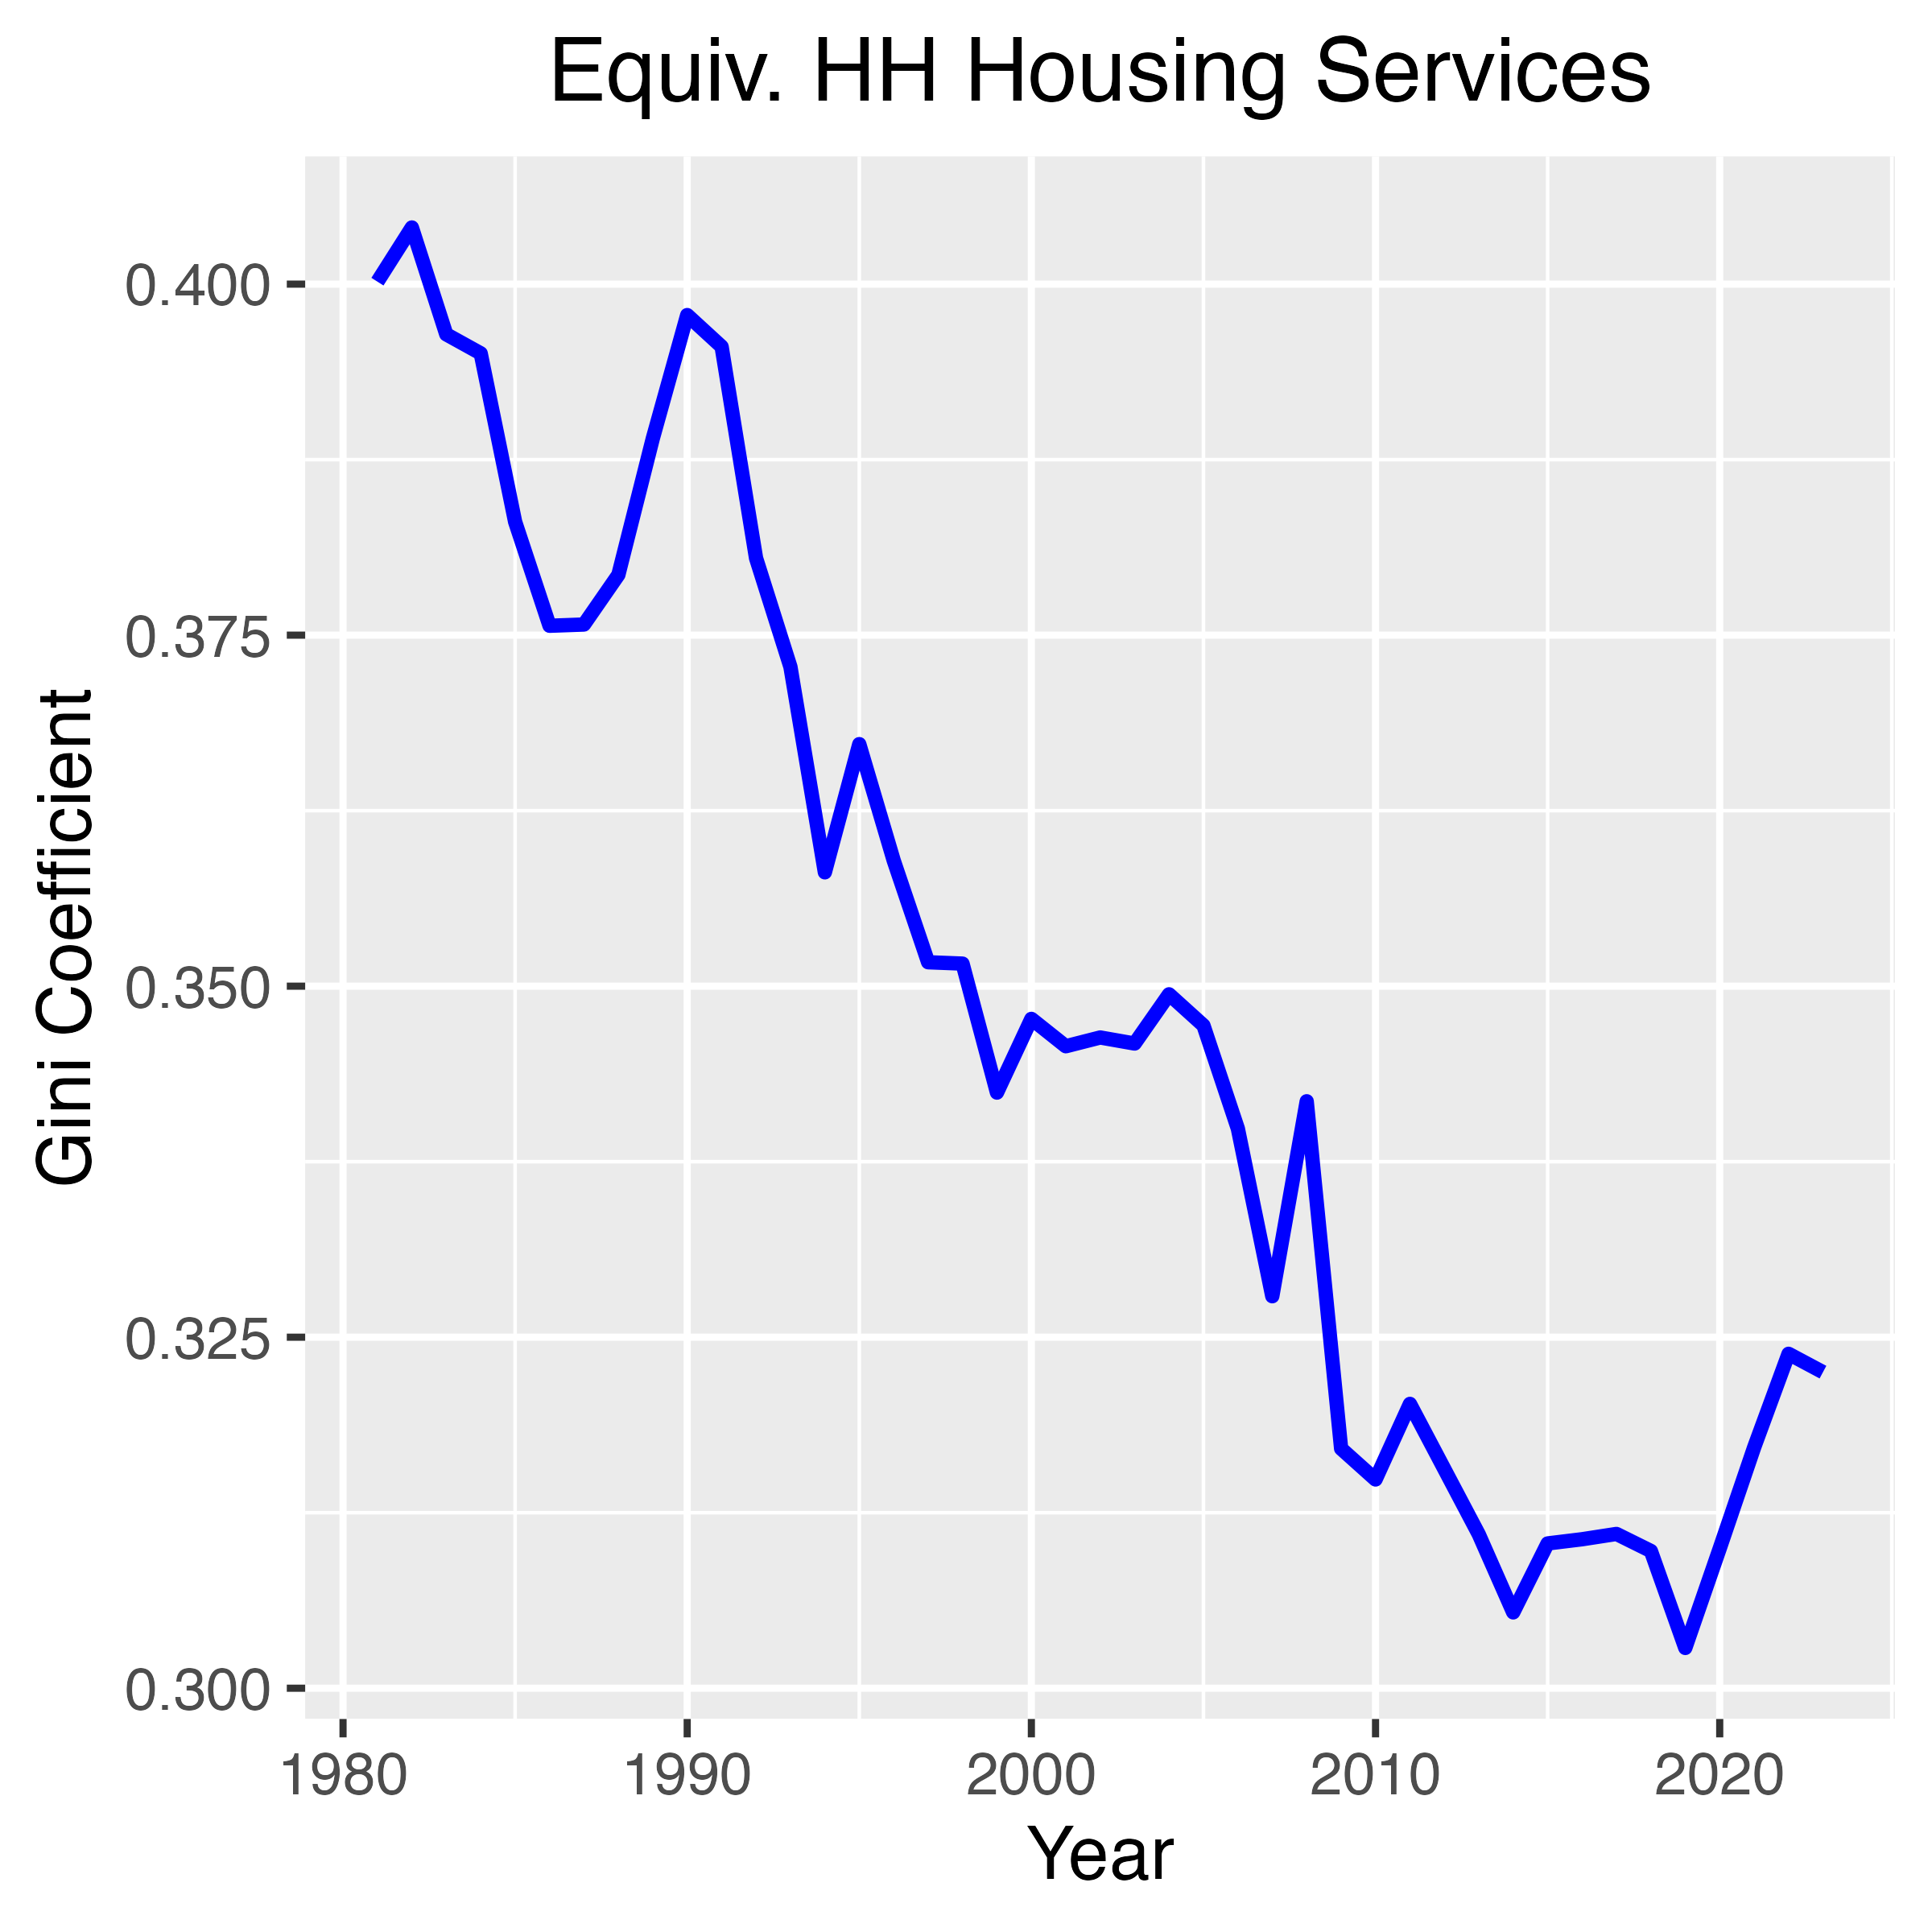
\includegraphics[width=\textwidth]{figures/Fig_8/Fig_8d_Gini_Housing.png}
    \end{subfigure}
    \caption{Food and Housing Consumption Inequality}
    \label{fig:Food_Housing}
\end{figure}

\subsection{Government Redistribution}

We move on to government redistribution in Figure \ref{fig:Gov}. Redistribution plays a significant role in reducing income inequality. We can see that although both benefits and taxes reduce inequality, welfare systems such as public health insurance and labor insurance have a more substantial redistribution effect. The benefits reduce the Gini coefficient by about 3 points in recent years, and tax further reduces it by 0.6 points, resulting in a much smoother trend.

Compared with the rising variance and Gini coefficient of pre-government income, redistribution successfully stabilized income inequality, making the Gini coefficient stable around 0.29. However, the government did not smooth out the sharp increases in inequality during recessions such as the Dot-com bubble in 2000 and the Global Financial Crisis in 2008. Surprisingly, COVID-19 did not increase inequality significantly after 2020. This may be due to government subsidies and spending, which stabilized the disparity at the time.

\subsection{From Income to Consumption Inequality}

The rest of this section discusses consumption and expenditure. Figure \ref{fig:Consumption} shows the same four measures as Figure \ref{fig:earnings_inequality} for disposable income and consumption. The result highlights the effect of consumption smoothing. Since households can borrow and save to maintain consumption when facing income shocks, consumption inequality is smaller than income inequality.

Surprisingly, compared with the US, where consumption inequality increased (Attanasio \& Pistaferri, \citeyear{JEP_Consumption_Inequality}), consumption discrepancies in Taiwan decreased steadily after 1995. One of the reasons could be the low consumption growth rate of wealthy families, as shown in Figure \ref{fig:Consumption_cyclic}. The full series from 1981 are in Appendix Figures \ref{fig:appendix_cyclic_consumption_1981} and \ref{fig:appendix_cyclic_consumption_1995}, normalized to 1981 and 1995 respectively. The consumption expenditures of the top 5\% of families grew by about 15 log points between 1995 and 2023, compared with 39 log points for the lowest 25\%. 

These consumption phenomena could negatively impact Taiwan's economy, as Hong (\citeyear{TW_consumption_inequality}) suggests, since wealthy families do not increase their consumption and lower-income families face higher housing and medical costs. Eventually, this could lead to a stagnation of Taiwan's economy.

\subsection{Food Consumption and Housing Services}

Finally, Figure \ref{fig:Food_Housing} shows inequality in food and housing consumption in Taiwan. The Gini coefficients and variances presented in the figure indicate that the food expenditure discrepancies remain relatively small, and housing consumption inequality is steadily decreasing.

The decrease in food consumption inequality after 2010 is not explained here. A definition change in the survey cannot be ruled out. The food aggregate is built from one set of item codes through 2008, another in 2009, and a third from 2010 onward, so the definition changes just before the decline begins. Separating the two is left for future work.


\section{Conclusion}
\label{sec:conclusion}

This paper provides a comprehensive overview of the long-run evolution of income and consumption inequality in Taiwan from 1981 to 2023 using household-level data from the SFIE. The findings highlight several key trends and shifts over the past four decades. While income inequality has generally increased, consumption inequality has remained relatively stable or declined, indicating the importance of consumption smoothing mechanisms such as saving, borrowing, and intra-family transfers.

The analysis shows that although the variance and Gini coefficient of household earnings have risen, the rise is smaller than in the United States. Over the first 25 years of the sample, the variance of log household earnings increases by 0.16, against roughly 0.30 over a comparable period in the US. Notably, inequality is most pronounced at the bottom of the earnings distribution, where low-income households have gained the least since 1995 and fall the furthest in recessions, most sharply around the Dot-com bubble and the Global Financial Crisis, and more briefly during the COVID-19 pandemic.

Government redistribution through welfare programs and taxation has helped stabilize disposable income inequality, though its effectiveness varies across time and crises. The role of private transfers has also become more significant in mitigating inequality, especially since 2010, emphasizing the extended family's role as a buffer.

Perhaps most intriguingly, the paper documents a declining trend in consumption inequality, driven partly by the low consumption growth of wealthy households and potentially concerning stagnation among higher-income groups. This divergence between income and consumption dynamics underscores the complexity of economic inequality and calls for more policy responses.

While Taiwan's earnings inequality has risen by less than in the United States, shifts in family composition, consumption behavior, and income distribution point to growing vulnerabilities. Further work should investigate the causes behind these demographic and institutional changes and evaluate policies that could promote inclusive growth in an era of slower economic expansion.

\clearpage

\printbibliography

\newpage
% Appendices
\begin{appendices}
\section{Extra Figures for Cyclical Dynamics}
\label{sec:appendix_cyclical_dynamics}

\vspace{2em}

\begin{figure}[ht]
    \centering
    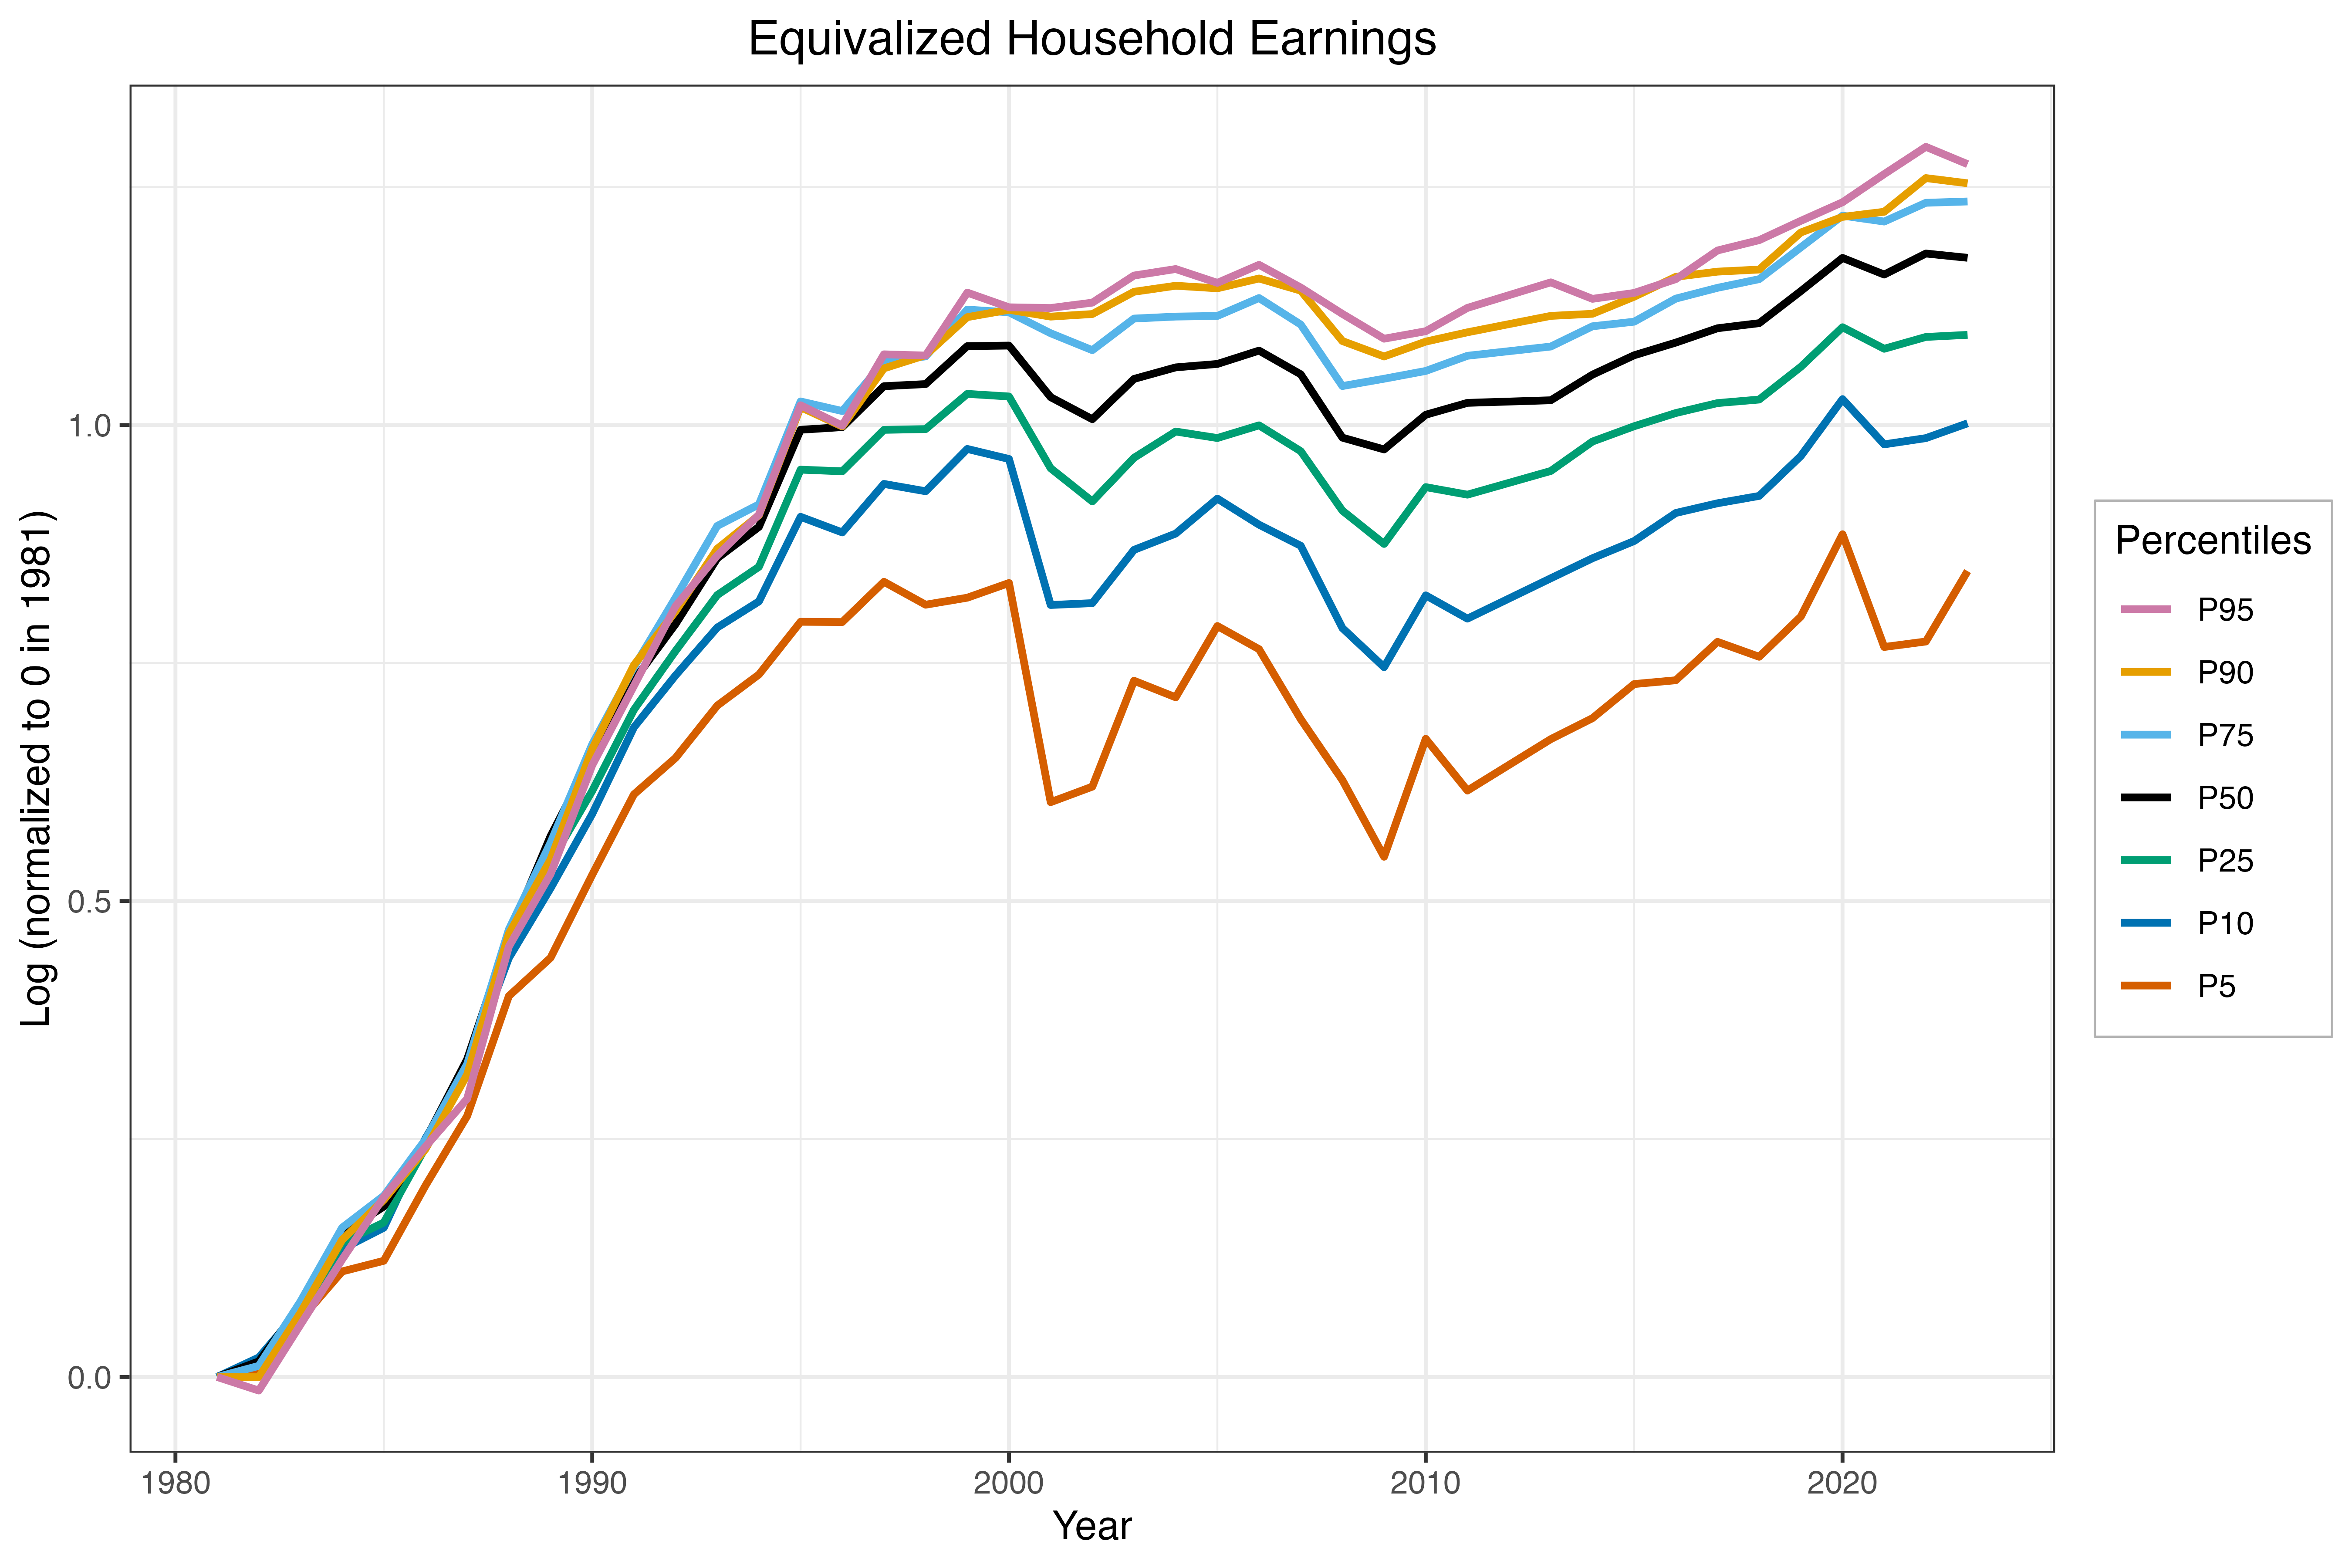
\includegraphics[width=0.88\textwidth]{figures/Fig_2/Fig_2_percentiles_1981.png}
    \caption{Percentiles of the Household Earnings Distribution, 1981 - 2023, Normalized to 1981}
    \label{fig:appendix_cyclic_earnings_1981}

    \vspace{2em} 

    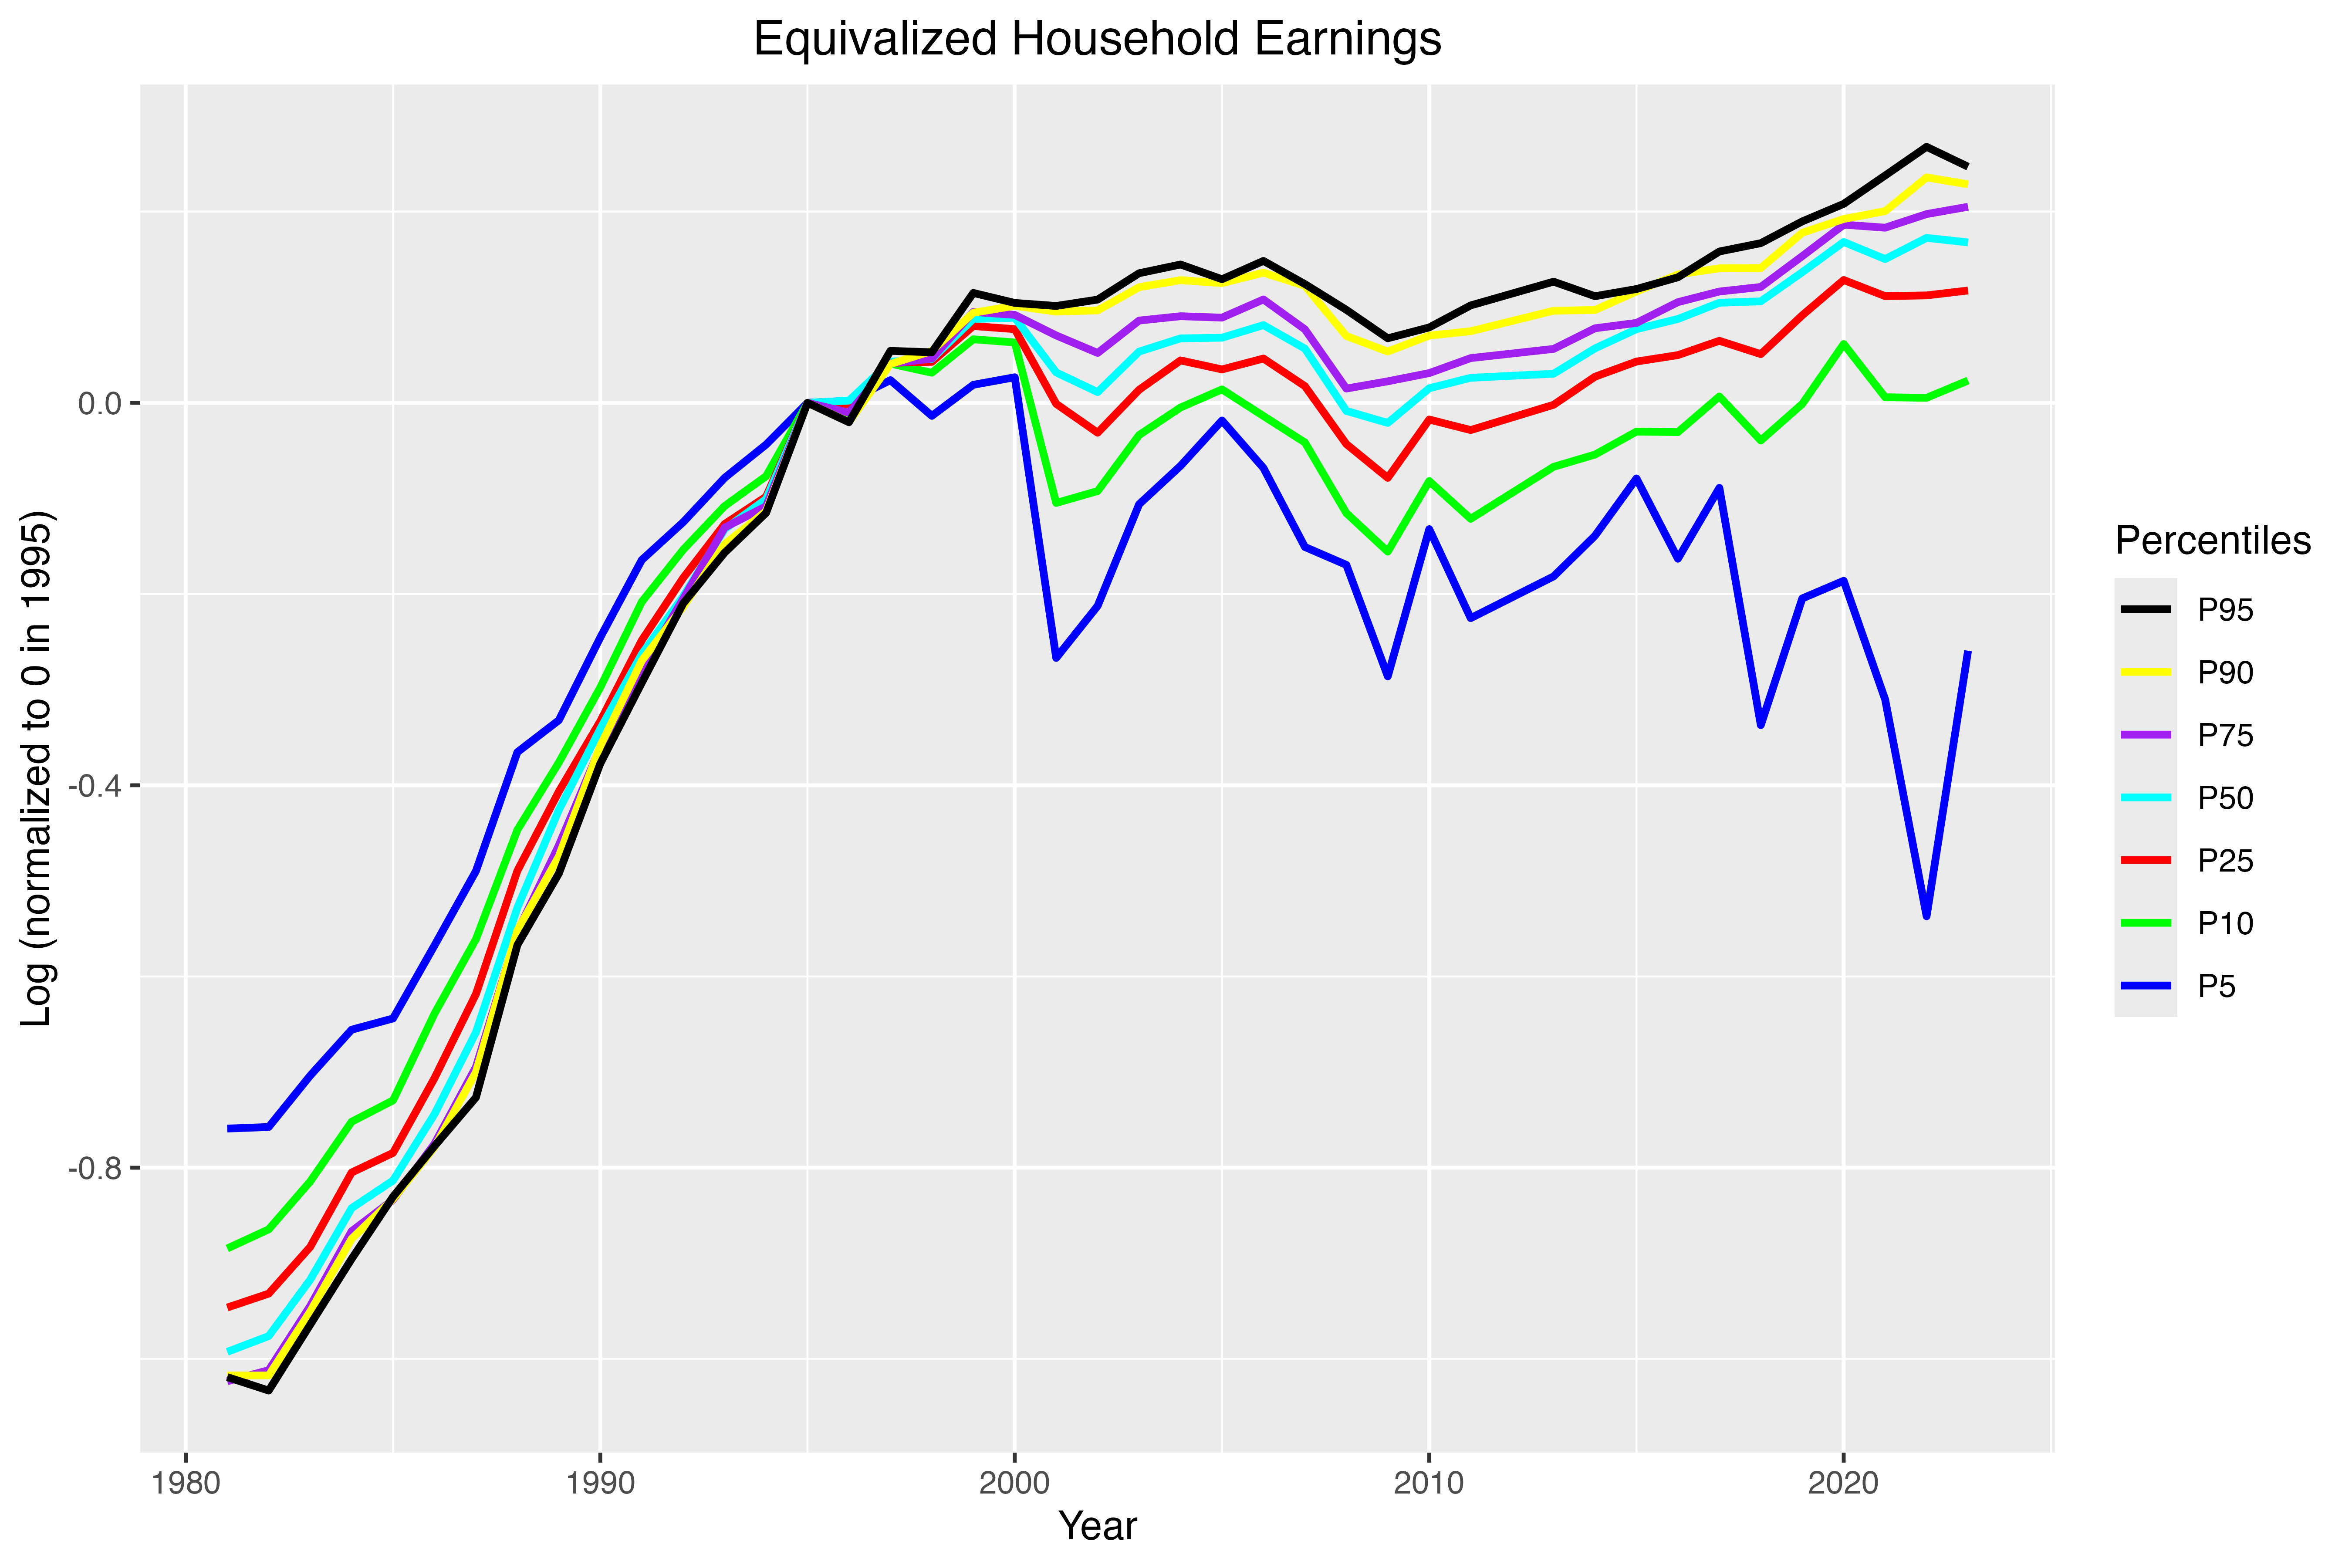
\includegraphics[width=0.88\textwidth]{figures/Fig_2/Fig_2_percentiles_1995.png}
    \caption{Percentiles of the Household Earnings Distribution, 1981 - 2023, Normalized to 1995}
    \label{fig:appendix_cyclic_earnings_1995}
\end{figure}

\begin{figure}[ht]
    \centering
    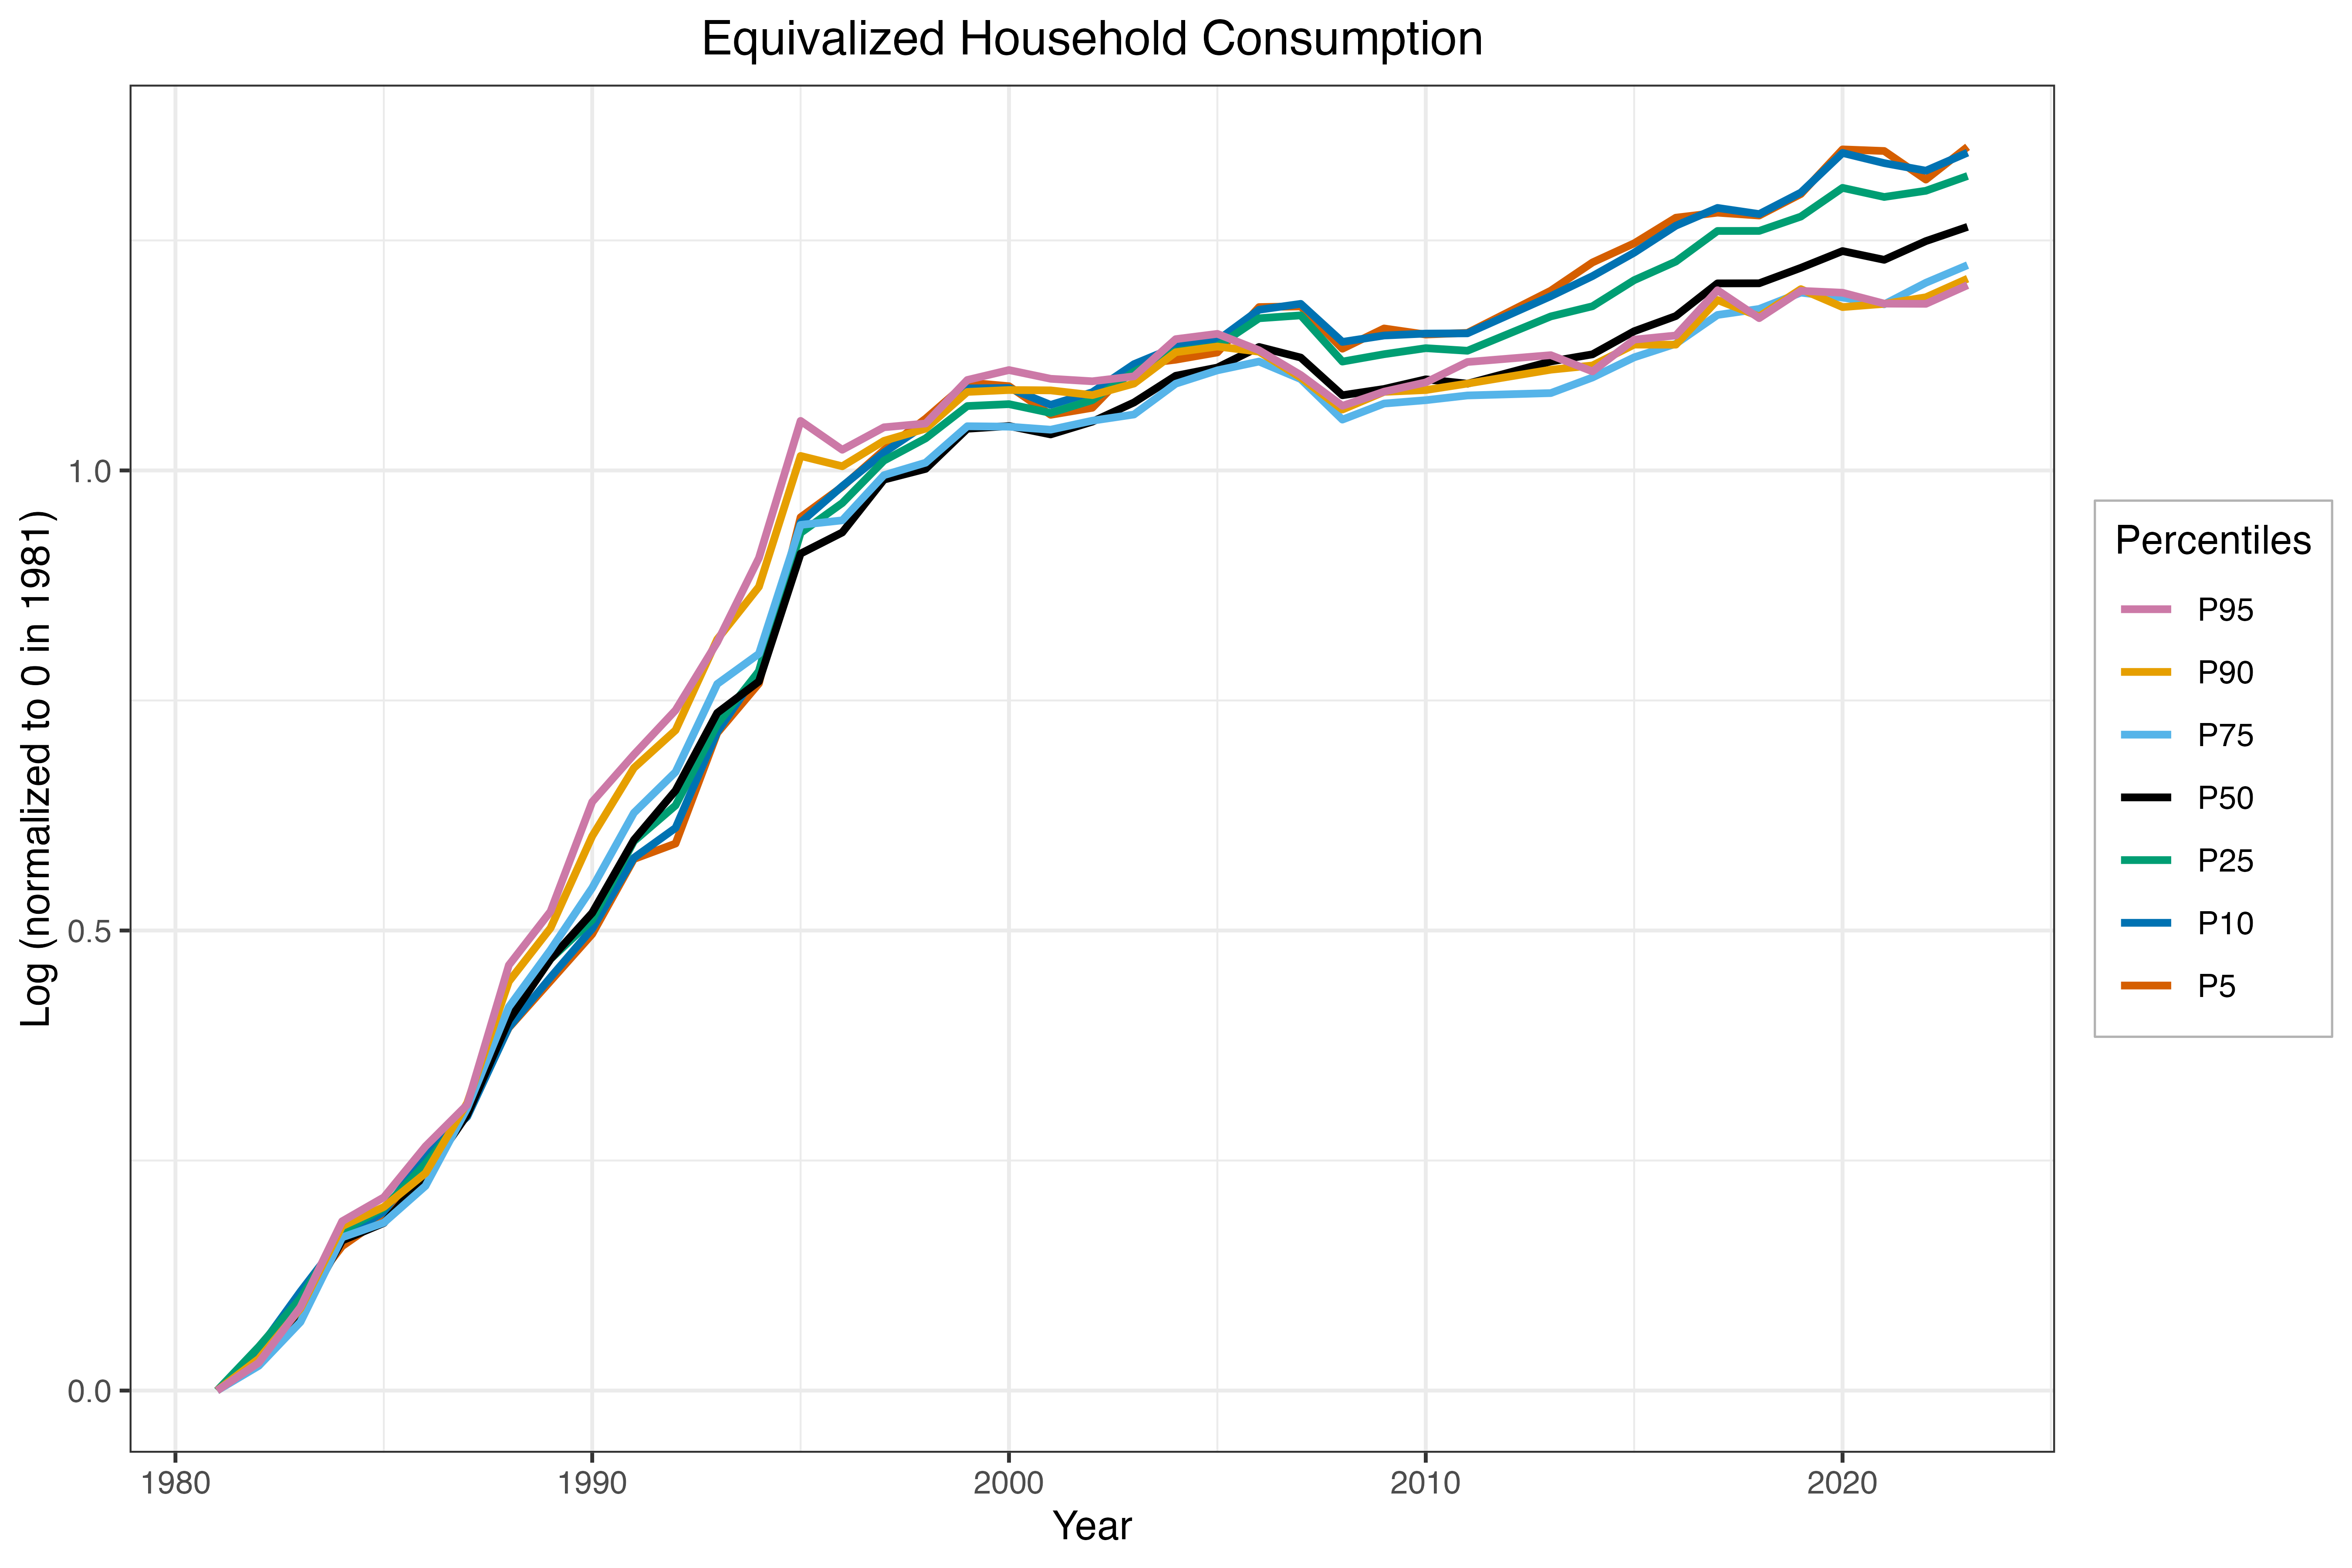
\includegraphics[width=0.88\textwidth]{figures/Fig_7/Fig_7_percentiles_1981.png}
    \caption{Percentiles of the Household Consumption Distribution, 1981 - 2023, Normalized to 1981}
    \label{fig:appendix_cyclic_consumption_1981}

    \vspace{2em} 

    \centering
    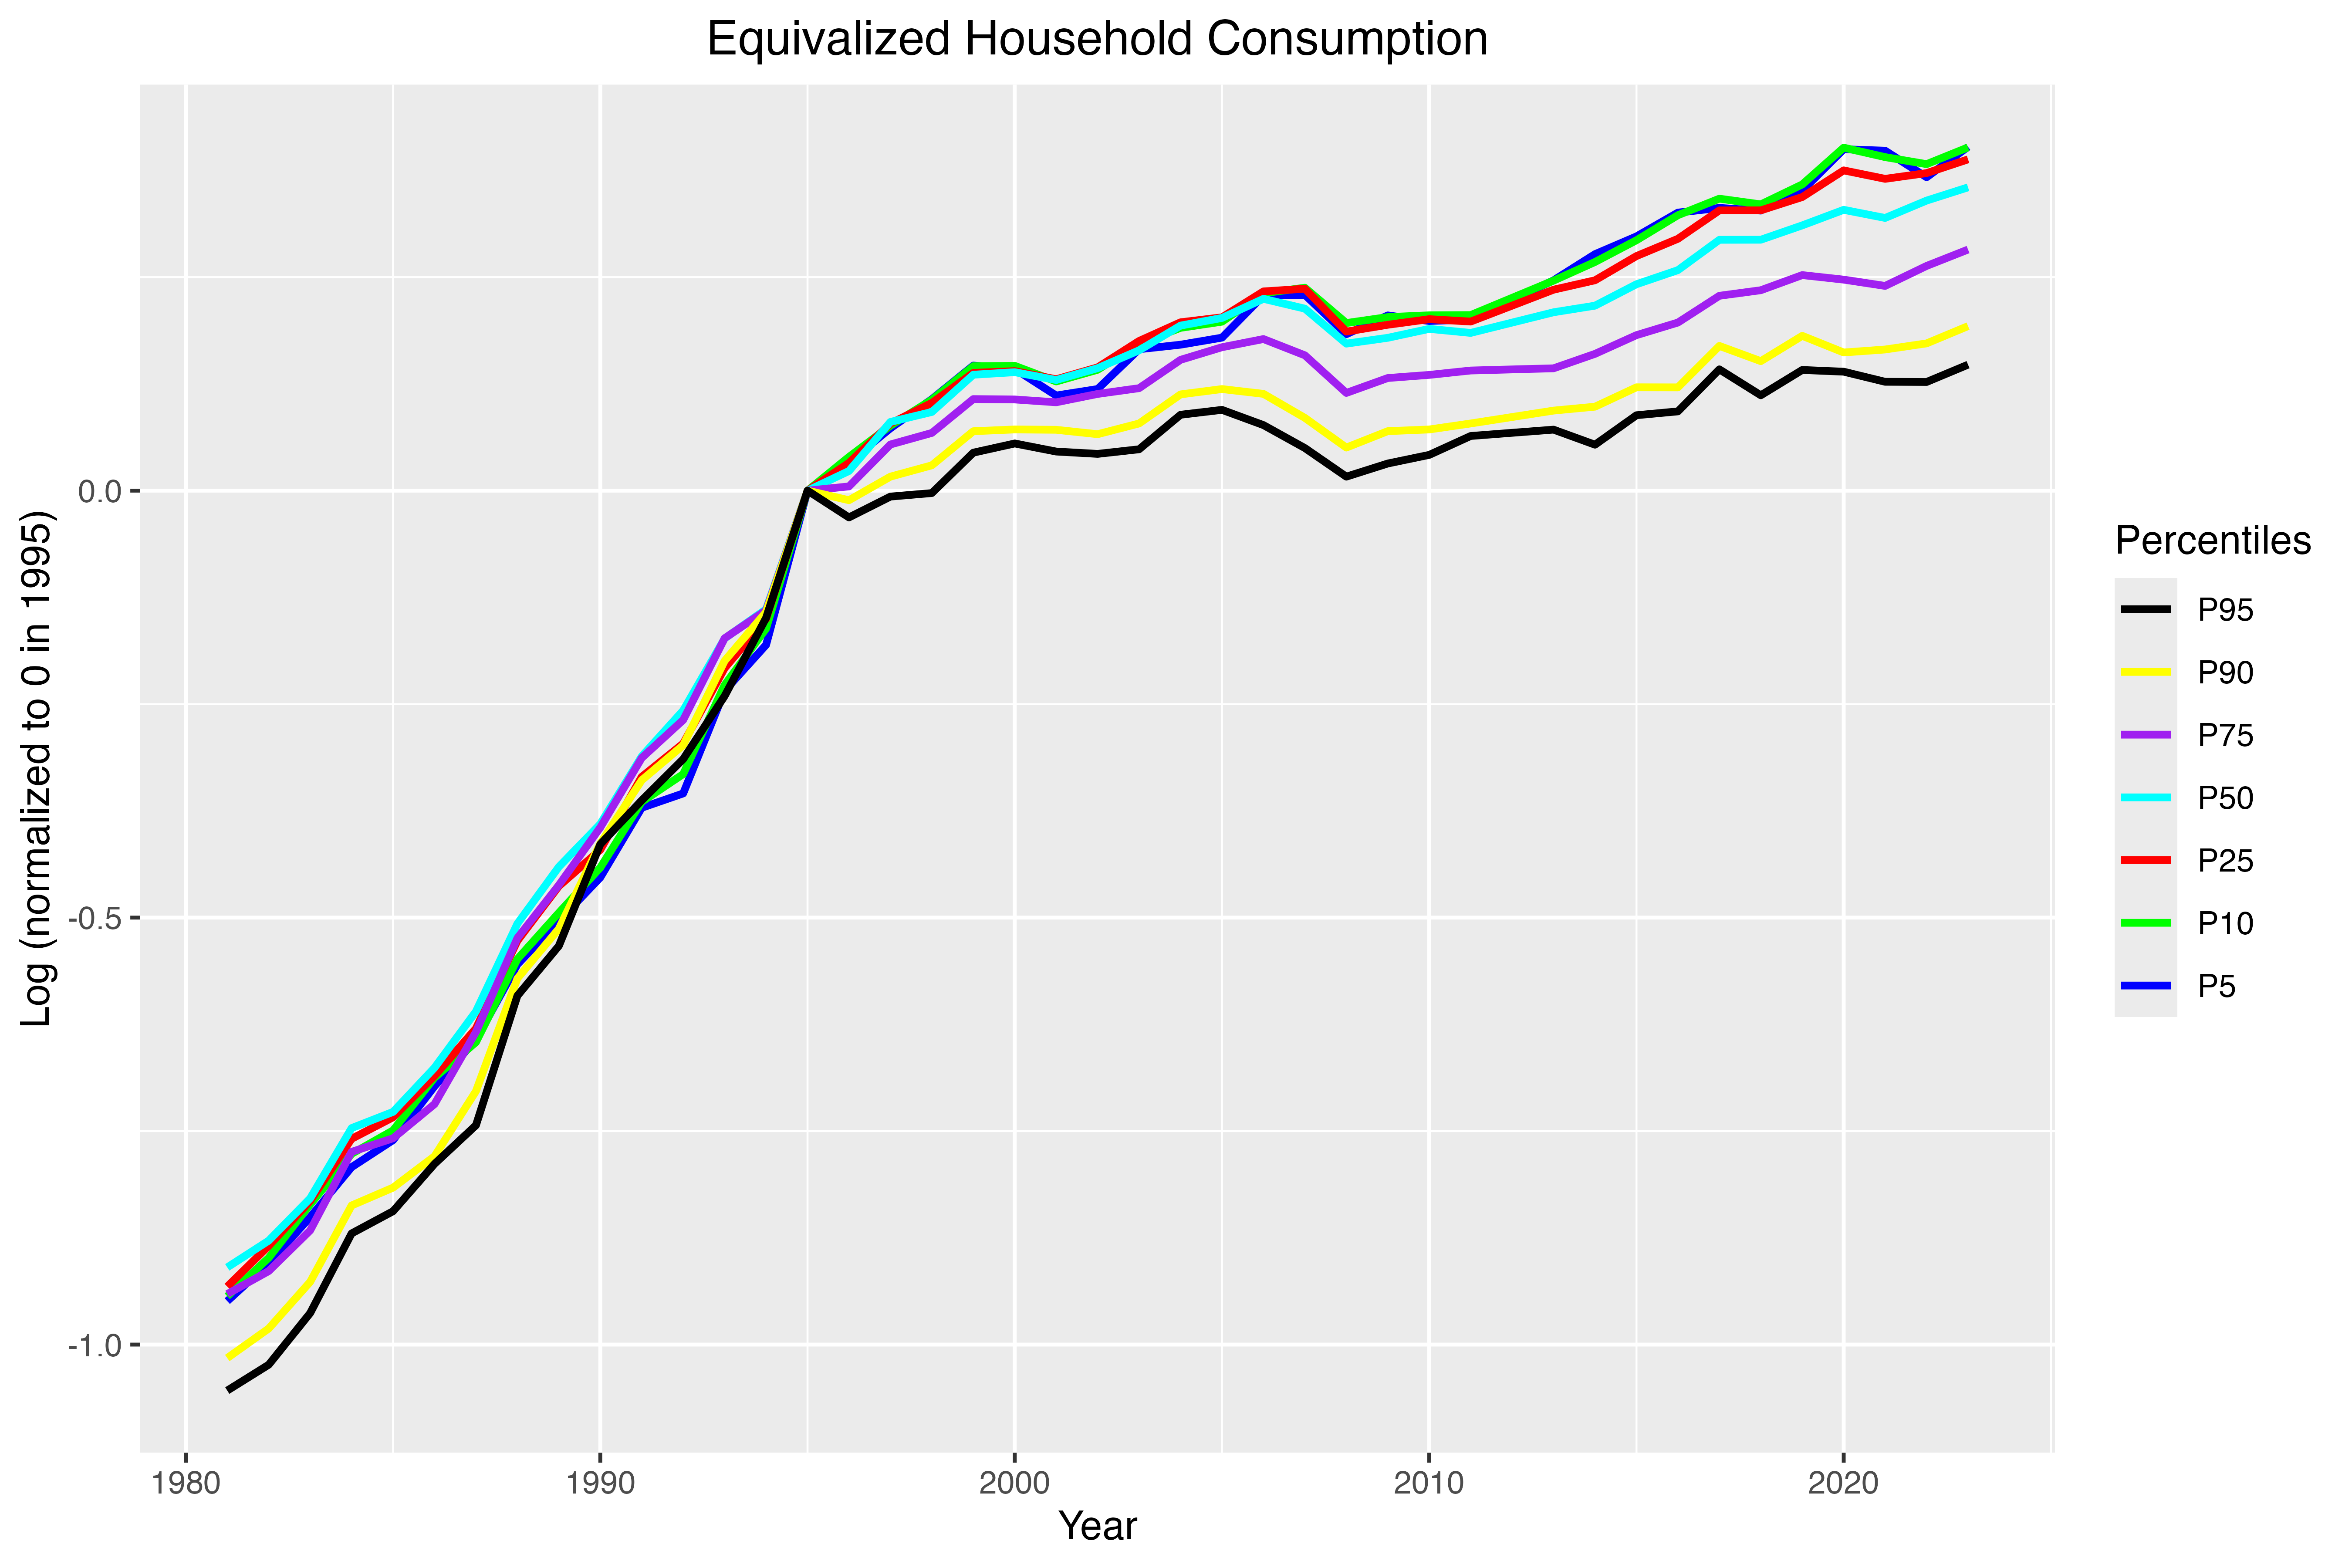
\includegraphics[width=0.88\textwidth]{figures/Fig_7/Fig_7_percentiles_1995.png}
    \caption{Percentiles of the Household Consumption Distribution, 1981 - 2023, Normalized to 1995}
    \label{fig:appendix_cyclic_consumption_1995}
\end{figure}

\clearpage

\begin{figure}[t]
    \centering
    \begin{subfigure}[t]{0.495\textwidth}
        \centering
        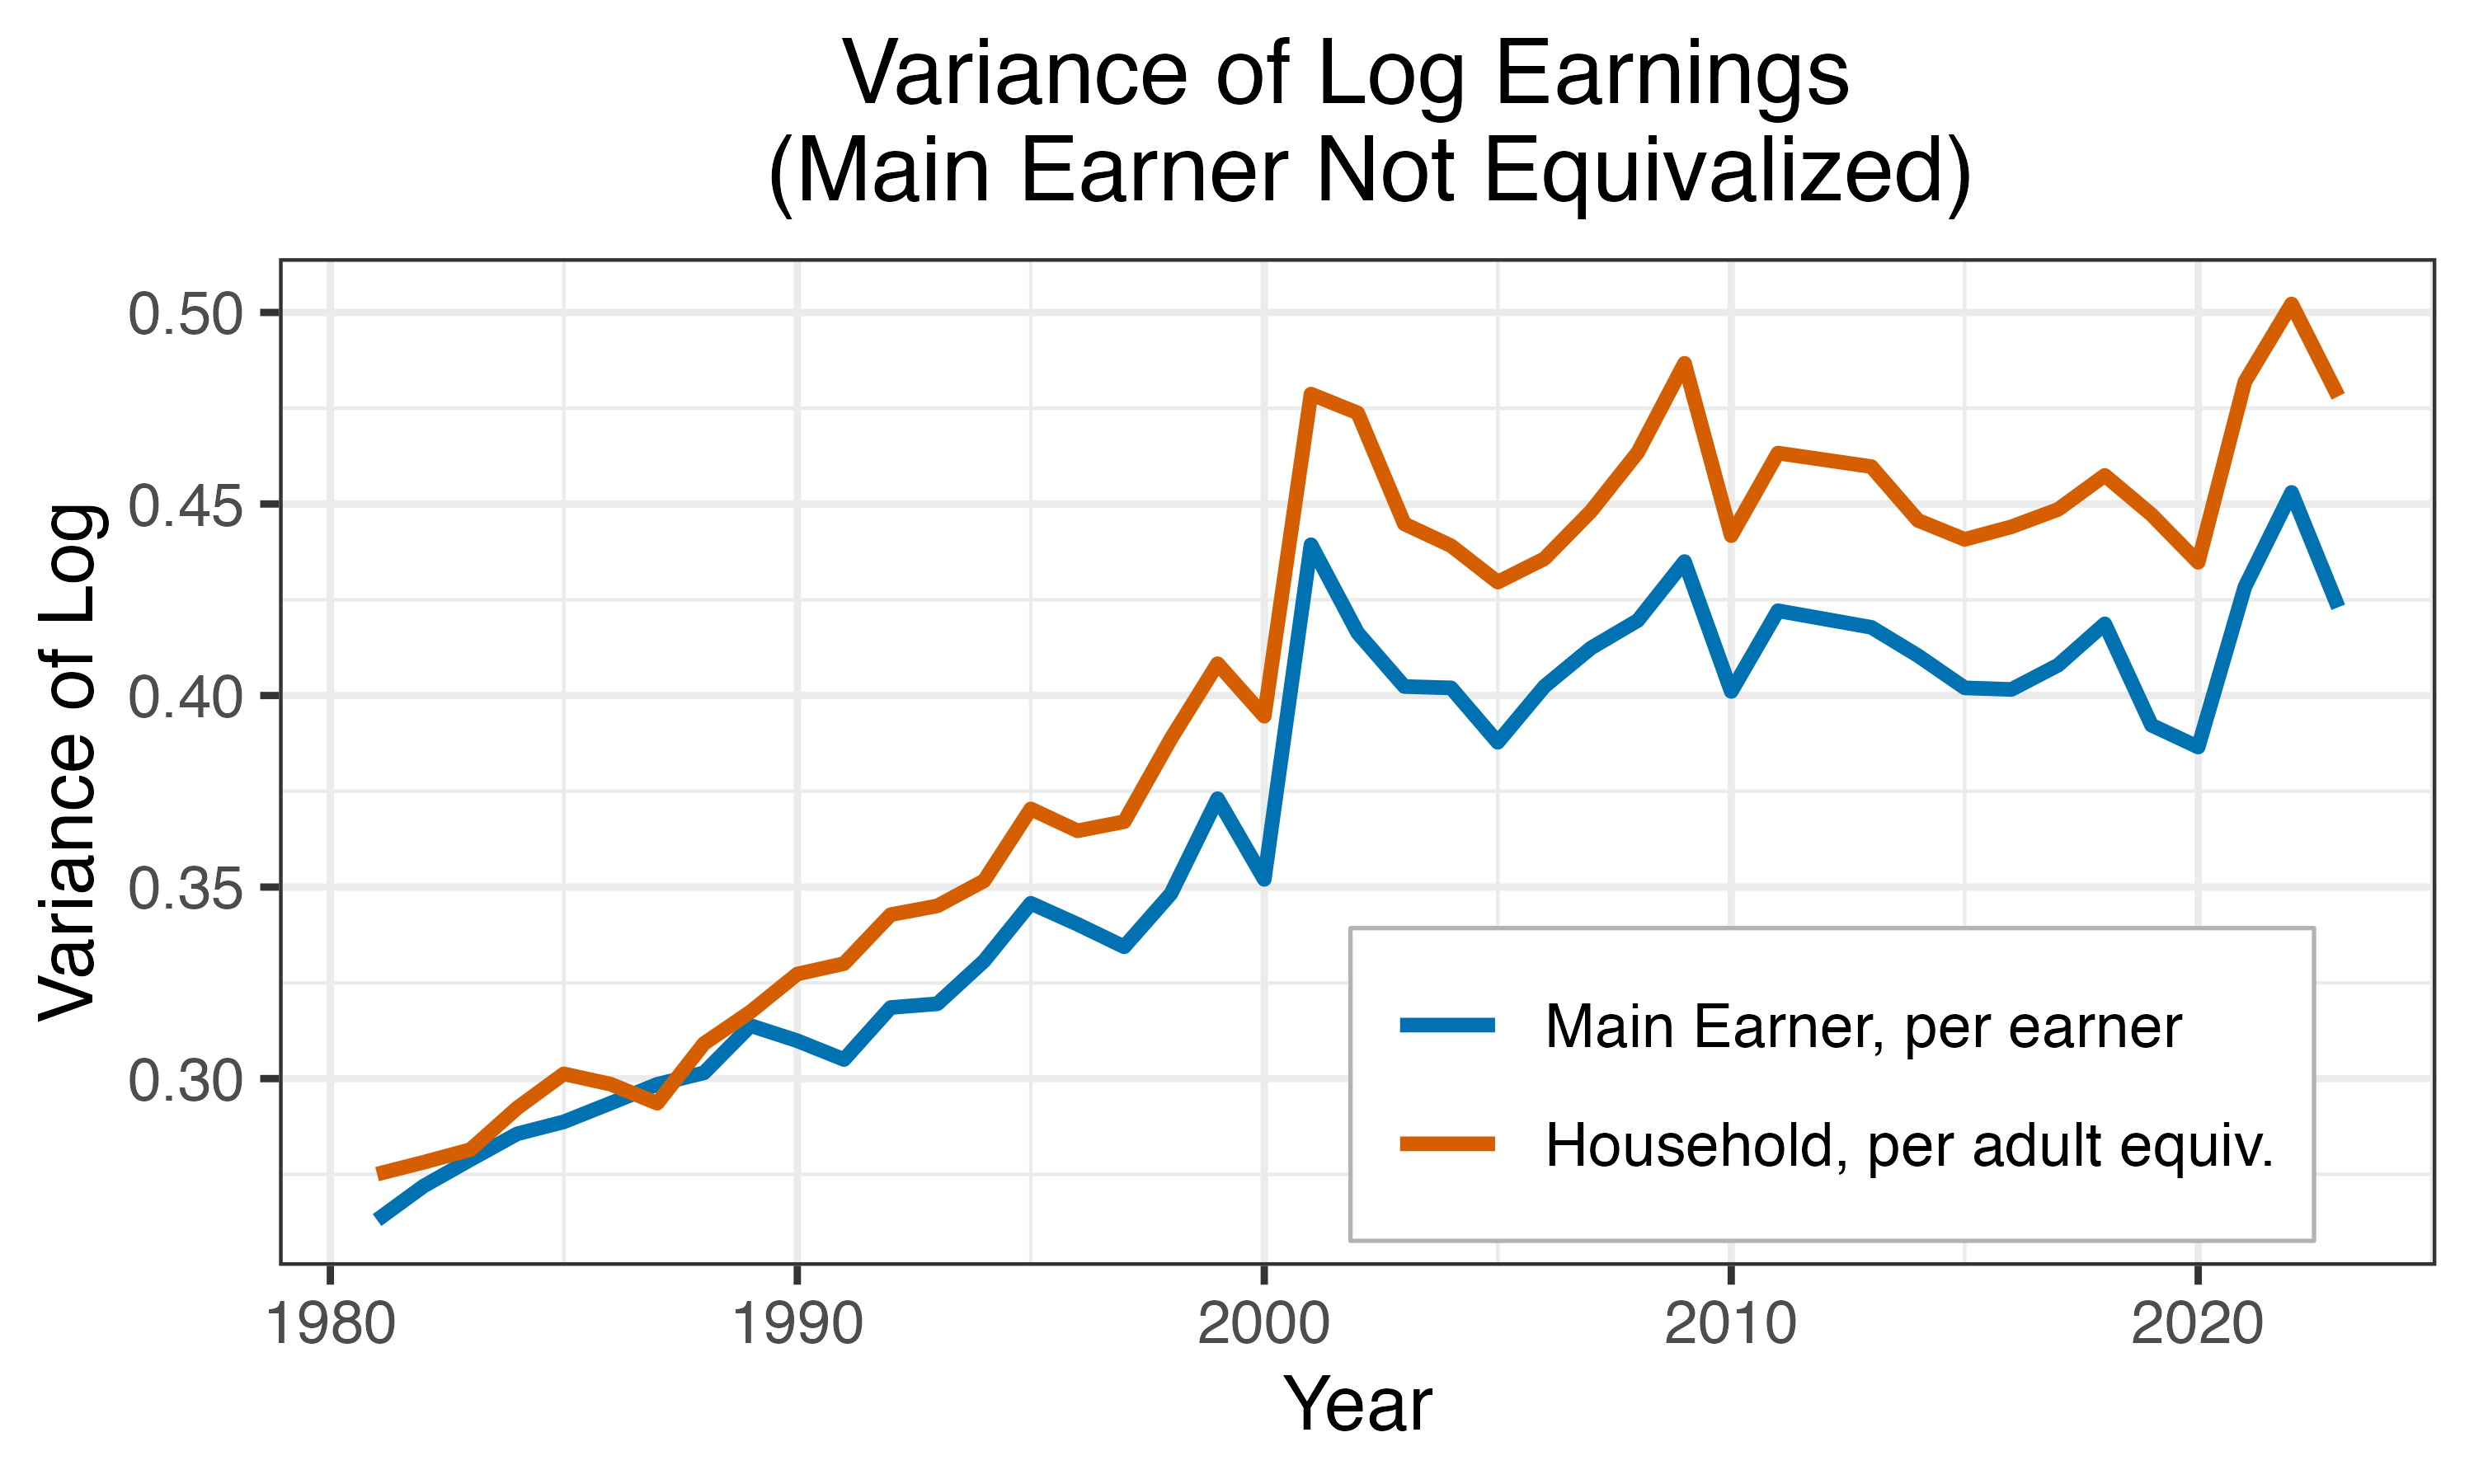
\includegraphics[width=\textwidth]{figures/Fig_3/Fig_3g_Var_indHH_raw.png}
    \end{subfigure}
    \begin{subfigure}[t]{0.495\textwidth}
        \centering
        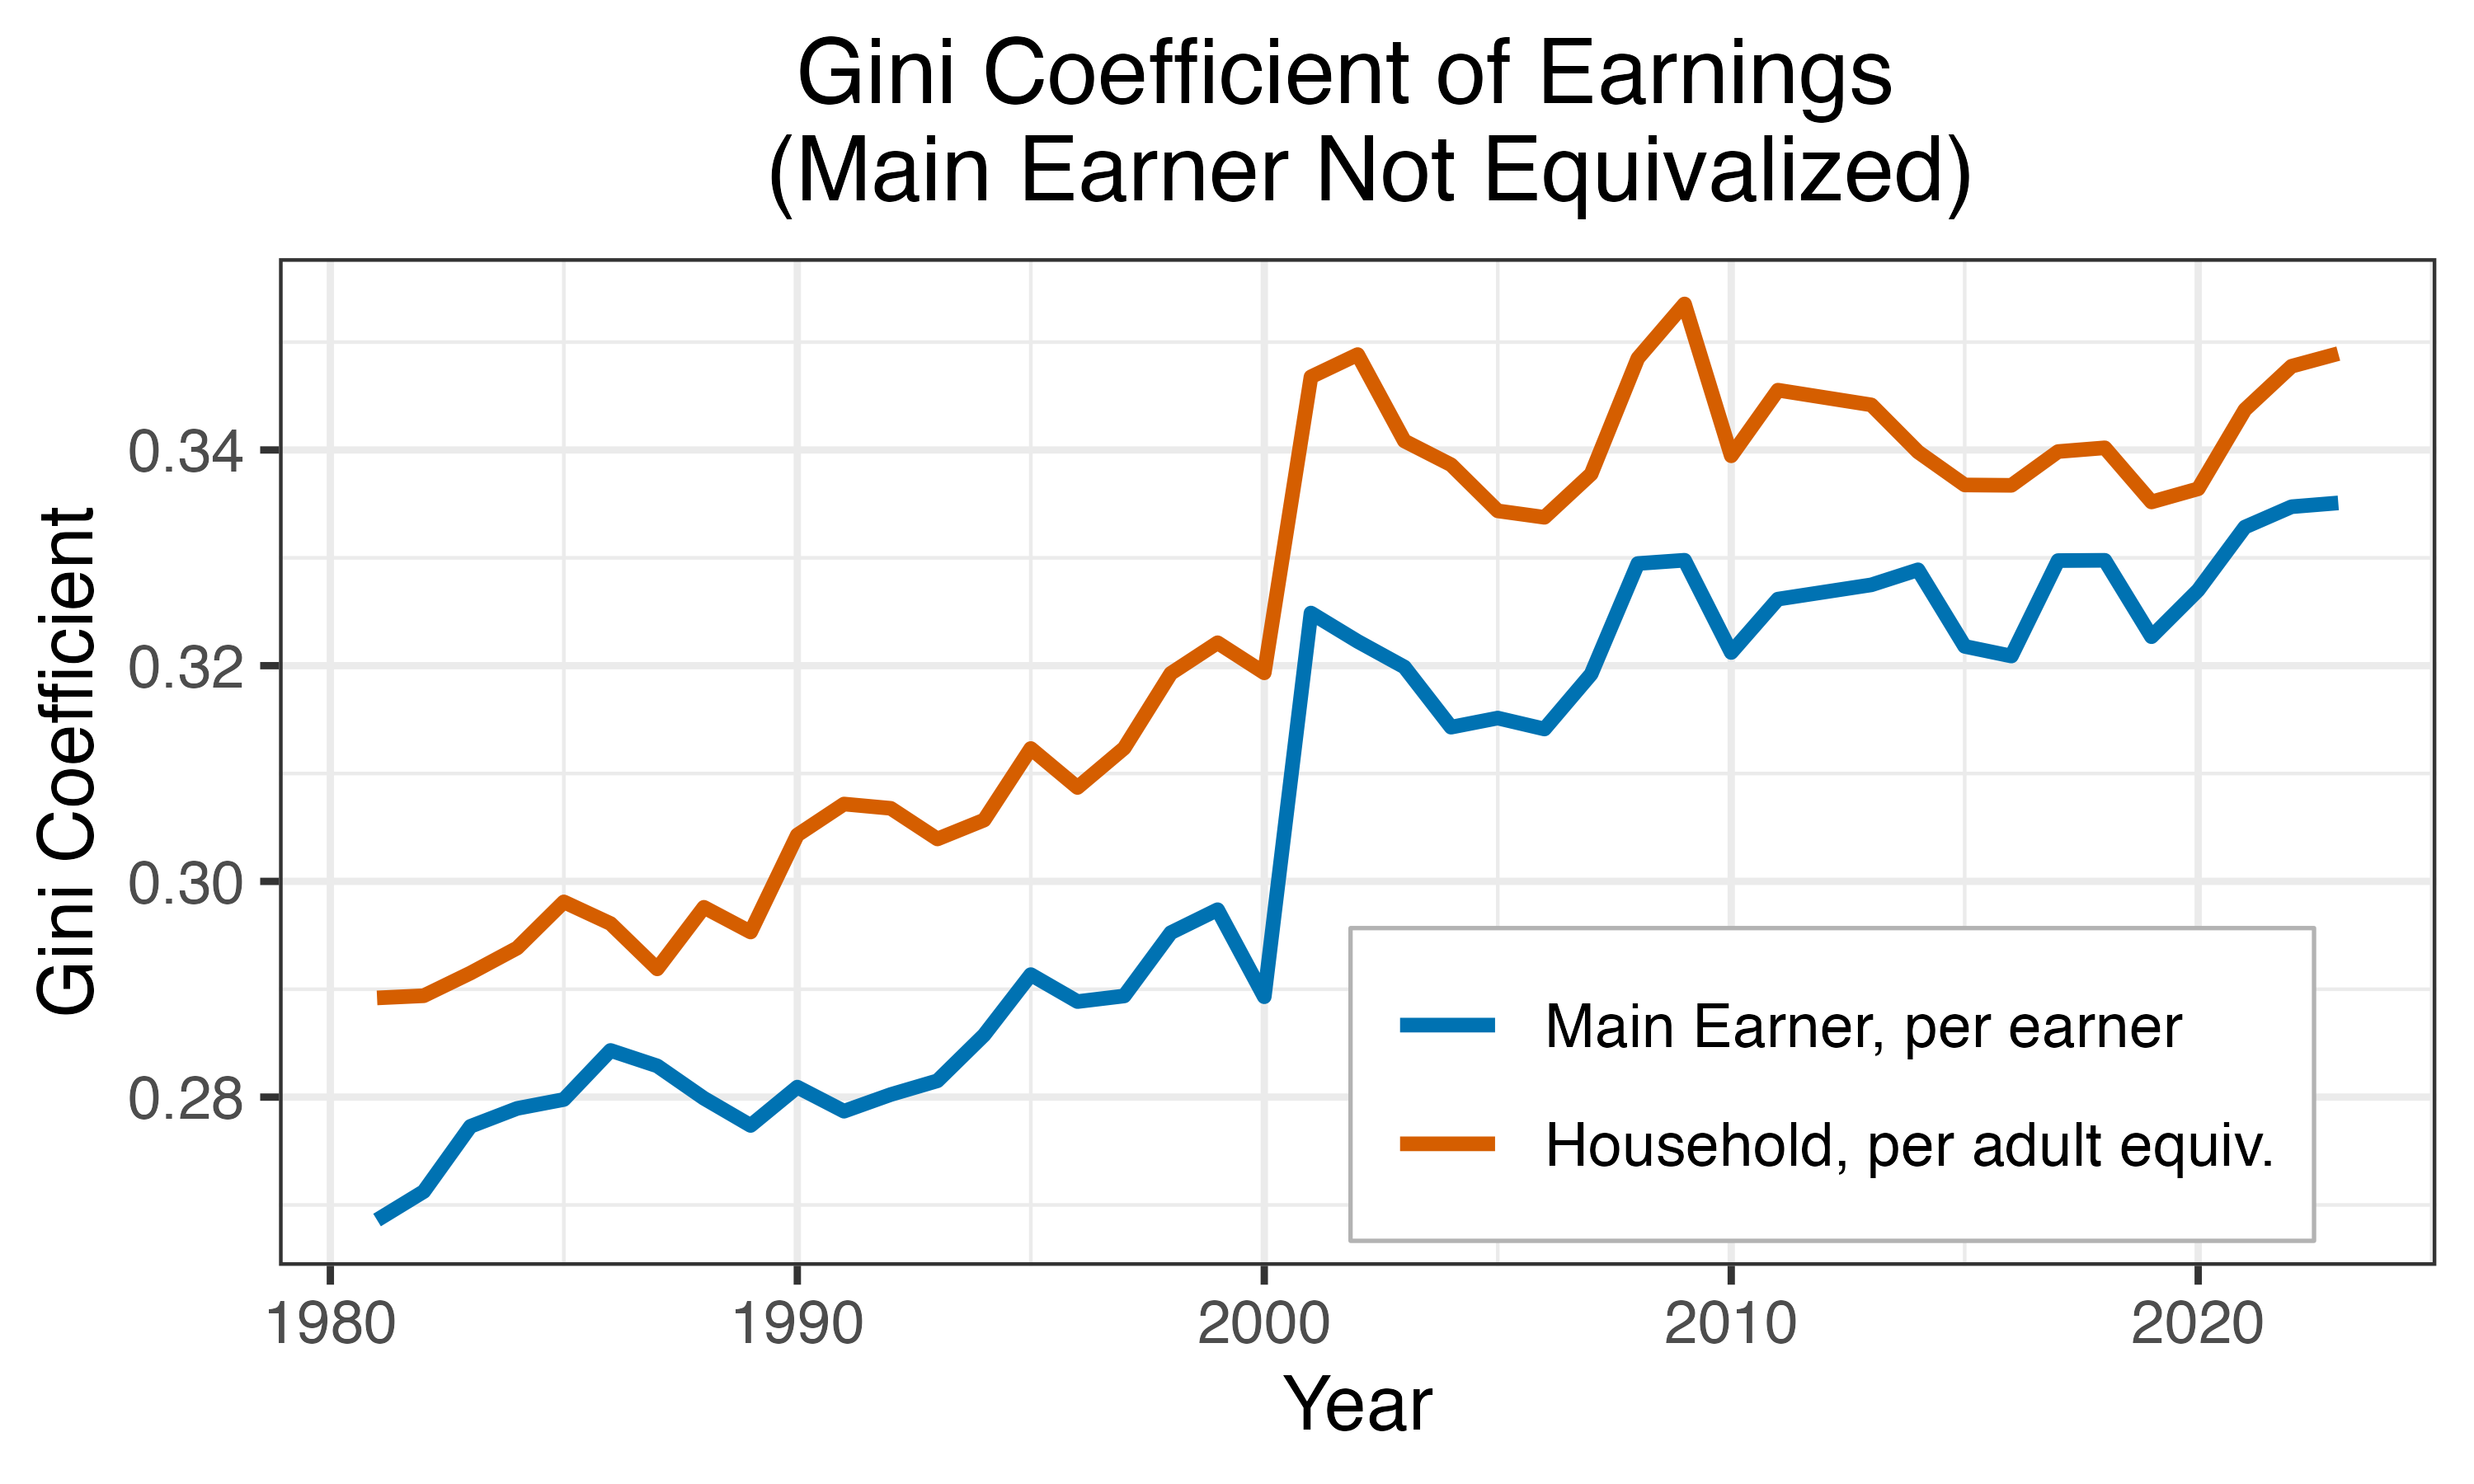
\includegraphics[width=\textwidth]{figures/Fig_3/Fig_3h_Gini_indHH_raw.png}
    \end{subfigure}
    \caption{Main Earner and Household Earnings Inequality, Main Earner Not Equivalized}
    \label{fig:appendix_indHH_raw}
\end{figure}

\section{The Floor at 5\% of the Median}
\label{sec:appendix_sample}

Figure \ref{fig:appendix_sample} compares household earnings inequality on all households with positive earnings and on the earnings sample of Section \ref{sec:sample}. The two variance series stay within 0.1 of each other until 2015 and then separate. On all positive earners, the variance jumps to 0.96 in 2018 and 1.12 in 2022, while on the earnings sample it stays between 0.43 and 0.50. The two Gini series differ by at most 0.004 before 2016 and at most 0.014 after, which is small compared with the difference in the variance.

% The lognormal distribution gives a way to check which pair of numbers is consistent. Under lognormality a Gini coefficient of $G$ implies a variance of logs of $2\left[\Phi^{-1}\left((1+G)/2\right)\right]^2$, where $\Phi$ is the standard normal distribution function. In 2023 the Gini of 0.362 on all positive earners implies a variance of 0.44, against a measured 0.97. On the earnings sample the Gini of 0.349 implies 0.41, against a measured 0.48.

\begin{figure}[!h]
    \centering
    \begin{subfigure}[t]{0.495\textwidth}
        \centering
        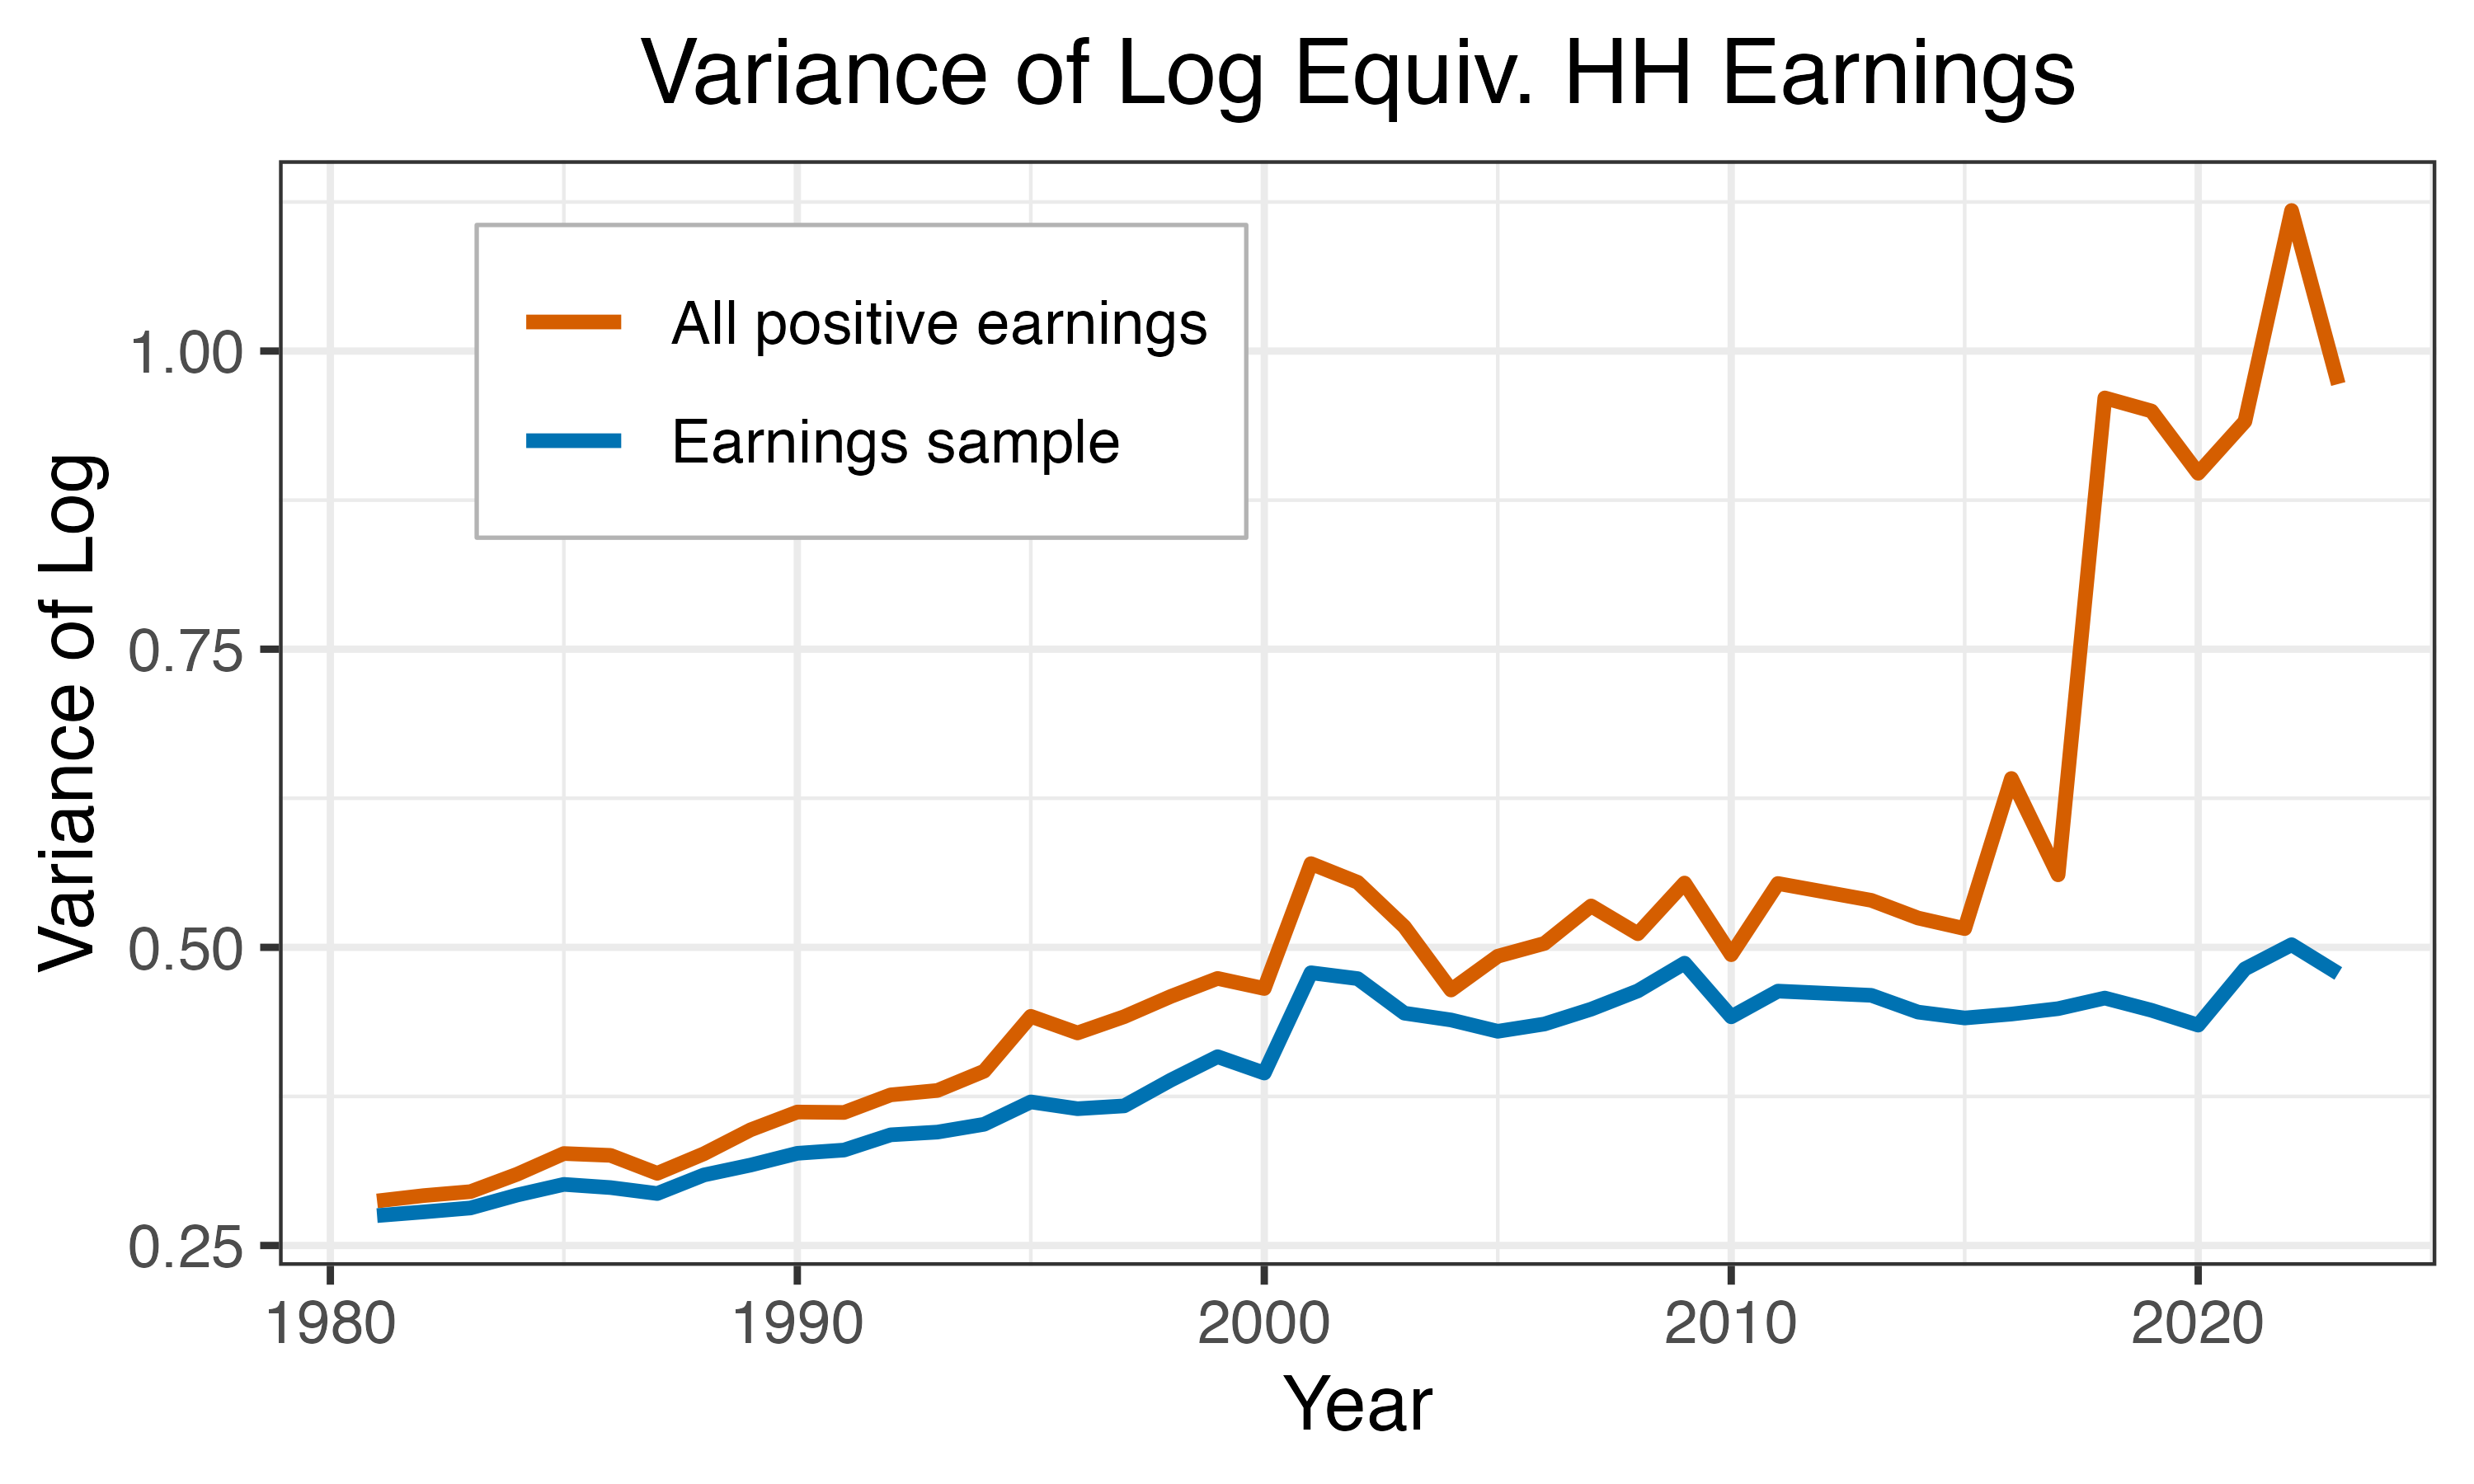
\includegraphics[width=\textwidth]{figures/Fig_1/Fig_1e_Var_trim.png}
    \end{subfigure}
    \begin{subfigure}[t]{0.495\textwidth}
        \centering
        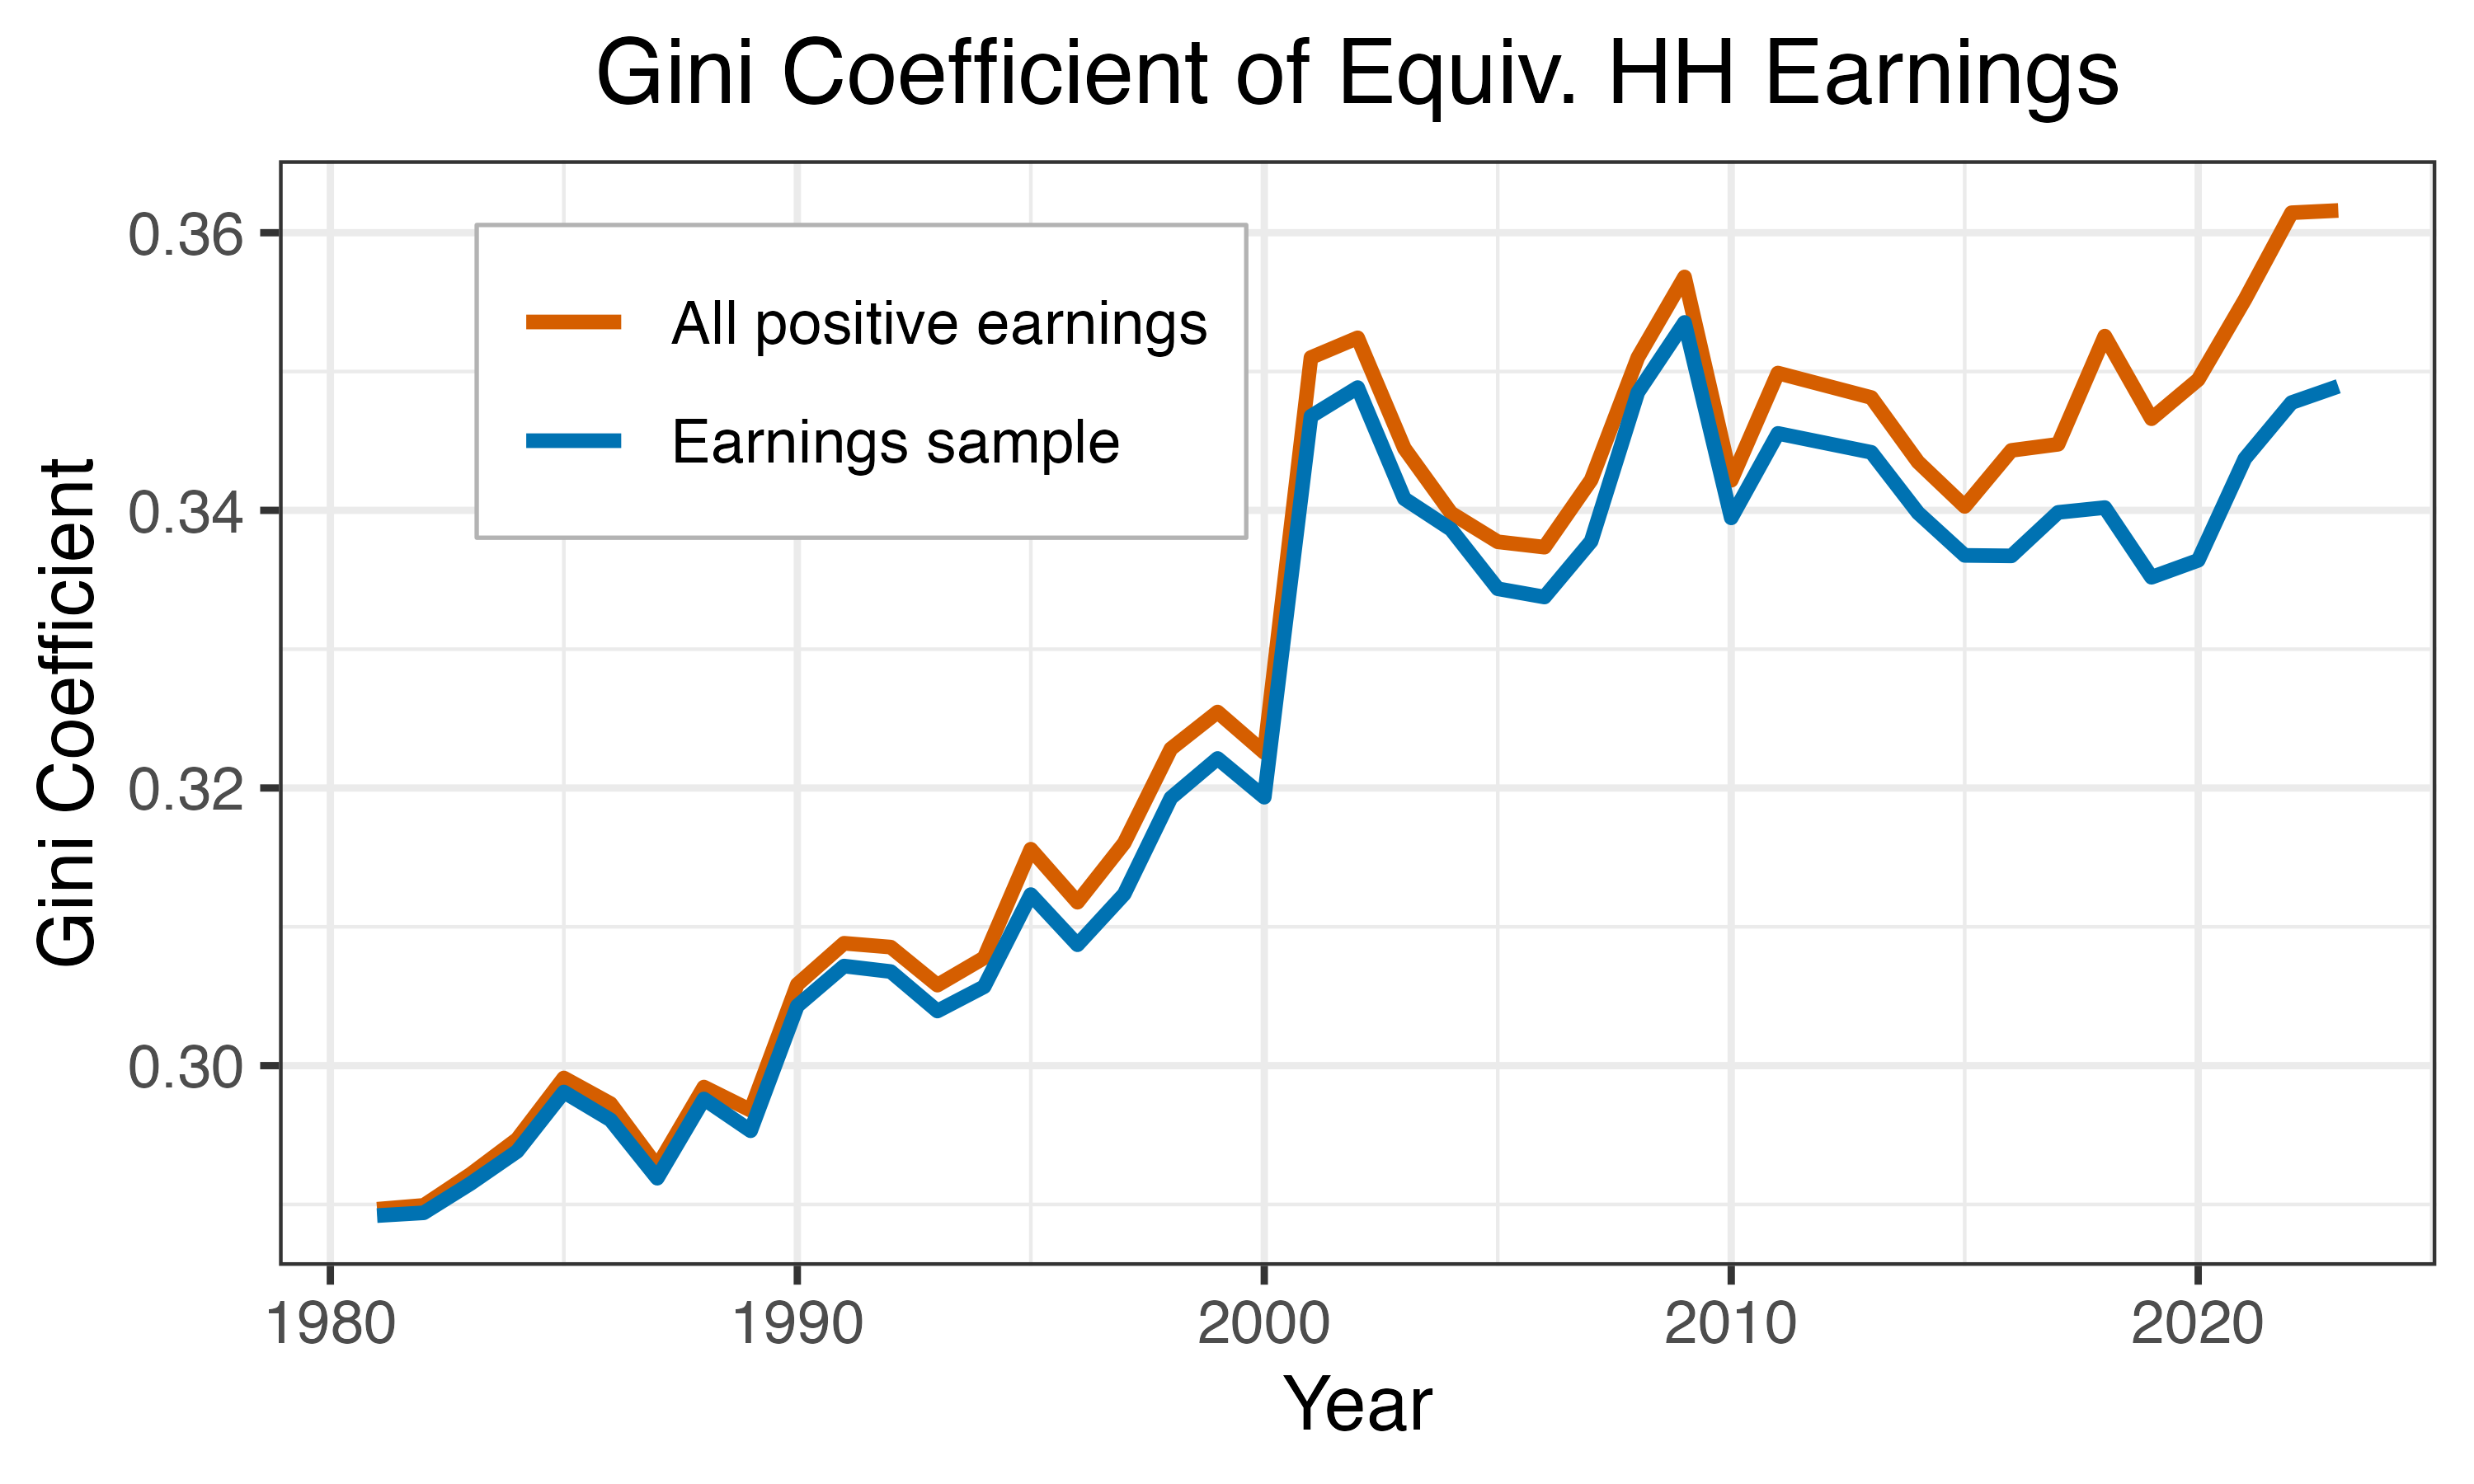
\includegraphics[width=\textwidth]{figures/Fig_1/Fig_1f_Gini_trim.png}
    \end{subfigure}
    \caption{Household Earnings Inequality With and Without the Earnings Sample Restriction}
    \label{fig:appendix_sample}
\end{figure}

Table \ref{tab:appendix_floor} repeats the comparison for every series. The floor matters most where many values sit close to zero. For the individual earnings series it lowers the 2023 variance of logs from between 0.80 and 1.22 to between 0.42 and 0.47. For earnings plus asset income, households without earnings and with little asset income push the 2023 variance to 3.61 without the threshold, against 0.72 with it. For pre-tax and disposable income, consumption, food and housing, the floor removes at most 0.08\% of households in any year and changes the variance of logs by less than 0.01 and the Gini by less than 0.001.

\begin{table}[ht]
    \centering
    \small
    \caption{The Floor at 5\% of the Median, Series by Series}
    \label{tab:appendix_floor}
    \begin{tabular}{lcccccc}
        \toprule
         & \multicolumn{2}{c}{Share removed (\%)} & \multicolumn{2}{c}{Var.\ of logs, 2023} & \multicolumn{2}{c}{Largest reduction} \\
        \cmidrule(lr){2-3} \cmidrule(lr){4-5} \cmidrule(lr){6-7}
        Series & All years & Peak year & No floor & Floor & Var. & Gini \\
        \midrule
        Household earnings & 0.64 & 2.24 & 0.97 & 0.48 & 0.616 & 0.014 \\
        Main earner, per adult equiv. & 0.38 & 1.37 & 0.80 & 0.47 & 0.390 & 0.008 \\
        Main earner, per earner & 0.63 & 1.80 & 0.83 & 0.42 & 0.479 & 0.011 \\
        Household head, per earner & 0.65 & 1.66 & 0.81 & 0.43 & 0.409 & 0.010 \\
        Spouse, per earner & 0.86 & 3.45 & 1.22 & 0.43 & 1.051 & 0.023 \\
        Earnings + private transfers & 0.32 & 0.55 & 0.44 & 0.41 & 0.090 & 0.004 \\
        Earnings + asset income & 6.02 & 14.19 & 3.61 & 0.72 & 3.502 & 0.084 \\
        Earnings + transfers + asset income & 0.13 & 0.26 & 0.39 & 0.38 & 0.050 & 0.002 \\
        Pre-government income & 0.08 & 0.21 & 0.34 & 0.34 & 0.037 & 0.001 \\
        Pre-tax income & $<$0.01 & 0.01 & 0.26 & 0.26 & 0.002 & $<$0.001 \\
        Disposable income & $<$0.01 & 0.02 & 0.25 & 0.25 & 0.004 & $<$0.001 \\
        Consumption & $<$0.01 & 0.01 & 0.15 & 0.15 & 0.001 & $<$0.001 \\
        Food & $<$0.01 & 0.02 & 0.09 & 0.09 & 0.003 & $<$0.001 \\
        Housing services & 0.01 & 0.08 & 0.34 & 0.34 & 0.008 & $<$0.001 \\
        \bottomrule
    \end{tabular}

    % \medskip
    % \begin{minipage}{0.95\textwidth}
    %     \footnotesize
    %     \textit{Notes:} Share removed is the share of households with a positive value of the series that fall below 5\% of that year's weighted median of the same series, over all years and in the year where it is largest. Largest reduction is the largest fall in the variance of logs or the Gini coefficient in any single year when the floor is applied. The main earner is the household member with the highest earnings. The household head and spouse series are those used for the two-earner share and the between-spouse correlation; the spouse series starts in 1988.
    % \end{minipage}
\end{table}

\section{Private Transfers and Asset Income}
\label{sec:appendix_corr}

Figure \ref{fig:appendix_corr} plots the correlation between equivalized private transfers and equivalized asset income among households that receive either. It is computed from levels, without the floor, and covers every household that receives either. The correlation lies between $0.00$ and $0.08$, so the size of a household's private transfers is almost unrelated to the size of its asset income.

\begin{figure}[ht]
    \centering
    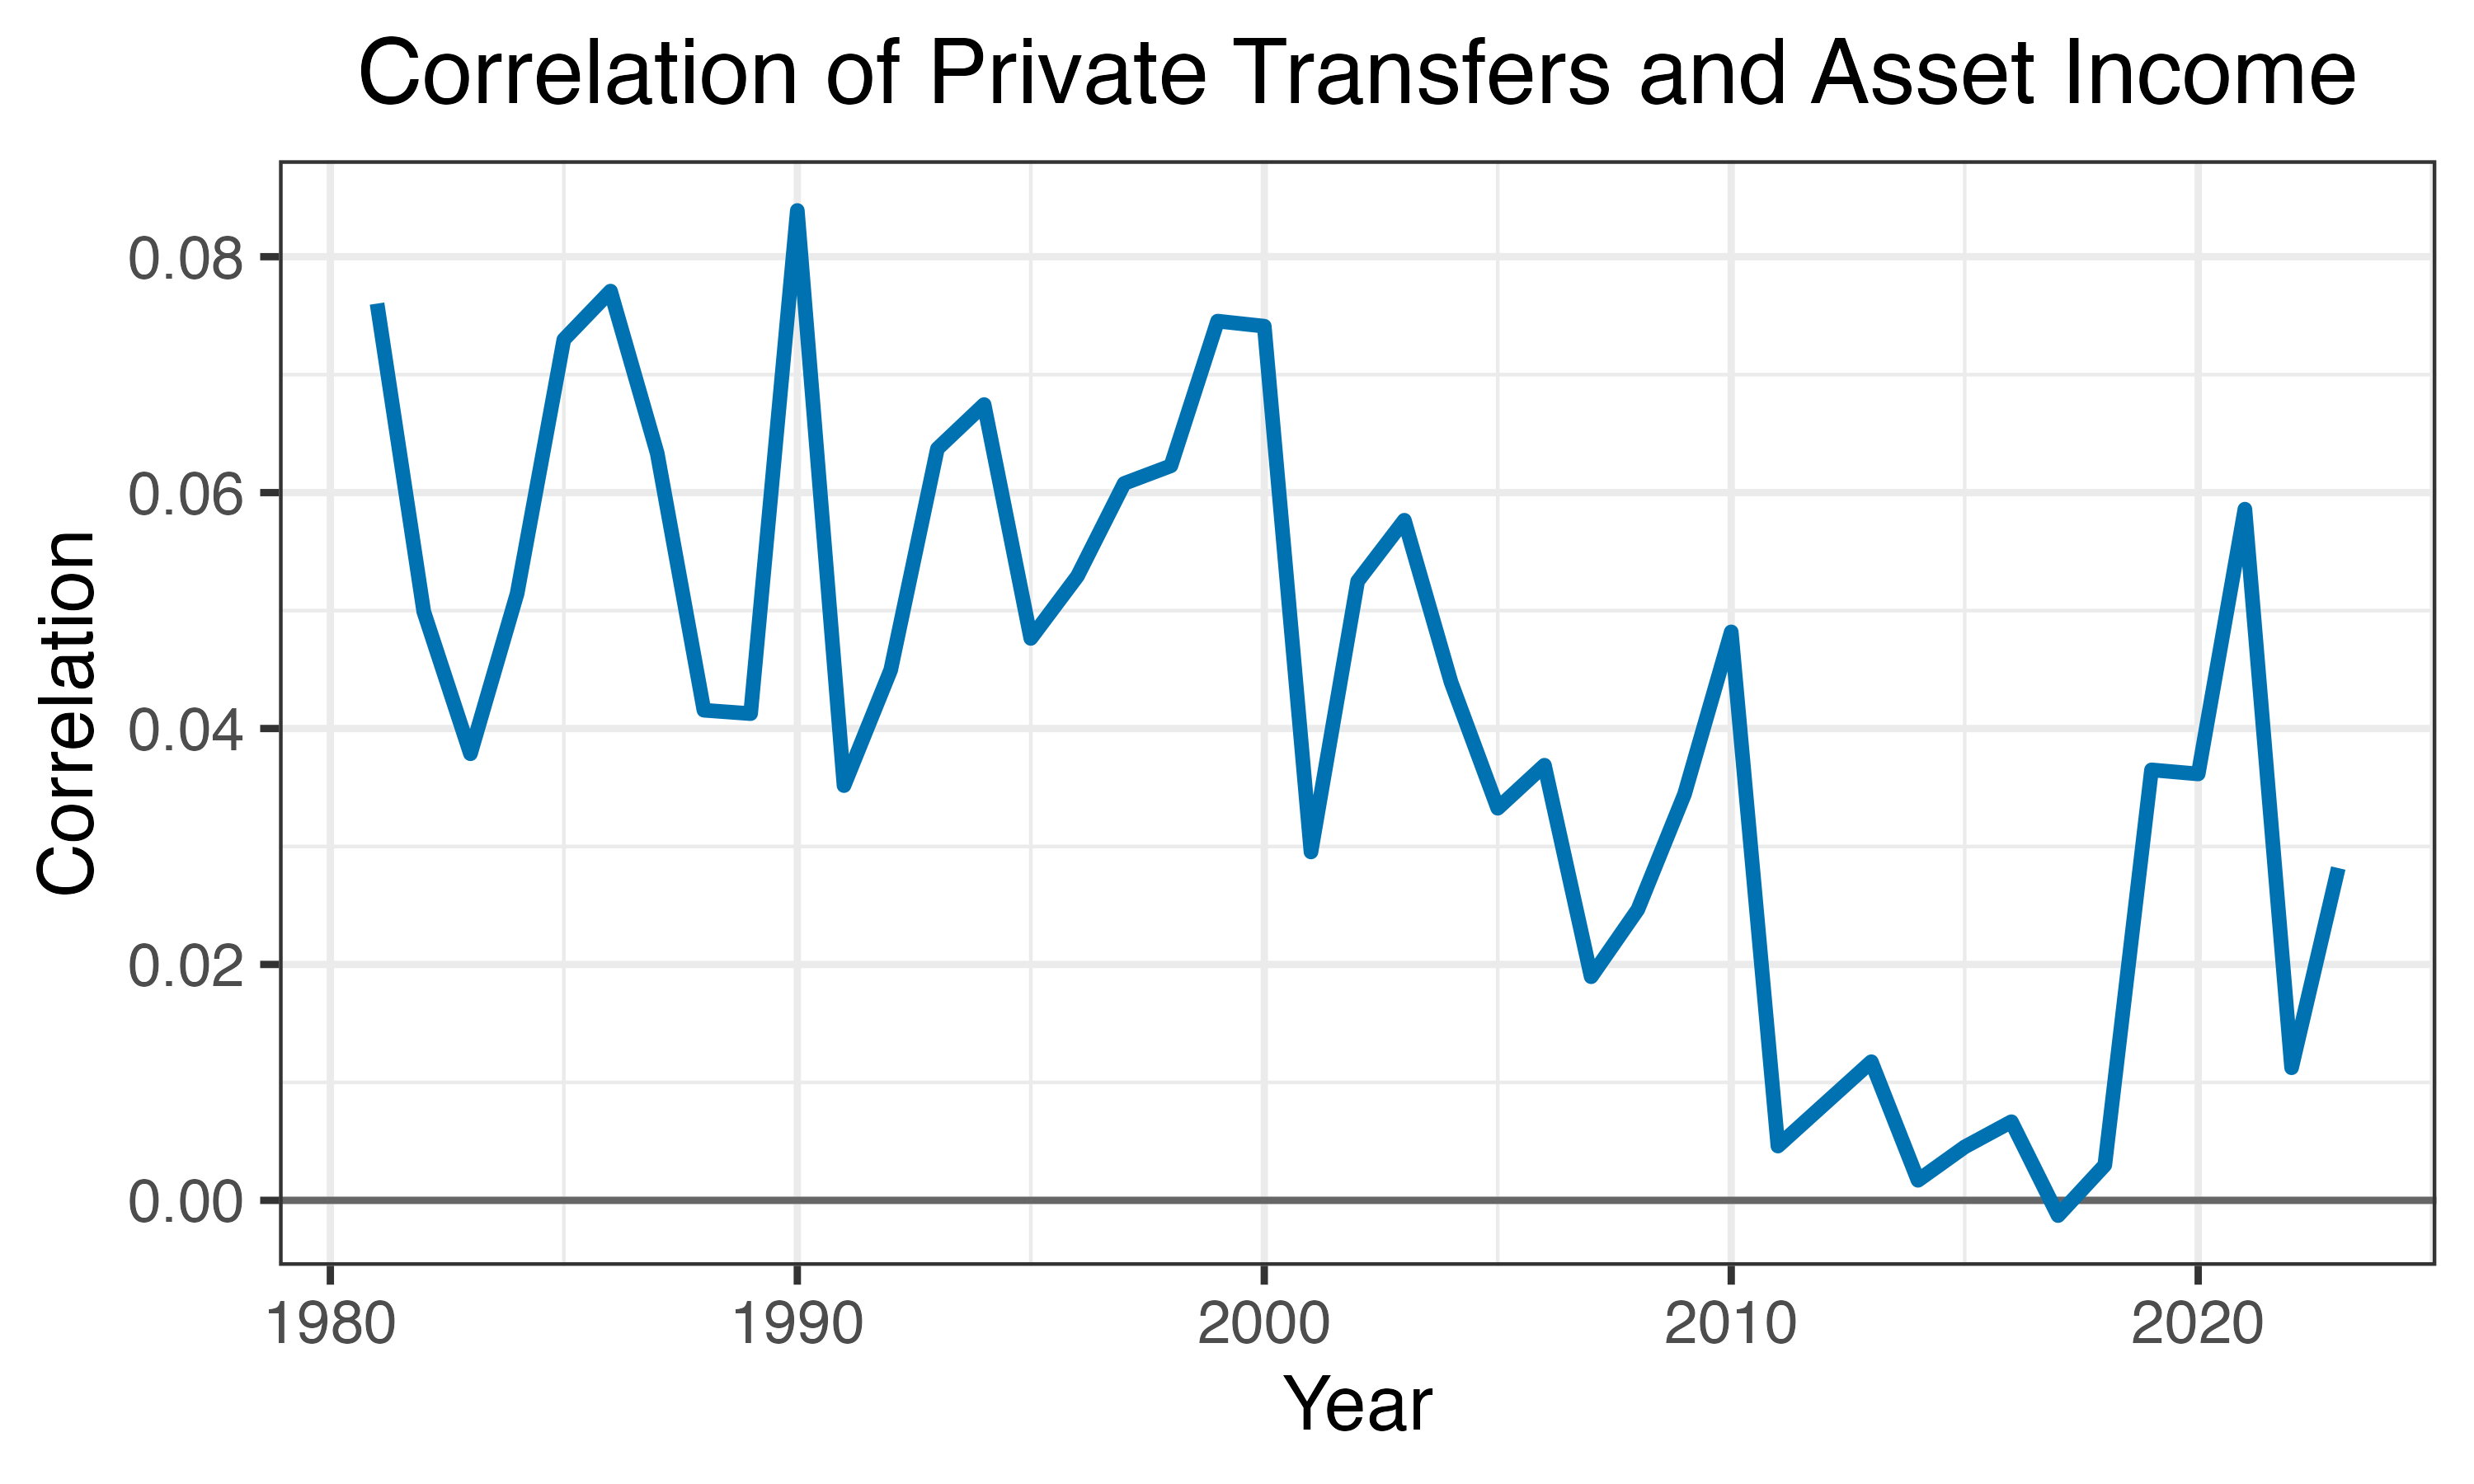
\includegraphics[width=0.6\textwidth]{figures/Fig_4/Fig_4e_corr_transfer_asset.png}
    \caption{Correlation of Private Transfers and Asset Income, 1981 - 2023}
    \label{fig:appendix_corr}
\end{figure}

\end{appendices}

\end{document}